% !TeX root = ../Book3.tex
% 纲要标题：# 第一编　度量、测地线与曲率结构
% 纲要位置：几何学计划纲要.md，第 2122 行。
% 正文状态：本编导读初稿；尚未正式审核。

% 纲要内容开始
% 
% 纲要内容结束

\BookPart{度量、测地线与曲率结构}{g3:part:01}
\BookPartGuide
球面的曲率处处相同，平坦环面的局部度量也很简单，两者却有不同的测地线和整体拓扑。比较这些空间，需要先把度量产生的几何量逐一构造出来。本编由切空间中的内积开始，建立长度、联络、曲率与子流形的基本语言，再研究平行移动所保留的整体结构。

\ProseParagraphBreak
\chapref{g3:ch:01}从度量构造体积密度、梯度和散度，并证明无挠度量联络的存在与唯一性。标架与结构方程把坐标计算改写成适于换标架的形式。\chapref{g3:ch:02}研究该联络的测地线：指数映射给出局部坐标，Gauss 引理联系径向曲线与最短路，Hopf--Rinow 定理再把距离完备性、测地完备性和闭有界集的紧性联系起来。割迹与注入半径记录这种局部描述在何处停止有效。

\ProseParagraphBreak
\chapref{g3:ch:03}把联络的二阶信息组织成曲率张量，比较截面曲率、Ricci 曲率与标量曲率，并用法坐标展开恢复它们对度量和体积的影响。\chapref{g3:ch:04}将环境联络分成切向与法向部分，得到第二基本形式和 Gauss、Codazzi、Ricci 相容方程；子流形基本定理进一步回答，满足相容条件的数据何时能够实现为浸入。

\ProseParagraphBreak
\chapref{g3:ch:05}从平行移动出发研究完整群、平行张量与分布。局部乘积结构在单连通和完备条件下提升为 de Rham 分解，齐性与对称空间则提供可计算的整体模型。特殊完整群和限制根专题可在需要时选读；它们分别连接后面的自旋、Kähler 与对称空间问题。

\ProseParagraphBreak
本编需要第一卷的切丛、联络、常微分方程与子流形基础；覆盖、Lie 群和分布的积分在相应位置使用。适合同时保留几个模型：用 Euclid 空间核查零曲率公式，用球面与双曲空间核查符号，用乘积和环面区分局部结构与整体商。后续比较理论以本编的指数映射、曲率约定及完备性结论为基础。

% !TeX root = ../../Book3.tex
% 纲要标题：## 第1章　黎曼度量与 Levi-Civita 联络
% 纲要位置：几何学计划纲要.md，第 2124 行。
% 正文状态：初稿；尚未正式审核。

% 纲要内容开始
% 
% > 本章目标与证明范围：从长度和度量相容性导出唯一无挠联络。公式必须能在坐标标架、正交标架和具体度量中互相核验；不把法坐标提前到指数映射之前。
% 
% 纲要内容结束

\chapter{黎曼度量与 Levi-Civita 联络}
\label{g3:ch:01}
\BookChapterNumber{g3:ch:01}

\begin{chapterabstract}
	光滑结构允许求导，黎曼度量进一步规定切向量的长度和夹角。本章由局部正定矩阵构造整体度量，建立梯度、体积密度、散度及分部积分公式；再从度量相容和无挠两个要求导出 Koszul 公式，证明 Levi-Civita 联络的存在唯一性。坐标标架与正交标架给出同一联络的两种表达，第一结构方程把无挠条件写成微分形式等式。诱导度量、乘积、共形变换和翘曲积展示这些公式的计算方式，二维模型与常数缩放则确定本卷的曲率符号和尺度约定。
\end{chapterabstract}

\begin{learninggoals}
	\begin{itemize}
		\item 从局部度量矩阵计算长度、梯度、体积密度与散度，并说明换坐标时这些几何量为何保持不变。
		\item 从度量相容和无挠条件推导 Koszul 公式，逐项验证它定义联络所需的线性及乘积法则。
		\item 在坐标标架和正交标架之间转换联络系数，用第一结构方程核验计算。
		\item 计算诱导、共形和翘曲积度量的联络，比较常数缩放对长度、体积和曲率的影响。
	\end{itemize}
\end{learninggoals}

在平面中，同一条曲线可以用直角坐标表示，也可以用极坐标表示。若曲线写成 \((r(t),\theta(t))\)，其速度的长度平方是
\[
	\dot r(t)^2+r(t)^2\dot\theta(t)^2.
\]
角度变化相同，在较大的圆周上走过的弧长就较长。这里的系数 \(r^2\) 记录坐标方向的实际尺度；它并不表示平面本身发生了弯曲。推广到流形时，我们在每个切空间上指定内积，并要求其系数随位置光滑变化。这使长度的定义脱离某一次坐标选择，也使没有预先嵌入空间的流形能够讨论体积和梯度。

\begin{figure}[htbp]
	\centering
	% !TeX root = ../Book3.tex
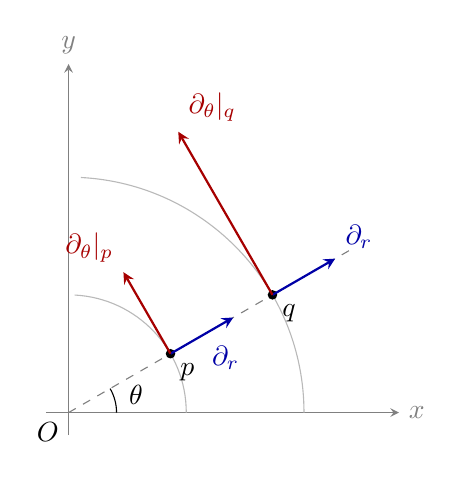
\begin{tikzpicture}[scale=1.15,>=stealth]
	\draw[->,gray] (-0.25,0)--(3.65,0) node[right]{\(x\)};
	\draw[->,gray] (0,-0.25)--(0,3.85) node[above]{\(y\)};
	\draw[gray!55] (0:1.3) arc[start angle=0,end angle=87,radius=1.3];
	\draw[gray!55] (0:2.6) arc[start angle=0,end angle=87,radius=2.6];
	\draw[dashed,gray] (0,0)--(30:3.6);
	\draw (0.53,0) arc[start angle=0,end angle=30,radius=0.53];
	\node at (15:0.77){\(\theta\)};
	\coordinate (P) at (30:1.3);
	\coordinate (Q) at (30:2.6);
	\fill (P) circle (1.5pt) node[below right]{\(p\)};
	\fill (Q) circle (1.5pt) node[below right]{\(q\)};
	\draw[->,thick,blue!65!black] (P)--++(30:0.8) node[midway,below right]{\(\partial_r\)};
	\draw[->,thick,blue!65!black] (Q)--++(30:0.8) node[above right]{\(\partial_r\)};
	\draw[->,thick,red!65!black] (P)--++(120:1.04) node[above left]{\(\partial_\theta|_p\)};
	\draw[->,thick,red!65!black] (Q)--++(120:2.08) node[above right]{\(\partial_\theta|_q\)};
	\node[below left] at (0,0){\(O\)};
\end{tikzpicture}

	\caption[极坐标方向的长度]{极坐标方向的长度。图中 \(q\) 的半径是 \(p\) 的两倍；用相同绘图比例表示向量时，两个径向坐标向量长度相同，角向坐标向量的长度则相差两倍。}
	\label{g3:fig:polar-coordinate-vectors}
\end{figure}

\cref{g3:fig:polar-coordinate-vectors}显示了度量如何记录坐标方向的尺度。有了长度，还需要比较邻近点的向量。在平面的极坐标标架中，径向和角向单位向量都随角度转动，所以只对向量的分量求导会漏掉标架本身的变化。联络把这部分变化计入导数。我们将要求这种导数满足内积的乘积法则，并使两个方向求导的反对称部分与向量场的括号一致。两个要求共同确定一个联络，其坐标表达和标架表达可以互相检验。

\ProseParagraphBreak

本章使用第一卷第11章的坐标图与切空间、第12章的张量和光滑单位分解，以及第14章的微分形式、密度积分和 Stokes 公式；每次实际调用时会恢复所需条件。\footnote{George Gabriel Stokes（1819--1903），生于爱尔兰的英国数学家、物理学家，研究流体力学与光学。}第一卷第15章学过的一般联络可帮助理解这些构造，本章仍给出切丛联络的定义和度量决定联络的证明。阅读本章无需先学第二卷的同调与同伦理论。度量给出曲线长度，长度的下确界如何成为距离、测地线如何产生法坐标，将在\chapref{g3:ch:02}展开。

\ProseParagraphBreak

以下光滑指 \(C^\infty\)，流形取有限维、Hausdorff、第二可数；除讨论边界积分时另作说明外，取实维数 \(n\ge1\) 且无边界。度量不要求可定向、紧或完备。坐标写为 \(x^1,\ldots,x^n\)，\(\partial_i\) 表示坐标向量场；同一单项式中重复的一个上指标和一个下指标表示从 \(1\) 到 \(n\) 求和。需要对照其他表述时，可参看 Petersen 第3版第1.1--1.2节和第1.4.2--1.4.4节的度量与标架、第2.2节和第2.4节的联络，以及第4.2.1节、第4.2.3节和第4.3.1节的球面与翘曲积模型\cite[第1.1--1.2节; 第1.4.2--1.4.4节; 第2.2节; 第2.4节; 第4.2.1节; 第4.2.3节; 第4.3.1节]{Petersen2016}。

% !TeX root = ../../Book3.tex
% 纲要标题：### 1.1 度量与几何量
% 纲要位置：几何学计划纲要.md，第 2128 行。
% 正文状态：初稿；尚未正式审核。

% 纲要内容开始
% 
% * 度量的存在及局部矩阵
% * 音乐同构、梯度和对偶度量
% * 体积密度、散度及分部积分
% * 坐标变化下的自然性
% 
% 纲要内容结束

\section{度量与几何量}
\label{g3:sec:0101}

一张坐标图能把曲线写成若干实函数，却没有规定哪个方向长、哪个方向短。即使在同一个平面上，\(\mathrm{d}x^2+\mathrm{d}y^2\) 与 \(4\,\mathrm{d}x^2+\mathrm{d}y^2\) 也给同一水平线段不同的长度。度量把这种测量规则放在每个切空间中，并要求它随点光滑变化。本节先说明度量怎样产生长度、梯度和体积，再由体积的变化定义散度；这些构造只需切丛、微分和积分，尚不需要比较不同点的向量。

\subsection{度量的存在及局部矩阵}
\label{g3:subsec:0101:01}

\begin{definition}
	\label{g3:def:riemannian-metric}
	设 \(M\) 是有限维、Hausdorff、第二可数的光滑流形。若光滑对称二阶协变张量场 \(g\) 在每个 \(p\in M\) 上给出正定双线性型 \(g_p\)，则称 \(g\) 为 \(M\) 上的\term[limanduliang]{黎曼度量}[Riemannian metric]，称 \((M,g)\) 为\term[limanliuxing]{黎曼流形}[Riemannian manifold]。向量的长度与非零向量之间的角度由
	\[
		|v|_g=\sqrt{g_p(v,v)},\qquad
		\cos\angle_g(v,w)=\frac{g_p(v,w)}{|v|_g|w|_g}
	\]
	确定。
\end{definition}
\symidx{\(g,g_{ij}\)：黎曼度量及其坐标分量}

这个名称纪念 Riemann。\footnote{Riemann，德文全名 Georg Friedrich Bernhard Riemann（1826--1866），德国数学家，在复分析、几何及分析学中作出基础性贡献。}本章讨论 \(n\geq1\) 维光滑流形，通常无边界；涉及边界时另行说明。取局部坐标 \((x^1,\ldots,x^n)\)，写 \(\partial_i=\partial/\partial x^i\)。度量具有表达
\begin{equation}
	\label{g3:eq:metric-local-matrix}
	g=g_{ij}\,\mathrm{d}x^i\otimes\mathrm{d}x^j,\qquad
	g_{ij}=g(\partial_i,\partial_j).
\end{equation}
这里及后文对重复的一上一下指标求和；完整求和有时仍写出以便辨认。矩阵 \(G=(g_{ij})\) 对称正定，各分量光滑。反之，一组这样的局部矩阵，只要在交叠处遵守张量变换规律，就确定一个度量。\(\mathrm{d}x^i\mathrm{d}x^j\) 等常见的线元简写在本章均按相应对称双线性型理解；特别地，\(2g_{12}\,\mathrm{d}x^1\mathrm{d}x^2\) 包含两个对称交叉项。

\begin{proposition}
	\label{g3:prop:metric-existence}
	每个有限维、Hausdorff、第二可数的光滑流形都存在黎曼度量，允许流形有边界。若 \(g_0,g_1\) 是两个这样的度量，则 \((1-t)g_0+tg_1\) 在 \(0\leq t\leq1\) 时仍是黎曼度量。
\end{proposition}
\begin{proof}
	第一卷第12.3节的光滑单位分解定理（定理 12.3.5）说明：对任意坐标覆盖 \(\{U_\alpha\}\)，可取非负光滑函数 \(\rho_\alpha\)，使支集族局部有限、\(\operatorname{supp}\rho_\alpha\subset U_\alpha\)，且 \(\sum_\alpha\rho_\alpha=1\)。在 \(U_\alpha\) 上把坐标标架规定为正交单位标架，得到局部度量 \(h_\alpha\)。令
	\[
		g=\sum_\alpha\rho_\alpha h_\alpha,
	\]
	其中每项在 \(U_\alpha\) 外补零。支集包含关系使补零光滑，局部有限性使和在每点附近只有有限项。对非零 \(v\in\mathrm{T}_pM\)，各非零权重对应的 \(h_\alpha(v,v)\) 都为正，又至少有一个权重为正，故 \(g_p(v,v)>0\)。这正是第一卷丛度量构造在切丛上的应用。最后，两个正数的非负凸组合仍正，直接给出度量族的正定性。
\end{proof}

存在性依靠正定型的凸性，并没有给流形指定一个首选度量。度量一旦选定，曲线的长度便有确定含义。

\begin{definition}
	\label{g3:def:riemannian-length}
	设 \((M,g)\) 为黎曼流形，\(\gamma:[a,b]\to M\) 是分片 \(C^1\) 曲线。其\term[quxianchangdu]{长度}[length]定义为
	\[
		L_g(\gamma)=\int_a^b|\dot\gamma(t)|_g\,\mathrm{d}t
		=\int_a^b\sqrt{g_{ij}(\gamma(t))\dot x^i(t)\dot x^j(t)}\,\mathrm{d}t,
	\]
	右侧坐标表达在曲线的各个坐标片上分别计算并相加。
\end{definition}

被积量是切向量的内在长度，因而换坐标不改变结果。若 \(t=\phi(s)\) 是区间之间的 \(C^1\) 微分同胚，则链式法则给出 \(|(\gamma\circ\phi)'(s)|_g=|\phi'(s)|\,|\dot\gamma(\phi(s))|_g\)，换元后得到长度不变；递增与递减参数均可。正定性保证非零速度的长度为正。用所有连接两点的曲线长度取下确界会得到内在距离，其正定性与距离拓扑将在\chapref{g3:ch:02}证明。

\begin{proposition}
	\label{g3:prop:metric-coordinate-bounds}
	设 \((M^n,g)\) 为光滑黎曼流形，\((U,x^1,\ldots,x^n)\) 是坐标图，\(K\subset U\) 是非空紧集。存在常数 \(0<c\leq C<\infty\)，使对 \(p\in K\) 和 \(v=v^i\partial_i\in\mathrm{T}_pM\)，有
	\[
		c\sum_i(v^i)^2\leq g_p(v,v)\leq C\sum_i(v^i)^2.
	\]
\end{proposition}
\begin{proof}
	函数 \((p,a)\mapsto g_{ij}(p)a^ia^j\) 在紧集 \(K\times S^{n-1}\) 上连续且处处为正，故取得正的最小值 \(c\) 和有限最大值 \(C\)。对非零坐标向量先除以其 Euclid 长度，再利用二次齐次性；零向量时两式均成立。\footnote{Euclid（\OriginalName{Εὐκλείδης}，拉丁转写 Eukleidēs，约公元前300年活动，确切生卒年不详），古希腊数学家，活动于 Alexandria，以《几何原本》对几何与数论的系统论述著称。}
\end{proof}

这个估计把几何长度与坐标长度联系起来：曲线留在 \(K\) 时，两种长度分别相差至多因子 \(\sqrt c\) 与 \(\sqrt C\)。紧性使常数能够统一选择；在整个非紧坐标域上，未必存在同一对常数。例如 \(\mathbb R\) 上的 \(g=e^{2x}\mathrm{d}x^2\) 处处正定，但相对于 \(\mathrm{d}x^2\) 既没有全局正下界，也没有全局有限上界。

\subsection{音乐同构、梯度和对偶度量}
\label{g3:subsec:0101:02}

微分 \(\mathrm{d}f_p\) 接受方向并返回函数的变化率，是协变向量；描述“增长最快的方向”却需要一个向量。度量通过内积配对把这两类对象联系起来。

\begin{definition}
	\label{g3:def:musical-isomorphisms}
	黎曼流形 \((M,g)\) 的\term[yinyuetonggou]{音乐同构}[musical isomorphisms]是互逆的光滑丛同构
	\[
		\flat_g:\mathrm{T}M\longrightarrow\mathrm{T}^*M,
		\quad v^{\flat_g}=g(v,\mathord\cdot),
		\qquad
		\sharp_g:\mathrm{T}^*M\longrightarrow\mathrm{T}M.
	\]
	\(\sharp_g\) 由 \(g(\alpha^{\sharp_g},v)=\alpha(v)\) 刻画。度量明确时省略符号中的下标 \(g\)。
\end{definition}

正定性使 \(v\mapsto g(v,\mathord\cdot)\) 单射，有限维且两边维数相同，所以它可逆。记 \((g^{ij})=G^{-1}\)，则
\begin{equation}
	\label{g3:eq:musical-coordinates}
	(v^\flat)_i=g_{ij}v^j,\qquad
	(\alpha^\sharp)^i=g^{ij}\alpha_j.
\end{equation}
逆矩阵可由余子式除以 \(\det G>0\) 表示，所以逆映射也光滑。名称中的两个符号分别来自降号与升号，恰好对应把分量的指标降低和升高；它们依赖 \(g\)，并非切空间与余切空间原有的识别。

\begin{definition}
	\label{g3:def:dual-metric-gradient}
	黎曼流形 \((M,g)\) 的\term[duiouduliang]{对偶度量}[dual metric]是余切丛上的内积
	\[
		g^{-1}(\alpha,\beta)=g(\alpha^\sharp,\beta^\sharp)
		=g^{ij}\alpha_i\beta_j.
	\]
	对光滑实函数 \(f\)，其\term[tidu]{梯度}[gradient]为 \(\operatorname{grad}_g f=(\mathrm{d}f)^\sharp\)，即满足
	\begin{equation}
		\label{g3:eq:gradient-definition}
		g(\operatorname{grad}_g f,X)=Xf,\qquad
		\operatorname{grad}_g f=g^{ij}(\partial_jf)\partial_i
	\end{equation}
	的唯一光滑向量场。
\end{definition}

\symidx{\(\flat_g,\sharp_g\)：由黎曼度量诱导的降指标与升指标同构}
\symidx{\(\operatorname{grad}_g f\)：函数相对于度量 \(g\) 的梯度}

在 \(\mathrm{d}f_p\ne0\) 处，对所有单位向量 \(v\) 有
\[
	\mathrm{d}f_p(v)=g_p(\operatorname{grad}_g f,v)
	\leq|\operatorname{grad}_g f|_g,
\]
等号恰在 \(v=\operatorname{grad}_g f/|\operatorname{grad}_g f|_g\) 时成立。这来自内积不等式及其等号条件，也说明“最快”是以 \(g\) 的单位长度为尺度。若 \(M\) 无边界，且 \(\mathrm{d}f\) 在非空水平集 \(S=f^{-1}(c)\) 上处处非零，则第一卷第11.4节的正则水平集定理（定理 11.4.4）给出 \(\mathrm{T}_pS=\ker\mathrm{d}f_p\)，故梯度与水平集正交；在临界点，梯度为零，不再给出一个单位法向。

\begin{example}
	\label{g3:exm:gradient-metric-dependence}
	在 \(\mathbb R^2\) 上取 \(g=4\,\mathrm{d}x^2+\mathrm{d}y^2\) 与 \(f=x+y\)。则
	\[
		\mathrm{d}f=\mathrm{d}x+\mathrm{d}y,\qquad
		\operatorname{grad}_g f=\tfrac14\partial_x+\partial_y,
		\qquad |\mathrm{d}f|_{g^{-1}}^2=\tfrac54.
	\]
	水平线 \(x+y=c\) 的切向量 \(\partial_x-\partial_y\) 与这个梯度的 \(g\) 配对为 \(4\cdot\tfrac14-1=0\)。若换成 Euclid 度量，梯度变为 \(\partial_x+\partial_y\)，而 \(\mathrm{d}f\) 本身不变。逆矩阵出现在梯度公式中，正是为了补偿各方向长度尺度的不同。
\end{example}

同一个度量还在各阶张量丛上给出内积。例如对二阶协变张量 \(A\)，有 \(|A|_g^2=g^{ik}g^{j\ell}A_{ij}A_{k\ell}\)；对微分 \(k\) 形式，若写成 \(\alpha=\frac1{k!}\alpha_{i_1\cdots i_k}\mathrm{d}x^{i_1}\wedge\cdots\wedge\mathrm{d}x^{i_k}\)，则
\[
	|\alpha|_g^2=\frac1{k!}
	g^{i_1j_1}\cdots g^{i_kj_k}
	\alpha_{i_1\cdots i_k}\alpha_{j_1\cdots j_k}.
\]
因子 \(1/k!\) 消去同一有序指标组的排列重复，使正交余标架中递增指标的楔积成为正交单位基。

\subsection{体积密度、散度及分部积分}
\label{g3:subsec:0101:03}

切空间中的内积还确定平行多面体的体积。对切向量组 \((v_1,\ldots,v_n)\)，其体积为内积矩阵 \((g(v_i,v_j))\) 行列式的非负平方根。换基矩阵若为 \(A\)，内积矩阵变为 \(A^{\mathsf T}GA\)，体积就乘以 \(|\det A|\)。这提示应使用绝对行列式变换的密度，而不必先选择定向。

\begin{definition}
	\label{g3:def:metric-volume-density}
	\(n\) 维黎曼流形 \((M,g)\) 的\term[tijimidu]{体积密度}[volume density]记为 \(\mu_g\)。在局部坐标 \((x^1,\ldots,x^n)\) 中令 \(G=(g_{ij})\) 为度量矩阵，则
	\begin{equation}
		\label{g3:eq:volume-density}
		\mu_g=\sqrt{\det G}\,|\mathrm{d}x^1\cdots\mathrm{d}x^n|.
	\end{equation}
	若另外给定定向，则在正向坐标中
	\[
		\operatorname{vol}_g=\sqrt{\det G}\,\mathrm{d}x^1\wedge\cdots\wedge\mathrm{d}x^n
	\]
	定义相应的\term[tijixingshi]{体积形式}[volume form]。
\end{definition}

\symidx{\(\mu_g\)：黎曼体积密度及相应测度}

密度符号中的竖线表示换坐标时取绝对行列式，不是对微分符号求绝对值。第一卷第14.3节的积分良定义定理（定理 14.3.4）已证明：将紧支光滑密度用单位分解拆到坐标片后，按通常多元积分求和，结果与坐标和分解无关。因此 \(\int_M f\mu_g\) 对紧支光滑 \(f\) 有定义，不要求 \(M\) 可定向。一般非负可测函数的体积积分可由这一光滑正密度所给的局部测度定义；本章的分部积分只用紧支光滑情形。定向反转会改变 \(\operatorname{vol}_g\) 的符号，却不改变 \(\mu_g\)。

\ProseParagraphBreak

散度测量向量场的流对体积的一阶改变。设 \(X\) 是无边界流形上的光滑向量场。第一卷第13.1节的最大局部流定理（定理 13.1.7）给出随 \((t,p)\) 光滑变化的局部微分同胚 \(\Phi_t\)，满足 \(\Phi_0=\operatorname{id}\) 与 \(\partial_t\Phi_t=X\circ\Phi_t\)。密度的\term[liedaoshu]{Lie 导数}[Lie derivative]定义为 \(\mathcal L_X\mu_g=\left.\frac{\mathrm{d}}{\mathrm{d}t}\right|_{t=0}\Phi_t^*\mu_g\)。\footnote{Lie，Marius Sophus Lie（1842--1899），挪威数学家，创立连续变换群理论，并研究其与微分方程的联系。}这里只需在每一点附近对足够小的 \(t\) 定义流，无需假设流对所有时间存在。由于 \(\mu_g\) 处处正，存在唯一光滑函数满足
\begin{equation}
	\label{g3:eq:divergence-definition}
	\mathcal L_X\mu_g=(\operatorname{div}_gX)\mu_g.
\end{equation}
这个函数称为 \(X\) 的\term[sandu]{散度}[divergence]。

\begin{proposition}
	\label{g3:prop:divergence-coordinate}
	在无边界黎曼流形 \((M,g)\) 的任一坐标图中，记 \(G=(g_{ij})\) 为度量矩阵。对光滑向量场 \(X=X^i\partial_i\)，有
	\begin{equation}
		\label{g3:eq:divergence-coordinate}
		\operatorname{div}_gX
		=\frac1{\sqrt{\det G}}\partial_i\bigl(\sqrt{\det G}\,X^i\bigr).
	\end{equation}
	因此，对光滑实函数 \(f\)，有
	\begin{equation}
		\label{g3:eq:divergence-product}
		\operatorname{div}_g(fX)=\mathrm{d}f(X)+f\operatorname{div}_gX.
	\end{equation}
	公式也唯一地延伸到带边界流形上光滑至边界的向量场。
\end{proposition}
\begin{proof}
	记 \(m=\sqrt{\det G}\)。局部流拉回密度的系数为 \(m(\Phi_t(x))|\det\mathrm{D}\Phi_t(x)|\)。在 \(t=0\) 时，\(\Phi_0=\operatorname{id}\)，且 \(\left.\partial_t\Phi_t\right|_0=X\)。行列式在单位矩阵处的一阶项是迹，故
	\[
		\left.\frac{\mathrm{d}}{\mathrm{d}t}\right|_0
		\bigl(m(\Phi_t(x))|\det\mathrm{D}\Phi_t(x)|\bigr)
		=X^i\partial_i m+m\partial_iX^i=\partial_i(mX^i).
	\]
	除以 \(m>0\) 即得坐标公式；对 \(fX\) 展开偏导数得到乘积公式。若流形有边界，坐标系数在半空间边界处仍光滑；不同边界图中的表达在稠密的内部相同，连续性使它们在边界也相同。这样定义边界处的散度，无须要求 \(X\) 的双侧流保留流形。
\end{proof}

在定向坐标片中，直接将 \(\iota_X\operatorname{vol}_g\) 写成缺少一个坐标微分的各项可得
\begin{equation}
	\label{g3:eq:divergence-exterior}
	\mathrm{d}(\iota_X\operatorname{vol}_g)
	=(\operatorname{div}_gX)\operatorname{vol}_g.
\end{equation}
这里 \(\iota_X\) 将 \(X\) 插入形式的第一个位置；各项的排列符号恰好使外微分的系数成为 \(\partial_i(mX^i)\)。由此可以把散度积分转成边界通量。

\ProseParagraphBreak

若 \(M\) 有光滑边界，限制 \(g\) 到 \(\mathrm{T}\partial M\) 就给出边界度量，记它的体积密度为 \(\mu_{\partial g}\)。在边界坐标中取定义函数 \(r\)，使 \(M\) 对应 \(r\geq0\)、边界对应 \(r=0\)，且边界上 \(\mathrm{d}r\ne0\)。于是 \(\nu=-\operatorname{grad}_g r/|\operatorname{grad}_g r|_g\) 是外单位法向。它由正交、单位长度和向外这三个条件唯一确定，所以不同边界图中的选择相容。

\begin{theorem}[散度定理]
	\label{g3:thm:divergence-theorem}
	设 \((M^n,g)\) 为有限维、Hausdorff、第二可数的光滑黎曼流形，\(n\geq1\)，允许有光滑边界，无须可定向。若 \(X\) 是光滑至边界的紧支向量场，\(\nu\) 是边界的外单位法向，\(\mu_{\partial g}\) 是边界诱导度量的体积密度，则
	\begin{equation}
		\label{g3:eq:divergence-theorem}
		\int_M\operatorname{div}_gX\,\mu_g
		=\int_{\partial M}g(X,\nu)\,\mu_{\partial g}.
	\end{equation}
	无边界时右侧为零；\(n=1\) 时边界积分按各端点的计数密度求和。
\end{theorem}
\begin{proof}
	先假设 \(X\) 的支集位于一张坐标片 \(U\) 内并紧含于该片。给 \(U\) 任选定向，对紧支形式 \(\iota_X\operatorname{vol}_g\) 使用第一卷第14.4节的 Stokes 定理（定理 14.4.3）：外微分的积分等于在外法向优先定向下的边界积分。由\eqref{g3:eq:divergence-exterior}，左边就是散度乘以正体积密度的积分。

	当 \(n\geq2\) 时，在边界点取正交单位基 \((\nu,e_1,\ldots,e_{n-1})\)，使它符合 \(U\) 的定向。把 \(X\) 分成法向部分 \(g(X,\nu)\nu\) 和切向部分，切向部分与其余 \(n-1\) 个切向量线性相关，因而在顶次形式中贡献为零。故
	\[
		(\iota_X\operatorname{vol}_g)(e_1,\ldots,e_{n-1})=g(X,\nu).
	\]
	所以边界项正是 \(g(X,\nu)\mu_{\partial g}\) 的积分。\(n=1\) 时，在正向单位切向量为 \(e\) 的记号下，若 \(\nu=\varepsilon e\)，边界点的诱导定向符号就是 \(\varepsilon\)；其贡献为 \(\varepsilon\operatorname{vol}_g(X)=g(X,\nu)\)，结论相同。反转所选定向会同时反转体积形式与边界定向，两个密度积分都不变，所得局部公式不依赖这次选择。

	一般情形取从属于坐标覆盖的光滑单位分解 \(\{\rho_\alpha\}\)。紧支性及局部有限性保证只有有限个 \(\rho_\alpha X\) 非零，且各项支集紧含于相应坐标片。逐项应用局部公式并相加。乘积公式给出
	\[
		\sum_\alpha\operatorname{div}_g(\rho_\alpha X)
		=\Bigl(\sum_\alpha\rho_\alpha\Bigr)\operatorname{div}_gX
		+X\Bigl(\sum_\alpha\rho_\alpha\Bigr)
		=\operatorname{div}_gX,
	\]
	边界通量的和也等于 \(g(X,\nu)\)。这证明全局公式，包括不可定向情形。
\end{proof}

把定理应用于 \(fX\)，得到分部积分的基本形式。若 \(f\) 光滑、\(X\) 光滑，且其中至少一个紧支，则
\begin{equation}
	\label{g3:eq:integration-by-parts}
	\int_M f\operatorname{div}_gX\,\mu_g
	=-\int_M g(\operatorname{grad}_g f,X)\,\mu_g
	+\int_{\partial M}f g(X,\nu)\,\mu_{\partial g}.
\end{equation}
在带边界情形，所有数据都要求光滑至边界。无边界、\(f\) 在边界为零，或 \(X\) 沿边界切向时，边界项消失。非紧流形上的支集条件则控制无穷远的通量，不能从公式中直接删除。

\begin{definition}
	\label{g3:def:laplace-beltrami}
	设 \((M,g)\) 为光滑黎曼流形，\(f\in C^\infty(M;\mathbb R)\)。在局部坐标中记 \(G=(g_{ij})\)、\((g^{ij})=G^{-1}\)。采用\term[laplacebeltramisuanzi]{Laplace--Beltrami 算子}[Laplace--Beltrami operator]的非负号约定
	\begin{equation}
		\label{g3:eq:laplace-beltrami}
		\Delta_g f\coloneqq-\operatorname{div}_g(\operatorname{grad}_g f)
		=-\frac1{\sqrt{\det G}}
		\partial_i\bigl(\sqrt{\det G}\,g^{ij}\partial_jf\bigr).
	\end{equation}
\end{definition}

\symidx{\(\operatorname{div}_g X\)：向量场相对于黎曼体积的散度}
\symidx{\(\Delta_g\)：函数上的非负 Laplace 算子 \(-\operatorname{div}_g\operatorname{grad}_g\)}

这个名称沿用 Laplace 和 Beltrami 的姓氏。\footnote{Laplace，法文全名 Pierre-Simon Laplace（1749--1827），法国数学家和天文学家，研究概率、势函数与天体力学。Beltrami，意大利文名 Eugenio Beltrami（1835--1900），意大利数学家，研究微分几何、非 Euclid 几何模型及微分算子。}具体说，无边界时，对 \(u,v\in C_c^\infty(M)\)，分部积分给出
\begin{equation}
	\label{g3:eq:laplace-energy}
	\int_M u\Delta_gv\,\mu_g
	=\int_M g(\operatorname{grad}_g u,\operatorname{grad}_g v)\,\mu_g
	=\int_M v\Delta_gu\,\mu_g.
\end{equation}
令 \(u=v\)，便有 \(\int_Mu\Delta_gu\,\mu_g\geq0\)。这说明本书的非负号约定指积分二次型非负，不是说每个非负函数的 \(\Delta_g\) 仍逐点非负。带边界时，对光滑至边界的紧支函数 \(u,v\)，相应公式为
\[
	\int_Mu\Delta_gv\,\mu_g
	=\int_M g(\operatorname{grad}_g u,\operatorname{grad}_g v)\,\mu_g
	-\int_{\partial M}u\partial_\nu v\,\mu_{\partial g},
\]
其中 \(\partial_\nu v=\mathrm{d}v(\nu)\)。例如两函数都在边界为零时，仍得到\eqref{g3:eq:laplace-energy}的对称关系。

\begin{example}
	\label{g3:exm:polar-metric-operators}
	在平面去掉原点后的一个角度坐标片上，Euclid 度量写为
	\[
		g=\mathrm{d}r^2+r^2\mathrm{d}\theta^2,\qquad
		\mu_g=r|\mathrm{d}r\,\mathrm{d}\theta|.
	\]
	对任意光滑实函数 \(f\) 及光滑向量场 \(X=X^r\partial_r+X^\theta\partial_\theta\)，有
	\[
		\begin{aligned}
			\operatorname{grad}_g f
			&=f_r\partial_r+r^{-2}f_\theta\partial_\theta,\\
			\operatorname{div}_g X
			&=r^{-1}\partial_r(rX^r)+\partial_\theta X^\theta,\\
			\Delta_g f
			&=-f_{rr}-r^{-1}f_r-r^{-2}f_{\theta\theta}.
		\end{aligned}
	\]
	这里 \(X^\theta\) 是相对于 \(\partial_\theta\) 的系数；若改用单位向量 \(r^{-1}\partial_\theta\) 的系数，散度的角向项也必须相应改写。例如 \(X=\partial_r\) 满足 \(\operatorname{div}_gX=1/r\)：向外移动厚度相同的小扇环，其周长随半径增长。原点不属于这张坐标图，公式中的 \(1/r\) 不表示原平面的度量在原点有奇性。
\end{example}

\subsection{坐标变化下的自然性}
\label{g3:subsec:0101:04}

前面的公式都含矩阵逆、行列式和偏导数。它们能否给出同一个几何对象，取决于这些变化是否彼此抵消。先直接核对换坐标，再把结论表述为局部等距下的相容性。

\ProseParagraphBreak

在交叠坐标 \(x=x(y)\) 中，记 \(J^i{}_a=\partial x^i/\partial y^a\)。由 \(\partial/\partial y^a=J^i{}_a\partial_i\)，新矩阵满足
\begin{equation}
	\label{g3:eq:metric-coordinate-transformation}
	G_y=J^{\mathsf T}G_xJ,\qquad
	G_y^{-1}=J^{-1}G_x^{-1}(J^{\mathsf T})^{-1},\qquad
	\sqrt{\det G_y}=|\det J|\sqrt{\det G_x}.
\end{equation}
第一式是双线性型的换基，第二式保证升指标后得到向量的变换规律，第三式恰是密度的变换规律。因此 \(g^{-1}\)、梯度和 \(\mu_g\) 的局部表达在交叠处相容；散度由局部流定义，也与坐标选择无关。

\begin{definition}
	\label{g3:def:local-isometry}
	设 \((M,g)\)、\((N,h)\) 是黎曼流形。若光滑映射 \(F:M\to N\) 是局部微分同胚且 \(F^*h=g\)，即
	\[
		h_{F(p)}(\mathrm{d}F_pv,\mathrm{d}F_pw)=g_p(v,w),
	\]
	则称 \(F\) 为\term[jubudengju]{局部等距}[local isometry]。若它还是微分同胚，则称为\term[dengju]{等距}[isometry]。
\end{definition}

\begin{proposition}
	\label{g3:prop:metric-naturality}
	设 \(F:(M,g)\to(N,h)\) 是无边界黎曼流形间的局部等距，\(f\in C^\infty(N)\)。则
	\[
		F^*\mu_h=\mu_g,\qquad
		\mathrm{d}F\bigl(\operatorname{grad}_g(f\circ F)\bigr)
		=(\operatorname{grad}_h f)\circ F,
	\]
	且对任意分片 \(C^1\) 曲线 \(\gamma\)，有 \(L_h(F\circ\gamma)=L_g(\gamma)\)。若 \(M\)、\(N\) 上的光滑向量场分别为 \(X\)、\(Y\)，且满足 \(\mathrm{d}F(X)=Y\circ F\)，则
	\[
		\operatorname{div}_gX=(\operatorname{div}_hY)\circ F,
		\qquad \Delta_g(f\circ F)=(\Delta_h f)\circ F.
	\]
\end{proposition}
\begin{proof}
	密度等式由\eqref{g3:eq:metric-coordinate-transformation}的行列式关系得出，长度等式由 \(\mathrm{d}F\) 逐点保持速度的内积得出。对任意 \(v\in\mathrm{T}_pM\)，有
	\[
		\begin{aligned}
			h\bigl(\mathrm{d}F\operatorname{grad}_g(f\circ F),\mathrm{d}Fv\bigr)
			&=\mathrm{d}(f\circ F)(v)\\
			&=\mathrm{d}f(\mathrm{d}Fv)
			=h\bigl(\operatorname{grad}_h f,\mathrm{d}Fv\bigr).
		\end{aligned}
	\]
	因 \(\mathrm{d}F_p\) 满射且 \(h\) 非退化，得到梯度关系。

	最后把 \(F\) 限制在可逆的邻域中，在目标选择坐标 \(y\)，源上取 \(x=y\circ F\)。相关向量场在这两套对应坐标中的分量相同，\(G(x)=H(y)\) 也对应相同。因此\eqref{g3:eq:divergence-coordinate}在对应点给出同一实数，证明散度关系。将它用于刚得到的梯度关系，再带入 \(\Delta=-\operatorname{div}\operatorname{grad}\)，便得到最后一个等式。
\end{proof}

局部等距可以重复覆盖同一个区域。例如 \(\mathbb R\to S^1\)、\(t\mapsto(\cos t,\sin t)\)，对 \(\mathrm{d}t^2\) 与单位圆的诱导度量是局部等距，它保持每条参数曲线的长度，却不保持整个空间的总体积。积分换元还需整体条件：若 \(F\) 是等距、\(f\in C_c^\infty(N)\)，则第一卷定理 14.3.6 的密度换元给出 \(\int_M(f\circ F)\mu_g=\int_Nf\mu_h\)；若仅有局部等距，重叠覆盖的次数可能改变积分。矩阵变换、局部几何量和整体积分因而各自有清楚的适用范围。

% !TeX root = ../../Book3.tex
% 纲要标题：### 1.2 Levi-Civita 定理
% 纲要位置：几何学计划纲要.md，第 2135 行。
% 正文状态：初稿；尚未正式审核。

% 纲要内容开始
% 
% * 度量相容与无挠性
% * Koszul 公式的推导
% * Levi-Civita 联络的构造
% * 存在唯一性及 Christoffel 表达
% 
% 纲要内容结束

\section{Levi-Civita 定理}
\label{g3:sec:0102}

度量使同一切空间中的向量可以比较长度和夹角。要对向量场求导，还须比较不同点的切空间。坐标分量的普通导数会随坐标改变，因为坐标基向量本身也在变化；联络给导数补上这部分变化。现在的问题是：给定度量以后，能否选出一种与长度相容、又保留普通微分交换规则的联络？

\subsection{度量相容与无挠性}
\label{g3:subsec:0102:01}

先恢复第一卷第15.1节的联络定义。在光滑流形 \(M\) 上，一个切丛联络是实双线性运算 \((X,Y)\mapsto\nabla_XY\)，并满足
\begin{equation}\label{g3:eq:connection-rules}
	\nabla_{fX}Y=f\nabla_XY,\qquad
	\nabla_X(fY)=X(f)Y+f\nabla_XY,
	\qquad f\in C^\infty(M).
\end{equation}
第一个输入是求导方向，所以只依赖该方向在当前点的值；第二个输入是待微分的向量场，所以必须保留其分量的导数。第一卷命题15.1.2“联络的局部性”说明，对有限维、Hausdorff、第二可数光滑流形上的有限秩光滑丛，联络可唯一限制到任意开集，且在方向输入上只依赖点值。切丛满足这些条件；下文使用局部向量场时均取这种限制。
% 跨卷依赖：g1:def:bundle-connection，g1:prop:connection-locality。

\begin{definition}\label{g3:def:metric-torsion-conditions}
	设 \((M,g)\) 为光滑黎曼流形，\(\nabla\) 为其切丛联络。若对任意光滑向量场 \(X,Y,Z\)，有
	\begin{equation}\label{g3:eq:metric-compatibility}
		X\bigl(g(Y,Z)\bigr)=g(\nabla_XY,Z)+g(Y,\nabla_XZ),
	\end{equation}
	则称 \(\nabla\) 与 \(g\) \term[duliangxiangrong]{度量相容}[metric compatible]。联络的\term[naolv]{挠率}[torsion]是
	\begin{equation}\label{g3:eq:torsion-definition}
		T^\nabla(X,Y)=\nabla_XY-\nabla_YX-[X,Y].
	\end{equation}
	若 \(T^\nabla=0\)，则称 \(\nabla\) \term[wunao]{无挠}[torsion free]。
\end{definition}

相容条件把内积的求导写成乘积规则。第一卷命题15.2.9“度量相容与平行移动”说明，对带光滑正定丛度量的有限秩实向量丛，这等价于沿每条有限分片光滑路径的平行移动保持内积。应用于切丛时，沿光滑曲线的平行向量场满足 \(\mathrm{D}_tV=\mathrm{D}_tW=0\)，于是 \(\frac{\mathrm{d}}{\mathrm{d}t}g(V,W)=g(\mathrm{D}_tV,W)+g(V,\mathrm{D}_tW)=0\)。无挠条件则比较交换两个向量场后的导数：Euclid 空间的普通导数满足 \(\mathrm{D}_XY-\mathrm{D}_YX=[X,Y]\)，式\eqref{g3:eq:torsion-definition}度量的正是对这条恒等式的偏离。这里的挠率是向量值二形式，与空间曲线的标量挠率不同。
% 跨卷依赖：g1:prop:metric-parallel-transport。

\begin{proposition}\label{g3:prop:connection-difference-conditions}
	设 \((M,g)\) 为光滑黎曼流形，\(\nabla,\widehat\nabla\) 为光滑切丛联络，令
	\[
		A(X,Y)=\widehat\nabla_XY-\nabla_XY.
	\]
	则 \(A\) 对两个输入都为 \(C^\infty(M)\) 线性，挠率 \(T^\nabla\) 也对两个输入都为 \(C^\infty(M)\) 线性。若 \(\nabla\) 已与 \(g\) 相容，则 \(\widehat\nabla\) 与 \(g\) 相容当且仅当
	\[
		g(A(X,Y),Z)+g(Y,A(X,Z))=0.
	\]
	若 \(\nabla\) 无挠，则 \(\widehat\nabla\) 无挠当且仅当 \(A(X,Y)=A(Y,X)\)。
\end{proposition}
\begin{proof}
	两联络的乘积规则相减时，含 \(X(f)Y\) 的项相消，故 \(A(X,fY)=fA(X,Y)\)；第一个输入的函数线性直接由定义得到。对挠率，利用 \([fX,Y]=f[X,Y]-Y(f)X\)，有
	\[
		T^\nabla(fX,Y)
		=f\nabla_XY-Y(f)X-f\nabla_YX-f[X,Y]+Y(f)X
		=fT^\nabla(X,Y).
	\]
	第二个输入的函数线性再由反对称性得到。最后，将 \(\widehat\nabla=\nabla+A\) 代入相容条件和挠率定义，分别作差，即得后两项。
\end{proof}

\begin{example}\label{g3:exm:compatibility-torsion-independent}
	在 Euclid 平面上，记 \(g_0=\mathrm{d}x^2+\mathrm{d}y^2\)，\(\mathrm{D}\) 为通常导数，\(J\partial_x=\partial_y\)、\(J\partial_y=-\partial_x\)。定义
	\[
		\nabla^a_XY=\mathrm{D}_XY+\mathrm{d}x(X)JY.
	\]
	由于 \(J\) 关于 \(g_0\) 反对称，上一个命题说明 \(\nabla^a\) 与 \(g_0\) 相容；但
	\[
		T^{\nabla^a}(\partial_x,\partial_y)=J\partial_y=-\partial_x\ne0.
	\]
	再定义
	\[
		\nabla^b_XY=\mathrm{D}_XY+\mathrm{d}x(X)\mathrm{d}x(Y)\partial_x.
	\]
	新增项关于 \(X,Y\) 对称，故 \(\nabla^b\) 无挠。然而 \(\nabla^b_{\partial_x}\partial_x=\partial_x\)，所以
	\[
		\partial_xg_0(\partial_x,\partial_x)=0,
		\qquad
		2g_0(\nabla^b_{\partial_x}\partial_x,\partial_x)=2.
	\]
	它不与 \(g_0\) 相容。两项要求分别约束联络，必须同时使用才能选出本节所求的联络。
\end{example}

\subsection{Koszul 公式的推导}
\label{g3:subsec:0102:02}

假设相容且无挠的联络已经存在，先求出它必定满足的公式。对 \(X,Y,Z\) 循环使用度量相容性，得到
\begin{align*}
	Xg(Y,Z)&=g(\nabla_XY,Z)+g(Y,\nabla_XZ),\\
	Yg(Z,X)&=g(\nabla_YZ,X)+g(Z,\nabla_YX),\\
	Zg(X,Y)&=g(\nabla_ZX,Y)+g(X,\nabla_ZY).
\end{align*}
将前两式相加再减去第三式。无挠性给出
\[
	\nabla_YX=\nabla_XY-[X,Y],\qquad
	\nabla_XZ-\nabla_ZX=[X,Z],\qquad
	\nabla_YZ-\nabla_ZY=[Y,Z].
\]
代入后，所有未知导数合成 \(2g(\nabla_XY,Z)\)，得到\term[koszulgongshi]{Koszul 公式}[Koszul formula]：\footnote{Jean-Louis Koszul（1921--2018），法国数学家，研究 Lie 代数上同调、齐性空间和微分几何，其工作也产生了同调代数中的 Koszul 复形。}
\begin{equation}\label{g3:eq:koszul-formula}
	\begin{aligned}
		2g(\nabla_XY,Z)
		={}&Xg(Y,Z)+Yg(Z,X)-Zg(X,Y)\\
		&-g(X,[Y,Z])+g(Y,[Z,X])+g(Z,[X,Y]).
	\end{aligned}
\end{equation}
右侧只含给定的度量、向量场及其括号。固定 \(X,Y\) 后，若知道 \(g(\nabla_XY,Z)\) 对所有 \(Z\) 的值，正定内积便唯一确定 \(\nabla_XY\)。因此唯一性已经蕴含在此公式中；存在性还须确认右侧确实定义联络。

\subsection{Levi-Civita 联络的构造}
\label{g3:subsec:0102:03}

把式\eqref{g3:eq:koszul-formula}右侧的一半记为 \(B(X,Y,Z)\)。其中单项含有 \(Z\) 的导数，但这些导数必须相消，才能使 \(Z\mapsto B(X,Y,Z)\) 是一点处的线性泛函。这是从公式恢复向量的关键。

\begin{lemma}\label{g3:lem:koszul-construction}
	设 \((M,g)\) 为有限维、Hausdorff、第二可数、无边界的光滑黎曼流形，对任意光滑向量场 \(X,Y,Z\)，将式\eqref{g3:eq:koszul-formula}右侧的一半记为 \(B(X,Y,Z)\)。则对光滑实函数 \(f\in C^\infty(M)\) 有
	\begin{align*}
		B(fX,Y,Z)&=fB(X,Y,Z),\\
		B(X,fY,Z)&=fB(X,Y,Z)+X(f)g(Y,Z),\\
		B(X,Y,fZ)&=fB(X,Y,Z).
	\end{align*}
	由 \(g(\nabla_XY,Z)=B(X,Y,Z)\) 唯一确定的 \(\nabla\) 是光滑切丛联络，并且与 \(g\) 相容且无挠。
\end{lemma}
\begin{proof}
	三个等式均由乘积规则和括号的乘法公式得到。为说明导数如何消去，先把第三个输入换成 \(fZ\)。在 \(2B(X,Y,fZ)\) 中，除共同因子 \(f\) 外，多出的四项是
	\[
		X(f)g(Y,Z)+Y(f)g(Z,X)-Y(f)g(X,Z)-X(f)g(Y,Z)=0.
	\]
	换第一个输入为 \(fX\) 时，多出的四项是
	\[
		Y(f)g(Z,X)-Z(f)g(X,Y)+Z(f)g(Y,X)-Y(f)g(Z,X)=0.
	\]
	换第二个输入为 \(fY\) 时，多出
	\[
		X(f)g(Y,Z)-Z(f)g(X,Y)+Z(f)g(X,Y)+X(f)g(Z,Y)
		=2X(f)g(Y,Z).
	\]
	这证明了三条规则。

	在任一坐标区域写 \(Z=Z^i\partial_i\)。第三条规则说明
	\[
		B(X,Y,Z)=Z^iB(X,Y,\partial_i),
	\]
	所以它是光滑一形式对 \(Z\) 的求值。利用度量的音乐同构，定义
	\[
		\nabla_XY
		=g^{ij}B(X,Y,\partial_i)\partial_j.
	\]
	它光滑且满足规定的内积等式。不同坐标给出的向量与任意 \(Z\) 都有同一内积，因而相同，故各局部定义粘合为整体运算。第一、第二条规则以及正定性分别给出式\eqref{g3:eq:connection-rules}中的两个等式；实双线性直接来自 \(B\) 的表达式。

	还须验证原来要求的两个几何性质。把 \(B\) 的六项表达式分别交换第二、第三个输入后相加，可得
	\[
		B(X,Y,Z)+B(X,Z,Y)=Xg(Y,Z).
	\]
	其中括号项成对相消，度量导数只留下右侧。因此所得联络与度量相容。交换第一、第二个输入再相减，则得
	\[
		B(X,Y,Z)-B(Y,X,Z)=g([X,Y],Z).
	\]
	这说明 \(g(\nabla_XY-\nabla_YX-[X,Y],Z)=0\) 对所有 \(Z\) 成立，故挠率为零。
\end{proof}

这一构造无需先选一个背景联络再作修正。度量把右侧的一形式变成向量，而公式的函数线性保证局部定义彼此相容。它也说明，联络取决于度量的一阶变化，单独知道一个点上的内积还不足以算出附近向量场的协变导数。

\subsection{存在唯一性及 Christoffel 表达}
\label{g3:subsec:0102:04}

现在可以将上述推导与构造合为黎曼几何的基本存在唯一性定理。所得联络称为\term[levicivitalianluo]{Levi-Civita 联络}[Levi-Civita connection]。\footnote{Tullio Levi-Civita（1873--1941），意大利数学家，对绝对微分学、张量分析及微分几何作出重要贡献。}

\termidx[Levi Civita dingli]{Levi-Civita 定理}
\foreignidx{Levi-Civita theorem}
\begin{theorem}[Levi-Civita 定理]\label{g3:thm:levi-civita}
	设 \(M\) 为有限维、Hausdorff、第二可数、无边界的光滑流形，\(g\) 为其光滑黎曼度量。则 \(\mathrm{T}M\) 上存在唯一与 \(g\) 相容且无挠的光滑联络。它由 Koszul 公式\eqref{g3:eq:koszul-formula}确定。
\end{theorem}
\symidx{\(\nabla\)：黎曼度量的 Levi-Civita 联络}
\begin{proof}
	\cref{g3:lem:koszul-construction}给出存在性。任一相容且无挠的联络均满足式\eqref{g3:eq:koszul-formula}，而非退化内积唯一确定左侧的 \(\nabla_XY\)，所以联络唯一。
\end{proof}

在局部坐标 \((x^1,\ldots,x^n)\) 中，以
\[
	\nabla_{\partial_i}\partial_j=\Gamma^k_{ij}\partial_k
\]
定义\term[christoffelfuhao]{Christoffel 符号}[Christoffel symbols]。\footnote{Elwin Bruno Christoffel（1829--1900），德国数学家，研究微分形式的变换、不变量和复分析，其工作推动了协变微分与张量分析的发展。}由于坐标向量场两两交换，Koszul 公式简化为
\[
	2g_{k\ell}\Gamma^k_{ij}=\partial_i g_{j\ell}+\partial_jg_{i\ell}-\partial_\ell g_{ij}.
\]
用逆矩阵升起指标，得到
\begin{equation}\label{g3:eq:christoffel-metric}
	\Gamma^k_{ij}
	=\frac12g^{k\ell}
	\bigl(\partial_i g_{j\ell}+\partial_jg_{i\ell}-\partial_\ell g_{ij}\bigr).
\end{equation}
\symidx{\(\Gamma^k_{ij}\)：Levi-Civita 联络的坐标系数}
因此任意向量场的协变导数为
\begin{equation}\label{g3:eq:coordinate-covariant-derivative}
	\nabla_XY
	=\left(X^i\partial_iY^k+\Gamma^k_{ij}X^iY^j\right)\partial_k.
\end{equation}
下指标 \(i,j\) 的对称性表达无挠条件；相容性则等价于
\[
	\partial_i g_{jk}=\Gamma^\ell_{ij}g_{\ell k}+\Gamma^\ell_{ik}g_{j\ell}.
\]

\begin{example}\label{g3:exm:polar-christoffel}
	在 Euclid 平面的极坐标局部区域 \(r>0\) 中，\(g=\mathrm{d}r^2+r^2\mathrm{d}\varphi^2\)。度量矩阵为 \(\operatorname{diag}(1,r^2)\)，只有 \(\partial_rg_{\varphi\varphi}=2r\) 非零。由式\eqref{g3:eq:christoffel-metric}，非零系数恰为
	\[
		\Gamma^r_{\varphi\varphi}=-r,\qquad
		\Gamma^\varphi_{r\varphi}=\Gamma^\varphi_{\varphi r}=\frac1r.
	\]
	于是 \(\nabla_{\partial_\varphi}\partial_\varphi=-r\partial_r\)。沿半径固定的圆周，坐标向量 \(\partial_\varphi\) 的方向不断改变，这个导数正好指向圆心。在笛卡儿坐标中，同一联络的全部系数为零；非零系数可以来自坐标基的变化。
\end{example}

Christoffel 符号不按张量规律变换。若改用坐标 \(y^a\)，将 \(\partial_{y^b}=(\partial x^i/\partial y^b)\partial_{x^i}\) 代入式\eqref{g3:eq:coordinate-covariant-derivative}，可得
\[
	\widetilde\Gamma^a_{bc}
	=\frac{\partial y^a}{\partial x^k}
	\left(
		\Gamma^k_{ij}\frac{\partial x^i}{\partial y^b}\frac{\partial x^j}{\partial y^c}
		+\frac{\partial^2x^k}{\partial y^b\partial y^c}
	\right).
\]
第二阶坐标导数来自对基向量变化的求导。两个联络作差时该项抵消，与\cref{g3:prop:connection-difference-conditions}中的张量性一致。

\begin{proposition}\label{g3:prop:divergence-connection-trace}
	设 \((M,g)\) 为有限维、无边界的光滑黎曼流形，\(\nabla\) 为 Levi-Civita 联络，\(X\) 为光滑向量场。由黎曼密度 \(\mu_g\) 定义的散度满足
	\[
		\operatorname{div}_gX
		=\operatorname{tr}\bigl(v\mapsto\nabla_vX\bigr)
		=\sum_{a=1}^n g(\nabla_{e_a}X,e_a),
	\]
	其中 \((e_a)\) 是任一局部正交单位标架。
\end{proposition}
\begin{proof}
	在坐标标架中，这个线性映射的迹为 \(\partial_iX^i+\Gamma^i_{ij}X^j\)。将式\eqref{g3:eq:christoffel-metric}中的指标收缩，交换求和哑指标，第一项与第三项抵消，得到
	\[
		\Gamma^i_{ij}=\frac12g^{i\ell}\partial_jg_{i\ell}
		=\partial_j\log\sqrt{\det(g_{ab})}.
	\]
	最后一个等式来自行列式求导公式 \(\partial_j\det G=(\det G)\operatorname{tr}(G^{-1}\partial_jG)\)。故令 \(\rho=\sqrt{\det(g_{ab})}\)，有
	\[
		\partial_iX^i+\Gamma^i_{ij}X^j
		=\rho^{-1}\partial_i(\rho X^i),
	\]
	这正是\secref{g3:sec:0101}中由 \(\mathcal L_X\mu_g\) 得到的散度。迹与所选基无关，在正交单位标架中便成为所写的内积之和。
\end{proof}

于是梯度再作协变微分后取迹，得到 \(\operatorname{div}_g\operatorname{grad}_g f\)。本书采用的非负 Laplace 算子是它的相反数，即 \(\Delta_g f=-\operatorname{tr}(v\mapsto\nabla_v\operatorname{grad}_g f)\)。密度给出的积分公式与联络给出的微分公式由此接合。

% !TeX root = ../../Book3.tex
% 纲要标题：### 1.3 标架与结构方程
% 纲要位置：几何学计划纲要.md，第 2142 行。
% 正文状态：初稿；尚未正式审核。

% 纲要内容开始
% 
% * 正交标架和联络一形式
% * Cartan 第一结构方程
% * 曲率形式与截面曲率
% 
% 纲要内容结束

\section{标架与结构方程}
\label{g3:sec:0103}

坐标标架的优点是向量场两两交换，代价是度量矩阵往往随点变化。若在每点把基改成正交单位基，度量矩阵就恒为单位矩阵，但新的基向量场通常不再交换。联络一形式和结构方程把这两种变化一起记录下来，使度量的计算可以在适合几何形状的标架中进行。

\subsection{正交标架和联络一形式}
\label{g3:subsec:0103:01}

给定局部光滑标架 \((v_1,\ldots,v_n)\)，依次作正交化：
\[
	e_1=\frac{v_1}{|v_1|_g},\qquad
	w_j=v_j-\sum_{a<j}g(v_j,e_a)e_a,\qquad
	e_j=\frac{w_j}{|w_j|_g}.
\]
各 \(w_j\) 处处非零，因为原标架线性无关；平方范数为正的光滑函数，其平方根和倒数光滑。因此这给出光滑的\term[zhengjiaodanweibiaojia]{正交单位标架}[orthonormal frame]。局部存在这样的标架不要求流形可定向。

\begin{definition}\label{g3:def:connection-one-forms}
	设 \((M,g)\) 为光滑黎曼流形，\(\nabla\) 为其 Levi-Civita 联络。在开集 \(U\) 上取光滑行标架 \(e=(e_1,\ldots,e_n)\)，以
	\[
		\nabla_Xe_j=e_i\omega^i{}_j(X)
	\]
	定义\term[lianluoyixingshi]{联络一形式}[connection one-forms] \(\omega^i{}_j\)，并记矩阵 \(\omega=(\omega^i{}_j)\)。若 \(u\) 为分量列，则
	\begin{equation}\label{g3:eq:frame-connection}
		\nabla_X(eu)=e\bigl(X(u)+\omega(X)u\bigr),\qquad
		\nabla e=e\omega.
	\end{equation}
	对偶余标架写为列 \(\theta=(\theta^1,\ldots,\theta^n)^{\mathsf T}\)，满足 \(\theta^i(e_j)=\delta^i_j\)，故 \(X=e\theta(X)\)。
\end{definition}
\symidx{\(\omega=(\omega^i{}_j)\)：局部标架中的联络一形式矩阵}
\symidx{\(\theta=(\theta^i)\)：对偶余标架列}

上下指标的位置记录输入与输出：\(j\) 指被微分的标架向量，\(i\) 指结果的分量；求导方向留给一形式接受。在坐标标架中，\(\omega^k{}_j=\Gamma^k_{ij}\,\mathrm{d}x^i\)。这与第一卷第15章的行标架、列分量约定一致，该卷将一般丛的联络矩阵记作 \(A\)。

\begin{proposition}\label{g3:prop:frame-metric-and-change}
	设 \((M,g)\) 为光滑黎曼流形，\(\nabla\) 为与 \(g\) 相容的光滑联络。在局部标架 \(e\) 中记 \(G=(g(e_i,e_j))\)，联络矩阵为 \(\omega\)。则
	\[
		\mathrm{d}G=\omega^{\mathsf T}G+G\omega.
	\]
	特别地，在正交单位标架中，\(\omega^i{}_j=-\omega^j{}_i\)。若 \(e'=eQ\) 是另一标架，\(\omega'\) 为其联络矩阵，\(\theta,\theta'\) 分别为两标架的对偶余标架列，其中 \(Q:U\to\operatorname{O}(n)\) 为光滑正交矩阵函数，则
	\begin{equation}\label{g3:eq:orthonormal-frame-change}
		\omega'=Q^{-1}\omega Q+Q^{-1}\mathrm{d}Q,\qquad
		\theta'=Q^{-1}\theta.
	\end{equation}
\end{proposition}
\begin{proof}
	度量相容性给出
	\[
		\mathrm{d}\bigl(g(e_i,e_j)\bigr)
		=\omega^k{}_i g(e_k,e_j)+g(e_i,e_k)\omega^k{}_j,
	\]
	即所述矩阵等式。若 \(G=I\)，左侧为零，便得到斜对称性。换标架时，对 \(eQ\) 使用乘积规则：
	\[
		\nabla e'=e(\omega Q+\mathrm{d}Q)
		=e'Q^{-1}(\omega Q+\mathrm{d}Q).
	\]
	与 \(\nabla e'=e'\omega'\) 比较即得第一式。由 \(X=e\theta(X)=eQ\theta'(X)\) 得第二式。
\end{proof}

正交标架的度量系数虽为常数，联络系数仍可非零。若 \([e_i,e_j]=c^k{}_{ij}e_k\)，将三个标架向量代入 Koszul 公式，得到
\begin{equation}\label{g3:eq:orthonormal-koszul}
	2\omega^k{}_j(e_i)=c^k{}_{ij}-c^i{}_{jk}+c^j{}_{ki}.
\end{equation}
度量的变化现在由标架向量的括号表达。特别地，若正交单位标架的所有括号都为零，则此标架中的联络矩阵为零。

\subsection{Cartan 第一结构方程}
\label{g3:subsec:0103:02}

余标架 \(\theta\) 把实际切向量转为标架分量。它的外微分能检测标架的不交换性，因为
\[
	\mathrm{d}\theta^k(e_i,e_j)
	=e_i\bigl(\theta^k(e_j)\bigr)-e_j\bigl(\theta^k(e_i)\bigr)
	-\theta^k([e_i,e_j])=-c^k{}_{ij}.
\]
将这部分变化与联络一形式合并，就得到 Cartan 第一结构方程。\footnote{Élie Joseph Cartan（1869--1951），法国数学家，在 Lie 群与 Lie 代数、微分方程和微分几何之间建立了深刻联系，发展了移动标架与外微分方法。}

\termidx[Cartan diyi jiegou fangcheng]{Cartan 第一结构方程}
\foreignidx{Cartan's first structure equation}
\begin{proposition}[Cartan 第一结构方程]\label{g3:prop:first-structure-equation}
	设 \(M\) 为光滑 \(n\) 维无边界流形，\(\nabla\) 为光滑切丛联络，\(e\) 为一个局部光滑标架，\(\theta\) 为其对偶余标架，\(\omega\) 为相应联络矩阵。定义挠率分量二形式 \(\Theta^i(X,Y)=\theta^i(T^\nabla(X,Y))\)，则
	\begin{equation}\label{g3:eq:first-structure-equation}
		\Theta^i=\mathrm{d}\theta^i+\omega^i{}_j\wedge\theta^j.
	\end{equation}
	特别地，黎曼度量的 Levi-Civita 联络在正交单位标架中满足
	\begin{equation}\label{g3:eq:levi-civita-structure-equations}
		\mathrm{d}\theta^i+\omega^i{}_j\wedge\theta^j=0,
		\qquad \omega^i{}_j+\omega^j{}_i=0.
	\end{equation}
	给定正交单位余标架 \(\theta\) 后，这两组等式唯一确定联络一形式 \(\omega\)。
\end{proposition}
\begin{proof}
	由式\eqref{g3:eq:frame-connection}，\(\nabla_XY\) 的第 \(i\) 个分量为
	\[
		X(\theta^i(Y))+\omega^i{}_j(X)\theta^j(Y).
	\]
	交换 \(X,Y\) 再减去 \([X,Y]\) 的分量，得到
	\begin{align*}
		\Theta^i(X,Y)
		={}&X(\theta^i(Y))-Y(\theta^i(X))-\theta^i([X,Y])\\
		&+\omega^i{}_j(X)\theta^j(Y)-\omega^i{}_j(Y)\theta^j(X).
	\end{align*}
	前三项是 \(\mathrm{d}\theta^i(X,Y)\)，后两项是 \((\omega^i{}_j\wedge\theta^j)(X,Y)\)，故第一式成立。无挠性与度量相容性给出式\eqref{g3:eq:levi-civita-structure-equations}。

	反过来，一组光滑一形式 \(\omega^i{}_j\) 通过式\eqref{g3:eq:frame-connection}定义局部联络：一形式对方向的线性和普通导数的乘积规则保证式\eqref{g3:eq:connection-rules}。若它满足所写的两组等式，第一式保证无挠，第二式保证保持 \(g=\sum_i\theta^i\otimes\theta^i\)。由\cref{g3:thm:levi-civita}的局部唯一性，它就是该区域上的 Levi-Civita 联络。
\end{proof}

\begin{example}\label{g3:exm:polar-moving-frame}
	继续\cref{g3:exm:polar-christoffel}的极坐标平面。在 \(r>0\) 的局部区域取
	\[
		e_1=\partial_r,\qquad e_2=r^{-1}\partial_\varphi,
		\qquad \theta^1=\mathrm{d}r,\quad\theta^2=r\,\mathrm{d}\varphi.
	\]
	这是正交单位标架，且 \([e_1,e_2]=-r^{-1}e_2\)。斜对称性使联络矩阵只有一个独立一形式：记 \(\omega^2{}_1=\alpha\)、\(\omega^1{}_2=-\alpha\)。第一结构方程为
	\[
		\mathrm{d}\theta^1-\alpha\wedge\theta^2=0,
		\qquad \mathrm{d}\theta^2+\alpha\wedge\theta^1=0.
	\]
	设 \(\alpha=a\,\mathrm{d}r+b\,\mathrm{d}\varphi\)。第一式给出 \(a=0\)，第二式给出 \(b=1\)，故
	\[
		\omega=
		\begin{pmatrix}0&-\mathrm{d}\varphi\\ \mathrm{d}\varphi&0\end{pmatrix}.
	\]
	于是 \(\nabla_{e_1}e_2=0\)、\(\nabla_{e_2}e_1=r^{-1}e_2\)、\(\nabla_{e_2}e_2=-r^{-1}e_1\)，与坐标系数换算所得相同。特别地，\(\mathrm{d}\theta^2=\mathrm{d}r\wedge\mathrm{d}\varphi\ne0\)，但它恰被 \(\omega^2{}_1\wedge\theta^1\) 抵消；无挠不要求各余标架分量都闭。
\end{example}

这个例子还可以直接通过换架得到。笛卡儿标架的联络矩阵为零，极坐标正交标架是将其旋转角度 \(\varphi\) 得到的，因此式\eqref{g3:eq:orthonormal-frame-change}给出 \(\omega=Q^{-1}\mathrm{d}Q\)。一般地，在定向黎曼曲面上，若正向正交单位标架旋转了光滑角度 \(\psi\)，同样计算可得
\begin{equation}\label{g3:eq:surface-connection-rotation}
	\alpha'=\alpha+\mathrm{d}\psi,
	\qquad \alpha=\omega^2{}_1.
\end{equation}
联络一形式随标架转动增加了角度的微分，而 \(\mathrm{d}\alpha\) 保持不变。这个二形式将记录曲面的曲率。

\subsection{曲率形式与截面曲率}
\label{g3:subsec:0103:03}

对向量场依次沿两个方向求协变导数，次序改变以后可以产生新的向量。方向场的括号本身也会贡献一次求导，因此定义
\begin{equation}\label{g3:eq:curvature-definition}
	R(X,Y)Z\coloneqq\nabla_X\nabla_YZ-\nabla_Y\nabla_XZ-\nabla_{[X,Y]}Z.
\end{equation}
\symidx{\(R(X,Y)Z\)：联络曲率对向量场的作用}
这沿用第一卷第15.3节的丛联络曲率约定；第三章将系统讨论黎曼曲率的对称性与收缩。这里先得到计算模型所需的矩阵公式，并固定截面曲率的正负号。

\begin{proposition}\label{g3:prop:curvature-form}
	设 \(M\) 为光滑无边界流形，\(\nabla\) 为光滑切丛联络。以式\eqref{g3:eq:curvature-definition}定义曲率 \(R(X,Y)Z\)，其中 \(X,Y,Z\) 为光滑向量场。它对三个输入均为 \(C^\infty(M)\) 线性。在局部标架 \(e\) 中，若 \(\nabla e=e\omega\)，则
	\begin{equation}\label{g3:eq:curvature-matrix}
		\Omega=\mathrm{d}\omega+\omega\wedge\omega,
		\qquad
		R(X,Y)(eu)=e\Omega(X,Y)u,
	\end{equation}
	其中 \(u\) 为标架分量列，\(\Omega=(\Omega^i{}_j)\) 为曲率二形式矩阵，\((\omega\wedge\omega)^i{}_j=\sum_k\omega^i{}_k\wedge\omega^k{}_j\)。换标架 \(e'=eQ\) 后，\(\Omega'=Q^{-1}\Omega Q\)。对黎曼度量的 Levi-Civita 联络，在正交单位标架中还有 \(\Omega^i{}_j=-\Omega^j{}_i\)。
\end{proposition}
\symidx{\(\Omega=\mathrm d\omega+\omega\wedge\omega\)：局部标架中的曲率二形式矩阵}
\begin{proof}
	用式\eqref{g3:eq:frame-connection}计算两次导数，并将结果的分量写出。在 \(R(X,Y)(eu)\) 中，对 \(u\) 的二阶导数合成 \((XY-YX-[X,Y])u=0\)，含 \(X(u)\) 或 \(Y(u)\) 的交叉项也相消，剩下
	\[
		\bigl(X(\omega(Y))-Y(\omega(X))-\omega([X,Y])
		+\omega(X)\omega(Y)-\omega(Y)\omega(X)\bigr)u.
	\]
	前三项是 \(\mathrm{d}\omega(X,Y)\)，后两项是 \((\omega\wedge\omega)(X,Y)\)。于是得到式\eqref{g3:eq:curvature-matrix}，且右侧对三个输入都为函数线性，证明张量性。

	同一向量的分量满足 \(u=Qu'\)，由 \(e\Omega u=e'\Omega'u'\) 得 \(\Omega'=Q^{-1}\Omega Q\)。若 \(\omega\) 斜对称，则
	\[
		\Omega^j{}_i
		=-\mathrm{d}\omega^i{}_j
		+\sum_k\omega^k{}_j\wedge\omega^i{}_k
		=-\mathrm{d}\omega^i{}_j-\sum_k\omega^i{}_k\wedge\omega^k{}_j
		=-\Omega^i{}_j.
	\]
	第二个等号使用了一形式楔积的反交换性。
\end{proof}

矩阵乘法参与楔积，故 \(\omega\wedge\omega\) 一般不为零。另一方面，曲率没有换架公式中的附加微分项，因而它是在不同标架中表达同一个张量。极坐标平面的 \(\omega\) 非零，但 \(\mathrm{d}\omega=0\)、\(\omega\wedge\omega=0\)，所以 \(R=0\)。

\begin{definition}\label{g3:def:sectional-curvature}
	设 \((M,g)\) 为维数至少为二的光滑黎曼流形，\(R\) 为其 Levi-Civita 联络的曲率。对线性无关的 \(v,w\in\mathrm{T}_pM\)，定义
	\begin{equation}\label{g3:eq:sectional-curvature}
		K(v,w)=\frac{g(R(v,w)w,v)}{g(v,v)g(w,w)-g(v,w)^2}.
	\end{equation}
	它称为二维平面 \(\operatorname{span}\{v,w\}\) 的\term[jiemianqulv]{截面曲率}[sectional curvature]。
\end{definition}
\symidx{\(K(v,w)\)：由 \(v,w\) 张成的二维平面的截面曲率}

分母是 \(v,w\) 张成平行四边形的面积平方。这个值确实只依赖二维平面：若 \(v'=av+bw\)、\(w'=cv+dw\)，则 \(R(v',w')=(ad-bc)R(v,w)\)。又因 \(R(v,w)\) 关于 \(g\) 反对称，分子和分母在换基后都乘以 \((ad-bc)^2\)，比值不变。

\ProseParagraphBreak

在定向曲面上取正向正交单位标架，记 \(\alpha=\omega^2{}_1\)。由于二维斜对称矩阵只有一个独立分量，\((\omega\wedge\omega)^2{}_1=0\)。又有
\[
	K=g(R(e_1,e_2)e_2,e_1)=\Omega^1{}_2(e_1,e_2),
\]
从而
\begin{equation}\label{g3:eq:surface-curvature-form}
	\mathrm{d}\alpha=\Omega^2{}_1=-K\,\theta^1\wedge\theta^2.
\end{equation}
这与第一卷第9章的 \(\mathrm{d}\omega=-K\,\mathrm{d}A\) 相同，其中该卷的单个一形式 \(\omega\) 对应这里的 \(\alpha\)。下一节将以旋转型度量计算正、负曲率模型，检验这个符号如何进入实际公式。

% !TeX root = ../../Book3.tex
% 纲要标题：### 1.4 典型度量与联络计算
% 纲要位置：几何学计划纲要.md，第 2148 行。
% 正文状态：初稿；尚未正式审核。

% 纲要内容开始
% 
% * 诱导度量和乘积度量
% * 共形变换的联络
% * 翘曲积与旋转模型
% * 不同曲率归一化的比较
% 
% ---
% 
% 纲要内容结束

\section{典型度量与联络计算}
\label{g3:sec:0104}

一个度量往往先由几何构造给出：曲面的长度来自环境空间，两个空间可以作乘积，已有度量也可以乘上随点变化的正函数。若对每种构造都重新展开全部 Christoffel 系数，计算中的共同结构就会被指标遮住。本节先用 Levi-Civita 联络的唯一性和 Koszul 公式求出一般表达，再在具体模型中核对。所有度量与映射均光滑，流形无边界；出现坐标区间端点时，另行说明度量能否光滑延拓。

\subsection{诱导度量和乘积度量}
\label{g3:subsec:0104:01}
设 \(F:M\rightarrow N\) 为光滑映射，\(\bar g\) 是 \(N\) 上的黎曼度量。把 \(N\) 上的内积沿微分拉回，得到
\[
	(F^*\bar g)_p(v,w)=\bar g_{F(p)}(\mathrm dF_pv,\mathrm dF_pw).
\]
这个对称二阶张量总是半正定；它在每点正定，当且仅当 \(\mathrm dF_p\) 单射。因此，浸入正好保证拉回张量成为黎曼度量，称为 \(F\) 的\term[youdaoduliang]{诱导度量}[induced metric]。取局部坐标 \(x^i\) 和 \(y^a\)，其矩阵是
\begin{equation}\label{g3:eq:induced-metric-coordinates}
	g_{ij}(x)=\sum_{a,b}\bar g_{ab}(F(x))
	\frac{\partial F^a}{\partial x^i}\frac{\partial F^b}{\partial x^j}.
\end{equation}
例如图像 \(F(x)=(x,h(x))\subset\mathbb R^{n+1}\) 的度量满足 \(g_{ij}=\delta_{ij}+\partial_i h\,\partial_j h\)。对任意非零向量 \(v\)，有 \(g(v,v)=|v|^2+(\mathrm dh(v))^2>0\)。若改取 \(F(t)=t^2\)，则拉回 \(\mathrm dy^2\) 得 \(4t^2\mathrm dt^2\)，在 \(t=0\) 退化；这一点正是映射不再浸入的位置。

\ProseParagraphBreak

环境中已有协变导数时，沿子流形求导会产生切向和法向两部分。切向部分仍能比较子流形内的向量，并保持其内积。

\begin{proposition}\label{g3:prop:induced-connection-projection}
	设 \(F:M\rightarrow(N,\bar g)\) 为光滑浸入，\(g=F^*\bar g\)，\(\bar\nabla\) 为 \(\bar g\) 的 Levi-Civita 联络。则 \(g\) 的 Levi-Civita 联络由
	\begin{equation}\label{g3:eq:induced-connection-projection}
		\mathrm dF(\nabla_XY)
		=\bigl(\bar\nabla^F_X(\mathrm dF(Y))\bigr)^\top
	\end{equation}
	确定，其中 \(\top\) 表示向 \(\mathrm dF(\mathrm TM)\) 的正交投影，\(\bar\nabla^F\) 表示沿 \(F\) 求环境协变导数。
\end{proposition}
\begin{proof}
	先说明沿映射求导的含义。若 \(W=\sum_aW^a\partial_{y^a}|_{F(x)}\) 为沿 \(F\) 的向量场，则
	\[
		\bar\nabla^F_XW
		=\sum_a\left(X(W^a)+\sum_{b,c}\bar\Gamma^a_{bc}(F(x))
		X(F^b)W^c\right)\partial_{y^a}|_{F(x)}.
	\]
	它就是在环境局部延拓后沿 \(\mathrm dF(X)\) 求导；公式只使用沿 \(F\) 的取值及其切向导数，所以与所选延拓无关，坐标变换后也一致。浸入局部可看成嵌入，故这一解释适用于每个源点附近，即使 \(F\) 在不同源点的像重合也无妨。

	正交投影光滑，且 \(\mathrm dF:\mathrm TM\rightarrow\mathrm dF(\mathrm TM)\) 是丛同构。因此右端确定一个光滑联络，线性及 Leibniz 法则均由环境联络继承。对向量场 \(X,Y,Z\)，环境度量相容性给出
	\[
		Xg(Y,Z)=\bar g(\bar\nabla^F_X\mathrm dF(Y),\mathrm dF(Z))
		+\bar g(\mathrm dF(Y),\bar\nabla^F_X\mathrm dF(Z)).
	\]
	法向分量与切向场正交，故这正是所构造联络的度量相容性。又因为 \(\bar\Gamma^a_{bc}=\bar\Gamma^a_{cb}\)，前述坐标公式中含 \(\bar\Gamma\) 的项在交换 \(X,Y\) 后抵消，而剩余第 \(a\) 个分量为
	\[
		X(Y(F^a))-Y(X(F^a))=[X,Y](F^a).
	\]
	所以 \(\bar\nabla^F_X\mathrm dF(Y)-\bar\nabla^F_Y\mathrm dF(X)=\mathrm dF([X,Y])\)。投影后即得无挠性，结论由\cref{g3:thm:levi-civita}的唯一性得到。
\end{proof}

\begin{example}\label{g3:exm:round-sphere-connection}
	半径 \(a>0\) 的球面 \(S_a^n\subset\mathbb R^{n+1}\) 取诱导度量，位置向量记为 \(p\)。对球面切向量场 \(Y\) 求导，\(\langle Y,p\rangle=0\) 给出
	\[
		\langle D_XY,p\rangle=-\langle Y,X\rangle.
	\]
	由于单位法向为 \(p/a\)，环境导数的法向分量为 \(-a^{-2}\langle X,Y\rangle p\)。故
	\[
		\nabla_XY=D_XY+a^{-2}\langle X,Y\rangle p.
	\]
	右端确实与 \(p\) 正交。这一表达直接显示：环境中的导数通常离开切平面，补上的径向项恰好消去法向分量。
\end{example}

另一种常用构造来自两个独立方向。设 \((M,g)\)、\((N,h)\) 为黎曼流形，在 \(M\times N\) 上令
\[
	G=\pi_M^*g+\pi_N^*h,
\]
其中 \(\pi_M,\pi_N\) 是两个投影。此度量称为\term[chengjiduliang]{乘积度量}[product metric]；它使两个因子的切空间彼此正交，并保留各因子原有的内积。

\begin{proposition}\label{g3:prop:product-connection}
	设 \(G\) 为两个光滑黎曼流形 \((M,g)\)、\((N,h)\) 的乘积度量。将 \(M\) 上的向量场 \(X,Y\) 和 \(N\) 上的向量场 \(U,V\) 提升到乘积，则
	\begin{equation}\label{g3:eq:product-connection}
		\nabla^G_XY=\nabla^g_XY,\qquad
		\nabla^G_UV=\nabla^h_UV,\qquad
		\nabla^G_XU=\nabla^G_UX=0.
	\end{equation}
	右端的因子向量场同样理解为其提升。
\end{proposition}
\begin{proof}
	提升场满足 \([X,U]=0\)，且 \(U(g(X,Y))=X(h(U,V))=0\)。把三个同属 \(M\) 的场代入 Koszul 公式\eqref{g3:eq:koszul-formula}，便得到因子 \(g\) 的公式；以一个 \(N\) 方向的场作最后一个配对场，所有项均为零。因此 \(\nabla^G_XY\) 的 \(M\) 分量为 \(\nabla^g_XY\)，\(N\) 分量为零。交换因子可得第二式。对 \(\nabla^G_XU\)，分别与 \(M\)、\(N\) 方向配对时，各项也都为零，故它为零；无挠性给出 \(\nabla^G_UX=0\)。这些提升场在局部张成切丛，结合联络的线性与 Leibniz 法则便确定所有向量场的导数。
\end{proof}

这里混合导数为零的对象是来自单个因子的提升场。若 \(U\) 再乘上依赖 \(M\) 坐标的函数 \(b\)，便有 \(\nabla^G_X(bU)=X(b)U\)。例如圆柱 \(\mathbb R\times S^1\) 上的度量 \(\mathrm dz^2+a^2\mathrm d\theta^2\) 是乘积度量，坐标场之间的联络系数全为零；它作为空间曲面仍然弯曲，切向协变导数只记录长度几何。

\subsection{共形变换的联络}
\label{g3:subsec:0104:02}
在同一流形上，把每点所有方向的长度按同一个比例改变，可保留角度，同时改变不同位置之间的尺度。设 \(u\in C^\infty(M)\)，度量
\[
	\widetilde g=e^{2u}g
\]
称为 \(g\) 的\term[gongxingbianhuan]{共形变换}[conformal change]。向量长度乘以 \(e^u\)，两个非零向量夹角的余弦则不变，因为角度公式的分子与分母同时乘以 \(e^{2u}\)。联络还会感受到比例函数的变化率。

\begin{proposition}\label{g3:prop:conformal-connection}
	设 \((M,g)\) 为光滑黎曼流形，\(u\in C^\infty(M)\)，\(\widetilde g=e^{2u}g\)。其 Levi-Civita 联络满足
	\begin{equation}\label{g3:eq:conformal-connection}
		\widetilde\nabla_XY
		=\nabla_XY+X(u)Y+Y(u)X-g(X,Y)\operatorname{grad}_g u.
	\end{equation}
	在同一局部坐标中，令 \(u_i=\partial_i u\)，则
	\begin{equation}\label{g3:eq:conformal-christoffel}
		\widetilde\Gamma^k_{ij}
		=\Gamma^k_{ij}+\delta^k_j u_i+\delta^k_i u_j
		-g_{ij}\sum_\ell g^{k\ell}u_\ell.
	\end{equation}
\end{proposition}
\begin{proof}
	分别将 \(\widetilde g\) 和 \(g\) 代入 Koszul 公式。含括号的项只整体乘以 \(e^{2u}\)；对度量求导时出现新项，例如
	\[
		X\bigl(e^{2u}g(Y,Z)\bigr)
		=e^{2u}Xg(Y,Z)+2e^{2u}X(u)g(Y,Z).
	\]
	将 \(\widetilde g\) 的公式除以 \(e^{2u}\)，再减去 \(g\) 的公式，得到
	\[
		2g(\widetilde\nabla_XY-\nabla_XY,Z)
		=2X(u)g(Y,Z)+2Y(u)g(X,Z)-2Z(u)g(X,Y).
	\]
	由梯度定义 \(g(\operatorname{grad}_g u,Z)=Z(u)\)，右端恰好是\eqref{g3:eq:conformal-connection}中三个修正项与 \(2Z\) 的配对。内积非退化便得该式；取 \(X=\partial_i,Y=\partial_j\) 并展开梯度，得到坐标表达。
\end{proof}

这个公式把两个效应分开了：常数倍缩放不改变联络，随位置变化的尺度则通过 \(\mathrm du\) 进入协变导数。修正项对 \(X,Y\) 对称，与两个联络都无挠相符。

\begin{example}\label{g3:exm:half-plane-connection}
	在上半平面 \(\{(x,y)\in\mathbb R^2:y>0\}\) 上取
	\[
		g_a=\frac{a^2}{y^2}(\mathrm dx^2+\mathrm dy^2),\qquad a>0.
	\]
	相对于平坦度量，\(u=\log a-\log y\)，故 \(u_x=0,u_y=-1/y\)。由\eqref{g3:eq:conformal-christoffel}得全部非零系数
	\[
		\Gamma^x_{xy}=\Gamma^x_{yx}=-\frac1y,\qquad
		\Gamma^y_{xx}=\frac1y,\qquad
		\Gamma^y_{yy}=-\frac1y.
	\]
	参数 \(a\) 不出现在这些系数中。取正交单位标架 \(e_1=(y/a)\partial_x\)、\(e_2=(y/a)\partial_y\)，便有
	\[
		\nabla_{e_1}e_1=\frac1a e_2,\qquad
		\nabla_{e_1}e_2=-\frac1a e_1,\qquad
		\nabla_{e_2}e_1=\nabla_{e_2}e_2=0.
	\]
	因而 \(\omega^2{}_1=\mathrm dx/y\)，且
	\[
		\mathrm d\omega^2{}_1
		=\frac{\mathrm dx\wedge\mathrm dy}{y^2}
		=\frac1{a^2}\theta^1\wedge\theta^2.
	\]
	按\eqref{g3:eq:surface-curvature-form}的约定，\(K=-a^{-2}\)。同一联络在不同尺度的正交单位标架下有不同的系数；曲率的数值还要用度量作单位化。
\end{example}

\subsection{翘曲积与旋转模型}
\label{g3:subsec:0104:03}
乘积度量让各个切片具有相同尺度。若切片随另一个变量逐渐放大或缩小，最直接的模型是用一个正函数控制切片度量。

\begin{definition}\label{g3:def:warped-product-interval}
	设 \(I\subset\mathbb R\) 为开区间，\((F,h)\) 为 \(m\) 维光滑黎曼流形，\(f:I\rightarrow(0,\infty)\) 为光滑函数。在 \(I\times F\) 上，度量
	\begin{equation}\label{g3:eq:warped-product-interval}
		g=\mathrm dr^2+f(r)^2h
	\end{equation}
	称为以 \(I\) 为底的\term[qiaoquji]{翘曲积}[warped product]度量，\(f\) 称为\term[qiaoquhanshu]{翘曲函数}[warping function]。式中将 \(\mathrm dr\) 与 \(h\) 各自沿投影拉回，并略去拉回记号。
\end{definition}

正性条件使每个切片 \(\{r\}\times F\) 的度量非退化。为避免混淆，以下 \(U,V,W\) 均表示 \(F\) 上向量场在乘积中的提升，它们与 \(\partial_r\) 的括号为零；\(D\) 表示 \(h\) 的 Levi-Civita 联络。

\begin{proposition}\label{g3:prop:warped-product-connection}
	设 \(I\subset\mathbb R\) 为开区间，\((F,h)\) 为光滑黎曼流形，\(f>0\) 为 \(I\) 上光滑函数。度量 \(g=\mathrm dr^2+f^2h\) 的 Levi-Civita 联络满足
	\begin{equation}\label{g3:eq:warped-product-connection}
		\begin{aligned}
			\nabla_{\partial_r}\partial_r&=0,\\
			\nabla_{\partial_r}U=\nabla_U\partial_r&=\frac{f'}fU,\\
			\nabla_UV&=D_UV-ff' h(U,V)\partial_r.
		\end{aligned}
	\end{equation}
	若 \(\dim F=m\)，其体积密度为 \(\mu_g=f^m|\mathrm dr|\,\mu_h\)。
\end{proposition}
\begin{proof}
	径向方向与纤维方向正交，且 \(g(\partial_r,\partial_r)=1\)，所以 Koszul 公式分别与 \(\partial_r,W\) 配对时均给出 \(\nabla_{\partial_r}\partial_r=0\)。对混合导数，与 \(\partial_r\) 的配对为零，而
	\[
		2g(\nabla_{\partial_r}U,V)
		=\partial_r\bigl(f^2h(U,V)\bigr)=2ff'h(U,V).
	\]
	这给出第二行的第一个等号；无挠性及 \([\partial_r,U]=0\) 给出另一个。对两个纤维场，径向分量为
	\[
		2g(\nabla_UV,\partial_r)
		=-\partial_r\bigl(f^2h(U,V)\bigr)=-2ff'h(U,V).
	\]
	与另一个纤维场 \(W\) 配对时，\(U,V,W\) 都不对 \(f\) 求导，Koszul 公式的每项都带同一个因子 \(f^2\)，除去此因子后正是 \(D\) 的公式。因此纤维分量为 \(D_UV\)，得到第三行。最后，度量矩阵按径向与纤维分块，行列式为 \(f^{2m}\det(h_{\alpha\beta})\)，开正平方根即得密度公式。
\end{proof}

若 \(E_1,\ldots,E_m\) 是 \(h\) 的局部正交单位标架，则 \(e_\alpha=f^{-1}E_\alpha\) 与 \(e_0=\partial_r\) 构成 \(g\) 的正交单位标架。前式给出
\[
	\nabla_{\partial_r}e_\alpha
	=-\frac{f'}{f^2}E_\alpha+\frac1f\frac{f'}f E_\alpha=0.
\]
因此，在固定纤维点的径向曲线上，按 \(f^{-1}\) 调整长度的纤维标架恰好平行。未单位化的提升场则有导数 \((f'/f)U\)，这说明标架的尺度变化如何进入联络。

\begin{example}\label{g3:exm:surface-of-revolution-metric}
	取平面曲线 \((f(r),z(r))\)，满足 \(f(r)>0\) 和 \(f'(r)^2+z'(r)^2=1\)。绕竖轴旋转得
	\[
		\Phi(r,\theta)=\bigl(f(r)\cos\theta,f(r)\sin\theta,z(r)\bigr).
	\]
	其中 \(r\) 是母线弧长，\(\theta\in\mathbb R/2\pi\mathbb Z\)。直接计算
	\[
		\langle\Phi_r,\Phi_r\rangle=1,\qquad
		\langle\Phi_r,\Phi_\theta\rangle=0,\qquad
		\langle\Phi_\theta,\Phi_\theta\rangle=f^2,
	\]
	故诱导度量正是 \(\mathrm dr^2+f^2\mathrm d\theta^2\)。取 \(f=a,z=r\) 得圆柱；取 \(f=a\sin(r/a),z=a\cos(r/a)\) 且 \(0<r<\pi a\) 得去掉两极的半径 \(a\) 球面。乘积模型中规定 \(f>0\)；球极处 \(f=0\) 是上述参数化失效，球面自身的诱导度量仍然光滑正定。
\end{example}

一般的翘曲积度量不必来自 \(\mathbb R^3\) 中上述弧长旋转参数化。例如 \(f(r)=a\sinh(r/a)\) 在 \(r>0\) 满足 \(f'(r)>1\)，不可能再找到实函数 \(z\) 使 \(f'^2+z'^2=1\)。这个度量作为内在黎曼度量仍然完全合法，其几何量可直接由联络求得。

\subsection{不同曲率归一化的比较}
\label{g3:subsec:0104:04}
长度单位的变化会同时改变许多公式。先固定正数 \(c\)，将 \(n\) 维流形上的度量改为 \(\widehat g=c^2g\)。由长度和密度的定义，以及\cref{g3:prop:conformal-connection}的常数情形，得到
\begin{equation}\label{g3:eq:constant-metric-scaling}
	|v|_{\widehat g}=c|v|_g,\qquad
	L_{\widehat g}(\gamma)=cL_g(\gamma),\qquad
	\mu_{\widehat g}=c^n\mu_g,\qquad
	\widehat\nabla=\nabla.
\end{equation}
曲率算子由联络定义，因此对固定向量场有 \(\widehat R(X,Y)Z=R(X,Y)Z\)。若把输出向量再与第四个向量作内积，则对应四阶张量乘以 \(c^2\)。截面曲率\eqref{g3:eq:sectional-curvature}的分子乘以 \(c^2\)，分母乘以 \(c^4\)，于是
\begin{equation}\label{g3:eq:sectional-curvature-scaling}
	K_{\widehat g}(\sigma)=c^{-2}K_g(\sigma)
\end{equation}
对每个二维切平面 \(\sigma\) 成立。因而“曲率张量不变”须说明所指的是哪种张量；作为作用于三个向量场并输出一个向量场的算子，\(R\) 不变，单位二维截面上的曲率数值却按长度平方的倒数缩放。

\ProseParagraphBreak

在旋转型二维度量上，可以把这一尺度规律直接算出来。设 \(f>0\)，取
\[
	e_1=\partial_r,\qquad e_2=f^{-1}\partial_\theta,
	\qquad\theta^1=\mathrm dr,\quad\theta^2=f\,\mathrm d\theta.
\]
由\eqref{g3:eq:warped-product-connection}得到
\begin{equation}\label{g3:eq:warped-surface-frame}
	\begin{aligned}
		\nabla_{e_1}e_1&=0,&\nabla_{e_1}e_2&=0,\\
		\nabla_{e_2}e_1&=\frac{f'}f e_2,&
		\nabla_{e_2}e_2&=-\frac{f'}f e_1.
	\end{aligned}
\end{equation}
因此联络一形式为 \(\omega^2{}_1=f'\mathrm d\theta\)。按\eqref{g3:eq:surface-curvature-form}，
\[
	\mathrm d\omega^2{}_1=f''\mathrm dr\wedge\mathrm d\theta
	=-Kf\,\mathrm dr\wedge\mathrm d\theta,
\]
从而
\begin{equation}\label{g3:eq:warped-surface-curvature}
	K=-\frac{f''}{f}.
\end{equation}

再用协变导数核对符号。记 \(b=f'/f\)，有 \([e_1,e_2]=-be_2\)，所以
\[
	\begin{aligned}
		R(e_1,e_2)e_2
		&=\nabla_{e_1}(-be_1)-\nabla_{e_2}(0)-\nabla_{-be_2}e_2\\
		&=-(b'+b^2)e_1=-\frac{f''}{f}e_1.
	\end{aligned}
\]
与 \(e_1\) 作内积便恢复同一结果。这里的括号项不可省略：\((e_1,e_2)\) 已作单位化，一般不是坐标标架。

\begin{table}[htbp]
	\centering
	\caption{旋转型二维度量的曲率归一化}
	\label{g3:tab:constant-curvature-models}
	\begin{tabular}{llll}
		\toprule
		模型 & \(f(r)\) & 参数范围 & \(K=-f''/f\)\\
		\midrule
		Euclid 平面 & \(r\) & \(r>0\) & \(0\)\\
		半径 \(a\) 的球面 & \(a\sin(r/a)\) & \(0<r<\pi a\) & \(a^{-2}\)\\
		双曲平面 & \(a\sinh(r/a)\) & \(r>0\) & \(-a^{-2}\)\\
		\bottomrule
	\end{tabular}
\end{table}

\cref{g3:tab:constant-curvature-models}中 \(a>0\)，角变量的周期均为 \(2\pi\)。第一行通过通常的极坐标还原平面；第二行由前面的球面浸入补上两极。第三行令 \(\rho=\tanh(r/(2a))\)，则 \(0<\rho<1\)，并且
\[
	\mathrm dr=\frac{2a}{1-\rho^2}\,\mathrm d\rho,\qquad
	a\sinh(r/a)=\frac{2a\rho}{1-\rho^2}.
\]
故该度量变为
\begin{equation}\label{g3:eq:hyperbolic-disk-scale}
	g_a=\frac{4a^2}{(1-\rho^2)^2}
	\bigl(\mathrm d\rho^2+\rho^2\mathrm d\theta^2\bigr)
	=\frac{4a^2}{(1-x^2-y^2)^2}(\mathrm dx^2+\mathrm dy^2).
\end{equation}
最后一个表达在整个开单位圆盘上光滑正定，补上了极坐标遗漏的中心；它给出本节双曲平面的圆盘模型。在 \(r>0\) 已算得曲率 \(-a^{-2}\)，中心处由光滑性延续为同值。取 \(a=1\) 得曲率 \(-1\)；若圆盘度量写成 \((1-x^2-y^2)^{-2}(\mathrm dx^2+\mathrm dy^2)\)，则相应 \(a=1/2\)，曲率是 \(-4\)。两式相差一个常数因子，比较其长度和曲率公式时须同时保留这一因子。

\ProseParagraphBreak

上述模型把一般公式的几种作用联系起来：诱导度量说明局部矩阵来自哪里，联络的唯一性简化了投影与乘积计算，共形及翘曲积公式把尺度的导数显露出来，最后由同一个联络在坐标标架和正交标架中得到相同的曲率符号。下一章将利用这些已经可以实际计算的联络，研究满足 \(\nabla_{\dot\gamma}\dot\gamma=0\) 的曲线及其长度性质。


\begin{chaptersummary}
	黎曼度量逐点给出正定内积，单位分解把局部度量粘合为整体度量。音乐同构将一形式变为向量，因而把函数的微分变为梯度；行列式给出按绝对 Jacobian 变换的体积密度。散度描述密度沿流的变化，积分公式把它与边界通量相连，并确定非负 Laplace 算子 \(\Delta_g=-\operatorname{div}_g\operatorname{grad}_g\) 的符号。

	\ProseParagraphBreak

	度量相容保证微分与内积相容，无挠把联络的反对称部分固定为向量场括号。Koszul 公式同时落实这两个要求，既给出唯一性，也构造出所需联络。坐标中的 Christoffel 系数和正交标架中的反对称联络矩阵描述同一个对象；标架变化时出现的导数项，解释了为何联络系数本身不是张量。

	\ProseParagraphBreak

	诱导度量可用环境导数的切向投影计算，乘积度量把两个因子的联络分开。共形因子的微分以及翘曲函数的对数导数，则分别控制相应的联络修正。二维翘曲模型给出 \(K=-f''/f\)，而常数缩放 \(g\mapsto c^2g\) 保持联络并使截面曲率乘以 \(c^{-2}\)。这些计算将在测地线和曲率理论中继续作为可直接核验的模型。
\end{chaptersummary}

\BookExercises

\begin{exercise}\label{g3:ex:metric-convex-comparison}
	设 \(g,h\) 为同一 \(n\) 维光滑流形 \(M\) 上的黎曼度量。
	\begin{enumerate}
		\item 若 \(M\) 紧，证明存在常数 \(0<c\le C<\infty\)，使 \(c\,g(v,v)\le h(v,v)\le C\,g(v,v)\) 对一切切向量成立，并比较两种度量下的曲线长度、对偶度量和体积密度。
		\item 在 \(\mathbb R^2\) 上构造体积密度相同、却没有上述整体比较常数的两个度量。
	\end{enumerate}
\end{exercise}
\begin{solution}
	1. 每一点附近可取一个闭包紧含于坐标图的小邻域。在这个闭包与坐标单位球面的乘积上，连续正函数 \(h(v,v)/g(v,v)\) 有正的最小值和有限最大值。紧性使有限个这样的小邻域覆盖 \(M\)；取各下界的最小值、各上界的最大值，即得 \(c,C\)。对分片光滑曲线逐点开平方再积分，得到
	\[
		\sqrt c\,L_g(\gamma)\le L_h(\gamma)\le\sqrt C\,L_g(\gamma).
	\]
	逐点选 \(g\) 正交单位基，并将 \(h\) 的正定矩阵正交对角化，其特征值 \(\lambda_i\) 都落在 \([c,C]\) 内。对偶度量的特征值是 \(\lambda_i^{-1}\)，密度之比是 \(\sqrt{\lambda_1\cdots\lambda_n}\)，所以
	\[
		C^{-1}g^{-1}\le h^{-1}\le c^{-1}g^{-1},\qquad
		c^{n/2}\mu_g\le\mu_h\le C^{n/2}\mu_g.
	\]
	前一组不等式按二次型理解，后一组按正密度的逐点大小理解。

	2. 取 \(g=\mathrm dx^2+\mathrm dy^2\)、\(h=e^{2x}\mathrm dx^2+e^{-2x}\mathrm dy^2\)。二者的矩阵行列式均为一，体积密度相同；但在向量 \(\partial_x\) 上的比值为 \(e^{2x}\)，既无全局正下界，也无有限上界。
\end{solution}

\begin{exercise}\label{g3:ex:non-diagonal-gradient}
	在 \(\mathbb R^2\) 上令
	\[
		g=(\mathrm dx+x\,\mathrm dy)^2+\mathrm dy^2.
	\]
	证明它是黎曼度量，求其体积密度、\(\operatorname{grad}_g y\) 和 \(\Delta_g y\)。解释为何后一个结果不与紧流形上 Laplace 算子的积分性质矛盾。
\end{exercise}
\begin{solution}
	若 \(v=a\partial_x+b\partial_y\)，则 \(g(v,v)=(a+xb)^2+b^2\)，仅在 \(a=b=0\) 时为零。矩阵及逆矩阵为
	\[
		G=\begin{pmatrix}1&x\\x&1+x^2\end{pmatrix},\qquad
		G^{-1}=\begin{pmatrix}1+x^2&-x\\-x&1\end{pmatrix},\qquad
		\det G=1.
	\]
	所以 \(\mu_g=|\mathrm dx\,\mathrm dy|\)，且
	\[
		\operatorname{grad}_g y=-x\partial_x+\partial_y,\qquad
		\Delta_g y=-\bigl(\partial_x(-x)+\partial_y1\bigr)=1.
	\]
	这里底空间非紧，函数及其梯度都不紧支；无边界紧流形上的积分结论不能用于这组数据。体积密度与普通面积相同，也不意味着梯度相同。
\end{solution}

\begin{exercise}\label{g3:ex:conformal-laplacian}
	设 \((M^n,g)\) 为无边界黎曼流形，\(u,f\in C^\infty(M)\)，\(\widetilde g=e^{2u}g\)。对任意光滑向量场 \(X\) 证明
	\[
		\operatorname{grad}_{\widetilde g}f=e^{-2u}\operatorname{grad}_g f,
		\qquad \operatorname{div}_{\widetilde g}X=\operatorname{div}_gX+nX(u),
	\]
	以及
	\[
		\Delta_{\widetilde g}f
		=e^{-2u}\bigl(\Delta_g f-(n-2)g(\operatorname{grad}_g u,\operatorname{grad}_g f)\bigr).
	\]
	推得在二维时，方程 \(\Delta_g f=0\) 及紧支函数的能量 \(\int_M|\operatorname{grad}_g f|_g^2\mu_g\) 均保持共形不变。
\end{exercise}
\begin{solution}
	由梯度的定义，\(\widetilde g(e^{-2u}\operatorname{grad}_g f,Y)=Y(f)\)，得到第一式。行列式给出 \(\mu_{\widetilde g}=e^{nu}\mu_g\)，故散度的局部公式给出
	\[
		\operatorname{div}_{\widetilde g}X
		=\frac{1}{e^{nu}\sqrt{\det G}}\partial_i
		\bigl(e^{nu}\sqrt{\det G}\,X^i\bigr)
		=\operatorname{div}_gX+nX(u).
	\]
	再用 \(\operatorname{div}_g(aX)=a\operatorname{div}_gX+X(a)\)，得到
	\[
		-\operatorname{div}_{\widetilde g}(e^{-2u}\operatorname{grad}_g f)
		=e^{-2u}\Delta_g f+(2-n)e^{-2u}g(\operatorname{grad}_g u,\operatorname{grad}_g f).
	\]
	当 \(n=2\)，额外的一阶项消失，正因子 \(e^{-2u}\) 不改变方程的零解集。一般维数下，能量的被积密度变为
	\[
		|\operatorname{grad}_{\widetilde g}f|_{\widetilde g}^2\mu_{\widetilde g}
		=e^{(n-2)u}|\operatorname{grad}_g f|_g^2\mu_g;
	\]
	二维时因子等于一，紧支性保证积分有限。
\end{solution}

\begin{exercise}\label{g3:ex:compact-harmonic-functions}
	设 \((M,g)\) 是连通、紧且无边界的黎曼流形。证明每个满足 \(\Delta_g f=0\) 的光滑实函数都是常数；并证明方程 \(\Delta_g f=h\) 有光滑解的必要条件是 \(\int_M h\mu_g=0\)。给出非紧或有边界情形下第一条结论失效的例子。
\end{exercise}
\begin{solution}
	分部积分给出
	\[
		0=\int_M f\Delta_g f\,\mu_g
		=\int_M|\operatorname{grad}_g f|_g^2\mu_g.
	\]
	被积函数非负且连续，故处处为零。于是 \(\mathrm df=0\)，函数局部常值，再由连通性成为常数。将 \(\Delta_g f=h\) 积分，散度定理给出 \(\int_Mh\mu_g=0\)。这一步只得到必要条件。普通实线上 \(f(x)=x\) 是非常数调和函数；在带 Euclid 度量的紧区间 \([0,1]\) 上，同一函数仍满足内部的 \(-f''=0\)，其边界值没有被要求相同。
\end{solution}

\begin{exercise}\label{g3:ex:hessian-torsion}
	设 \(\nabla\) 为无边界光滑流形上的联络，\(T\) 为其挠率。对光滑实函数 \(f\) 定义双线性表达式
	\[
		H_f(X,Y)=X(Yf)-(\nabla_XY)f.
	\]
	证明它是光滑协变二阶张量，并求 \(H_f(X,Y)-H_f(Y,X)\)。推得：\(\nabla\) 无挠当且仅当每个局部光滑函数的 \(H_f\) 都对称。写出其坐标表达式。
\end{exercise}
\begin{solution}
	第一变量乘以光滑函数 \(a\) 时，两项均乘以 \(a\)。第二变量变为 \(aY\) 时，\(X(a)Yf\) 与联络乘积法则给出的同一项抵消，也只留下 \(aH_f(X,Y)\)。因此两变量均为 \(C^\infty\) 线性。相减得到
	\[
		H_f(X,Y)-H_f(Y,X)
		=[X,Y]f-(\nabla_XY-\nabla_YX)f
		=-\mathrm df\bigl(T(X,Y)\bigr).
	\]
	无挠即推出对称。反过来，每一点处的余向量都能写成某个局部线性坐标函数的微分；若右侧对所有这样的函数为零，则 \(T(X,Y)=0\)。坐标中
	\[
		(H_f)_{ij}=\partial_i\partial_jf-\Gamma^k{}_{ij}\partial_kf.
	\]
	当 \(\nabla\) 为度量的 Levi-Civita 联络时，由内积乘积法则还得 \(H_f(X,Y)=g(\nabla_X\operatorname{grad}_g f,Y)\)。
\end{solution}

\begin{exercise}\label{g3:ex:metric-connection-three-form}
	设 \((M,g)\) 为无边界黎曼流形，\(\nabla\) 为其 Levi-Civita 联络，\(H\) 为光滑三形式。用
	\[
		g(A_XY,Z)=\tfrac12H(X,Y,Z)
	\]
	定义 \(A\)，并令 \(D_XY=\nabla_XY+A_XY\)。证明 \(D\) 是度量相容联络，且其挠率满足 \(g(T^D(X,Y),Z)=H(X,Y,Z)\)。证明它是唯一具有这两项性质的联络。
\end{exercise}
\begin{solution}
	由度量的非退化性，\(A_XY\) 唯一确定且光滑；三形式的张量性使 \(A\) 对 \(X,Y\) 均为 \(C^\infty\) 线性，故 \(D\) 满足联络法则。由 \(H(X,Y,Z)=-H(X,Z,Y)\)，有
	\[
		g(A_XY,Z)+g(Y,A_XZ)=0,
	\]
	所以给 \(\nabla\) 加上 \(A\) 仍保持度量相容。又因 \(\nabla\) 无挠，
	\[
		g(T^D(X,Y),Z)
		=g(A_XY-A_YX,Z)=H(X,Y,Z).
	\]
	若 \(D'\) 也有这些性质，记 \(B_XY=D'_XY-D_XY\) 和 \(b(X,Y,Z)=g(B_XY,Z)\)。相同挠率给出前两变量对称，度量相容给出后两变量反对称。依次交换变量，得到
	\[
		\begin{aligned}
			b(X,Y,Z)&=b(Y,X,Z)=-b(Y,Z,X)\\
			&=-b(Z,Y,X)=b(Z,X,Y)=b(X,Z,Y)\\
			&=-b(X,Y,Z).
		\end{aligned}
	\]
	所以 \(b=0\)，由非退化性 \(B=0\)，即 \(D'=D\)。
\end{solution}

\begin{exercise}\label{g3:ex:same-connection-two-metrics}
	设 \(g,h\) 是同一无边界光滑流形上的黎曼度量，\(\nabla\) 为 \(g\) 的 Levi-Civita 联络。逐点定义 \(S\) 使 \(h(X,Y)=g(SX,Y)\)。证明 \(S\) 是光滑、正定且关于 \(g\) 自伴的切丛自同态，并证明两种度量有相同的 Levi-Civita 联络当且仅当
	\[
		(\nabla_XS)Y\coloneqq\nabla_X(SY)-S(\nabla_XY)=0
	\]
	对所有 \(X,Y\) 成立。举出两种并非常数倍、却具有相同联络的度量。
\end{exercise}
\begin{solution}
	矩阵表达为 \(S=G^{-1}H\)，因此光滑。由 \(h\) 对称得到 \(g(SX,Y)=g(X,SY)\)，由 \(h(X,X)>0\) 得到正定性。使用 \(\nabla g=0\) 对定义式求导，得
	\[
		Xh(Y,Z)-h(\nabla_XY,Z)-h(Y,\nabla_XZ)
		=g((\nabla_XS)Y,Z).
	\]
	右侧恒零等价于 \(\nabla h=0\)。\(\nabla\) 已无挠，所以由存在唯一性定理，这又等价于 \(\nabla\) 是 \(h\) 的 Levi-Civita 联络。在 \(\mathbb R^2\) 上取 \(g=\mathrm dx^2+\mathrm dy^2\)、\(h=2\mathrm dx^2+3\mathrm dy^2\)，两者系数均为常数，联络系数都为零，但并非常数倍。
\end{solution}

\begin{exercise}\label{g3:ex:shear-coordinates}
	对微分同胚 \(F:\mathbb R^2\to\mathbb R^2\)、\(F(u,v)=(u,v+u^2)\)，令 \(g=F^*(\mathrm dx^2+\mathrm dy^2)\)。计算 \(g\) 的矩阵及全部非零 Christoffel 系数，再在标架
	\[
		e_1=\partial_u-2u\partial_v,\qquad e_2=\partial_v
	\]
	中计算联络形式和曲率形式。
\end{exercise}
\begin{solution}
	\(F^{-1}(x,y)=(x,y-x^2)\)，且 \(\mathrm dx=\mathrm du\)、\(\mathrm dy=\mathrm dv+2u\,\mathrm du\)，所以
	\[
		G=\begin{pmatrix}1+4u^2&2u\\2u&1\end{pmatrix},\qquad \det G=1.
	\]
	用 Christoffel 公式得到唯一非零系数 \(\Gamma^v{}_{uu}=2\)。也可利用 \(\mathrm dF(\partial_u)=\partial_x+2u\partial_y\)、\(\mathrm dF(\partial_v)=\partial_y\)：对前者再沿 \(\partial_u\) 求环境导数，得到 \(2\partial_y\)，其余方向导数为零。

	\(\mathrm dF(e_1)=\partial_x\)、\(\mathrm dF(e_2)=\partial_y\)，故 \((e_1,e_2)\) 正交归一，且每个 \(e_i\) 在所有方向上都平行。因此 \(\omega=0\)、\(\Omega=0\)。直接核对时，\(\nabla_{\partial_u}(\partial_u-2u\partial_v)=2\partial_v-2\partial_v=0\)。这个计算展示了非零坐标联络系数与零曲率可以同时出现。
\end{solution}

\begin{exercise}\label{g3:ex:rotating-frame}
	在带普通度量的平面开集 \(U\) 上取任意光滑函数 \(\varphi\)，令
	\[
		e_1=\cos\varphi\,\partial_x+\sin\varphi\,\partial_y,\qquad
		e_2=-\sin\varphi\,\partial_x+\cos\varphi\,\partial_y.
	\]
	求对偶余标架、联络矩阵和曲率矩阵。判断这组标架何时能在每一点附近成为某组坐标的坐标标架。
\end{exercise}
\begin{solution}
	对偶余标架为 \(\theta^1=\cos\varphi\,\mathrm dx+\sin\varphi\,\mathrm dy\)、\(\theta^2=-\sin\varphi\,\mathrm dx+\cos\varphi\,\mathrm dy\)。逐项求导得 \(\nabla e_1=e_2\mathrm d\varphi\)、\(\nabla e_2=-e_1\mathrm d\varphi\)，故
	\[
		\omega=\begin{pmatrix}0&-\mathrm d\varphi\\\mathrm d\varphi&0\end{pmatrix},\qquad
		\Omega=\mathrm d\omega+\omega\wedge\omega=0.
	\]
	无挠性给出
	\[
		[e_1,e_2]=-e_1(\varphi)e_1-e_2(\varphi)e_2.
	\]
	若为坐标标架，其括号必须为零，故 \(\mathrm d\varphi=0\)。反之，\(\varphi\) 局部常值时，固定旋转后的直角坐标便给出所需坐标标架。因此条件是 \(\varphi\) 在每个连通分支上为常数；任意位置依赖的旋转仍给出正交标架，却一般不是坐标标架。
\end{solution}

\begin{exercise}\label{g3:ex:warped-radial-laplacian}
	设 \((F^m,h)\) 是无边界黎曼流形，\(I\subset\mathbb R\) 是开区间，\(f:I\to(0,\infty)\) 光滑。在 \(I\times F\) 上取 \(g=\mathrm dr^2+f(r)^2h\)。对只依赖 \(r\) 的光滑实函数 \(v\)，求 \(\Delta_gv\)，并求出所有满足 \(\Delta_gv=0\) 的这类函数。将结果用于 \(m=n-1\)、\(f(r)=r\)、\(r>0\)，区分 \(n=2\) 与 \(n>2\)。
\end{exercise}
\begin{solution}
	在 \(F\) 的任一坐标中，\(\mu_g=f^m|\mathrm dr|\mu_h\)，而 \(\operatorname{grad}_g v=v'\partial_r\)，所以
	\[
		\Delta_gv=-f^{-m}(f^mv')'
		=-v''-m\frac{f'}f v'.
	\]
	调和方程等价于 \(f^mv'=B\)，故全部解为
	\[
		v(r)=A+B\int_{r_0}^r f(t)^{-m}\,\mathrm dt.
	\]
	在穿孔 Euclid 空间的径向模型中，\(n=2\) 得到 \(A+B\log r\)；\(n>2\) 得到 \(A+Br^{2-n}\)，其中常数已重新命名。非恒定解在原点发散，因此不能直接延拓为整个空间上的光滑调和函数。
\end{solution}

\begin{exercise}\label{g3:ex:torus-revolution}
	设 \(a>b>0\)，用两个模 \(2\pi\) 的角参数表示旋转环面
	\[
		X(\varphi,\theta)=\bigl((a+b\cos\varphi)\cos\theta,
		(a+b\cos\varphi)\sin\theta,b\sin\varphi\bigr).
	\]
	求诱导度量、总面积及曲率 \(K\)，指出正曲率、负曲率和零曲率所在的位置。
\end{exercise}
\begin{solution}
	两个偏导互相垂直，长度分别为 \(b\) 和 \(a+b\cos\varphi>0\)，故
	\[
		g=b^2\mathrm d\varphi^2+(a+b\cos\varphi)^2\mathrm d\theta^2,\qquad
		\mu_g=b(a+b\cos\varphi)|\mathrm d\varphi\,\mathrm d\theta|.
	\]
	在参数基本矩形上积分，得到 \(\operatorname{Area}(M)=4\pi^2ab\)。局部取 \(r=b\varphi\)，则 \(f(r)=a+b\cos(r/b)\)，由 \(K=-f''/f\) 得
	\[
		K=\frac{\cos\varphi}{b(a+b\cos\varphi)}.
	\]
	因此外侧 \(\cos\varphi>0\) 时为正，内侧 \(\cos\varphi<0\) 时为负，顶部和底部的两个平行圆 \(\cos\varphi=0\) 上为零。弧长变量 \(r\) 只需局部选取，公式对参数周期相容，故给出整个环面上的光滑函数。
\end{solution}

\begin{exercise}\label{g3:ex:round-sphere-height}
	令 \(S_a^n=\{x\in\mathbb R^{n+1}:|x|=a\}\)，\(a>0\)，取诱导度量，令 \(q(x)=x_{n+1}\)。用切向投影计算 \(\operatorname{grad}q\)，并证明 \(\Delta q=(n/a^2)q\)。解释该公式在常数缩放下的变化。
\end{exercise}
\begin{solution}
	记最后一个常坐标向量为 \(E\)。球面在 \(x\) 处的单位法向为 \(x/a\)，因此
	\[
		\operatorname{grad}q=E-\frac{q}{a^2}x.
	\]
	对切向量 \(V\) 求环境导数，得到 \(-V(q)x/a^2-qV/a^2\)。第一项法向，投影到切空间后为
	\[
		\nabla_V\operatorname{grad}q=-\frac{q}{a^2}V.
	\]
	在 \(n\) 维切空间上取迹，\(\operatorname{div}\operatorname{grad}q=-nq/a^2\)，依本书的符号约定即得所求。若把度量乘以 \(c^2\)，则梯度乘以 \(c^{-2}\)，散度在常数体积缩放下不变，故 Laplace 算子乘以 \(c^{-2}\)。半径从 \(a\) 变为 \(ca\) 时系数变为 \(n/(c^2a^2)\)，与公式一致。
\end{solution}

% !TeX root = ../../Book3.tex
% 纲要标题：## 第2章　测地线、距离、完备性与割迹
% 纲要位置：几何学计划纲要.md，第 2157 行。
% 正文状态：初稿；尚未正式审核。

% 纲要内容开始
% 
% > 本章目标与证明范围：把局部常微分方程、法邻域极小性和整体完备性连续建立。割点与共轭点的精细关系在 Jacobi 理论后再深化；本章不提前使用指标定理。
% 
% 纲要内容结束

\chapter{测地线、距离、完备性与割迹}
\label{g3:ch:02}
\BookChapterNumber{g3:ch:02}

\begin{chapterabstract}
	联络给出测地线方程，长度则给出端点间的内在距离。本章先用常微分方程构造指数映射，由 Gauss 引理证明短径向测地线最短，并建立法坐标与强凸邻域；随后完整证明 Hopf--Rinow 定理，将度量完备、测地线延拓和闭有界集紧性联系起来。最后沿每个初方向定义割时与割迹，说明最短线何时失去唯一性，证明紧集上的注入半径有正下界，并在球面、平坦环面和实射影空间中计算这些量。
\end{chapterabstract}

\begin{learninggoals}
	\begin{itemize}
		\item 从测地线初值问题构造指数映射，说明其定义域、光滑性、零处微分和仿射缩放性质。
		\item 证明 Gauss 引理、径向极小性和强凸邻域存在性，并区分法邻域、短线唯一性与全局最短线。
		\item 逐步完成 Hopf--Rinow 定理的等价闭环，辨认有限维、连通和无边界条件在证明中的用途。
		\item 用割时记录最大极小区间，计算标准模型的割迹与注入半径，比较局部坐标尺度和整体完备性。
	\end{itemize}
\end{learninggoals}

站在球面上一点，指定初始方向后沿大圆匀速前进，运动规律始终不变；到达对径点后，继续沿原方向走却会比回头走更长。这个例子把三个问题分开：初值是否确定一条曲线，这条曲线能否一直延长，以及它的某一段是否在所有连接端点的曲线中最短。第一个问题由微分方程回答，后两个则要结合长度与整体空间来研究。

\ProseParagraphBreak

本章从上一章的 Levi-Civita 联络出发，将“加速度为零”写成切丛上的一阶方程。第一卷第13.1节的最大局部流定理负责存在唯一性与初值依赖，第11.3节的逆函数定理把指数映射变成局部坐标。随后所有关于长度极小性、距离拓扑、凸邻域和完备性的结论都在本章证明。商空间模型还使用第一卷第5.3节的覆盖道路提升；需要时会说明覆盖和局部等距条件。

\ProseParagraphBreak

以下流形均为有限维、Hausdorff、第二可数的光滑流形，度量光滑且正定。除专门的边界反例外，流形无边界；涉及有限值内在距离时取连通流形。局部指数映射的构造不要求完备，只有到讨论整体延拓与割迹时才增加相应假设。可对照 Petersen 第3版第5.2--5.3节、第5.5.1--5.5.3节，以及第5.7.1节、第5.7.3--5.7.4节阅读测地线、距离、指数坐标、完备性与注入半径\cite[第5.2--5.3节; 第5.5.1--5.5.3节; 第5.7.1节; 第5.7.3--5.7.4节]{Petersen2016}。

% !TeX root = ../../Book3.tex
% 纲要标题：### 2.1 指数映射与法坐标
% 纲要位置：几何学计划纲要.md，第 2161 行。
% 正文状态：初稿；尚未正式审核。

% 纲要内容开始
% 
% * 测地线方程及初值依赖
% * 指数映射的微分
% * Gauss 引理的变分证明
% * 法坐标中的度量与联络
% * 局部径向极小性
% 
% 纲要内容结束

\section{指数映射与法坐标}
\label{g3:sec:0201}

在 Euclid 空间中，从点 \(p\) 沿初速度 \(v\) 直行，时间 \(t\) 后到达 \(p+tv\)。这既确定一条曲线，也把原点附近的向量变成 \(p\) 附近的点。在黎曼流形上，“速度不改变”应写成速度沿自身的协变导数为零。先解这一初值问题，再把时间一的终点作为向量的像，就得到指数映射。它在零向量附近可逆，由此产生的坐标使从中心出发的测地线成为直线；这些曲线的长度极小性还需要度量的进一步分析。

\subsection{测地线方程及初值依赖}
\label{g3:subsec:0201:01}

设 \(\gamma:I\to M\) 为光滑曲线，\(V(t)\in\mathrm{T}_{\gamma(t)}M\) 为沿曲线的光滑向量场。在坐标中写 \(\gamma(t)=(x^i(t))\)、\(V(t)=V^k(t)\partial_k|_{\gamma(t)}\)，沿曲线的协变导数为
\begin{equation}\label{g3:eq:covariant-derivative-along-curve}
	\mathrm{D}_tV
	=\left(\dot V^k+\Gamma^k_{ij}(x(t))\dot x^iV^j\right)\partial_k.
\end{equation}
这是把式\eqref{g3:eq:coordinate-covariant-derivative}限制到曲线后的表达；向量场沿曲线的分量可以独立指定，不要求先在曲线像的邻域上延拓。上一章的 Christoffel 换坐标公式保证这个表达在交叠处一致。度量相容性给出
\[
	\frac{\mathrm{d}}{\mathrm{d}t}g(V,W)
	=g(\mathrm{D}_tV,W)+g(V,\mathrm{D}_tW).
\]

\begin{definition}\label{g3:def:geodesic}
	设 \((M,g)\) 为无边界光滑黎曼流形，\(\nabla\) 为其 Levi-Civita 联络。设 \(I\subset\mathbb R\) 为区间，\(\mathrm D_t\) 表示沿曲线的协变导数，\(\Gamma^k_{ij}\) 是局部坐标下的联络系数。若光滑曲线 \(\gamma:I\to M\) 满足 \(\mathrm{D}_t\dot\gamma=0\)，则称 \(\gamma\) 为\term[cedixian]{测地线}[geodesic]。常值曲线也包括在内。坐标中的测地线方程是
	\begin{equation}\label{g3:eq:geodesic-equation}
		\ddot x^k+\Gamma^k_{ij}(x)\dot x^i\dot x^j=0,
		\qquad k=1,\ldots,n.
	\end{equation}
\end{definition}

这是一组二阶方程，所以初值同时包括位置 \(p\) 与速度 \(v\in\mathrm{T}_pM\)。把速度也作为未知量，令 \(v^i=\dot x^i\)，就得到切丛坐标 \((x^i,v^i)\) 中的一阶系统
\[
	\dot x^k=v^k,\qquad
	\dot v^k=-\Gamma^k_{ij}(x)v^iv^j.
\]
其右端定义切丛上的光滑向量场
\begin{equation}\label{g3:eq:geodesic-spray}
	S=v^i\frac{\partial}{\partial x^i}
	-\Gamma^k_{ij}(x)v^iv^j\frac{\partial}{\partial v^k}.
\end{equation}
称其为\term[cedixianpenwu]{测地线喷雾}[geodesic spray]。换坐标时，速度分量按 \(\widetilde v^a=(\partial y^a/\partial x^i)v^i\) 变换；对此求时间导数产生的二阶坐标导数，恰与 Christoffel 变换中的二阶项抵消。因此各图中的 \(S\) 表示同一个切丛向量场。它的积分曲线正是 \((\gamma(t),\dot\gamma(t))\)。

\begin{theorem}\label{g3:thm:geodesic-ivp}
	设 \((M,g)\) 为有限维、Hausdorff、第二可数、无边界的光滑黎曼流形。对每个 \(p\in M\)、\(v\in\mathrm{T}_pM\)，存在唯一的最大测地线
	\[
		\gamma_{p,v}:I_{p,v}\longrightarrow M,\qquad
		\gamma_{p,v}(0)=p,\quad \dot\gamma_{p,v}(0)=v,
	\]
	其中 \(I_{p,v}\) 为含零的开区间，任意同初值测地线都是它的限制。集合
	\[
		\mathcal D=\{(t,p,v):v\in\mathrm{T}_pM,\ t\in I_{p,v}\}
		\subset\mathbb R\times\mathrm{T}M
	\]
	开，映射 \((t,p,v)\mapsto(\gamma_{p,v}(t),\dot\gamma_{p,v}(t))\) 在其上光滑。每条测地线速度的长度恒为 \(|v|_g\)。当 \(v=0\) 时，测地线恒为 \(p\)，且 \(I_{p,0}=\mathbb R\)；当 \(a\ne0\) 时，
	\begin{equation}\label{g3:eq:geodesic-scaling}
		I_{p,av}=a^{-1}I_{p,v},\qquad
		\gamma_{p,av}(t)=\gamma_{p,v}(at).
	\end{equation}
	任意仿射重参数 \(t=as+b\) 仍给出测地线。
\end{theorem}
\begin{proof}
	第一卷第13.1节“最大局部流”定理说明：无边界、有限维、Hausdorff、第二可数光滑流形上的光滑向量场，有唯一的最大积分曲线；它们的时间与初值组成开定义域，解映射在该定义域上联合光滑。切丛 \(\mathrm{T}M\) 是满足这些条件的 \(2n\) 维流形，而式\eqref{g3:eq:geodesic-spray}给出其上的光滑向量场。因此该定理适用于 \(S\)。其积分曲线的第一组方程保证第二分量是第一分量的速度，第二组方程正是测地线方程，故得到存在、唯一、最大区间及光滑依赖。
	% 跨卷依赖：g1:thm:maximal-local-flow，已核读其陈述与证明。

	由度量相容性，
	\[
		\frac{\mathrm{d}}{\mathrm{d}t}|\dot\gamma|_g^2
		=2g(\mathrm{D}_t\dot\gamma,\dot\gamma)=0,
	\]
	所以速度长度为常数。零初值速度给出常曲线，唯一性使它就是最大解。

	若 \(a\ne0\)，曲线 \(t\mapsto\gamma_{p,v}(at)\) 的协变加速度是原曲线协变加速度的 \(a^2\) 倍，且初速度为 \(av\)，故它是相应初值解。最大性先给出 \(a^{-1}I_{p,v}\subset I_{p,av}\)；再用缩放因子 \(a^{-1}\) 得反向包含，证明式\eqref{g3:eq:geodesic-scaling}。同一求导计算允许时间平移，因而仿射重参数保持测地线方程。
\end{proof}

对于非恒定测地线，参数中的“匀速”是方程的一部分。若以光滑函数 \(t=h(s)\) 重参数，则
\[
	\mathrm{D}_s\frac{\mathrm{d}}{\mathrm{d}s}\gamma(h(s))
	=h''(s)\dot\gamma(h(s)).
\]
原速度处处非零，因此新曲线仍满足测地线方程当且仅当 \(h''=0\)。曲线的像可以不变，所用参数却未必仍是测地线参数。

\subsection{指数映射的微分}
\label{g3:subsec:0201:02}

初速度的大小同时记录了单位时间内走多远。由缩放公式，沿速度 \(v\) 运动时间 \(t\)，与沿速度 \(tv\) 运动时间一到达同一点。于是可以把时间固定，将所有允许的初速度组织成一个映射。

\begin{definition}\label{g3:def:exponential-map}
	设 \((M,g)\) 为光滑无边界黎曼流形。对 \(p\in M\)、\(v\in\mathrm T_pM\)，记 \(\gamma_{p,v}:I_{p,v}\to M\) 为初值 \(\gamma(0)=p\)、\(\dot\gamma(0)=v\) 的最大测地线。定义
	\[
		\mathcal E=\{(p,v)\in\mathrm{T}M:1\in I_{p,v}\},
		\qquad
		\mathcal E_p=\mathcal E\cap\mathrm{T}_pM.
	\]
	映射
	\[
		\operatorname{Exp}:\mathcal E\longrightarrow M,\qquad
		\operatorname{Exp}(p,v)=\gamma_{p,v}(1)
	\]
	称为\term[zhishuyingshe]{指数映射}[exponential map]，其在单个切空间上的限制记为 \(\exp_p:\mathcal E_p\to M\)。
\end{definition}
\symidx{\(\exp_p\)：点 \(p\) 的指数映射}

\begin{proposition}\label{g3:prop:exponential-local}
	设 \((M,g)\) 为有限维、Hausdorff、第二可数、无边界光滑黎曼流形。指数映射的定义域 \(\mathcal E\) 是包含零截面的开集，\(\operatorname{Exp}\) 光滑；每个 \(\mathcal E_p\) 关于零向量星形，即 \(v\in\mathcal E_p\)、\(0\le t\le1\) 时 \(tv\in\mathcal E_p\)。在自然识别 \(\mathrm{T}_0(\mathrm{T}_pM)=\mathrm{T}_pM\) 下，
	\begin{equation}\label{g3:eq:exponential-derivative-zero}
		(\mathrm{d}\exp_p)_0=\operatorname{id}_{\mathrm{T}_pM}.
	\end{equation}
	因此存在 \(R>0\)，使 \(\exp_p\) 在切空间开球 \(B_p(0,R)=\{v:|v|_g<R\}\) 上为到其像的微分同胚。此外，端点映射
	\begin{equation}\label{g3:eq:geodesic-endpoint-map}
		F:\mathcal E\longrightarrow M\times M,\qquad
		F(p,v)=(p,\exp_pv)
	\end{equation}
	在每个 \((p,0)\) 附近为局部微分同胚。
\end{proposition}
\begin{proof}
	\(\mathcal E\) 是开集 \(\mathcal D\) 在时间一的切片，故开；指数映射是测地流在该切片上的位置分量，故光滑。零速度解对所有时间存在，所以 \(\mathcal E\) 包含零截面。若 \(v\in\mathcal E_p\)，开区间 \(I_{p,v}\) 包含 \([0,1]\)。对 \(0<t\le1\)，式\eqref{g3:eq:geodesic-scaling}说明 \(1\in I_{p,tv}\)，而 \(t=0\) 已经处理，故纤维星形。

	任取 \(w\in\mathrm{T}_pM\)。当 \(s\) 充分接近零时，缩放公式给出
	\[
		\exp_p(sw)=\gamma_{p,w}(s).
	\]
	在 \(s=0\) 求导，右侧导数是初速度 \(w\)，便得到式\eqref{g3:eq:exponential-derivative-zero}。第一卷定理11.3.3的逆函数定理适用于同维无边界流形之间微分可逆的光滑映射，因此 \(\exp_p\) 在零向量的某个邻域上为微分同胚。取包含于该邻域的小球，即得所述 \(R\)。
	% 跨卷依赖：g1:thm:inverse-function。

	最后看起点也变化的情形。在零截面处有自然分裂
	\[
		\mathrm{T}_{(p,0)}(\mathrm{T}M)
		\simeq\mathrm{T}_pM\oplus\mathrm{T}_pM:
	\]
	第一项由零截面上移动起点得到，第二项由固定起点、改变纤维向量得到。由于 \(\exp_x0=x\)，第一项对终点的导数是恒等；式\eqref{g3:eq:exponential-derivative-zero}说明第二项也是恒等。故
	\[
		\mathrm{d}F_{(p,0)}(\xi,\eta)=(\xi,\xi+\eta).
	\]
	这个线性映射可逆，逆为 \((\xi,\zeta)\mapsto(\xi,\zeta-\xi)\)。再次应用逆函数定理，得到 \((p,0)\) 和 \((p,p)\) 的开邻域之间的光滑局部逆。
\end{proof}

\begin{definition}\label{g3:def:normal-neighborhood}
	设 \((M,g)\) 为光滑无边界黎曼流形，\(p\in M\)，\(\mathcal E_p\) 为指数映射 \(\exp_p\) 的定义域。若 \(U\subset\mathcal E_p\) 是包含零、关于零星形的开集，且 \(\exp_p|_U\) 为微分同胚，则称 \(\exp_p(U)\) 为 \(p\) 的\term[falinyu]{法邻域}[normal neighborhood]。当 \(U=B_p(0,R)\) 为球时，称其像为 \(p\) 的\term[faqiu]{法球}[normal ball]。
\end{definition}

这里的球先在切空间中按 \(g_p\) 定义，其像与内在距离球的关系将在长度极小性之后建立。\cref{g3:prop:exponential-local}的端点映射还说明：起点与终点同时作小变化时，连接它们的一个小初速度可以光滑地求出。第二节将据此统一邻近起点可用的半径。

\begin{example}\label{g3:exm:interval-exponential-domain}
	在开区间 \(M=(0,1)\) 上取 \(g=\mathrm{d}x^2\)。测地线是 \(\gamma_{p,v}(t)=p+tv\)，只允许取使其仍落在 \((0,1)\) 的最大时间区间。因此
	\[
		\mathcal E_p=(-p,1-p),\qquad \exp_p(v)=p+v.
	\]
	定义域包含零且星形，却通常不是整个切空间。指数映射局部存在无需整体延拓到所有时间。
\end{example}

\begin{example}\label{g3:exm:round-sphere-exponential}
	半径 \(a>0\) 的圆球面 \(S_a^n\subset\mathbb R^{n+1}\) 取诱导度量。对 \(p\in S_a^n\) 及非零 \(v\in\mathrm{T}_pS_a^n\)，令
	\[
		\gamma(t)=\cos(t|v|/a)p
		+a\sin(t|v|/a)\frac{v}{|v|}.
	\]
	因为 \(p\perp v\)、\(|p|=a\)，这条曲线始终在球面上，初速度为 \(v\)，且 \(\gamma''(t)=-(|v|^2/a^2)\gamma(t)\) 沿法向。由\cref{g3:prop:induced-connection-projection}，其协变加速度为零，所以唯一性给出
	\begin{equation}\label{g3:eq:round-sphere-exponential}
		\exp_p(v)=\cos(|v|/a)p
		+a\frac{\sin(|v|/a)}{|v|}v,
		\qquad \exp_p(0)=p.
	\end{equation}
	右端在零处光滑，因为 \(\cos(|v|/a)\) 和 \(\sin(|v|/a)/|v|\) 都是 \(|v|^2\) 的光滑函数。

	这个映射把 \(B_p(0,\pi a)\) 微分同胚地送到 \(S_a^n\setminus\{-p\}\)。事实上，对既非 \(p\) 又非 \(-p\) 的 \(q\)，令
	\[
		\vartheta=\arccos\frac{\langle p,q\rangle}{a^2}\in(0,\pi),
		\qquad
		u=\frac{q-\cos\vartheta\,p}{a\sin\vartheta}.
	\]
	则 \(u\) 是唯一的单位切向量，使 \(q=\exp_p(a\vartheta u)\)。此逆在远离 \(p\) 处光滑，在 \(p\) 附近与逆函数定理给出的光滑逆一致。半径等于 \(\pi a\) 的所有向量则映到同一个对径点 \(-p\)，显示局部可逆的范围会受到整体几何限制。
\end{example}

\subsection{Gauss 引理的变分证明}
\label{g3:subsec:0201:03}

指数映射把每条径向直线变成测地线。若同时改变初速度的方向，这些测地线便形成一族曲线。比较径向运动与这种横向变化，就可以判断指数映射如何处理正交关系；它也是随后证明长度极小性的依据。这个结论称为 Gauss 引理。\footnote{Carl Friedrich Gauss（1777--1855），德国数学家，在数论、微分几何和测地学等领域作出重要贡献。}

\termidx[Gauss yinli]{Gauss 引理}
\foreignidx{Gauss lemma}
\begin{lemma}[Gauss 引理]\label{g3:lem:gauss}
	设 \((M,g)\) 为光滑无边界黎曼流形，\(p\in M\)，\(v\in\mathcal E_p\)，并用向量空间的平移识别 \(\mathrm{T}_v(\mathrm{T}_pM)=\mathrm{T}_pM\)。对任意 \(w\in\mathrm{T}_pM\)，有
	\begin{equation}\label{g3:eq:gauss-lemma}
		g_{\exp_pv}\bigl((\mathrm{d}\exp_p)_vv,(\mathrm{d}\exp_p)_vw\bigr)
		=g_p(v,w).
	\end{equation}
	特别地，指数映射保持径向向量的长度，并把与 \(v\) 正交的向量送到与径向速度正交的向量。
\end{lemma}
\begin{proof}
	\(v=0\) 时等式两边都为零。以下固定 \(v\ne0\)。由于 \(\mathcal E_p\) 开，可取小参数区间，使 \(v+sw\in\mathcal E_p\)。考虑光滑变分
	\[
		H(s,t)=\exp_p\bigl(t(v+sw)\bigr)=\gamma_{p,v+sw}(t),
		\qquad 0\le t\le1.
	\]
	记沿这个变分的向量场 \(T=\partial_tH\)、\(V=\partial_sH\)。每条 \(t\)-曲线都是测地线，故 \(\mathrm{D}_tT=0\)；又因 \(H(s,0)=p\)，有 \(V(s,0)=0\)。

	先补明混合协变导数为何可以交换。在任一覆盖变分像的坐标图内，
	\[
		(\mathrm{D}_tV)^k
		=\partial_t\partial_sH^k+\Gamma^k_{ij}(H)\partial_tH^i\partial_sH^j,
	\]
	而 \((\mathrm{D}_sT)^k\) 由交换 \(s,t\) 得到。普通混合偏导相等，且无挠性给出 \(\Gamma^k_{ij}=\Gamma^k_{ji}\)，所以
	\begin{equation}\label{g3:eq:mixed-variation-derivatives}
		\mathrm{D}_tV=\mathrm{D}_sT.
	\end{equation}
	这个计算只用光滑映射 \(H\) 的坐标表达，不要求 \(H\) 是浸入，因而也适用于 \(t=0\)。

	由度量相容性和式\eqref{g3:eq:mixed-variation-derivatives}，
	\[
		\partial_t g(T,V)
		=g(T,\mathrm{D}_tV)
		=g(T,\mathrm{D}_sT)
		=\frac12\partial_s g(T,T).
	\]
	每条测地线常速，故 \(g(T,T)=g_p(v+sw,v+sw)\)，与 \(t\) 无关。在 \(s=0\) 处，上式右端就是 \(g_p(v,w)\)。从 \(t=0\) 积分到 \(t=1\)，利用初始内积为零，得到
	\[
		g(T(0,1),V(0,1))=g_p(v,w).
	\]
	链式法则给出 \(T(0,1)=(\mathrm{d}\exp_p)_vv\)、\(V(0,1)=(\mathrm{d}\exp_p)_vw\)，即为所求。取 \(w=v\) 得径向长度保持；取 \(w\perp v\) 得正交关系。
\end{proof}

在法球去掉中心的部分，写 \(v=ru\)，其中 \(|u|_g=1\)、\(r>0\)。定义径向单位向量
\[
	\partial_r\big|_{\exp_p(ru)}=(\mathrm{d}\exp_p)_{ru}u.
\]
Gauss 引理说明其长度为一，并与固定半径的球面像正交。因此在这些极坐标中，度量可以写成
\[
	g=\mathrm{d}r^2+g_r,
\]
其中 \(g_r\) 是单位方向球面上的一族正定度量。这里 \(g_r\) 随 \(r\) 及方向变化，中心 \(r=0\) 则应使用下面的光滑法坐标。

\subsection{法坐标中的度量与联络}
\label{g3:subsec:0201:04}

在 \(\mathrm{T}_pM\) 选一组 \(g_p\)-正交单位基 \((E_1,\ldots,E_n)\)。把法球中的点写成
\[
	q=\exp_p(x^iE_i),
\]
便得到以 \(p\) 为中心的\term[fazuobiao]{法坐标}[normal coordinates] \(x^1,\ldots,x^n\)。这些坐标先在切空间中作线性坐标，再经指数映射送到流形；它们的特殊性来自径向直线恰好成为测地线。

\begin{proposition}\label{g3:prop:normal-coordinate-first-order}
	设 \((M,g)\) 为光滑无边界黎曼流形，在 \(p\) 的法邻域中采用由 \(g_p\)-正交单位基产生的法坐标。则在中心 \(p\)，
	\begin{equation}\label{g3:eq:normal-coordinate-first-order}
		g_{ij}(p)=\delta_{ij},\qquad
		\Gamma^k_{ij}(p)=0,\qquad
		\partial_k g_{ij}(p)=0.
	\end{equation}
\end{proposition}
\begin{proof}
	由 \((\mathrm{d}\exp_p)_0=\operatorname{id}\)，有 \(\partial_i|_p=E_i\)，故 \(g_{ij}(p)=\delta_{ij}\)。对任意 \(a=(a^1,\ldots,a^n)\)，曲线 \(t\mapsto\exp_p(ta^iE_i)\) 在足够小时间内是测地线，其法坐标为 \(x^i(t)=ta^i\)。在 \(t=0\) 将它代入测地线方程，得到
	\[
		\Gamma^k_{ij}(p)a^ia^j=0\qquad\text{对一切 }a.
	\]
	先取 \(a\) 为单个坐标基向量，再取两个坐标基向量的和，并用 \(\Gamma^k_{ij}=\Gamma^k_{ji}\)，便得到所有系数都为零。最后，度量相容性写成
	\[
		\partial_k g_{ij}
		=\Gamma^\ell_{ki}g_{\ell j}+\Gamma^\ell_{kj}g_{i\ell};
	\]
	在 \(p\) 求值就得到度量的一阶偏导全部为零。
\end{proof}

所以在中心附近，Taylor 公式给出 \(g_{ij}(x)=\delta_{ij}+O(|x|^2)\)。法坐标消去了中心处的一阶度量变化；二阶及更高阶变化仍记录实际几何。第三章将把二阶项与曲率联系起来。极坐标中的 \(\mathrm{d}r^2+g_r\) 和这里的 \(g_{ij}(x)\) 描述同一度量：前者突出径向正交性，后者在中心仍保持光滑。

\subsection{局部径向极小性}
\label{g3:subsec:0201:05}

考虑从法球中心 \(p\) 走到 \(q=\exp_p(v)\)。径向测地线长度为 \(|v|_g\)。沿其他曲线前进时，速度可以分成径向分量和球面方向分量；Gauss 引理使两部分正交，因此球面方向的运动会增加总长度。还须处理一个整体问题：竞争曲线可能先离开法球，再从外面绕回 \(q\)。缩小一层法球后，首次离开所付出的长度足以排除这种捷径。

\begin{proposition}\label{g3:prop:normal-radial-minimality}
	设 \((M,g)\) 为有限维、Hausdorff、第二可数、无边界光滑黎曼流形，\(p\in M\)、\(R>0\)，并设 \(\exp_p:B_p(0,R)\to U_R\) 为微分同胚。则有以下结论。
	\begin{enumerate}
		\item 对 \(v\in B_p(0,R)\)，从 \(p\) 到 \(q=\exp_pv\) 的任意连续分片 \(C^1\) 曲线 \(c:[a,b]\to M\) 都满足
		\[
			L_g(c)\ge |v|_g.
		\]
		径向测地线 \(t\mapsto\exp_p(tv)\)、\(0\le t\le1\)，达到这个下界。
		\item 若 \(v\ne0\)，等号成立当且仅当
		\[
			c(t)=\exp_p(\lambda(t)v),
		\]
		其中 \(\lambda:[a,b]\to[0,1]\) 为非减的连续分片 \(C^1\) 函数，\(\lambda(a)=0\)、\(\lambda(b)=1\)。因此允许停顿时，最短曲线的像仍是唯一的径向线段；固定参数区间及常速后，曲线也唯一。
		\item 对任意 \(0<r<R\)，曲线从 \(p\) 首次到达 \(U_r=\exp_p(B_p(0,r))\) 的边界时，已经走过的长度至少为 \(r\)。集合 \(\overline{U_r}=\exp_p(\overline{B_p(0,r)})\) 紧。
	\end{enumerate}
\end{proposition}
\begin{proof}
	先在 \(U_R\) 内比较长度。令 \(x(t)=\exp_p^{-1}(c(t))\)、\(\rho(t)=|x(t)|_g\)。在 \(x(t)\ne0\) 处，Gauss 引理与内积不等式给出
	\[
		|\dot\rho(t)|
		=\left|g\left((\mathrm{d}\exp_p)_{x(t)}
			\frac{x(t)}{|x(t)|_g},\dot c(t)\right)\right|
		\le|\dot c(t)|_g.
	\]
	曲线经过 \(p\) 时，\(\rho\) 未必可微。为直接处理这些时刻，取
	\[
		\rho_\varepsilon(t)=\sqrt{|x(t)|_g^2+\varepsilon^2},
		\qquad\varepsilon>0.
	\]
	它在每个 \(C^1\) 片段上都是 \(C^1\)。在 \(x\ne0\) 处，其导数为 \(\rho/\sqrt{\rho^2+\varepsilon^2}\) 乘以 \(\dot\rho\)；在 \(x=0\) 处，直接求导得零。因此处处有 \(|\dot\rho_\varepsilon|\le|\dot c|_g\)。逐片积分并令 \(\varepsilon\to0\)，对任意子区间 \([s,t]\) 得到
	\begin{equation}\label{g3:eq:radial-length-bound}
		L_g(c|_{[s,t]})\ge|\rho(t)-\rho(s)|.
	\end{equation}
	这个论证也包括速度为零和多次经过中心的曲线。

	再排除离开法球的竞争曲线。固定 \(|v|_g<r<R\)。闭切球 \(\overline{B_p(0,r)}\) 紧，其像 \(K_r\) 紧，因 \(M\) 为 Hausdorff 空间而闭；又因 \(\exp_p\) 在更大的开球上为微分同胚，\(K_r\) 的内部是 \(U_r\)，边界是半径 \(r\) 的切球面之像。因此 \(K_r=\overline{U_r}\subset U_R\)。若 \(c\) 离开 \(U_r\)，连续性给出首次到达边界的时刻 \(\tau\)，且 \(c([a,\tau])\subset K_r\)。这段曲线可在 \(U_R\) 中提升，式\eqref{g3:eq:radial-length-bound}给出
	\[
		L_g(c)\ge L_g(c|_{[a,\tau]})\ge r>|v|_g.
	\]
	若 \(c\) 始终在 \(U_r\) 中，直接用式\eqref{g3:eq:radial-length-bound}得到 \(L_g(c)\ge|v|_g\)。径向测地线的速度长度恒为 \(|v|_g\)，故在时间区间 \([0,1]\) 上恰有此长度。这也证明了第三项。

	最后分析等号。设 \(v\ne0\) 且 \(L_g(c)=|v|_g\)。刚才的严格不等式保证曲线始终在 \(U_r\) 中。对任意 \(a\le s\le t\le b\)，分别对三段使用式\eqref{g3:eq:radial-length-bound}，并考虑有向径向变化，得到
	\[
		\begin{aligned}
		L_g(c)
		&=L_g(c|_{[a,s]})+L_g(c|_{[s,t]})+L_g(c|_{[t,b]})\\
		&\ge \rho(s)+\bigl(\rho(t)-\rho(s)\bigr)
			+\bigl(\rho(b)-\rho(t)\bigr)=\rho(b).
		\end{aligned}
	\]
	总和已经取等，三项分别减去对应有向径向变化均非负，因此每项也取等，特别地
	\[
		L_g(c|_{[s,t]})=\rho(t)-\rho(s)\ge0.
	\]
	所以 \(\rho\) 非减，集合 \(\{t:\rho(t)>0\}\) 是离开中心以后的一个区间。在这个区间内写 \(x=\rho u\)、\(|u|_g=1\)。Gauss 引理使径向与角向速度正交，故在每个光滑片段上
	\[
		|\dot c|_g^2
		=\dot\rho^{\,2}
		+\left|(\mathrm{d}\exp_p)_x(\rho\dot u)\right|_g^2.
	\]
	任意这类子区间上的长度等号说明，连续非负函数 \(|\dot c|_g-\dot\rho\) 的积分为零，因而它恒为零。上式与 \(\mathrm{d}\exp_p\) 可逆性给出 \(\dot u=0\)。有限个分段端点处的连续性使这些常方向一致，最终必须为 \(u=v/|v|_g\)。在其余时间曲线恒为 \(p\)，所以 \(c(t)=\exp_p(\lambda(t)v)\)，其中 \(\lambda=\rho/|v|_g\) 非减。由于此时 \(\rho=\langle x,u\rangle_{g_p}\)，\(\lambda\) 在经过中心的分段上也为 \(C^1\)。

	反过来，这种重参数曲线的速度长度是 \(\lambda'(t)|v|_g\)，逐片积分恰得 \(|v|_g\)。若要求常速，\(\lambda'(t)\) 必为 \(1/(b-a)\)，从而 \(\lambda(t)=(t-a)/(b-a)\)。当 \(v=0\) 时，下界为零，只有常曲线取得等号。
\end{proof}

特别地，每条测地线的足够短子段都是端点之间的最短曲线：在子段起点取法球，再用初值唯一性把该段识别为径向测地线。在这里，“足够短”由起点附近指数映射的可逆范围决定。球面例子说明，延长同一条测地线以后可能到达多个径向方向汇合的点；局部的最短性并不自动延续到任意长的区间。

% !TeX root = ../../Book3.tex
% 纲要标题：### 2.2 内在距离和凸邻域
% 纲要位置：几何学计划纲要.md，第 2169 行。
% 正文状态：初稿；尚未正式审核。

% 纲要内容开始
% 
% * 分片光滑长度和距离拓扑
% * 短测地线与强凸邻域
% * 局部唯一性和整体多条最短线
% 
% 纲要内容结束

\section{内在距离和凸邻域}
\label{g3:sec:0202}

从一点出发，足够短的径向测地线已经给出了最短路。现在需要同时移动两个端点：哪些邻近点可以由唯一的短测地线连接，这条线是否仍留在原来的邻域内？回答这些问题之前，先把所有曲线长度的下确界变成一个真正的距离，并核对它与原来的流形拓扑一致。本节的流形均无边界；除讨论连通分支的说明外，均假设连通。

\subsection{分片光滑长度和距离拓扑}
\label{g3:subsec:0202:01}

本章的分片光滑曲线具有有限分割，在每个闭子区间上光滑到端点，允许在分割点有角点或出现常值段。长度沿用\cref{g3:def:riemannian-length}的定义。把曲线分成两段，长度就是两段长度之和；反向参数化不改变长度。这两项性质使“在所有连接曲线中取下确界”能够满足距离的对称性与三角不等式。

\begin{lemma}
	\label{g3:lem:piecewise-smooth-connected}
	连通光滑流形中的任意两点都可以用有限段光滑曲线连接。
\end{lemma}
\begin{proof}
	固定一点 \(p\)，令 \(A\) 为可以从 \(p\) 用分片光滑曲线到达的点集。若 \(q\in A\)，在 \(q\) 附近选坐标球；球内的每一点都可由坐标直线段连接到 \(q\)，接在已有曲线之后便仍可从 \(p\) 到达。因此 \(A\) 开。若 \(q\notin A\)，以 \(q\) 为中心的足够小坐标球也不含 \(A\) 中的点，否则沿反向坐标线段就能到达 \(q\)。故补集也开。由 \(p\in A\) 和连通性，\(A=M\)。
\end{proof}

\begin{definition}
	\label{g3:def:riemannian-distance}
	在连通黎曼流形 \((M,g)\) 上，定义\term[neizaijuli]{内在距离}[intrinsic distance]
	\begin{equation}
		\label{g3:eq:riemannian-distance}
		d_g(p,q)\coloneqq\inf_{\gamma}L_g(\gamma),
	\end{equation}
	其中 \(\gamma:[0,1]\to M\) 遍历所有从 \(p\) 到 \(q\) 的分片光滑曲线。度量明确时写作 \(d\)。满足 \(L_g(\gamma)=d(p,q)\) 的曲线称为两点之间的\term[zuiduanquxian]{最短曲线}[minimizing curve]。
\end{definition}
\symidx{\(d_g\)：黎曼流形的内在距离}

若流形不连通，在每个连通分支上分别使用这个定义；不同分支间没有连接曲线，规定下确界为 \(+\infty\)。以下关于通常有限值距离的结果都在一个连通分支上使用。

\begin{theorem}
	\label{g3:thm:riemannian-distance}
	设 \((M,g)\) 为连通、有限维、Hausdorff、第二可数的无边界光滑黎曼流形。\(d_g\) 是 \(M\) 上的有限值距离，且它诱导的拓扑恰为原来的流形拓扑。
\end{theorem}
\begin{proof}
	\cref{g3:lem:piecewise-smooth-connected}保证下确界所取的集合非空；每条分片光滑曲线的参数区间紧，长度有限，故 \(d(p,q)<\infty\)。长度非负，常值曲线给出 \(d(p,p)=0\)，反向曲线给出 \(d(p,q)=d(q,p)\)。对 \(\varepsilon>0\)，选择从 \(p\) 到 \(q\)、从 \(q\) 到 \(r\) 的曲线，使长度分别小于 \(d(p,q)+\varepsilon\)、\(d(q,r)+\varepsilon\)。拼接并线性重参数化后，得到
	\[
		d(p,r)\leq d(p,q)+d(q,r)+2\varepsilon.
	\]
	令 \(\varepsilon\downarrow0\) 得三角不等式。这里没有假设下确界已经取到。

	关键是证明不同点的距离为正，同时排除绕出坐标图后任意缩短的可能。固定 \(p\)，选坐标 \(z\)，使 \(z(p)=0\)，且某个闭坐标球 \(\{|z|\leq a\}\) 紧含于图域，其中 \(a>0\)。由\cref{g3:prop:metric-coordinate-bounds}，这个闭球上存在 \(0<c\leq C\)，使
	\[
		c|\xi|^2\leq g_{ij}(z)\xi^i\xi^j\leq C|\xi|^2.
	\]
	记开坐标球为 \(U_a\)。任何从 \(p\) 出发并离开 \(U_a\) 的曲线，第一次到达边界以前的部分都留在闭坐标球中；这部分的坐标长度至少为 \(a\)，所以其几何长度至少为 \(\sqrt c\,a\)。因此
	\begin{equation}
		\label{g3:eq:coordinate-exit-cost}
		d(p,q)\geq\sqrt c\,a\qquad(q\notin U_a).
	\end{equation}
	若 \(q\in U_a\)，留在闭球内的连接曲线长度至少为 \(\sqrt c\,|z(q)|\)；离开的曲线则至少长 \(\sqrt c\,a\)，也不小于这个下界。另一方面，坐标直线段 \(t\mapsto tz(q)\) 的长度至多为 \(\sqrt C\,|z(q)|\)。于是
	\begin{equation}
		\label{g3:eq:distance-coordinate-bounds}
		\sqrt c\,|z(q)|\leq d(p,q)\leq\sqrt C\,|z(q)|
		\qquad(q\in U_a).
	\end{equation}
	由两式可见，只要 \(q\ne p\)，距离就严格为正。

	最后，\eqref{g3:eq:distance-coordinate-bounds}的上界说明足够小的坐标球包含于任意给定的 \(d\) 球；下界连同\eqref{g3:eq:coordinate-exit-cost}说明足够小的 \(d\) 球包含于任意给定的小坐标球。两类邻域在 \(p\) 处互相细化，而 \(p\) 任意，故拓扑相同。
\end{proof}

我们分别用 \(B_d(p,r)\) 和 \(\overline B_d(p,r)=\{q:d(p,q)\leq r\}\) 表示开距离球和闭距离球；切空间中的球写为 \(B_p(0,r)=\{v\in\mathrm{T}_pM:|v|_g<r\}\)。三角不等式还给出
\[
	|d(p,q)-d(p',q')|\leq d(p,p')+d(q,q'),
\]
所以距离作为 \(M\times M\) 上的函数连续。这里的闭距离球仅按不等式定义；它是否紧以及是否等于某个指数映射的像，仍需进一步证明。

\subsection{短测地线与强凸邻域}
\label{g3:subsec:0202:02}

一个固定中心的法邻域来自 \(\exp_p\) 的局部可逆性。为了把中心也作为变量，考虑同时记录起点与终点的映射
\[
	E(x,v)=(x,\exp_xv).
\]
\cref{g3:prop:exponential-local}已经证明它在零截面附近局部可逆。下面把这一结论转成对一族中心都适用的半径，并用径向极小性辨认相应的距离球。

\begin{lemma}
	\label{g3:lem:uniform-normal-neighborhood}
	设 \((M,g)\) 为连通无边界光滑黎曼流形，\(p\in M\)。存在 \(p\) 的开邻域 \(V\) 和常数 \(r>0\)，使对每个 \(x\in V\)，指数映射在 \(B_x(0,4r)\) 上有定义并且是到其像的微分同胚。对 \(0<\rho\leq2r\)，有
	\begin{equation}
		\label{g3:eq:uniform-normal-balls}
		\begin{aligned}
			B_d(x,\rho)&=\exp_x B_x(0,\rho),\\
			\overline B_d(x,\rho)&=\exp_x\overline B_x(0,\rho).
		\end{aligned}
	\end{equation}
	这些闭距离球紧。每个 \(y\in\overline B_d(x,2r)\) 都由唯一的常速最短测地线 \([0,1]\to M\) 与 \(x\) 连接；任意其他最短曲线都是该线段的单调重参数化，允许停顿。

	还可使任意 \(x,y\in V\) 满足 \(d(x,y)<r\)，并使
	\[
		\log_x y=\exp_x^{-1}(y),\qquad
		\gamma_{x,y}(t)=\exp_x(t\log_xy)
	\]
	光滑依赖于 \((x,y)\) 及 \(0\leq t\leq1\)。对任意紧集 \(K\subset M\)，也存在一个 \(r_K>0\)，使上述关于指数映射、距离球与最短线的结论对所有中心 \(x\in K\) 同时成立。
\end{lemma}
\begin{proof}
	先给出统一的指数映射范围，再排除从外部绕行的短曲线。由\cref{g3:prop:exponential-local}，可取 \((p,0)\) 在 \(\mathrm{T}M\) 中的邻域 \(\mathcal U\)，使 \(E\) 在 \(\mathcal U\) 上为微分同胚。在局部切丛平凡化中，缩小一个相对紧的底邻域 \(V_0\)，再取足够小的正数 \(r\)，可使
	\[
		\{(x,v):x\in V_0,\ |v|_g<4r\}\subset\mathcal U.
	\]
	具体说，\(\mathcal U\) 含有底坐标小球与某个 Euclid 纤维小球的乘积，而\cref{g3:prop:metric-coordinate-bounds}在底坐标闭球上给出统一的范数比较；将 \(4r\) 选得足够小即可。由于 \(E\) 保持第一个分量，限制到每一纤维就得到 \(\exp_x\) 的单射性和光滑逆。

	固定 \(x\in V_0\)，记 \(U_x=\exp_x B_x(0,3r)\)。\(\exp_x\) 在更大的 \(4r\) 球上为微分同胚，所以 \(\overline U_x=\exp_x\overline B_x(0,3r)\)，边界是半径 \(3r\) 的切球面之像。由\cref{g3:prop:normal-radial-minimality}，在 \(U_x\) 中，从 \(x\) 到 \(\exp_xv\) 的任意连接曲线长度至少为 \(|v|_g\)，等号只对应单调径向曲线。任意从 \(x\) 离开 \(U_x\) 的曲线，第一次到达边界之前已经付出至少 \(3r\) 的长度；这一点可沿曲线先取趋于首次出界时刻的内点，应用径向下界，再令径向长度趋于 \(3r\)。

	因此，对 \(|v|_g\leq2r\)，径向测地线的长度 \(|v|_g\) 比出界代价小，它是流形中所有连接曲线中的最短线，且等号仍只能是单调径向曲线。反过来，若 \(d(x,y)\leq2r\)，按下确界定义可选长度小于 \(3r\) 的连接曲线。它不能离开 \(U_x\)，故 \(y\in U_x\)。对每条长度趋于 \(d(x,y)\) 的此类曲线使用径向下界，得
	\[
		|\exp_x^{-1}y|_g\leq d(x,y).
	\]
	径向线给出反向不等式，所以两者相等。开、闭球等式同时成立；闭切球在有限维向量空间中紧，它的连续像也紧。常速条件确定了径向线的参数，故常速最短线唯一；\(x=y\) 时唯一最短线为常值曲线。

	逆映射 \(E^{-1}\) 在其像上光滑，因而刚得到的 \(\log_xy\) 随两端点光滑变化。利用已经证明的距离拓扑一致性，将 \(V_0\) 缩小到 \(p\) 的邻域 \(V\)，使 \(V\subset B_d(p,r/3)\)。三角不等式给出任意 \(x,y\in V\) 的距离小于 \(2r/3\)，所以 \((x,y)\) 都落在该光滑逆的定义域内。\(t\log_xy\) 始终在相同的指数映射范围内，故 \(\gamma_{x,y}\) 也光滑依赖所有参数，包括对角线 \(x=y\)。

	最后，对紧集 \(K\) 中每点作上述构造，从所得底邻域选有限子覆盖 \(V_1,\ldots,V_m\)。若相应半径为 \(r_1,\ldots,r_m\)，取 \(r_K=\min_i r_i>0\)。每个 \(x\in K\) 至少属于一个 \(V_i\)，在其中已经证明的结论限制到较小半径后仍成立。
\end{proof}

这个引理同时说明黎曼距离局部具有紧闭球，并给出了最短线随端点变化的公式。它还没有说明连接 \(V\) 中两点的短线始终留在 \(V\) 中：法邻域控制的是从一个中心出发的径向线，而任意两点之间的线需要另外的凸性条件。

\begin{definition}
	\label{g3:def:strongly-convex-neighborhood}
	黎曼流形中的开集 \(U\) 若满足：任意 \(x,y\in U\) 在整个流形中有唯一的常速最短测地线连接，并且这条线的像包含于 \(U\)，则称 \(U\) 为\term[qiangtulinyu]{强凸邻域}[strongly convex neighborhood]。
\end{definition}

\begin{theorem}
	\label{g3:thm:strongly-convex-neighborhood}
	设 \((M,g)\) 为连通无边界光滑黎曼流形，\(p\in M\)。对 \(p\) 的任意开邻域 \(O\)，存在强凸邻域 \(U\)，使 \(p\in U\)、\(\overline U\) 紧且 \(\overline U\subset O\)。其中的最短线 \(\gamma_{x,y}(t)\) 光滑依赖两端点与参数，函数 \((x,y)\mapsto d(x,y)^2\) 在 \(U\times U\) 上光滑。
\end{theorem}
\begin{proof}
	先用\cref{g3:lem:uniform-normal-neighborhood}取得 \(p\) 的邻域 \(V\) 及其中两点间的唯一短线。我们将选择一个更小的坐标球：先证明这些短线不可能逃出一个较大的坐标球，再用一个沿测地线凸的函数把它们压回小球。

	在 \(V\cap O\) 中取以 \(p\) 为原点的坐标 \(z=(z^1,\ldots,z^n)\)，令 \(h(z)=|z|^2\)。对仿射参数测地线 \(\gamma\)，坐标方程给出
	\begin{equation}
		\label{g3:eq:coordinate-square-convexity}
		\frac{\mathrm{d}^2}{\mathrm{d}t^2}h(\gamma(t))
		=2\sum_k(\dot z^k)^2
		-2\sum_{i,j,k}z^k\Gamma^k_{ij}(z)\dot z^i\dot z^j.
	\end{equation}
	Christoffel 系数在 \(0\) 附近有界，而第二项还带有因子 \(z^k\)。故可取 \(R>0\)，使闭坐标球 \(\{|z|\leq R\}\) 紧含于 \(V\cap O\)，并且在该闭球内，对所有坐标向量 \(\xi\)，有
	\[
		\left|\sum_{i,j,k}z^k\Gamma^k_{ij}(z)\xi^i\xi^j\right|
		\leq\tfrac12|\xi|^2.
	\]
	于是任何留在这个球中的测地线都满足 \((h\circ\gamma)''\geq|\dot z|^2\geq0\)。再在闭球上取度量比较常数 \(0<c\leq C\)。

	选择 \(\delta>0\)，满足
	\[
		\delta<R/2,\qquad 2\sqrt C\,\delta<\sqrt c\,R/2,
	\]
	并令 \(U=\{|z|<\delta\}\)。对 \(x,y\in U\)，\(\gamma_{x,y}\) 是上述引理给出的全局最短测地线。坐标直线段留在 \(U\) 中，给出
	\[
		L_g(\gamma_{x,y})=d(x,y)\leq\sqrt C\,|z(y)-z(x)|
		<2\sqrt C\,\delta.
	\]
	如果 \(\gamma_{x,y}\) 离开较大的坐标球 \(\{|z|<R\}\)，那么从 \(x\) 到首次出界点的一段，坐标位移至少为 \(R-|z(x)|>R/2\)，几何长度便大于 \(\sqrt c\,R/2\)。这与刚得到的长度上界矛盾，所以整条短线留在大球中。

	现在可沿整条线使用\eqref{g3:eq:coordinate-square-convexity}。凸函数不超过其两端点之间的线性插值，故
	\[
		h(\gamma_{x,y}(t))\leq(1-t)h(x)+th(y)<\delta^2
		\qquad(0\leq t\leq1).
	\]
	因此它实际上始终留在 \(U\) 内。最短线在整个流形中的唯一性已由前一个引理给出，于是 \(U\) 强凸。其闭包为闭坐标球，紧且包含于 \(O\)。光滑端点依赖同样由前一个引理继承；最后
	\[
		d(x,y)^2=g_x(\log_xy,\log_xy)
	\]
	是光滑函数，包括 \(x=y\) 时也成立。
\end{proof}

证明使用的是固定坐标中的 \(|z|^2\)，并不要求先知道距离平方的二阶导数。它将两种作用分开：出界长度下界保证所选短线留在可估计的区域，沿线的凸性再保证它留在所需的小邻域。一个点的法邻域未必本身就具有这种两端点凸性。

\subsection{局部唯一性和整体多条最短线}
\label{g3:subsec:0202:03}

最短路的唯一性只在上述邻域范围内得到。另一个局部事实则没有端点接近的限制：如果一条最短路由光滑测地线段拼成，拼接处的方向必须相接。否则可以把角点附近替换成一条更短的小弦。

\begin{lemma}
	\label{g3:lem:corner-shortening}
	设 \((M,g)\) 为无边界光滑黎曼流形，两条单位速测地线段 \(\gamma_-:[-a,0]\to M\)、\(\gamma_+:[0,b]\to M\) 满足 \(a,b>0\) 及 \(\gamma_-(0)=\gamma_+(0)=z\)。若
	\[
		A=\dot\gamma_-(0)\ne\dot\gamma_+(0)=B,
	\]
	则它们的拼接不是两端点之间的最短曲线。更准确地说，在 \(z\) 的任意邻域内都能替换拼接曲线的一小段，使其余部分保持不变而总长度严格减小。
\end{lemma}
\begin{proof}
	在 \(\mathrm{T}_zM\) 中选 \(g_z\) 正交单位基，并用 \(\exp_z\) 给出法坐标。因反向测地线仍是测地线，由初值唯一性，对足够小的 \(s>0\)，有
	\[
		\gamma_-(-s)=\exp_z(-sA),\qquad
		\gamma_+(s)=\exp_z(sB).
	\]
	原拼接段的长度为 \(2s\)。用切空间中的直线段
	\[
		v_s(t)=-sA+ts(A+B),\qquad 0\leq t\leq1,
	\]
	经指数映射后的曲线代替它。\(|A|=|B|=1\) 且 \(A\ne B\)，故 \(|A+B|<2\)。法坐标度量在原点为单位矩阵，由连续性，在 \(|v|\leq s\) 上存在 \(\varepsilon_s\to0\)，使
	\[
		g_{ij}(v)\xi^i\xi^j\leq(1+\varepsilon_s)|\xi|^2.
	\]
	线段 \(v_s\) 留在该球内，因而替代曲线的长度至多为
	\[
		\sqrt{1+\varepsilon_s}\,s|A+B|<2s
	\]
	只要 \(s\) 足够小。若 \(A+B=0\)，两截断端点相同，替代曲线直接取常值即可。将 \(s\) 同时取得小于 \(a,b\)，并使整个坐标小球包含于指定邻域，便得到所需的局部替换。新曲线仍分片光滑，其在替换端点出现的角点不影响它作为长度竞争曲线的资格。
\end{proof}

\begin{corollary}
	\label{g3:cor:minimizing-curve-geodesic}
	在连通无边界黎曼流形中，每条按弧长参数化的分片光滑最短曲线都是光滑的单位速测地线。特别地，两条单位速测地线段若拼成一条最短曲线，则它们在接点的速度相同，因而由初值唯一性属于同一条测地线。
\end{corollary}
\begin{proof}
	最短曲线的每个子段仍最短，否则替换该子段即可缩短全曲线。对曲线任一内点，使用\cref{g3:lem:uniform-normal-neighborhood}选取邻域 \(V\) 与半径 \(r\)，再缩小该点两侧的参数区间，使两端点都在 \(V\) 中，子段长度小于 \(r\)。引理中的等号刻画说明，这个小段是唯一径向最短线的单调重参数化；弧长参数使重参数化在非零长度小段上为平移。因此曲线在每个内点附近都是光滑单位速测地线，在端点具有相应的单侧延拓。特别结论也可直接由\cref{g3:lem:corner-shortening}排除方向不接的情形，再用\cref{g3:thm:geodesic-ivp}连接两段。
\end{proof}

这个结果只说明达到距离的曲线必须满足测地线方程。逆命题需要长度范围：一条测地线可以在短时间内最短，继续走下去却变得更长；两点之间还可能有多条同样短的测地线。

\begin{example}
	\label{g3:exm:circle-distance}
	半径 \(a>0\) 的圆周写为 \(\theta\mapsto(a\cos\theta,a\sin\theta)\)，诱导度量为 \(a^2\mathrm{d}\theta^2\)。若两点的角度代表为 \(\alpha,\beta\)，则
	\begin{equation}
		\label{g3:eq:circle-distance}
		d(\alpha,\beta)=a\min_{k\in\mathbb Z}|\beta-\alpha+2\pi k|.
	\end{equation}
	为证明下界，沿任意连接曲线连续选取实值角度，使起始角为 \(\alpha\)。这种选择可先在一个角度坐标片中进行，再沿有限个相邻坐标片以加上 \(2\pi\) 的整数倍来接续；初始值固定后，交叠处连续性使接续唯一。终点角度必为 \(\beta+2\pi k\)，而曲线长度满足
	\[
		L=a\int_0^1|\dot\theta(t)|\,\mathrm{d}t
		\geq a|\beta-\alpha+2\pi k|.
	\]
	对使右侧最小的 \(k\)，用线性角度参数就取得等号，证明距离公式。

	若两点不对径，较短圆弧是唯一最短线；若两点对径，两个半圆都长 \(\pi a\)，给出两条最短线。再绕一周的常速圆弧仍是测地线，却不再最短。因此强凸邻域中的唯一性是最短线的唯一性，不排除连接同两点而绕行到邻域外的较长测地线。
\end{example}

\begin{example}
	\label{g3:exm:sphere-multiple-minimizers}
	在半径 \(a>0\) 的标准球面 \(S_a^n\) 上，\cref{g3:exm:round-sphere-exponential}给出 \(\exp_p\) 在 \(B_p(0,\pi a)\) 上的微分同胚，其像为去掉对径点 \(-p\) 的球面。对 \(q\ne-p\)，径向极小性因此给出唯一最短线，长度为
	\[
		d(p,q)=a\arccos\frac{\langle p,q\rangle}{a^2}.
	\]
	让 \(q\) 沿一个大圆趋于 \(-p\)。由\cref{g3:thm:riemannian-distance}及距离的连续性，得到 \(d(p,-p)=\pi a\)。每个单位切向量 \(u\in\mathrm{T}_pS_a^n\) 都给出一条达到这个距离的半大圆
	\[
		\gamma_u(t)=\cos(t/a)p+a\sin(t/a)u,
		\qquad 0\leq t\leq\pi a.
	\]
	当 \(n\geq2\) 时，\(u\) 可以在单位切球面上连续变化，所以对径点之间有无穷多条最短线；\(n=1\) 时恰好回到圆周的两条半圆。局部端点参数化在对径点处失去单值性，这为后面的割迹提供了第一个模型。
\end{example}

% 纲要条目排为编号小节标题，并进入目录与书签；说明段仍保留于纲要注释中。

% !TeX root = ../../Book3.tex
% 纲要标题：### 2.3 Hopf–Rinow 定理
% 纲要位置：几何学计划纲要.md，第 2175 行。
% 正文状态：初稿；尚未正式审核。

% 纲要内容开始
% 
% * 度量完备推出延拓
% * 从测地完备构造最短测地线
% * 有界闭集紧性
% * 完备性的等价刻画
% * 非完备和一般长度空间的对照
% 
% 纲要内容结束

\section{Hopf–Rinow 定理}
\label{g3:sec:0203}

短测地线已经能在小邻域内实现距离。要把它延长到远处，可能遇到两种不同障碍：一条测地线在有限时间内离开流形，或者一列越来越短的连接曲线始终没有极小者。本节证明，在有限维无边界黎曼流形上，这两个问题都由度量完备性控制；它还等价于闭有界集的紧性。这一联系称为\term[HopfRinowdingli]{Hopf--Rinow 定理}[Hopf--Rinow theorem]。\footnote{Heinz Hopf（1894--1971），德裔瑞士数学家，主要研究代数拓扑，提出了 Hopf 不变量。Willi Rinow（1907--1979），德国数学家，研究微分几何、拓扑和度量空间。}

\ProseParagraphBreak

以下 \((M,g)\) 为连通、有限维、无边界的光滑黎曼流形，\(d=d_g\) 为\cref{g3:thm:riemannian-distance}中的内在距离。连通性保证任意两点的距离有限；距离拓扑与流形拓扑相同，使局部坐标、紧性和距离收敛可以配合使用。证明先处理有限时间的延拓，再从一个基点构造极小测地线，最后由有限维切空间中的闭球得到流形上的紧性。

\subsection{度量完备推出延拓}
\label{g3:subsec:0203:01}
一个 Cauchy 序列中的点彼此越来越近，但其极限可能落在被删去的位置。\footnote{Augustin-Louis Cauchy（1789--1857），法国数学家，在分析的严格化和复函数理论方面作出重要贡献。}若每个关于 \(d\) 的 Cauchy 序列都在 \(M\) 内收敛，就称 \((M,g)\)\term[duliangwanbei]{度量完备}[metrically complete]。若每个测地线初值 \((p,v)\in\mathrm TM\) 的最大解都定义在整个实轴上，就称 \((M,g)\)\term[cediwanbei]{测地完备}[geodesically complete]。前一个定义涉及任意点列，后一个只涉及测地线方程的解。

\begin{proposition}\label{g3:prop:metric-complete-geodesic-extension}
	设 \((M,g)\) 为连通、有限维、无边界的光滑黎曼流形。若 \((M,d_g)\) 完备，则 \((M,g)\) 测地完备。
\end{proposition}
\begin{proof}
	设 \(\gamma:(a,b)\rightarrow M\) 是最大测地线，假设右端点 \(b<\infty\)。由\cref{g3:thm:geodesic-ivp}，速度长度为常数 \(c\ge0\)，因此对 \(a<s<t<b\)，有
	\[
		d(\gamma(s),\gamma(t))\le L_g(\gamma|_{[s,t]})=c|t-s|.
	\]
	当 \(t\uparrow b\) 时，\(\gamma(t)\) 是 Cauchy 的。取一列 \(t_j\uparrow b\)，完备性给出 \(\gamma(t_j)\rightarrow q\in M\)；同一距离估计再推出整个曲线尾部都收敛于 \(q\)。

	要把位置极限用作测地线初值，还需取得速度极限。取包含 \(q\) 的坐标图，并在图内取较小邻域，使其闭包 \(K\) 紧且仍含于该坐标图。充分靠近 \(b\) 的曲线尾部落在 \(K\) 中。记其坐标为 \(x(t)\)，坐标 Euclid 范数为 \(|\cdot|\)。在 \(K\) 上，度量矩阵的最小特征值有正下界 \(\lambda>0\)，故
	\[
		\lambda|\dot x(t)|^2\le g(\dot\gamma(t),\dot\gamma(t))=c^2.
	\]
	Christoffel 系数在 \(K\) 上有界，测地线方程
	\[
		\ddot x^k(t)=-\Gamma^k{}_{ij}(x(t))\dot x^i(t)\dot x^j(t)
	\]
	因此给出加速度的统一界 \(|\ddot x(t)|\le C\)。于是 \(|\dot x(t)-\dot x(s)|\le C|t-s|\)，从而 \(\dot x(t)\) 也在 \(t\uparrow b\) 时收敛。将其极限解释为 \(v\in\mathrm T_qM\)。

	在相空间坐标 \((x,\dot x)\) 中，曲线趋于 \((q,v)\)，测地线方程的右端也趋于该点的值。把 \((x,\dot x)\) 在 \(b\) 定义为这一极限，原方程的积分形式延续到 \(b\)，所以这是一个到端点仍满足方程的解。再由\cref{g3:thm:geodesic-ivp}在初值 \((q,v)\) 处的局部存在唯一性，可以将解延长到 \(b\) 之后，与最大性矛盾。对反向参数作同样论证，排除有限左端点。因此 \((a,b)=\mathbb R\)。
\end{proof}

这里常速性先把有限时间区间变成有限长度的曲线尾部，完备性再给出位置极限。位置极限本身还不足以应用二阶方程的初值定理；局部度量下界和联络系数上界共同保证速度也有极限。

\subsection{从测地完备构造最短测地线}
\label{g3:subsec:0203:02}
现在反过来假设测地线能从一个基点 \(p\) 向所有方向走任意远。任意取一个方向通常到不了指定点 \(q\)，所以还需要选出正确方向。做法是取从 \(p\) 到 \(q\) 的近似最短曲线，只观察它们第一次穿过 \(p\) 附近小球面的点。这个球面紧，因而能够选出一个极限方向；随后利用距离等号和无角点性质证明，该方向一直走下去就会到达 \(q\)。

\begin{lemma}\label{g3:lem:first-sphere-distance-equality}
	设 \((M,g)\) 为连通、有限维、无边界的光滑黎曼流形，\(x\ne q\)。取 \(0<\rho<d(x,q)\)，使闭球 \(\overline B_d(x,\rho)\) 位于 \(x\) 的法邻域中，且满足\cref{g3:lem:uniform-normal-neighborhood}中的闭球表示。则存在 \(y\in M\)，使
	\begin{equation}\label{g3:eq:first-sphere-distance-equality}
		d(x,y)=\rho,\qquad d(x,q)=\rho+d(y,q).
	\end{equation}
	从 \(x\) 到 \(y\) 的径向测地线长度为 \(\rho\)，并实现两点间距离。
\end{lemma}
\begin{proof}
	记 \(\ell=d(x,q)\)。按距离的定义，取分片光滑曲线 \(c_j\) 连接 \(x,q\)，且 \(L_g(c_j)\le\ell+1/j\)。沿每条曲线，连续函数 \(d(x,c_j(t))\) 从零变为 \(\ell>\rho\)，所以有第一次等于 \(\rho\) 的时刻，记对应点为 \(y_j\)。曲线的前段长度至少为 \(\rho\)，于是
	\[
		d(y_j,q)\le L_g(c_j)-\rho\le\ell+\frac1j-\rho.
	\]
	小球面 \(\{y:d(x,y)=\rho\}\) 是紧闭球的闭子集，故取子列可使 \(y_j\rightarrow y\)。距离连续性给出 \(d(x,y)=\rho\) 和 \(d(y,q)\le\ell-\rho\)。另一方面，三角不等式给出 \(\ell\le\rho+d(y,q)\)，两者合起来就是所求等式。径向测地线的性质来自所取法邻域的局部极小性。
\end{proof}

这个引理只使用小球面的紧性。近似最短曲线在小球外可以很不规则，证明也不要求整列曲线收敛。

\begin{proposition}\label{g3:prop:complete-basepoint-minimizers}
	设 \((M,g)\) 为连通、有限维、无边界的光滑黎曼流形。若存在 \(p\in M\)，使 \(\exp_p\) 定义在整个 \(\mathrm T_pM\) 上，则每个 \(q\in M\) 都能由一条从 \(p\) 出发、长度为 \(d(p,q)\) 的测地线到达。特别地，\(\exp_p:\mathrm T_pM\rightarrow M\) 满射。
\end{proposition}
\begin{proof}
	当 \(q=p\) 时取常值曲线。设 \(q\ne p\)，记 \(\ell=d(p,q)>0\)。取足够小的 \(0<\varepsilon<\ell\)，用\cref{g3:lem:first-sphere-distance-equality}得到 \(y\)，满足
	\[
		d(p,y)=\varepsilon,\qquad d(y,q)=\ell-\varepsilon.
	\]
	将唯一的短径向测地线写成 \(y=\exp_p(\varepsilon v)\)，其中 \(|v|_g=1\)。假设保证
	\[
		\gamma(t)=\exp_p(tv)
	\]
	对所有 \(t\ge0\) 有定义，并且是同一条单位速测地线。这里用到了\cref{g3:thm:geodesic-ivp}中的仿射缩放及唯一性：\(\exp_p(tv)\) 的时间一解就是初速度 \(v\) 的解在时间 \(t\) 的取值。

	考虑能够保持到 \(q\) 的距离等号的时刻集合
	\[
		A=\{t\in[\varepsilon,\ell]:d(\gamma(t),q)=\ell-t\}.
	\]
	它包含 \(\varepsilon\)，且由连续性是闭集，故有最大元 \(a\)。对每个 \(t\in A\)，一方面 \(d(p,\gamma(t))\le t\)，另一方面三角不等式给出
	\[
		\ell\le d(p,\gamma(t))+d(\gamma(t),q)
		=d(p,\gamma(t))+\ell-t.
	\]
	因此 \(d(p,\gamma(t))=t\)，即 \(\gamma|_{[0,t]}\) 已经是极小段。

	若 \(a<\ell\)，令 \(x=\gamma(a)\)。在 \(x\) 处选取足够小的 \(0<\delta<\ell-a\)，再次使用\cref{g3:lem:first-sphere-distance-equality}，得到 \(z\) 及从 \(x\) 到 \(z\) 的单位速短测地线 \(\eta:[0,\delta]\rightarrow M\)，满足
	\[
		d(x,z)=\delta,\qquad d(z,q)=\ell-a-\delta.
	\]
	先走 \(\gamma|_{[0,a]}\)，再走 \(\eta\)，总长度为 \(a+\delta\)。而
	\[
		d(p,z)\ge d(p,q)-d(z,q)=a+\delta,
	\]
	所以这条拼接曲线也实现 \(p,z\) 间距离。若接点两侧的单位速度不同，\cref{g3:lem:corner-shortening}便能在接点附近严格缩短，产生矛盾。因此 \(\eta'(0)=\gamma'(a)\)。测地线初值唯一性随即给出 \(\eta(s)=\gamma(a+s)\)，于是
	\[
		d(\gamma(a+\delta),q)=\ell-(a+\delta).
	\]
	这说明 \(a+\delta\in A\)，与 \(a\) 为最大元矛盾。故 \(a=\ell\)，从而 \(d(\gamma(\ell),q)=0\)，即 \(\gamma(\ell)=q\)。该段长度为 \(\ell\)，正是所求极小测地线。
\end{proof}

这一论证中，全域定义的 \(\exp_p\) 只负责保证选定的测地线随时可以继续走。它在远处是否单射、微分是否可逆都没有被使用；距离等号决定哪些线段仍然极小，无角点性质则将下一段的方向固定为原测地线的延伸方向。

\subsection{有界闭集紧性}
\label{g3:subsec:0203:03}
一旦每个点都能从 \(p\) 沿极小测地线到达，流形中的距离球就由切空间中的向量球控制。有限维性在这里把“初速度长度有界”变成了紧性。

\begin{proposition}\label{g3:prop:complete-basepoint-proper}
	设 \((M,g)\) 为连通、有限维、无边界的光滑黎曼流形，且 \(\exp_p\) 在某个 \(p\in M\) 的整个切空间上有定义。则对每个 \(R\ge0\)，
	\begin{equation}\label{g3:eq:closed-ball-exponential-image}
		\overline B_d(p,R)
		=\exp_p\{v\in\mathrm T_pM:|v|_g\le R\}.
	\end{equation}
	因此 \(M\) 的每个闭有界子集都是紧集。
\end{proposition}
\begin{proof}
	若 \(|v|_g\le R\)，径向测地线 \(t\mapsto\exp_p(tv)\)、\(0\le t\le1\) 的长度为 \(|v|_g\)，故 \(d(p,\exp_pv)\le R\)。这给出右侧包含于左侧。反过来，若 \(d(p,q)\le R\)，由\cref{g3:prop:complete-basepoint-minimizers}可取长度为 \(d(p,q)\) 的极小测地线从 \(p\) 到 \(q\)，从而 \(q=\exp_pv\)，且 \(|v|_g=d(p,q)\le R\)。

	有限维内积空间 \(\mathrm T_pM\) 的闭球紧，\(\exp_p\) 连续，所以\eqref{g3:eq:closed-ball-exponential-image}中的像紧。若 \(C\subset M\) 闭且有界，则由三角不等式，它包含在某个以 \(p\) 为中心的有限半径闭球中。因此 \(C\) 是紧集的闭子集，故紧。
\end{proof}

\begin{lemma}\label{g3:lem:proper-metric-complete}
	若度量空间 \((X,d)\) 的每个闭有界子集都紧，则 \((X,d)\) 完备。
\end{lemma}
\begin{proof}
	设 \((x_j)\) 为 Cauchy 序列。其尾部落在一个固定半径球中，前面有限项也有有限距离，故整列包含在某个闭有界球内。紧性给出收敛子列 \(x_{j_k}\rightarrow x\)。对任意 \(\varepsilon>0\)，取 \(N\) 使 \(i,j\ge N\) 时 \(d(x_i,x_j)<\varepsilon/2\)，再取 \(j_k\ge N\) 使 \(d(x_{j_k},x)<\varepsilon/2\)。于是 \(j\ge N\) 时 \(d(x_j,x)<\varepsilon\)，所以整个序列收敛于 \(x\)。
\end{proof}

闭有界集紧性还提供了后续极限论证所需的具体形式：只要一列点距某个基点的距离有统一上界，就能提取收敛子列。这里不能把闭球的紧性理解为指数映射在该球上单射；球面上的对径点已经说明，不同初始方向可以在同一点相遇。

\subsection{完备性的等价刻画}
\label{g3:subsec:0203:04}
上述几个步骤已经覆盖了完备性之间的所有必要方向。将它们合并，便得到本节的整体结论。

\begin{theorem}[Hopf--Rinow]\label{g3:thm:hopf-rinow}
	设 \((M,g)\) 为连通、有限维、无边界的光滑黎曼流形，\(d_g\) 为其内在距离。下列条件等价：
	\begin{equivalences}
		\item \label{g3:item:hr-metric-complete}\((M,d_g)\) 是完备度量空间。
		\item \label{g3:item:hr-geodesic-complete}\((M,g)\) 测地完备，即每个测地线初值的最大解定义在 \(\mathbb R\) 上。
		\item \label{g3:item:hr-basepoint-complete}存在 \(p\in M\)，使 \(\exp_p\) 定义在整个 \(\mathrm T_pM\) 上。
		\item \label{g3:item:hr-closed-bounded-compact}\(M\) 的每个关于 \(d_g\) 闭且有界的子集都紧。
	\end{equivalences}
	在这些等价条件成立时，任意两点之间都有一条实现内在距离的测地线。
\end{theorem}
\begin{proof}
	\cref{g3:prop:metric-complete-geodesic-extension}给出\itemref{g3:item:hr-metric-complete}推出\itemref{g3:item:hr-geodesic-complete}。测地完备使每条测地线在时间一有定义，所以\itemref{g3:item:hr-geodesic-complete}推出\itemref{g3:item:hr-basepoint-complete}。由\cref{g3:prop:complete-basepoint-proper}，\itemref{g3:item:hr-basepoint-complete}推出\itemref{g3:item:hr-closed-bounded-compact}。最后\cref{g3:lem:proper-metric-complete}给出\itemref{g3:item:hr-closed-bounded-compact}推出\itemref{g3:item:hr-metric-complete}，形成闭环。

	当这些条件成立时，测地完备使每个基点的指数映射都在整个切空间上有定义。将任意一个待连接的点用作\cref{g3:prop:complete-basepoint-minimizers}中的基点，即得最后一条结论。
\end{proof}

\begin{corollary}\label{g3:cor:compact-riemannian-complete}
	每个连通、紧、无边界的光滑黎曼流形都度量完备且测地完备，并且任意两点之间存在极小测地线。
\end{corollary}
\begin{proof}
	紧流形中的每个闭集都紧，因而满足\cref{g3:thm:hopf-rinow}的闭有界集紧性条件。
\end{proof}

定理最后的极小测地线存在性是这些等价条件的共同后果。单独知道任意两点能由极小测地线连接，并不能反推出完备性；这一差别在开球中就能看见。

\subsection{非完备和一般长度空间的对照}
\label{g3:subsec:0203:05}
\begin{example}\label{g3:exm:convex-open-ball-incomplete}
	开单位球 \(M=\{x\in\mathbb R^n:|x|<1\}\) 取 Euclid 度量。任意两点的线段仍在球内，故内在距离就是 \(|x-y|\)，并由该线段实现。但沿单位向量 \(e\) 的序列 \((1-1/j)e\) 是 Cauchy 序列，其 Euclid 极限 \(e\) 不在 \(M\) 内。测地线 \(\gamma(t)=te\)、\(-1<t<1\) 也不能在 \(M\) 中继续延长。因此，所有点对都有最短测地线，与所有测地线都能无限延伸，是不同的条件。
\end{example}

\begin{example}\label{g3:exm:punctured-plane-no-minimizer}
	在穿孔平面 \(M=\mathbb R^2\setminus\{0\}\) 上取 Euclid 度量，令 \(p=(-1,0)\)、\(q=(1,0)\)。任何连接曲线长度至少为 \(|p-q|=2\)。先沿水平线走到 \((-\varepsilon,0)\)，再沿半径 \(\varepsilon\) 的上半圆绕过原点，最后沿水平线走到 \(q\)，其长度为
	\[
		2-2\varepsilon+\pi\varepsilon=2+(\pi-2)\varepsilon.
	\]
	令 \(\varepsilon\downarrow0\)，可得 \(d(p,q)=2\)。若某条分片光滑曲线实现长度二，记其速度为 \((\dot x,\dot y)\)，则
	\[
		2=\int\sqrt{\dot x^2+\dot y^2}\,\mathrm dt
		\ge\int\dot x\,\mathrm dt=2.
	\]
	等号迫使每个光滑片段上 \(\dot y=0\)、\(\dot x\ge0\)，故整条曲线沿水平线从 \(-1\) 走到 \(1\)，必经过被删去的原点，矛盾。因此两点间没有极小曲线。非完备性在这里既能表现为测地线撞上缺口，也能表现为长度下确界无法取得。
\end{example}

将黎曼距离与一般度量比较时，首先要保留“距离来自曲线长度”这一信息。对度量空间 \((X,d)\) 中连续曲线 \(c:[a,b]\rightarrow X\)，定义其度量长度为
\[
	L_d(c)=\sup_{a=t_0<\cdots<t_N=b}
	\sum_{i=1}^N d(c(t_{i-1}),c(t_i)).
\]
若任意两点的距离等于连接它们的连续曲线长度的下确界，就称 \((X,d)\) 为\term[changdukongjian]{长度空间}[length space]。黎曼流形的内在距离具有这个性质：三角不等式保证每条连接曲线的度量长度至少为端点距离；另一方面，分片光滑曲线的度量长度不超过其黎曼长度，而后者的下确界已经是 \(d_g\)。

\ProseParagraphBreak

有限维黎曼流形还具有局部紧性和局部测地线结构。在本节的证明中，前者用于小球面取极限，有限维切空间的紧闭球则用于获得整体闭球紧性。以下两个度量模型分别说明，保留长度空间结构后，删除局部紧性或允许边界仍会改变结论。

\begin{example}\label{g3:exm:hilbert-length-space}
	取平方可和实序列空间
	\[
		\ell^2=\left\{x=(x_j)_{j\ge1}:\sum_{j=1}^{\infty}x_j^2<\infty\right\},
		\qquad\|x\|_2=\left(\sum_{j=1}^{\infty}x_j^2\right)^{1/2},
	\]
	并赋予距离 \(d(x,y)=\|x-y\|_2\)。先核对其完备性。若 \((x^{(k)})\) 为 Cauchy 序列，则每个坐标收敛于某个 \(x_j\)，且范数有共同上界 \(C\)。对每个 \(N\)，令 \(k\rightarrow\infty\) 得 \(\sum_{j=1}^N x_j^2\le C^2\)，故 \(x\in\ell^2\)。给定 \(\varepsilon>0\)，取 \(K\) 使 \(k,l\ge K\) 时 \(\|x^{(k)}-x^{(l)}\|_2<\varepsilon\)。先在前 \(N\) 个坐标上令 \(l\rightarrow\infty\)，再令 \(N\rightarrow\infty\)，便得 \(\|x^{(k)}-x\|_2\le\varepsilon\) 对 \(k\ge K\) 成立。因此该空间完备。

	线段 \(c(t)=(1-t)x+ty\)、\(0\le t\le1\) 满足
	\[
		d(c(s),c(t))=|t-s|\,d(x,y),
	\]
	所以它是长度空间，每对点之间都存在实现距离的线段。但标准正交向量 \(e_j\) 都在闭单位球内，且 \(\|e_j-e_k\|_2=\sqrt2\) 对 \(j\ne k\) 成立，故没有收敛子列，闭单位球不紧。任意小球中也可放入缩放后的同类序列，因此空间不局部紧。可见，长度空间的完备性本身不足以推出闭有界集紧性。
\end{example}

\begin{example}\label{g3:exm:closed-interval-boundary}
	闭区间 \([0,1]\) 取通常距离。它紧且完备，任意两点之间的线段实现距离。然而，将它视为带边界的一维黎曼流形时，方程 \(\ddot x=0\) 的解 \(x(t)=t\) 到达右端点后无法保持原速度继续留在区间内。因此无边界条件参与了 Hopf--Rinow 定理中“度量完备推出测地完备”的论证：极限点必须仍有可以继续求解常微分方程的开坐标邻域。沿边界反射或停下都会改变运动规律，不是原测地线方程的延拓。
\end{example}

% !TeX root = ../../Book3.tex
% 纲要标题：### 2.4 割迹与注入半径
% 纲要位置：几何学计划纲要.md，第 2183 行。
% 正文状态：初稿；尚未正式审核。

% 纲要内容开始
% 
% * 极小区间与割时函数
% * 指数映射的单射范围
% * 注入半径及紧流形下界
% * 球面、平坦环面和商空间模型
% 
% ---
% 
% 纲要内容结束

\section{割迹与注入半径}
\label{g3:sec:0204}

在一个法邻域内，径向测地线既唯一又最短；把它继续延长，这两个性质都可能改变。圆周上的短弧到达对径点时出现另一条等长弧，越过对径点后原来的弧就不再最短。我们先沿每个方向记录这种变化，再讨论指数映射在哪些半径内仍能给出坐标。本节除另有说明外，假设 \((M,g)\) 连通、完备、无边界，且维数 \(n\ge1\)。

\subsection{极小区间与割时函数}
\label{g3:subsec:0204:01}
固定 \(p\in M\)，记 \(S_pM=\{u\in \mathrm{T}_pM:|u|_g=1\}\)，并令 \(\gamma_u(t)=\exp_p(tu)\)。完备性保证它对所有实数 \(t\) 有定义。沿这条单位速测地线，长度总是参数差，端点距离却可能更小。

\begin{definition}[割时与割迹]\label{g3:def:cut-time}
	方向 \(u\in S_pM\) 的\term[geshi]{割时}[cut time]定义为
	\[
		c_p(u)=\sup\{t\ge0:d(p,\gamma_u(t))=t\}\in(0,\infty].
	\]
	若 \(c_p(u)<\infty\)，称 \(\gamma_u(c_p(u))\) 为该方向的\term[gedian]{割点}[cut point]。所有这样的点组成 \(p\) 的\term[geji]{割迹}[cut locus]，记为
	\[
		\operatorname{Cut}(p)=\{\exp_p(c_p(u)u):u\in S_pM,\ c_p(u)<\infty\}.
	\]
	\symidx{\(c_p(u)\)}
	\symidx{\(\operatorname{Cut}(p)\)}
\end{definition}

定义中的集合确实是一个区间。若 \(d(p,\gamma_u(t))=t\) 且 \(0\le s\le t\)，三角不等式给出
\[
	t=d(p,\gamma_u(t))\le d(p,\gamma_u(s))+(t-s)\le s+(t-s)=t.
\]
因此两处不等式都取等号，\(d(p,\gamma_u(s))=s\)。\cref{g3:prop:normal-radial-minimality}又保证足够小的正数 \(s\) 满足这个等式，所以 \(c_p(u)>0\)。若 \(c_p(u)\) 有限，距离的连续性使等式在端点仍成立。于是最大极小区间是 \([0,c_p(u)]\)；若割时无穷，就是 \([0,\infty)\)。在有限割时之后，每个 \(t>c_p(u)\) 都满足严格不等式 \(d(p,\gamma_u(t))<t\)。

\ProseParagraphBreak

这里的“极小”表示这段曲线在所有连接端点的曲线中长度最小。每条测地线在每个参数值附近仍有足够短的极小子段；越过割点所失去的是从原起点 \(p\) 算起的整体极小性。

\begin{proposition}\label{g3:prop:cut-time-upper-semicontinuity}
	割时函数 \(c_p:S_pM\to(0,\infty]\) 是上半连续的：若 \(u_j\to u\)，则
	\[
		\limsup_{j\to\infty}c_p(u_j)\le c_p(u).
	\]
\end{proposition}
\begin{proof}
	设 \(t<c_p(u_j)\) 对某个子列的所有项成立。沿该子列有 \(d(p,\exp_p(tu_j))=t\)；由指数映射与距离的连续性，极限给出 \(d(p,\exp_p(tu))=t\)，所以 \(t\le c_p(u)\)。若上极限大于 \(c_p(u)\)，在二者之间取这样的 \(t\) 即得矛盾。\(c_p(u)=\infty\) 时不等式自动成立。
\end{proof}

上半连续性说明：当极小线段的初方向与长度同时收敛时，极限线段仍极小。它来自端点距离等式的封闭性，不需要曲率计算。

\subsection{指数映射的单射范围}
\label{g3:subsec:0204:02}
令
\[
	\mathcal D_p=\{0\}\cup\{tu:u\in S_pM,\ 0<t<c_p(u)\}\subset \mathrm{T}_pM.
\]
这保留每条射线上严格位于割时之前的向量。以下结论首先说明它在集合意义上如何参数化割迹的补集。

\begin{proposition}[割点之前的唯一性]\label{g3:prop:precut-injectivity}
	若 \(0<t<c_p(u)\)，则 \(\gamma_u|_{[0,t]}\) 是从 \(p\) 到 \(q=\gamma_u(t)\) 的唯一单位速最短测地线。指数映射限制给出双射
	\[
		\exp_p:\mathcal D_p\longrightarrow M\setminus\operatorname{Cut}(p).
	\]
\end{proposition}
\begin{proof}
	取 \(\varepsilon>0\)，使 \(t+\varepsilon<c_p(u)\)。若另有一条从 \(p\) 到 \(q\) 的单位速最短测地线 \(\sigma:[0,t]\to M\)，将它与 \(\gamma_u|_{[t,t+\varepsilon]}\) 拼接，所得曲线长 \(t+\varepsilon\)，仍等于两端距离。由\cref{g3:lem:corner-shortening}，接点不能有角点，所以 \(\dot\sigma(t)=\dot\gamma_u(t)\)。测地线初值唯一性向后应用，得到 \(\sigma=\gamma_u|_{[0,t]}\)。

	\(\mathcal D_p\) 中的非零向量长度等于其像到 \(p\) 的距离。同一点的两个原像因而有相同长度，由刚证的唯一性又有相同方向，故限制映射单射。若其像 \(q\) 同时为某个方向的割点，沿那个方向到 \(q\) 的线段也是最短线，只能与已有线段相同；这样同一方向的同一参数既小于割时又等于割时，矛盾。

	最后取 \(q\notin\operatorname{Cut}(p)\)、\(q\ne p\)。Hopf--Rinow 定理给出一条从 \(p\) 到 \(q\) 的单位速最短测地线，写成 \(\gamma_u|_{[0,t]}\)，其中 \(t=d(p,q)\le c_p(u)\)。等号会使 \(q\) 成为割点，所以 \(t<c_p(u)\)。点 \(p\) 则由零向量表示。
\end{proof}

这个证明还给出一个实用判据：若同一点由两条不同的最短测地线到达，则它必在起点的割迹中。反向陈述并不由唯一性证明得到。割时处指数映射的微分也可能发生退化；下面把这两种可能性分开。

\begin{proposition}[有限割时处的两种可能]\label{g3:prop:cut-endpoint-alternative}
	设 \(c=c_p(u)<\infty\)，\(q=\exp_p(cu)\)。则至少发生下列一件事：
	\begin{enumerate}
		\item 从 \(p\) 到 \(q\) 存在两条不同的最短测地线；
		\item \((\mathrm d\exp_p)_{cu}\) 不可逆。
	\end{enumerate}
\end{proposition}
\begin{proof}
	假设最短测地线唯一，且该微分可逆。取 \(t_j\downarrow c\)、\(t_j>c\)，令 \(q_j=\exp_p(t_ju)\)。由 Hopf--Rinow 定理，可取 \(v_j\in \mathrm{T}_pM\)，使
	\[
		\exp_p(v_j)=q_j,\qquad |v_j|=d(p,q_j)<t_j.
	\]
	距离连续性给出 \(|v_j|\to c\)。有限维切空间中的有界序列有收敛子列，记极限为 \(v\)。则 \(|v|=c\)、\(\exp_p(v)=q\)，相应径向线长等于端点距离，故是最短线。唯一性使 \(v=cu\)。逆函数定理给出 \(cu\) 的一个邻域，\(\exp_p\) 在其中单射。子列的 \(v_j\) 与 \(t_ju\) 最终都在此邻域内，像相同，却因长度不同而不相等，矛盾。
\end{proof}

微分退化如何由沿测地线的变分场检测，将在\cref{g3:sec:0602}建立。\cref{g3:sec:0603}再把它与割时联系起来。这里的双射与上述二择结论已经足以解释以下模型中指数坐标失效的位置。

\subsection{注入半径及紧流形下界}
\label{g3:subsec:0204:03}
即使不假设完备，\cref{g3:prop:exponential-local}也保证指数映射在零向量附近是微分同胚。以整个切球作为坐标范围所能达到的最大半径，给出一个可以逐点比较的尺度。

\begin{definition}[注入半径]\label{g3:def:injectivity-radius}
	对无边界黎曼流形上的 \(p\)，定义 \(p\) 的\term[zhurubanjing]{注入半径}[injectivity radius]为
	\[
		\operatorname{inj}_g(p)=\sup\bigl\{r>0:\exp_p\text{ 在 }B_r(0)\subset \mathrm{T}_pM
		\text{ 上有定义且为到其像的微分同胚}\bigr\}.
	\]
	流形的注入半径定义为 \(\operatorname{inj}_g(M)=\inf_{p\in M}\operatorname{inj}_g(p)\)。上确界允许为无穷，整体下确界则可能为零。
	\symidx{\(\operatorname{inj}_g(p)\)}
\end{definition}

\begin{proposition}\label{g3:prop:compact-injectivity-lower-bound}
	每点的注入半径为正，且在任意紧子集上有统一正下界。特别地，紧黎曼流形的注入半径为正。若流形还完备，则对 \(0<r<\operatorname{inj}_g(p)\)，
	\[
		\exp_p(B_r(0))=B_d(p,r),\qquad
		d(p,\exp_p v)=|v|\quad(|v|<r),
	\]
	并且 \(\operatorname{inj}_g(p)\le\inf_{u\in S_pM}c_p(u)\)。
\end{proposition}
\begin{proof}
	逐点正性来自逆函数定理。\cref{g3:lem:uniform-normal-neighborhood}进一步给出：每点 \(p\) 有邻域 \(V_p\) 和常数 \(r_p>0\)，使所有 \(x\in V_p\) 的指数映射在 \(B_{r_p}(0)\subset \mathrm{T}_xM\) 上均为微分同胚。有限个 \(V_p\) 覆盖给定紧集；取对应 \(r_p\) 的最小值即可。

	现在假设完备，并取 \(r<\operatorname{inj}_g(p)\)。对 \(|v|<r\)，径向线给出 \(d(p,\exp_pv)\le|v|\)。若严格小于，取一条最短测地线，把其初向量按终点参数一缩放为 \(w\)，便有 \(|w|=d(p,\exp_pv)<|v|<r\) 且 \(\exp_pw=\exp_pv\)，与切球内的单射性矛盾。因此距离等式成立。反过来，\(d(p,q)<r\) 时最短测地线给出长度小于 \(r\) 的原像，所以像正是距离球。对每个方向与所有 \(t<r\) 应用距离等式，得到 \(c_p(u)\ge r\)；让 \(r\) 趋向注入半径即得最后的不等式。
\end{proof}

这一正下界的证明只用局部指数映射和紧性。在非紧流形上，各点都有法邻域，却未必能选同一个半径。习题中的尖缩圆柱会给出完备但整体注入半径为零的例子。一般流形上注入半径与最早割时的相等关系，连同割时函数的进一步正则性，将随第6章的指数映射微分理论完成。

\subsection{球面、平坦环面和商空间模型}
\label{g3:subsec:0204:04}
\begin{example}[圆球面的割迹]\label{g3:exm:sphere-cut-locus}
	在半径 \(a\) 的圆球面 \(S_a^n\)、\(n\ge1\) 上，\cref{g3:exm:round-sphere-exponential}给出
	\[
		\exp_p(tu)=\cos(t/a)p+a\sin(t/a)u\qquad(|u|=1).
	\]
	这些曲线全时存在，所以球面完备。对 \(q\ne p\)，取到 \(q\) 的最短测地线，长度记为 \(\ell\)。显式公式中长度超过 \(\pi a\) 的弧总能换成同一大圆上长度至多 \(\pi a\) 的弧：先减去整圈，再在长弧和短弧之间选择。因此 \(0<\ell\le\pi a\)，并且
	\[
		d(p,q)=a\arccos\frac{\langle p,q\rangle}{a^2}.
	\]
	从而 \(c_p(u)=\pi a\) 对所有方向成立，\(\operatorname{Cut}(p)=\{-p\}\)。指数映射在 \(B_{\pi a}(0)\) 上是到去掉对径点的球面的微分同胚，而任意更大的切球内都有两个向量 \(\pi a u\)、\(-\pi a u\) 映到 \(-p\)。故
	\[
		\operatorname{inj}(S_a^n)=\pi a.
	\]
	当 \(n=1\)，到对径点有两条半圆最短弧；当 \(n\ge2\)，每个单位初方向都给出一条最短半大圆。对于 \(n=1\)，指数映射在割时处仍是局部微分同胚，失效的是单射性。
\end{example}

\begin{example}[平坦环面的最近格点区域]\label{g3:exm:flat-torus-cut-locus}
	设 \(\Lambda\subset\mathbb R^n\) 为由一组基生成的格，\(T=\mathbb R^n/\Lambda\) 取 Euclid 度量诱导的商度量。商映射在足够小的球上是等距坐标图，所以测地线就是直线的投影，且 \(T\) 完备。若 \(p=[x]\)、\(q=[y]\)，每条从 \(p\) 到 \(q\) 的曲线从 \(x\) 提升后终止于某个 \(y+\lambda\)，长度不变；其长度至少为 \(|y-x+\lambda|\)。直线段达到该下界。因此
	\begin{equation}\label{g3:eq:flat-torus-distance}
		d_T([x],[y])=\min_{\lambda\in\Lambda}|y-x+\lambda|.
	\end{equation}
	最小值确实取得：任何有界 Euclid 球只含有限个格点。所用路径提升来自第一卷第5.3节的道路提升定理；这里的平移商在小球上满足其均匀覆盖条件。局部逆光滑，所以分片光滑曲线的提升也分片光滑。

	将 \(\mathrm{T}_pT\) 与 \(\mathbb R^n\) 认同，则 \(\exp_pv=[x+v]\)。定义格的最近点区域
	\[
		V=\{v\in\mathbb R^n:|v|\le|v-\lambda|\text{ 对所有 }\lambda\in\Lambda\}
		=\bigcap_{\lambda\in\Lambda\setminus\{0\}}
		\{v:2\langle v,\lambda\rangle\le|\lambda|^2\}.
	\]
	它是闭凸集。取一个有界的基本平行多面体，可知任一点到格的距离有统一上界；\(v\in V\) 时最近格点是零，故 \(|v|\) 也有统一上界，所以 \(V\) 有界。在任意有界区域内，足够长的格向量自动满足严格不等式，因而只有有限个不等式影响边界。由此，\(V\) 的内部由所有严格不等式刻画，边界点至少满足一个非零格向量对应的等式。

	径向线段到 \([x+tu]\) 最短，当且仅当 \(tu\in V\)。每条射线与 \(V\) 相交为一个闭区间，所以
	\[
		c_p(u)=\min_{\substack{\lambda\in\Lambda\\\langle u,\lambda\rangle>0}}
		\frac{|\lambda|^2}{2\langle u,\lambda\rangle},\qquad
		\operatorname{Cut}(p)=[x+\partial V].
	\]
	式中的最小值存在：\(V\) 有界使射线在有限参数退出，而该边界点处有一个起约束作用的格向量。若 \(v\in\partial V\) 且 \(|v|=|v-\lambda|\)，向量 \(v\) 与 \(v-\lambda\) 给出同一终点的两条最短线。切空间中的相邻区域因此在割迹上发生识别。

	设 \(\ell_\Lambda=\min_{\lambda\ne0}|\lambda|\)。指数映射微分处处可逆；若 \(|v|,|w|<\ell_\Lambda/2\) 且像相同，则 \(v-w\in\Lambda\)，但 \(|v-w|<\ell_\Lambda\)，故 \(v=w\)。任意大于 \(\ell_\Lambda/2\) 的切球又包含一对 \(\lambda/2,-\lambda/2\)，其中 \(|\lambda|=\ell_\Lambda\)，它们像相同。于是
	\[
		\operatorname{inj}(T)=\tfrac12\ell_\Lambda.
	\]
\end{example}

\begin{figure}[htbp]
	\centering
	% !TeX root = ../Book3.tex
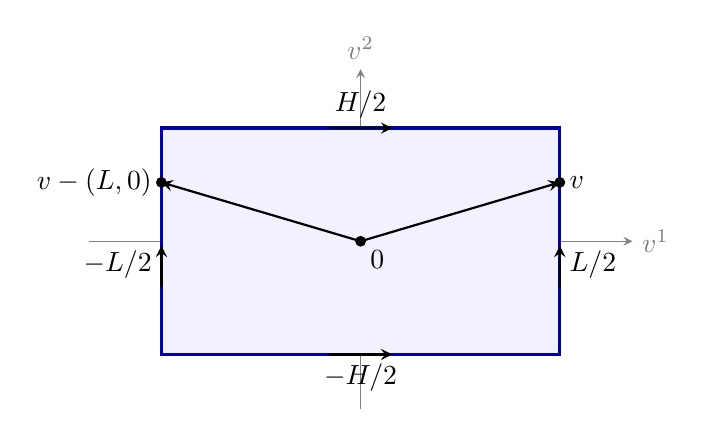
\begin{tikzpicture}[scale=1.15,>=stealth]
	\draw[->,gray] (-3.0,0)--(3.0,0) node[right] {\(v^1\)};
	\draw[->,gray] (0,-1.85)--(0,1.9) node[above] {\(v^2\)};
	\fill[blue!5] (-2.2,-1.25) rectangle (2.2,1.25);
	\draw[very thick,blue!65!black] (-2.2,-1.25) rectangle (2.2,1.25);
	\draw[thick,->] (0,0)--(2.2,0.65);
	\draw[thick,->] (0,0)--(-2.2,0.65);
	\fill (0,0) circle (1.7pt) node[below right] {\(0\)};
	\fill (2.2,0.65) circle (1.7pt) node[right] {\(v\)};
	\fill (-2.2,0.65) circle (1.7pt) node[left] {\(v-(L,0)\)};
	\node[below] at (0,-1.25) {\(-H/2\)};
	\node[above] at (0,1.25) {\(H/2\)};
	\node[below right] at (2.2,0) {\(L/2\)};
	\node[below left] at (-2.2,0) {\(-L/2\)};
	\draw[->,thick] (-0.35,1.25)--(0.35,1.25);
	\draw[->,thick] (-0.35,-1.25)--(0.35,-1.25);
	\draw[->,thick] (2.2,-0.5)--(2.2,-0.05);
	\draw[->,thick] (-2.2,-0.5)--(-2.2,-0.05);
\end{tikzpicture}

	\caption[矩形平坦环面的割迹]{矩形平坦环面的割迹。取格 \(L\mathbb Z\times H\mathbb Z\)，图中矩形为原点的最近点区域 \([-L/2,L/2]\times[-H/2,H/2]\)。相对边在商中识别，整条边界的像组成基点的割迹；边中点有两条最短线，角点有四条。}
	\label{g3:fig:torus-cut-locus}
\end{figure}

覆盖空间也能用来计算其他商度量。下面先把所需的距离公式和完备性传递写清楚。

\begin{proposition}[黎曼覆盖的距离公式]\label{g3:prop:riemannian-covering-distance}
	设 \(\pi:(\widetilde M,\widetilde g)\to(M,g)\) 是连通无边界黎曼流形之间的覆盖，且每点附近的限制是等距映射。若 \(\widetilde M\) 完备，则 \(M\) 完备。对固定提升 \(\widetilde p\in\pi^{-1}(p)\)，有
	\[
		d_M(p,q)=\min_{\widetilde q\in\pi^{-1}(q)}
		d_{\widetilde M}(\widetilde p,\widetilde q).
	\]
	若覆盖来自等距变换群 \(\Gamma\) 的自由作用且纤维正是其轨道，右边等于 \(\min_{\gamma\in\Gamma}d_{\widetilde M}(\widetilde p,\gamma\widetilde q_0)\)，其中 \(\widetilde q_0\) 是任一固定提升。
\end{proposition}
\begin{proof}
	局部等距保持 Levi-Civita 联络：将一个联络通过局部等距搬运，仍满足度量相容和无挠，由唯一性就是另一侧的 Levi-Civita 联络。因此它保持测地线与长度。给定 \(M\) 上的测地线初值，在 \(\widetilde M\) 选取对应初值，所得全时测地线投影后就是原初值的全时解。故 \(M\) 测地完备，再由 Hopf--Rinow 定理得到度量完备。

	在 \(M\) 上取从 \(p\) 到 \(q\) 的最短测地线，从 \(\widetilde p\) 将其提升，终点记为 \(\widetilde q\)。提升长度仍为 \(d_M(p,q)\)，所以 \(d_{\widetilde M}(\widetilde p,\widetilde q)\le d_M(p,q)\)。反向不等式对任意提升终点都成立，因为连接提升端点的曲线投影后长度不变。两者合并，既得到等式，也证明最小值取得。轨道表述只是把纤维中的点重新标记。
\end{proof}

\begin{example}[实射影空间]\label{g3:exm:projective-cut-locus}
	令 \(\mathbb{RP}^n=S_a^n/\{p\sim-p\}\)，取使商映射局部等距的度量。反极点作用自由，足够小的球与其反极点球不交，所以商映射是二重覆盖。令 \(\theta=\arccos(\langle p,q\rangle/a^2)\)，上一命题给出
	\[
		d([p],[q])=a\min\{\theta,\pi-\theta\}
		=a\arccos\frac{|\langle p,q\rangle|}{a^2}.
	\]
	从 \([p]\) 出发的单位速测地线提升为从 \(p\) 出发的大圆；它在 \(t\le\pi a/2\) 时最短，随后一段时间选取反极点提升更短。因此每个方向的割时为 \(\pi a/2\)，割迹为赤道 \(\{q:\langle p,q\rangle=0\}\) 在商中的像，即嵌入的 \(\mathbb{RP}^{n-1}\)。在半径 \(\pi a/2\) 的开切球上，球面指数映射的像是以 \(p\) 为中心的开半球，它与自身的反极点像不交，故商后的指数映射是微分同胚。任意更大的切球内，\((\pi a/2)u\) 与 \(-(\pi a/2)u\) 的像相同，故
	\[
		\operatorname{inj}(\mathbb{RP}^n)=\pi a/2.
	\]
\end{example}

球面在一个点处汇集所有割方向，矩形平坦环面把最近点区域的边界粘成图形，实射影空间则出现整个射影超平面。这些差别来自指数映射的全局行为；点附近总能建立法坐标，并不能决定较远处最短线的条数。
% 纲要条目排为编号小节标题，并进入目录与书签；说明段仍保留于纲要注释中。


\begin{chaptersummary}
	测地线由初始位置和速度唯一确定，速度长度恒定。指数映射把初速度变成时间一的终点；其零处微分为恒等映射，所以零向量附近有法坐标。Gauss 引理进一步说明径向与角向变化正交，从而给出径向线的长度下界及等号条件。出界曲线也必须先付出足够的长度，这使局部计算能够与流形中的所有竞争曲线比较。

	\ProseParagraphBreak

	曲线长度的下确界是与流形拓扑一致的距离。双端点指数映射提供统一的短线，坐标平方函数沿短测地线的凸性则给出强凸邻域。最短曲线不能有角点，按弧长参数化后必为测地线；反过来，一条测地线延长后可能不再最短。

	\ProseParagraphBreak

	Hopf--Rinow 定理把度量完备、所有测地线全时存在、某个基点的指数映射全域定义，以及闭有界集紧性连成等价闭环。完备性还保证任意两点之间存在最短测地线。割时记录这种极小性沿某个方向能保持多久；割时之前的最短线唯一，有限割时处则出现多条最短线或指数映射微分退化。注入半径给出指数坐标可用的球半径，并在紧集上有统一正下界。球面、平坦环面与实射影空间展示了不同的全局识别方式。
\end{chaptersummary}

\BookExercises

\begin{exercise}\label{g3:ex:exponential-line-incomplete}
	在 \(M=\mathbb R\) 上取度量 \(g=e^{2x}\mathrm{d}x^2\)。
	\begin{enumerate}
		\item 证明 \(F(x)=e^x\) 是到 Euclid 半直线 \((0,\infty)\) 的等距微分同胚，并求内在距离 \(d_g(p,q)\)。
		\item 对初值 \(\gamma(0)=p\)、\(\dot\gamma(0)=v\partial_x|_p\)，求最大测地线及其定义区间，进而求 \(\exp_p\) 的定义域和表达式。
		\item 按\cref{g3:def:injectivity-radius}计算 \(\operatorname{inj}_g(p)\)，并证明此流形不完备。
	\end{enumerate}
\end{exercise}
\begin{solution}
	1. \(F\) 是 \(\mathbb R\) 到 \((0,\infty)\) 的光滑双射，其逆为对数函数，且
	\[
		F^*(\mathrm{d}y^2)=(e^x\mathrm{d}x)^2=g.
	\]
	因此它保持曲线长度。半直线内任意连接 \(e^p,e^q\) 的曲线长度至少为 \(|e^q-e^p|\)，连接端点的直线段仍在半直线内并达到这个下界，故
	\[
		d_g(p,q)=|e^q-e^p|.
	\]

	2. 在坐标 \(y=F(x)\) 中，测地线方程是 \(\ddot y=0\)。初速度变为 \(\dot y(0)=e^pv\)，所以
	\[
		y(t)=e^p(1+vt),\qquad
		\gamma(t)=p+\log(1+vt).
	\]
	允许的最大时间区间由 \(1+vt>0\) 决定：
	\[
		I_{p,v}=
		\begin{cases}
			(-1/v,\infty),&v>0,\\
			\mathbb R,&v=0,\\
			(-\infty,-1/v),&v<0.
		\end{cases}
	\]
	有限端点处 \(y(t)\to0\)，对应 \(\gamma(t)\to-\infty\)，没有流形内的延拓点。时间一可取当且仅当 \(v>-1\)，故
	\[
		\mathcal E_p=\{v\partial_x|_p:v>-1\},\qquad
		\exp_p(v\partial_x|_p)=p+\log(1+v).
	\]

	3. 切向量的度量长度为 \(g_p(v\partial_x,v\partial_x)^{1/2}=e^p|v|\)，因而半径 \(r\) 的切球对应区间 \((-re^{-p},re^{-p})\)。当 \(0<r\le e^p\) 时，这个开区间包含于 \(v>-1\)，且指数映射的导数 \(1/(1+v)\) 为正，故指数映射在该球上为微分同胚。若 \(r>e^p\)，切球包含 \(v=-1\)，指数映射在此没有定义。因此
	\[
		\operatorname{inj}_g(p)=e^p.
	\]
	序列 \(p_j=-j\) 关于 \(d_g\) 为 Cauchy 序列，因为 \(F(p_j)=e^{-j}\to0\)；它在 \(M\) 中没有极限。也可以取 \(v=-1\)，得到在时间一终止的最大测地线。这分别检验了度量不完备和测地不完备。
\end{solution}

\begin{exercise}\label{g3:ex:complete-product-distance-injectivity}
	设 \((M,g)\)、\((N,h)\) 为连通、无边界的完备光滑黎曼流形，乘积上取度量 \(G=g\oplus h\)。证明
	\[
		d_G((p,q),(p',q'))^2=d_g(p,p')^2+d_h(q,q')^2,
	\]
	并证明 \(M\times N\) 完备。求乘积的指数映射，再按定义证明
	\[
		\operatorname{inj}_G(p,q)
		=\min\{\operatorname{inj}_g(p),\operatorname{inj}_h(q)\},
	\]
	其中允许半径为无穷。
\end{exercise}
\begin{solution}
	对乘积曲线 \(c=(\alpha,\beta):[0,1]\to M\times N\)，记两个分量的速度长度为 \(a(t),b(t)\)，曲线长度为 \(L_\alpha,L_\beta\)。积分的向量三角不等式给出
	\[
		L_G(c)=\int_0^1\sqrt{a(t)^2+b(t)^2}\,\mathrm{d}t
		\ge\sqrt{L_\alpha^2+L_\beta^2}
		\ge\sqrt{d_g(p,p')^2+d_h(q,q')^2}.
	\]
	第一处不等式也可直接检验：若 \((L_\alpha,L_\beta)\ne(0,0)\)，将 \((a(t),b(t))\) 与其积分向量的单位方向作内积，再逐点用内积不等式，积分即可。零向量情形直接成立。

	由\cref{g3:thm:hopf-rinow}，两个因子中均存在实现端点距离的测地线。将它们都参数化在 \([0,1]\) 上，使速度长度分别恒为 \(d_g(p,p')\)、\(d_h(q,q')\)；距离为零的因子取常曲线。它们组成的乘积曲线速度长度恒为这两个数的平方和开根，达到上述下界。因此距离公式成立。乘积中的 Cauchy 序列投影到两个因子后仍是 Cauchy 序列，各有极限；距离公式又说明乘积序列收敛到两极限组成的点，故乘积完备。

	由\cref{g3:prop:product-connection}，乘积测地线方程分成两个因子的测地线方程，初值唯一性给出
	\[
		\exp^G_{(p,q)}(v,w)
		=(\exp^g_pv,\exp^h_qw),\qquad
		|(v,w)|_G^2=|v|_g^2+|w|_h^2.
	\]
	完备性保证这些指数映射处处有定义。若 \(r\) 小于两个因子的注入半径，则各指数映射在半径 \(r\) 的切球上都是微分同胚，它们的乘积在两个切球的乘积上也是微分同胚。半径 \(r\) 的乘积切球是其中的开子集，故限制后仍为微分同胚，得到所求等式的“\(\ge\)”方向。

	反过来，若乘积指数映射在半径 \(r\) 的切球上为微分同胚，则限制到 \((v,0)\)、\(|v|_g<r\)，可知 \(\exp_p^g\) 在 \(B_p(0,r)\) 上单射。同时
	\[
		\mathrm{d}\exp^G_{(p,q)}\big|_{(v,0)}
		=\operatorname{diag}\bigl((\mathrm{d}\exp^g_p)_v,
			(\mathrm{d}\exp^h_q)_0\bigr)
	\]
	可逆，且第二块为恒等，所以第一块可逆。于是 \(\exp_p^g\) 是单射的局部微分同胚，其局部光滑逆拼成像上的光滑逆；它在整个 \(B_p(0,r)\) 上为微分同胚。交换两个因子，得到同样的结论。故任意乘积可用半径都是两个因子各自的可用半径，对上确界取值即得“\(\le\)”方向，也包括无穷半径的情形。
\end{solution}

\begin{exercise}\label{g3:ex:complete-metric-lower-bound}
	设 \(g,h\) 是同一连通、无边界光滑流形 \(M\) 上的黎曼度量，且 \((M,g)\) 完备。
	\begin{enumerate}
		\item 若存在常数 \(c>0\)，使 \(h(\xi,\xi)\ge c^2g(\xi,\xi)\) 对一切切向量成立，证明 \((M,h)\) 完备。说明仅有距离下界以后，还需怎样把 \(g\) 意义下的极限变成 \(h\) 意义下的极限。
		\item 证明全局上界 \(h\le C^2g\) 不能替代这一假设。可在 \(\mathbb R\) 上取
		\[
			g=\mathrm{d}x^2,\qquad
			h=e^{-2\sqrt{1+x^2}}\mathrm{d}x^2.
		\]
	\end{enumerate}
\end{exercise}
\begin{solution}
	1. 对每条分片光滑曲线积分速度下界，得到 \(L_h\ge cL_g\)，继而
	\[
		d_h(x,y)\ge c\,d_g(x,y).
	\]
	所以 \(h\)-Cauchy 序列 \((p_j)\) 也是 \(g\)-Cauchy 序列。由 \(g\) 完备，存在 \(p\in M\)，使 \(d_g(p_j,p)\to0\)。\cref{g3:thm:riemannian-distance}说明 \(p_j\) 在流形拓扑中也趋于 \(p\)。

	取以 \(p\) 为原点的坐标图，并在其中取闭包紧含于图域的坐标球。度量 \(h\) 的系数在这个闭球上有界，因此存在 \(A>0\)，使 \(h_{ab}(x)\xi^a\xi^b\le A^2|\xi|^2\)。充分大的 \(j\) 位于较小坐标球中，将 \(p_j\) 与 \(p\) 用坐标直线段连接，便有
	\[
		d_h(p_j,p)\le A\,|x(p_j)-x(p)|\longrightarrow0.
	\]
	这一步只在极限点附近使用度量上界；全局不要求 \(h\) 被 \(g\) 的常数倍控制。由此每个 \(h\)-Cauchy 序列都收敛，故 \(h\) 完备。

	2. 所给度量光滑正定，且 \(h\le g\)。令
	\[
		F(x)=\int_0^x e^{-\sqrt{1+s^2}}\,\mathrm{d}s,\qquad
		A=\int_0^\infty e^{-\sqrt{1+s^2}}\,\mathrm{d}s.
	\]
	因 \(\sqrt{1+s^2}\ge s\) 对 \(s\ge0\) 成立，有 \(0<A\le1\)。\(F'\) 处处为正，且被积函数为偶函数，所以 \(F\) 是到有限开区间 \((-A,A)\) 的微分同胚，满足 \(F^*(\mathrm{d}y^2)=h\)。因此
	\[
		d_h(x,y)=|F(x)-F(y)|.
	\]
	序列 \(x_j=j\) 映到趋于 \(A\) 的序列，是 \(h\)-Cauchy 序列，却没有流形内的极限。缩小远处的长度尺度可以使通往无穷远的路径具有有限长度，因此全局上界 \(h\le g\) 不能保证完备性。
\end{solution}

\begin{exercise}\label{g3:ex:squared-distance-at-center}
	设 \((M,g)\) 为无边界光滑黎曼流形，\(p\in M\)、\(R>0\)，\(\exp_p:B_p(0,R)\to U_R\) 为微分同胚，令 \(r(q)=d_g(p,q)\)。证明 \(r\) 在 \(U_R\setminus\{p\}\) 上光滑，并求其梯度，证明 \(|\operatorname{grad}_g r|_g=1\)。再证明 \(f=r^2\) 在整个 \(U_R\) 上光滑，且
	\[
		(H_f)_p=2g_p.
	\]
	这里 \(\nabla\) 为 \(g\) 的 Levi-Civita 联络，沿用协变二阶导数的定义
	\[
		H_f(X,Y)=X(Yf)-(\nabla_XY)f.
	\]
\end{exercise}
\begin{solution}
	由\cref{g3:prop:normal-radial-minimality}，若 \(q=\exp_p(v)\)，则 \(r(q)=|v|_g\)。因此 \(r\) 在去掉中心的法邻域中光滑。固定非零 \(v\)，令 \(u=v/|v|_g\)。对任意 \(w\in\mathrm{T}_pM\)，有
	\[
		\mathrm{d}r_q\bigl((\mathrm{d}\exp_p)_vw\bigr)
		=\frac{g_p(v,w)}{|v|_g}.
	\]
	Gauss 引理把右端改写为
	\[
		g_q\bigl((\mathrm{d}\exp_p)_vu,(\mathrm{d}\exp_p)_vw\bigr).
	\]
	由于 \((\mathrm{d}\exp_p)_v\) 可逆，这对 \(q\) 处的全部切向量确定了梯度：
	\[
		\operatorname{grad}_g r\big|_q=(\mathrm{d}\exp_p)_vu=\partial_r|_q,
		\qquad |\operatorname{grad}_g r|_g=1.
	\]

	取由 \(\mathrm{T}_pM\) 的正交单位基得到的法坐标，则
	\[
		f(x)=r(x)^2=\sum_i(x^i)^2.
	\]
	此表达在中心也光滑，且 \(\mathrm{d}f_p=0\)。由 \(H_f\) 的定义直接得到坐标分量
	\[
		(H_f)_{ij}=\partial_i\partial_jf-\Gamma^k_{ij}\partial_kf.
	\]
	在 \(p\) 处第二项为零，第一项是 \(2\delta_{ij}\)。又 \(g_{ij}(p)=\delta_{ij}\)，故 \((H_f)_p=2g_p\)。距离函数本身在中心有绝对值型行为，平方则消除了这一不可微点。
\end{solution}

\begin{exercise}\label{g3:ex:completeness-escaping-curves}
	设 \((M,g)\) 为连通、无边界光滑黎曼流形。称连续曲线 \(c:[0,b)\to M\)、\(0<b\le\infty\)，在 \(t\uparrow b\) 时离开所有紧集，是指对每个紧集 \(K\subset M\)，都存在 \(t_K<b\)，使 \(c(t)\notin K\) 对 \(t_K<t<b\) 成立。假设曲线在每个紧参数子区间上分片光滑，并定义
	\[
		L_g(c)=\sup_{0<T<b}L_g(c|_{[0,T]}).
	\]
	证明：\(M\) 完备，当且仅当每条离开所有紧集的这种曲线都有无限长度。反向证明中，可使用有限端点的最大测地线，但须证明其位置确实离开所有紧集。
\end{exercise}
\begin{solution}
	先设 \(M\) 完备。若某条曲线的总长度为有限数 \(L\)，则对所有 \(t<b\)，
	\[
		d_g(c(0),c(t))\le L.
	\]
	由 Hopf--Rinow 定理，闭距离球 \(\overline B_{d_g}(c(0),L)\) 紧，而整条曲线都在其中。因此它不能离开所有紧集，证明一个方向。

	反过来，若 \(M\) 不完备，Hopf--Rinow 定理给出一条不能全时延拓的最大测地线。必要时反向并作仿射重参数化，可取单位速测地线 \(\gamma:[0,b)\to M\)，其中 \(b<\infty\) 是其最大右端点。它的长度为 \(b\)。下面证明它离开所有紧集。

	若存在紧集 \(K\) 和时刻 \(t_j\uparrow b\)，使 \(\gamma(t_j)\in K\)，取子列可使 \(\gamma(t_j)\to q\in K\)。因速度为一，当 \(t<t_j\) 时有
	\[
		d_g(\gamma(t),\gamma(t_j))\le t_j-t.
	\]
	让 \(j\to\infty\)，得到 \(d_g(\gamma(t),q)\le b-t\)，所以整个曲线尾部趋于 \(q\)。这里从反复进入紧集到存在位置极限，使用了有限剩余长度；仅知道测地线的某些位置有收敛子列尚不足以直接给出二阶方程的初值。

	在 \(q\) 附近取闭包紧含于一个坐标图的邻域，曲线尾部最终留在其中。度量矩阵有统一正下界，因此单位速条件使坐标速度 \(\dot x(t)\) 有界；Christoffel 系数也有界，由
	\[
		\ddot x^k=-\Gamma^k_{ij}(x)\dot x^i\dot x^j
	\]
	可知坐标加速度有界。于是 \(\dot x(t)\) 在 \(t\uparrow b\) 时有极限 \(w\)，并且 \((x(t),\dot x(t))\to(x(q),w)\)。测地线一阶系统的积分形式延续到 \(b\)；以 \((q,w)\) 为初值应用\cref{g3:thm:geodesic-ivp}，便将原解延长到 \(b\) 之后，违背最大性。因此每个紧集都只能在某个末时刻以前被访问，\(\gamma\) 确实离开所有紧集。它具有有限长度，与题设性质矛盾，故该性质推出完备。
\end{solution}

\begin{exercise}\label{g3:ex:sphere-normal-volume}
	在半径 \(a>0\) 的圆球面 \(S_a^n\subset\mathbb R^{n+1}\)、\(n\ge1\) 上，固定 \(p\) 并使用由 \(\mathrm{T}_pS_a^n\) 的正交单位基产生的法坐标。设 \(v=ru\)、\(0<r<\pi a\)、\(|u|=1\)。直接对式\eqref{g3:eq:round-sphere-exponential}求微分，证明 \(\exp_p\) 在径向上的长度倍率为 \(1\)，在与 \(v\) 正交的方向上的长度倍率为
	\[
		s(r)=\frac{\sin(r/a)}{r/a}.
	\]
	由此求法坐标中的度量矩阵及体积密度，并说明其在中心的延拓。
\end{exercise}
\begin{solution}
	对任意 \(w\in\mathrm{T}_pS_a^n\)，写
	\[
		w=\lambda u+w_\perp,\qquad
		\lambda=\langle u,w\rangle,\quad w_\perp\perp u.
	\]
	因为 \(\mathrm{d}r_v(w)=\lambda\)、\(\mathrm{d}u_v(w)=w_\perp/r\)，对
	\[
		\exp_p(v)=\cos(r/a)p+a\sin(r/a)u
	\]
	求微分得到
	\[
		(\mathrm{d}\exp_p)_vw
		=\lambda E_r+s(r)w_\perp,\qquad
		E_r=-\frac{\sin(r/a)}a\,p+\cos(r/a)u.
	\]
	向量 \(E_r\) 的环境长度为一，并且与 \(w_\perp\) 正交；两者都切于终点球面。因此
	\[
		\left|(\mathrm{d}\exp_p)_vw\right|_g^2
		=\lambda^2+s(r)^2|w_\perp|^2,
	\]
	给出两种所求倍率。这个计算还直接验证了 Gauss 引理中的径向正交性。

	在固定正交单位基中写 \(v=(x^1,\ldots,x^n)\)，则 \(r^2=\sum_i(x^i)^2\)，拉回度量矩阵为
	\[
		g_{ij}(x)=s(r)^2\delta_{ij}
		+\bigl(1-s(r)^2\bigr)\frac{x^ix^j}{r^2}.
	\]
	径向特征值为 \(1\)，其余 \(n-1\) 个特征值为 \(s(r)^2\)。在 \(0<r<\pi a\) 内，\(s(r)>0\)，所以
	\[
		\sqrt{\det(g_{ij}(x))}
		=s(r)^{n-1},\qquad
		\mu_g=
		\left(\frac{\sin(r/a)}{r/a}\right)^{n-1}
		\left|\mathrm{d}x^1\cdots\mathrm{d}x^n\right|.
	\]
	当 \(n=1\) 时没有横向方向，密度系数为 \(1\)，与此公式一致。

	最后，\(\sin z/z\) 在 \(z=0\) 的值取 \(1\) 后，是 \(z^2\) 的光滑函数。因而 \(s(r)\) 是 \(r^2\) 的光滑函数，且
	\[
		s(r)^2=1-\frac{r^2}{3a^2}+O(r^4).
	\]
	于是 \((1-s(r)^2)/r^2\) 在零处光滑延拓，取值为 \(1/(3a^2)\)；度量矩阵在中心延拓为 \(\delta_{ij}\)，体积密度系数光滑延拓为 \(1\)。以上计算直接使用显式指数映射，给出了正曲率球面相对于切空间 Euclid 体积的局部变化。
\end{solution}

\begin{exercise}\label{g3:ex:rectangular-torus-distance}
	设 \(T=\mathbb R^2/(L\mathbb Z\times H\mathbb Z)\)，其中 \(L,H>0\)，取平坦商度量。计算其直径、注入半径，以及从原点类到任意一点的最短测地线条数。再考虑平坦圆柱 \(C=\mathbb R\times(\mathbb R/L\mathbb Z)\)，求原点类的割迹和单位方向 \(u=(u_1,u_2)\) 的割时。
\end{exercise}
\begin{solution}
	每个点类都有代表 \((x,y)\in[-L/2,L/2]\times[-H/2,H/2]\)。由式\eqref{g3:eq:flat-torus-distance}，到原点类的距离为 \(\sqrt{x^2+y^2}\)，故最大值在角点取得，为 \(\tfrac12\sqrt{L^2+H^2}\)。平移是等距映射，所以任意点对的距离也不超过此值，从而
	\[
		\operatorname{diam}(T)=\tfrac12\sqrt{L^2+H^2},\qquad
		\operatorname{inj}(T)=\tfrac12\min\{L,H\}.
	\]
	最近代表在每个坐标方向独立选择：若 \(|x|<L/2\)，第一个坐标唯一；若 \(|x|=L/2\)，两个符号都可选。第二个坐标同理。因此最近点区域内部的点有一条最短线，边的内部有两条，四角共同代表的点有四条。从基点到自身，最短线只有常值曲线。每个最近代表给出一个直线段，其投影的初速度不同，故这些线确实互不相同；任意最短线提升后又必须是到某个最近代表的直线段，所以没有遗漏。

	圆柱只在第二坐标上取商，距离公式为
	\[
		d_C([0,0],[x,y])=\min_{k\in\mathbb Z}\sqrt{x^2+(y+kL)^2}.
	\]
	最近点区域是无限条带 \(|y|\le L/2\)，两条边界在商中识别，故原点类的割迹为直线 \(\{[x,L/2]:x\in\mathbb R\}\)。沿方向 \(u\) 的线最短恰好到第一次抵达该边界，因此
	\[
		c_p(u)=
		\begin{cases}
			L/(2|u_2|),&u_2\ne0,\\
			\infty,&u_2=0.
		\end{cases}
	\]
	相应注入半径为 \(L/2\)。同一个完备流形上，可以有永远最短的方向，也可以有有限割时的方向。
\end{solution}

\begin{exercise}\label{g3:ex:complete-cusp-zero-injectivity}
	设 \((M,g)\) 为连通、完备、无边界的光滑黎曼流形，\(p\in M\)。
	\begin{enumerate}
		\item 若基于 \(p\) 的分片光滑环路 \(\alpha\) 不能在 \(M\) 中收缩为常值环路，证明 \(\operatorname{inj}_g(p)\le L_g(\alpha)/2\)。
		\item 在圆柱 \(M=\mathbb R\times(\mathbb R/2\pi\mathbb Z)\) 上取
		\[
			g=\mathrm dr^2+e^{-2r}\mathrm d\theta^2.
		\]
		证明它完备，但 \(\operatorname{inj}_g(M)=0\)。
	\end{enumerate}
\end{exercise}
\begin{solution}
	1. 记 \(\ell=L_g(\alpha)\)。沿环路的正向和反向两段都能连接 \(p\) 与任意一点 \(q\)，其中较短的一段长至多 \(\ell/2\)，所以整条环路位于 \(\overline B_d(p,\ell/2)\)。若 \(\ell/2<\operatorname{inj}_g(p)\)，取
	\[
		\ell/2<\rho<\operatorname{inj}_g(p).
	\]
	由\cref{g3:prop:compact-injectivity-lower-bound}，\(B_d(p,\rho)=\exp_p B_p(0,\rho)\)，且指数映射是微分同胚。于是
	\[
		H(s,t)=\exp_p\bigl((1-s)\exp_p^{-1}\alpha(t)\bigr)
	\]
	在固定基点的条件下把 \(\alpha\) 收缩为常值环路，矛盾。

	2. 对任意连接曲线，都有 \(L_g\ge\int|\dot r|\)，因此 \(|r-r'|\le d_g((r,\theta),(r',\theta'))\)。若 \((r_j,\theta_j)\) 为 Cauchy 序列，\(r_j\) 为实数 Cauchy 序列，特别地全部落在某个有界闭区间 \([A,B]\) 中。拓扑圆柱带 \([A,B]\times S^1\) 紧，故该序列有子列在流形拓扑中收敛；距离拓扑相同，所以此子列也在 \(d_g\) 下收敛。Cauchy 性再使整个序列收敛，证明完备。

	基于 \(p_r=(r,0)\) 的圆周环路 \(\alpha_r(t)=(r,2\pi t)\) 长为 \(2\pi e^{-r}\)，且不可收缩。事实上，若它可收缩，投影到第二因子就会把圆周绕行一周的环路收缩；在覆盖 \(\mathbb R\to S^1\)、\(s\mapsto e^{is}\) 下，该环路从零出发的提升终止于 \(2\pi\)，而常值环路的提升终止于零，与第一卷第5.3节的定端点同伦提升结论矛盾。由第一问，
	\[
		0<\operatorname{inj}_g(p_r)\le\pi e^{-r}.
	\]
	令 \(r\to+\infty\)，得到整体下确界为零。各点的注入半径仍为正，趋于零发生在离开所有紧集的过程中。
\end{solution}

\begin{exercise}\label{g3:ex:covering-completeness-converse}
	设 \(\pi:(\widetilde M,\widetilde g)\to(M,g)\) 是连通无边界黎曼流形之间的覆盖，且处处局部等距。证明 \(M\) 完备当且仅当 \(\widetilde M\) 完备。给出一个局部等距映射，说明删去覆盖条件后，从目标完备不能推出源完备。
\end{exercise}
\begin{solution}
	从源完备推出目标完备已由\cref{g3:prop:riemannian-covering-distance}证明。反过来设 \(M\) 完备，给定 \(\widetilde M\) 上的初值 \((\widetilde p,\widetilde v)\)。将其投影到 \(M\)，所得测地线 \(\gamma\) 定义在整个实轴上。对每个正整数 \(N\)，在 \([-N,N]\) 上从 \(t=0\) 分别向正负方向提升 \(\gamma\)，初点指定为 \(\widetilde p\)。道路提升唯一性保证不同 \(N\) 的提升在公共区间相等，因而拼成 \(\mathbb R\) 上的一条提升 \(\widetilde\gamma\)。局部覆盖逆为等距映射，所以提升光滑，并保持测地线方程；其初速度就是 \(\widetilde v\)。由此全部测地线初值全时可解，Hopf--Rinow 定理给出 \(\widetilde M\) 完备。

	带普通度量的包含映射 \((0,1)\hookrightarrow\mathbb R\) 局部等距，但目标完备而源不完备。有限时间内，源中的直线可以到达被删去的端点；该映射不是到 \(\mathbb R\) 的覆盖，不能对全时的目标直线作所需提升。
\end{solution}

\begin{exercise}\label{g3:ex:noncompact-complete-ray}
	设 \((M,g)\) 连通、完备、无边界且非紧。证明对任意 \(p\in M\)，存在单位速测地线 \(\gamma:[0,\infty)\to M\)，满足
	\[
		d(\gamma(s),\gamma(t))=t-s\qquad(0\le s\le t).
	\]
	这样的曲线称为从 \(p\) 出发的测地射线。由此证明至少存在一个 \(u\in S_pM\)，使 \(c_p(u)=\infty\)。
\end{exercise}
\begin{solution}
	由 Hopf--Rinow 定理，有限半径闭球紧。若 \(d(p,\cdot)\) 有上界，整个流形就是一个紧闭球，与非紧性矛盾。因此可选 \(q_j\)，使 \(\ell_j=d(p,q_j)\to\infty\)。取从 \(p\) 到 \(q_j\) 的单位速最短测地线，初方向记为 \(u_j\in S_pM\)。有限维单位球面紧，故取子列可使 \(u_j\to u\)。完备性保证 \(\gamma(t)=\exp_p(tu)\) 对所有 \(t\ge0\) 有定义。

	固定 \(0\le s\le t\)。充分大的 \(j\) 有 \(\ell_j\ge t\)，最短线的子段仍最短，故
	\[
		d(\exp_p(su_j),\exp_p(tu_j))=t-s.
	\]
	指数映射和距离均连续，令 \(j\to\infty\) 得到所求等式。取 \(s=0\)，可见从 \(p\) 到 \(\gamma(t)\) 的线段对每个 \(t\) 都最短，所以 \(c_p(u)=\infty\)。
\end{solution}

\begin{exercise}\label{g3:ex:isometry-first-jet}
	设 \(F:(M,g)\to(N,h)\) 为黎曼等距同构，即满足 \(F^*h=g\) 的微分同胚。证明在指数映射有定义处，
	\[
		F(\exp_pv)=\exp_{F(p)}((\mathrm dF)_pv).
	\]
	若 \(M\) 还连通、完备，证明 \(F\) 由一点处的值 \(F(p)\) 及微分 \((\mathrm dF)_p\) 唯一确定。并证明
	\[
		F(\operatorname{Cut}_M(p))=\operatorname{Cut}_N(F(p)),\qquad
		\operatorname{inj}_h(F(p))=\operatorname{inj}_g(p).
	\]
\end{exercise}
\begin{solution}
	将 \(M\) 上的联络通过 \(F\) 搬到 \(N\)，度量相容和无挠性质保持成立，所以它由 Levi-Civita 唯一性就是 \(N\) 上的联络。因此 \(F\circ\gamma_{p,v}\) 是初值 \((F(p),(\mathrm dF)_pv)\) 的测地线。初值唯一性给出全时间的对应，取时间一即得指数映射公式。

	若另一个等距同构 \(G:M\to N\) 在 \(p\) 处有同样的值与微分，则对每个 \(v\in\mathrm T_pM\)，有 \(F(\exp_pv)=G(\exp_pv)\)。Hopf--Rinow 定理使 \(\exp_p\) 满射，所以 \(F=G\) 于整个 \(M\)。

	等距同构保持全部曲线长度与端点距离，其微分把单位切球面等距地对应起来。因此
	\[
		c_{F(p)}((\mathrm dF)_pu)=c_p(u),
	\]
	并把有限割时的终点一一对应，得到割迹等式。指数映射公式还说明，两侧指数映射分别通过线性等距同构 \((\mathrm dF)_p\) 和微分同胚 \(F\) 共轭，所以使指数映射在切球上成为微分同胚的半径完全相同，注入半径相等。
\end{solution}

\begin{exercise}\label{g3:ex:scaling-cut-injectivity}
	设 \((M,g)\) 连通、完备、无边界，\(a>0\)，令 \(\widetilde g=a^2g\)。比较两种度量的距离、指数映射、割迹、割时及注入半径。写出割时公式时，明确两侧单位初方向的对应。
\end{exercise}
\begin{solution}
	每条曲线的长度乘以 \(a\)，取下确界得到 \(d_{\widetilde g}=a\,d_g\)，所以完备性保持不变。上一章的常数缩放计算说明两种度量的 Levi-Civita 联络相同，故同一个切向量给出同一个带参数测地线，指数映射也相同。

	若 \(|u|_g=1\)，则 \(|u/a|_{\widetilde g}=1\)，且
	\[
		d_{\widetilde g}\bigl(p,\exp_p(tu/a)\bigr)
		=a\,d_g\bigl(p,\exp_p((t/a)u)\bigr).
	\]
	左边等于 \(t\)，当且仅当右侧原距离等于 \(t/a\)。因此
	\[
		c_p^{\widetilde g}(u/a)=a\,c_p^g(u).
	\]
	达到有限割时的向量相同：\((a c_p^g(u))(u/a)=c_p^g(u)u\)，所以割迹作为点集不变。最后，\(\widetilde g\) 的半径 \(r\) 切球就是 \(g\) 的半径 \(r/a\) 切球，指数映射本身不变，故
	\[
		\operatorname{inj}_{\widetilde g}(p)=a\,\operatorname{inj}_g(p),\qquad
		\operatorname{inj}_{\widetilde g}(M)=a\,\operatorname{inj}_g(M).
	\]
\end{solution}

% !TeX root = ../../Book3.tex
% 纲要标题：## 第3章　曲率张量与法坐标展开
% 纲要位置：几何学计划纲要.md，第 2192 行。
% 正文状态：初稿；尚未正式审核。

% 纲要内容开始
% 
% > 本章目标与证明范围：从协变微分的非交换性得到代数曲率张量，再把各次收缩和法坐标展开联系到可观测的长度、面积和体积变化。
% 
% 纲要内容结束

\chapter{曲率张量与法坐标展开}
\label{g3:ch:03}
\BookChapterNumber{g3:ch:03}

\begin{chapterabstract}
	法坐标消去度量在中心的一阶变化，二阶变化则由曲率控制。本章从协变微分的非交换性证明曲率的张量性、代数对称性及两条 Bianchi 恒等式，建立曲率算子、截面曲率、Ricci 曲率与标量曲率之间的关系。随后推导联络、度量和体积密度的法坐标展开，把不同收缩解释为长度、面积和小球体积的低阶变化。空间形式、乘积、翘曲积与共形度量提供计算模型，Weyl 分解则分离标量、无迹 Ricci 和无迹四阶曲率三部分。
\end{chapterabstract}

\begin{learninggoals}
	\begin{itemize}
		\item 在向量曲率、四阶曲率张量和二向量曲率算子之间转换，并核对指标次序与球面的正曲率符号。
		\item 证明两条 Bianchi 恒等式及其收缩，说明截面、Ricci、标量和曲率算子正性之间的含义与差别。
		\item 从法坐标径向条件求出联络和度量的低阶项，推导体积密度、小球体积及面积的展开，并控制余项。
		\item 计算乘积、翘曲积及共形变化的曲率，使用 Weyl 分解解释低维确定性和高维信息损失。
	\end{itemize}
\end{learninggoals}

在平面上画一个半径很小的圆，它的周长是 \(2\pi r\)。在半径 \(a\) 的球面上，以沿球面的距离 \(r\) 为半径画圆，周长却是 \(2\pi a\sin(r/a)\)。当 \(r\) 很小时，两者的一阶项相同，差异从三次项开始：
\[
	2\pi a\sin(r/a)=2\pi r-\frac{\pi}{3a^2}r^3+O(r^5).
\]
这个差异可以由长度测量得到，不需要先把球面与环境空间中的某个法向比较。高维中，不同二维方向可以出现不同的差异；将它们沿某个方向相加，会得到 Ricci 曲率，再把方向全部平均，则出现标量曲率。

\ProseParagraphBreak

第二章的法坐标使 \(g_{ij}(p)=\delta_{ij}\)、\(\partial_kg_{ij}(p)=0\)。因此我们可以把度量与 Euclid 度量的首个差异集中在二阶项中。证明将沿两个方向进行：先由联络求导的交换差得到曲率，找出它必须满足的对称性；再由这些曲率分量恢复法坐标中的二次项，计算可观测的几何量。曲率约束之间的区别也将在实际局部度量中检验。

\ProseParagraphBreak

本章使用第一章的 Levi-Civita 联络、体积密度及非负 Laplace 算子 \(\Delta_g=-\operatorname{div}_g\operatorname{grad}_g\)，以及第二章的指数映射、Gauss 引理和法坐标。外积空间只需有限维线性代数：\(X\wedge Y\) 表示由两个向量张成的有向面积元素。流形及度量均光滑，通常假设无边界；紧性、连通性和维数限制在实际需要的结果中另行写明。法坐标展开由坐标恒等式和 Taylor 公式推出。

\ProseParagraphBreak

作为阅读对照，曲率、曲率算子及各次收缩可参看 Petersen 第3版第3.1.1--3.1.6节；球面、乘积及旋转型度量见第4.2.1--4.2.3节，共形表示见第4.3.3节，指数坐标性质见第5.5.3节\cite[第3.1.1--3.1.6节; 第4.2.1--4.2.3节; 第4.3.3节; 第5.5.3节]{Petersen2016}。本章固定的四阶张量次序是 \(\mathrm{Rm}(X,Y,Z,W)=g(R(X,Y)W,Z)\)，因此 \(\mathrm{Rm}(u,v,u,v)\) 是正交单位向量所张截面的曲率。

% !TeX root = ../../Book3.tex
% 纲要标题：### 3.1 曲率的代数结构
% 纲要位置：几何学计划纲要.md，第 2196 行。
% 正文状态：初稿；尚未正式审核。

% 纲要内容开始
% 
% * 曲率张量性及符号
% * 四阶张量的对称性
% * 第一、第二 Bianchi 恒等式
% * 曲率算子及二形式上的作用
% 
% 纲要内容结束

\section{曲率的代数结构}
\label{g3:sec:0301}

第一章用联络一形式算出了若干度量的曲率，第二章又在每点建立了使联络系数消失的法坐标。联络系数在一点为零，并不使它们的导数也为零；曲率正从这些导数之间的差别中出现。本节先说明曲率为何只依赖输入向量在一点的值，再把它写成四阶张量，逐一找出由度量相容性和无挠性带来的对称关系。最后将这些分量组织为二向量空间上的自伴算子，使二维截面的曲率与一个有限维线性算子联系起来。

\subsection{曲率张量性及符号}
\label{g3:subsec:0301:01}

对函数而言，两个方向导数的交换子是 Lie 括号：\(X(Yf)-Y(Xf)=[X,Y]f\)。向量场的协变导数还要记录切空间的变化，因而同样减去括号方向的导数后，仍可能留下一个非零项。沿用式\eqref{g3:eq:curvature-definition}的顺序，我们把这个余项作为本章的曲率。

\begin{definition}\label{g3:def:riemann-curvature}
	设 \((M,g)\) 为有限维、无边界光滑黎曼流形，\(\nabla\) 为其 Levi-Civita 联络。对任意光滑向量场 \(X,Y,Z\)，定义
	\[
		R(X,Y)Z
		=\nabla_X\nabla_YZ-\nabla_Y\nabla_XZ-\nabla_{[X,Y]}Z.
	\]
	所得 \(R\) 称为度量 \(g\) 的\term[limanqulvzhangliang]{黎曼曲率张量}[Riemann curvature tensor]。
\end{definition}

第一章已从联络矩阵得到曲率的张量性。下面直接检查联络的乘积规则，说明各导数项为何消去；这一计算对任意光滑线性联络也适用。

\begin{proposition}\label{g3:prop:riemann-curvature-tensorial}
	设 \((M,g)\) 为有限维、无边界光滑黎曼流形。它的曲率 \(R(X,Y)Z\) 对 \(X,Y,Z\) 都为 \(C^\infty(M)\) 线性，并满足 \(R(X,Y)=-R(Y,X)\)。因此每个点 \(p\) 的曲率确定一个交替双线性映射
	\[
		R_p:\mathrm{T}_pM\times\mathrm{T}_pM
		\longrightarrow\operatorname{End}(\mathrm{T}_pM),
	\]
	并随 \(p\) 光滑变化。
\end{proposition}
\begin{proof}
	反对称性由定义直接得到。对光滑函数 \(f\)，由 \([fX,Y]=f[X,Y]-Y(f)X\)，有
	\begin{align*}
		R(fX,Y)Z
		&=f\nabla_X\nabla_YZ-\nabla_Y(f\nabla_XZ)
			-\nabla_{f[X,Y]-Y(f)X}Z\\
		&=fR(X,Y)Z.
	\end{align*}
	两个含 \(Y(f)\nabla_XZ\) 的项相消。第二个输入的函数线性再由反对称性得到。对于第三个输入，先展开
	\[
		\nabla_X\nabla_Y(fZ)
		=X(Yf)Z+(Yf)\nabla_XZ+(Xf)\nabla_YZ
			+f\nabla_X\nabla_YZ.
	\]
	交换 \(X,Y\) 后，中间两项相消；再减去 \(\nabla_{[X,Y]}(fZ)\)，得到
	\[
		R(X,Y)(fZ)
		=fR(X,Y)Z+\bigl(X(Yf)-Y(Xf)-[X,Y]f\bigr)Z
		=fR(X,Y)Z.
	\]
	在局部标架中展开三个输入，函数线性将全部分量移到外面，所以一点处的结果只取决于三个向量在该点的值。联络系数与输入标架光滑，因而输出分量光滑。
\end{proof}

在坐标 \((x^i)\) 中，固定指标顺序
\[
	R(\partial_i,\partial_j)\partial_b
	=R^a{}_{b i j}\partial_a.
\]
其中 \(i,j\) 是求导方向，\(b\) 是被作用的向量指标，\(a\) 是输出指标。由于坐标向量场交换，
\[
	\nabla_{\partial_i}\nabla_{\partial_j}\partial_b
	=\bigl(\partial_i\Gamma^a_{jb}
		+\Gamma^a_{ic}\Gamma^c_{jb}\bigr)\partial_a.
\]
交换 \(i,j\) 并作差，便得到可直接计算的公式
\begin{equation}\label{g3:eq:curvature-coordinate-components}
	R^a{}_{b i j}
	=\partial_i\Gamma^a_{jb}-\partial_j\Gamma^a_{ib}
	+\Gamma^a_{ic}\Gamma^c_{jb}-\Gamma^a_{jc}\Gamma^c_{ib}.
\end{equation}
这与 \(\Omega=\mathrm{d}\omega+\omega\wedge\omega\) 一致，因为坐标标架中 \(\omega^a{}_b=\Gamma^a_{ib}\,\mathrm{d}x^i\)。下文改变张量的写法时始终保留这一求导顺序。

\subsection{四阶张量的对称性}
\label{g3:subsec:0301:02}

曲率给出一个向量。用度量把它与另一个向量配对，就得到四个输入的实数，从而可以比较不同位置之间的交换关系。配对时的槽位顺序必须固定，因为交换最后两个向量会改变符号。

\begin{definition}\label{g3:def:curvature-four-tensor}
	设 \((M,g)\) 为有限维、无边界光滑黎曼流形，\(R\) 为其 Levi-Civita 联络的曲率。定义协变四阶张量
	\begin{equation}\label{g3:eq:curvature-four-tensor}
		\mathrm{Rm}(X,Y,Z,W)\coloneqq g(R(X,Y)W,Z).
	\end{equation}
	对局部标架 \(e_1,\ldots,e_n\) 记
	\[
		R_{ijkl}=\mathrm{Rm}(e_i,e_j,e_k,e_l).
	\]
	特别地，在坐标标架中，记 \((g^{ij})=(g_{ij})^{-1}\)，并以 \(R(\partial_i,\partial_j)\partial_b=R^a{}_{b i j}\partial_a\) 定义曲率分量，则
	\begin{equation}\label{g3:eq:curvature-lowered-components}
		R_{ijkl}=g_{km}R^m{}_{l i j},\qquad
		R^a{}_{b i j}=g^{ak}R_{ijkb}.
	\end{equation}
\end{definition}
\symidx{\(\mathrm{Rm}\)：黎曼曲率四阶协变张量}

因此，对正交单位向量 \(u,v\)，第一章的截面曲率就是
\[
	K(u,v)=\mathrm{Rm}(u,v,u,v).
\]
最后两个槽位在式\eqref{g3:eq:curvature-four-tensor}中按 \(W,Z\) 的次序进入向量曲率与内积。这个选择使正曲率球面的 \(R_{1212}\) 为正，也使稍后定义的曲率算子在球面上具有正特征值。

\begin{proposition}\label{g3:prop:curvature-symmetries}
	设 \((M,g)\) 为有限维、无边界光滑黎曼流形，\(\mathrm{Rm}\) 按式\eqref{g3:eq:curvature-four-tensor}定义。对每一点的切向量 \(X,Y,Z,W\)，有
	\begin{align}
		\mathrm{Rm}(X,Y,Z,W)
			&=-\mathrm{Rm}(Y,X,Z,W),\label{g3:eq:curvature-first-pair-skew}\\
		\mathrm{Rm}(X,Y,Z,W)
			&=-\mathrm{Rm}(X,Y,W,Z),\label{g3:eq:curvature-last-pair-skew}\\
		\mathrm{Rm}(X,Y,Z,W)
			&=\mathrm{Rm}(Z,W,X,Y).\label{g3:eq:curvature-pair-interchange}
	\end{align}
\end{proposition}
\begin{proof}
	第一式是 \(R(X,Y)=-R(Y,X)\) 与度量配对的结果。第二式来自度量相容性。事实上，将内积求导两次得到
	\begin{align*}
		XYg(Z,W)
		={}&g(\nabla_X\nabla_YZ,W)
			+g(\nabla_YZ,\nabla_XW)\\
		&+g(\nabla_XZ,\nabla_YW)
			+g(Z,\nabla_X\nabla_YW).
	\end{align*}
	交换 \(X,Y\) 后，中间两项抵消；再减去 \([X,Y]g(Z,W)\)。由于 \(XY-YX-[X,Y]\) 在函数上为零，得到
	\[
		g(R(X,Y)Z,W)+g(Z,R(X,Y)W)=0.
	\]
	这正是最后两个槽位的反对称性。

	为了证明两对槽位的交换关系，固定一点 \(p\)，使用\cref{g3:prop:normal-coordinate-first-order}给出的法坐标。在 \(p\) 处有 \(g_{ij}=\delta_{ij}\)、\(\Gamma^k_{ij}=0\)、\(\partial_k g_{ij}=0\)。对 Christoffel 公式求导并在 \(p\) 取值，得到
	\[
		\partial_i\Gamma^m_{jl}(p)
		=\frac12\delta^{ma}
		\bigl(\partial_i\partial_jg_{la}
			+\partial_i\partial_lg_{ja}
			-\partial_i\partial_ag_{jl}\bigr)(p).
	\]
	这里乘在逆度量导数后的度量一阶导数为零。将上式代入式\eqref{g3:eq:curvature-coordinate-components}，其中二次联络项在 \(p\) 消失，而 \(\partial_i\partial_jg_{la}\) 与交换指标后的对应项抵消，于是
	\begin{equation}\label{g3:eq:curvature-normal-second-derivatives}
		R_{ijkl}(p)
		=\frac12\bigl(
			\partial_i\partial_lg_{jk}
			+\partial_j\partial_kg_{il}
			-\partial_i\partial_kg_{jl}
			-\partial_j\partial_lg_{ik}
		\bigr)(p).
	\end{equation}
	利用 \(g_{ij}=g_{ji}\) 及普通混合偏导可交换，可见将 \((i,j)\) 与 \((k,l)\) 交换后，右侧不变。因此 \(R_{ijkl}(p)=R_{klij}(p)\)。两侧都是四阶张量，对一组坐标基成立就对任意四个切向量成立；点 \(p\) 又任意，第三式得证。
\end{proof}

现在得到相互配合的两种计算方式：在一般坐标中用式\eqref{g3:eq:curvature-coordinate-components}，在某个法坐标中心用式\eqref{g3:eq:curvature-normal-second-derivatives}。后一个公式只计算该点的曲率；它将度量二阶偏导中实际参与曲率的组合明确列出，第三节再反过来讨论曲率怎样决定法坐标展开的二阶项。

\subsection{第一、第二 Bianchi 恒等式}
\label{g3:subsec:0301:03}

反对称性和两对槽位的交换还没有列出曲率的全部约束。无挠性还使三个方向的曲率作用在循环相加时抵消；对曲率再求一次协变导数，又出现另一条循环关系。这两条关系分别称为第一、第二 Bianchi 恒等式。\footnote{Luigi Bianchi（1856--1928），意大利数学家，研究曲面、黎曼几何和连续变换群。}

\ProseParagraphBreak

先明确曲率的协变导数。它对 \(R\) 的输出求导，并扣除各输入自身的变化：
\begin{equation}\label{g3:eq:covariant-derivative-curvature}
	\begin{aligned}
		(\nabla_A R)(X,Y)Z
		={}&\nabla_A(R(X,Y)Z)-R(\nabla_AX,Y)Z\\
		&-R(X,\nabla_AY)Z-R(X,Y)\nabla_AZ.
	\end{aligned}
\end{equation}
联络的乘积规则使每个输入中出现的函数导数相消，因此它对 \(A,X,Y,Z\) 都为函数线性。对 \(\mathrm{Rm}\) 也按相同方式扣除四个槽位的变化；度量相容性保证
\[
	(\nabla_A\mathrm{Rm})(X,Y,Z,W)
	=g((\nabla_A R)(X,Y)W,Z).
\]
在坐标中，简记
\[
	\nabla_a R_{ijkl}
	=(\nabla_{\partial_a}\mathrm{Rm})
		(\partial_i,\partial_j,\partial_k,\partial_l).
\]
其具体表达为
\[
	\nabla_a R_{ijkl}
	=\partial_aR_{ijkl}
	-\Gamma^m_{ai}R_{mjkl}-\Gamma^m_{aj}R_{imkl}
	-\Gamma^m_{ak}R_{ijml}-\Gamma^m_{al}R_{ijkm}.
\]

\termidx[Bianchi hengdengshi]{Bianchi 恒等式}
\foreignidx{Bianchi identities}
\begin{theorem}[Bianchi 恒等式]\label{g3:thm:bianchi-identities}
	设 \((M,g)\) 为有限维、无边界光滑黎曼流形，\(\nabla,R,\mathrm{Rm}\) 分别为其 Levi-Civita 联络、曲率及式\eqref{g3:eq:curvature-four-tensor}中的四阶张量。对任意光滑向量场，第一 Bianchi 恒等式为
	\begin{equation}\label{g3:eq:first-bianchi-identity}
		R(X,Y)Z+R(Y,Z)X+R(Z,X)Y=0;
	\end{equation}
	第二 Bianchi 恒等式为
	\begin{equation}\label{g3:eq:second-bianchi-identity}
		(\nabla_A R)(X,Y)Z+(\nabla_XR)(Y,A)Z
			+(\nabla_YR)(A,X)Z=0.
	\end{equation}
	以四阶张量表示时，相应的坐标等式是
	\begin{align}
		R_{ijkl}+R_{jkil}+R_{kijl}&=0,\label{g3:eq:first-bianchi-components}\\
		\nabla_aR_{ijkl}+\nabla_iR_{jakl}+\nabla_jR_{aikl}&=0.
			\label{g3:eq:second-bianchi-components}
	\end{align}
\end{theorem}
\begin{proof}
	两条恒等式均为张量等式，可以固定一点 \(p\)，取该点的法坐标后在坐标基上检验。在 \(p\) 处，第一条向量恒等式的第 \(a\) 个分量是
	\[
		R^a{}_{k i j}+R^a{}_{i j k}+R^a{}_{j k i}.
	\]
	由式\eqref{g3:eq:curvature-coordinate-components}及 \(\Gamma(p)=0\)，它等于
	\[
		\partial_i\Gamma^a_{jk}-\partial_j\Gamma^a_{ik}
		+\partial_j\Gamma^a_{ki}-\partial_k\Gamma^a_{ji}
		+\partial_k\Gamma^a_{ij}-\partial_i\Gamma^a_{kj}
	\]
	在 \(p\) 的值。无挠性使 \(\Gamma^a_{ij}=\Gamma^a_{ji}\) 在整个坐标域中成立，因而这六项两两抵消。得到向量恒等式后，与 \(W\) 配对，再用最后两个槽位的反对称性，便得到循环前三个槽位的式\eqref{g3:eq:first-bianchi-components}。

	对第二条恒等式，在法坐标中心，输入和输出上的联络修正项全为零，故 \((\nabla_{\partial_a}R)\) 的分量是 \(\partial_aR^l{}_{k i j}\)。从全坐标域成立的式\eqref{g3:eq:curvature-coordinate-components}求导，每个二次联络项的导数都含有一个 \(\Gamma\) 因子，所以在 \(p\) 取值后为零。于是
	\[
		\partial_aR^l{}_{k i j}(p)
		=\bigl(\partial_a\partial_i\Gamma^l_{jk}
			-\partial_a\partial_j\Gamma^l_{ik}\bigr)(p).
	\]
	循环置换 \(a,i,j\) 并相加，所得六项为
	\[
		\begin{aligned}
		&\partial_a\partial_i\Gamma^l_{jk}
			-\partial_a\partial_j\Gamma^l_{ik}
			+\partial_i\partial_j\Gamma^l_{ak}\\
		&\qquad-\partial_i\partial_a\Gamma^l_{jk}
			+\partial_j\partial_a\Gamma^l_{ik}
			-\partial_j\partial_i\Gamma^l_{ak}.
		\end{aligned}
	\]
	混合偏导相等使其为零，证明式\eqref{g3:eq:second-bianchi-identity}。再将被作用的向量取为 \(\partial_l\)，并与 \(\partial_k\) 配对；由于 \(\nabla g=0\)，协变求导与这种配对交换，便得到式\eqref{g3:eq:second-bianchi-components}。
\end{proof}

第一 Bianchi 恒等式也常在固定第三槽位的形式下使用：将式\eqref{g3:eq:first-bianchi-identity}中的循环向量取为 \(X,Y,W\)，再与 \(Z\) 配对，得到
\[
	\mathrm{Rm}(X,Y,Z,W)
	+\mathrm{Rm}(Y,W,Z,X)
	+\mathrm{Rm}(W,X,Z,Y)=0.
\]
它与循环前三槽的表达等价，选择哪一式取决于需要收缩或交换哪些指标。第一条恒等式约束一点处的曲率值，第二条约束曲率在相邻点之间的变化。

\begin{definition}\label{g3:def:algebraic-curvature-tensor}
	设 \(V\) 为有限维实内积空间。若一个四重线性映射 \(A:V^4\to\mathbb R\) 满足
	\begin{align*}
		A(X,Y,Z,W)&=-A(Y,X,Z,W)=-A(X,Y,W,Z),\\
		A(X,Y,Z,W)&=A(Z,W,X,Y),\\
		A(X,Y,Z,W)+A(Y,Z,X,W)+A(Z,X,Y,W)&=0,
	\end{align*}
	则称 \(A\) 为 \(V\) 上的\term[daishuqulvzhangliang]{代数曲率张量}[algebraic curvature tensor]。
\end{definition}

因此，每个黎曼流形在一点处的 \(\mathrm{Rm}_p\) 都是代数曲率张量。这个定义收集了曲率值本身的对称关系；涉及 \(\nabla R\) 的第二 Bianchi 恒等式则属于随点变化的微分约束。后面的模型与分解可以先在有限维内积空间中研究这些代数关系，再讨论它们如何由度量实现。

\subsection{曲率算子及二形式上的作用}
\label{g3:subsec:0301:04}

截面曲率接受一个二维平面。用二向量 \(X\wedge Y\) 表示带面积尺度的平面，曲率的四个输入便可以分成两对，成为二向量之间的双线性配对。这种表示既保留了截面曲率，也使不同二维方向之间的耦合成为一个线性算子的矩阵分量。

\ProseParagraphBreak

在内积空间 \(V\) 上，\(\Lambda^2V\) 的诱导内积由
\[
	\langle X\wedge Y,Z\wedge W\rangle_{\Lambda^2}
	=\langle X,Z\rangle\langle Y,W\rangle
	-\langle X,W\rangle\langle Y,Z\rangle
\]
确定。若 \((e_1,\ldots,e_n)\) 为 \(V\) 的正交单位基，则 \(e_i\wedge e_j\)、\(i<j\)，组成 \(\Lambda^2V\) 的正交单位基，所以这是正定内积。特别地，\(|X\wedge Y|^2\) 就是 \(X,Y\) 张成的平行四边形面积的平方。

\begin{definition}\label{g3:def:curvature-operator}
	设 \((M,g)\) 为有限维、无边界光滑黎曼流形。点 \(p\) 处的\term[qulvsuanzi]{曲率算子}[curvature operator]是线性映射
	\[
		\mathcal R_p:\Lambda^2\mathrm{T}_pM\longrightarrow
			\Lambda^2\mathrm{T}_pM,
	\]
	其中 \(\langle\cdot,\cdot\rangle_{\Lambda^2}\) 是 \(g_p\) 诱导的外二次幂内积，\(\mathrm{Rm}\) 是\cref{g3:def:curvature-four-tensor}中的四阶曲率张量。该映射由下式唯一确定：
	\begin{equation}\label{g3:eq:curvature-operator-pairing}
		\bigl\langle\mathcal R_p(X\wedge Y),Z\wedge W\bigr\rangle_{\Lambda^2}
		=\mathrm{Rm}_p(X,Y,Z,W).
	\end{equation}
\end{definition}
\symidx{\(\mathcal R\)：作用于二向量的黎曼曲率算子}

\begin{proposition}\label{g3:prop:curvature-operator-self-adjoint}
	设 \((M,g)\) 为有限维、无边界光滑黎曼流形。式\eqref{g3:eq:curvature-operator-pairing}良定义一个光滑、逐点自伴的曲率算子。在正交单位标架中，
	\begin{equation}\label{g3:eq:curvature-operator-components}
		\mathcal R(e_i\wedge e_j)
		=\sum_{k<l}R_{ijkl}\,e_k\wedge e_l.
	\end{equation}
	若 \(\xi=u\wedge v\) 表示某二维平面的正交单位基，则
	\[
		K(u,v)=\langle\mathcal R\xi,\xi\rangle_{\Lambda^2}.
	\]
\end{proposition}
\begin{proof}
	\(\mathrm{Rm}\) 对第一对和第二对输入分别交替，故对每一对都可以通过外积空间分解，得到 \(\Lambda^2\mathrm{T}_pM\) 上的双线性型 \(B\)。具体地，在正交单位基中令
	\[
		B\left(\sum_{i<j}a_{ij}e_i\wedge e_j,
			\sum_{k<l}b_{kl}e_k\wedge e_l\right)
		=\sum_{i<j,\ k<l}a_{ij}b_{kl}R_{ijkl}.
	\]
	交替性保证它在可分解二向量上等于右侧的四阶张量配对；这类二向量张成整个空间，故该双线性型由张量本身唯一确定，与基的选择无关。正定内积将线性泛函唯一表示成向量，从而对每个第一输入产生唯一的 \(\mathcal R_p\)。在正交基中写出这个向量，正是式\eqref{g3:eq:curvature-operator-components}，故其系数随点光滑。

	两对槽位的交换关系说明 \(B(\xi,\eta)=B(\eta,\xi)\)。因此
	\[
		\langle\mathcal R\xi,\eta\rangle
		=B(\xi,\eta)=B(\eta,\xi)
		=\langle\xi,\mathcal R\eta\rangle,
	\]
	即算子自伴。最后取 \(\xi=u\wedge v\)，由式\eqref{g3:eq:curvature-four-tensor}及截面曲率定义得到最后的等式。
\end{proof}

通过度量的音乐同构，还可以把同一算子放在二形式空间 \(\Lambda^2\mathrm{T}_p^*M\) 上。具体地，将 \(X\wedge Y\) 送到 \(X^\flat\wedge Y^\flat\)，得到等距同构 \(\flat_2\)；其逆记为 \(\sharp_2\)。在二形式上定义 \(\mathcal R=\flat_2\circ\mathcal R\circ\sharp_2\)，沿用相同符号。若
\[
	\alpha=\frac12\alpha_{ij}\theta^i\wedge\theta^j,\qquad
	\alpha_{ij}=-\alpha_{ji},
\]
其中 \((\theta^i)\) 是正交单位余标架，则
\begin{equation}\label{g3:eq:curvature-operator-two-forms}
	(\mathcal R\alpha)_{ij}=\frac12R_{ijkl}\alpha_{kl}.
\end{equation}
这里对所有 \(k,l\) 求和，系数 \(1/2\) 消去有序指标对的重复计数；若仅对 \(k<l\) 求和，就没有这个因子。此算子按点作用于二形式场，不含微分。

\begin{example}\label{g3:exm:surface-curvature-operator}
	在二维黎曼流形的一点，\(\Lambda^2\mathrm{T}_pM\) 为一维。任取正交单位基 \(e_1,e_2\)，由 \(R_{1212}=K\) 得
	\[
		\mathcal R_p=K(p)\operatorname{id}.
	\]
	两对反对称性使全部四阶分量由 \(R_{1212}\) 决定，因此对任意四个切向量，
	\[
		\mathrm{Rm}(X,Y,Z,W)
		=K\bigl(g(X,Z)g(Y,W)-g(X,W)g(Y,Z)\bigr).
	\]
	由度量的非退化性恢复向量曲率，得到
	\[
		R(X,Y)Z=K\bigl(g(Y,Z)X-g(X,Z)Y\bigr).
	\]
	半径 \(a\) 的圆球面有 \(K=a^{-2}\)，故其曲率算子为 \(a^{-2}\operatorname{id}\)；Euclid 平面的算子为零，曲率归一化为 \(-1\) 的双曲平面上则为 \(-\operatorname{id}\)。这三个例子同时检验了四阶张量的槽位和曲率算子的符号。
\end{example}

\begin{example}\label{g3:exm:self-adjoint-without-bianchi}
	自伴性记录了两对槽位的交换，第一 Bianchi 恒等式还提供额外限制。在四维 Euclid 空间取正交单位余基 \((\theta^1,\ldots,\theta^4)\)，令
	\[
		A(X,Y,Z,W)=(\theta^1\wedge\theta^2\wedge\theta^3\wedge\theta^4)(X,Y,Z,W).
	\]
	这个四阶张量在每一对槽位内反对称，交换两对槽位时不变，因而同样定义一个自伴算子。但
	\[
		A_{1234}+A_{2314}+A_{3124}=1+1+1=3.
	\]
	所以它不是代数曲率张量。将一个自伴矩阵用作曲率候选时，还须保留第一 Bianchi 恒等式这一代数条件。
\end{example}
% 纲要条目排为编号小节标题，并进入目录与书签；说明段仍保留于纲要注释中。

% !TeX root = ../../Book3.tex
% 纲要标题：### 3.2 截面曲率、Ricci 曲率与标量曲率
% 纲要位置：几何学计划纲要.md，第 2203 行。
% 正文状态：初稿；尚未正式审核。

% 纲要内容开始
% 
% * 截面曲率和二维截面
% * Ricci 曲率与体积效应
% * 标量曲率与收缩
% * 高维不同正性条件的严格区别
% 
% 纲要内容结束

\section{截面曲率、Ricci 曲率与标量曲率}
\label{g3:sec:0302}

曲率张量同时接受四个方向，实际几何问题却常常只指定一个二维平面、一个径向方向，或者一小块区域的总体积。截面曲率、Ricci 曲率与标量曲率分别对应这些不同的观察方式。\footnote{Gregorio Ricci-Curbastro（1853--1925），意大利数学家，创立绝对微分学，并与 Levi-Civita 合作发展其几何应用。}它们都来自同一个曲率张量，但取值所保留的信息和“为正”的含义并不相同。本节先建立这些量之间的精确关系，再用可以直接核算的例子辨明各种正性条件。

\subsection{截面曲率和二维截面}
\label{g3:subsec:0302:01}

回顾\cref{g3:def:sectional-curvature}。对 \(\sigma\subset\mathrm{T}_pM\) 的任意一组基 \(X,Y\)，本章的四阶张量约定将截面曲率写为
\begin{equation}
	\label{g3:eq:sectional-bivector}
	K_p(\sigma)
	=\frac{\mathrm{Rm}(X,Y,X,Y)}{|X\wedge Y|_g^2}
	=\frac{\langle\mathcal R(X\wedge Y),X\wedge Y\rangle}{|X\wedge Y|_g^2},
\end{equation}
其中 \(|X\wedge Y|_g^2=g(X,X)g(Y,Y)-g(X,Y)^2\) 是平行四边形面积的平方。因此当 \(u,v\) 为 \(\sigma\) 的正交单位基时，\(K_p(\sigma)=\mathrm{Rm}(u,v,u,v)\)。

\ProseParagraphBreak

这个商与平面中的基无关。事实上，若 \(X'=aX+bY\)、\(Y'=cX+dY\)，则 \(X'\wedge Y'=(ad-bc)X\wedge Y\)。\eqref{g3:eq:sectional-bivector}的分子和分母同时乘以 \((ad-bc)^2\)。特别地，反转平面定向也不改变曲率。这个检验解释了为何必须除以面积平方：仅有四阶张量的分子，会随着所选基的长度和夹角变化。

\begin{definition}
	\label{g3:def:sectional-curvature-algebraic}
	设 \((V,g)\) 为维数 \(n\geq2\) 的实内积空间，\(A\) 为 \(V\) 上的代数曲率张量。对二维子空间 \(\sigma=\operatorname{span}\{X,Y\}\)，定义它的截面曲率为
	\[
		K_A(\sigma)=\frac{A(X,Y,X,Y)}{|X\wedge Y|_g^2}.
	\]
	同样的换基计算保证它只依赖 \(\sigma\)。
\end{definition}

截面曲率看似只读取了四阶张量中两个输入重复的值，却能恢复全部分量。下面的恢复过程除了利用双线性，还将用到第一 Bianchi 恒等式。

\begin{proposition}
	\label{g3:prop:sectional-determines-curvature}
	设 \((V,g)\) 为有限维实内积空间，\(\dim V\geq2\)，\(A,B\) 是其上的代数曲率张量。若它们在每个二维子空间上的截面曲率相同，则 \(A=B\)。
\end{proposition}
\begin{proof}
	令 \(D=A-B\)。截面曲率相等说明对线性无关的 \(x,y\)，有 \(D(x,y,x,y)=0\)；线性相关时，同一式子由反对称性成立。因此这个等式对所有 \(x,y\) 都成立。下面作两次极化，再用第一 Bianchi 恒等式消去剩余分量。

	将第一个重复向量替换为 \(x+z\)，利用交换两对输入的对称性，得到
	\[
		0=D(x+z,y,x+z,y)=2D(x,y,z,y).
	\]
	再在刚得到的等式中将 \(y\) 替换为 \(y+w\)，便有
	\[
		D(x,y,z,w)+D(x,w,z,y)=0.
	\]
	由最后两个输入的反对称性，这等价于
	\begin{equation}
		\label{g3:eq:sectional-zero-polarization}
		D(x,y,z,w)=D(x,w,y,z).
	\end{equation}
	于是交换两对输入再用该式，得到
	\[
		D(y,z,x,w)=D(x,w,y,z)=D(x,y,z,w).
	\]
	同样，
	\[
		\begin{aligned}
			D(z,x,y,w)&=D(y,w,z,x)=D(y,x,w,z)\\
			&=D(x,y,z,w),
		\end{aligned}
	\]
	最后一步同时交换第一对和第二对输入。第一 Bianchi 恒等式的三个循环项因而相等：
	\[
		0=D(x,y,z,w)+D(y,z,x,w)+D(z,x,y,w)
		=3D(x,y,z,w).
	\]
	故 \(D=0\)。
\end{proof}

\begin{corollary}
	\label{g3:cor:pointwise-isotropic-curvature}
	设 \((V,g)\) 为维数至少为二的实内积空间。代数曲率张量 \(A\) 在所有二维子空间上的截面曲率均为同一个实数 \(k\)，当且仅当
	\begin{equation}
		\label{g3:eq:constant-sectional-algebraic}
		A(X,Y,Z,W)
		=k\bigl(g(X,Z)g(Y,W)-g(X,W)g(Y,Z)\bigr).
	\end{equation}
\end{corollary}
\begin{proof}
	右端具有两对输入的反对称性与交换两对输入的对称性，第一 Bianchi 循环和中的六个乘积逐对抵消，故它是代数曲率张量。令 \(Z=X,W=Y\)，分子恰为 \(k|X\wedge Y|_g^2\)，所以它的截面曲率恒为 \(k\)。反过来，若 \(A\) 也有这些截面值，\cref{g3:prop:sectional-determines-curvature}使两个张量相同。
\end{proof}

这里的 \(k\) 只描述一个切空间中的各个平面。若在流形上逐点应用这一推论，首先得到的仍是可能随点变化的 \(k(p)\)；它何时必须为常数，将由本节稍后的微分恒等式决定。

\subsection{Ricci 曲率与体积效应}
\label{g3:subsec:0302:02}

固定一个方向 \(v\)，可以分别观察包含 \(v\) 的各个二维平面。若把正交于 \(v\) 的所有方向同时考虑，对相应曲率求和便比单个截面更适合描述横向体积的变化。这个求和应由张量的迹来定义，使结果不依赖所选的正交基。

\begin{definition}
	\label{g3:def:ricci-scalar}
	设 \((M^n,g)\) 为光滑黎曼流形，\(\mathrm{Rm}\) 采用\cref{g3:def:curvature-four-tensor}的约定。在任意正交单位基 \(e_1,\ldots,e_n\) 下，定义\term[ricciqulv]{Ricci 曲率}[Ricci curvature]为二阶协变张量
	\begin{equation}
		\label{g3:eq:ricci-definition}
		\operatorname{Ric}(Y,W)
		=\sum_{i=1}^n\mathrm{Rm}(e_i,Y,e_i,W)
		=\operatorname{tr}\bigl(X\mapsto R(X,Y)W\bigr).
	\end{equation}
	它的迹称为\term[biaoliangqulv]{标量曲率}[scalar curvature]，记为
	\[
		\operatorname{Scal}=\operatorname{tr}_g\operatorname{Ric}
		=\sum_{j=1}^n\operatorname{Ric}(e_j,e_j).
	\]
\end{definition}

定义中的 \(X\mapsto R(X,Y)W\) 是同一个切空间上的线性自映射，其迹不依赖基。一般坐标中的公式为
\begin{equation}
	\label{g3:eq:ricci-scalar-contractions}
	\operatorname{Ric}_{jl}=g^{ik}\mathrm{Rm}_{ijkl},\qquad
	\operatorname{Scal}=g^{jl}\operatorname{Ric}_{jl}.
\end{equation}
这些公式还说明两者随基点光滑变化。\(\operatorname{Ric}\) 对两个向量线性，\(\operatorname{Scal}\) 则是每一点处的实数。

\symidx{\(\operatorname{Ric}\)}
\symidx{\(\operatorname{Scal}\)}

\begin{proposition}
	\label{g3:prop:ricci-sectional-trace}
	在 \(n\) 维光滑黎曼流形上，\(\operatorname{Ric}\) 是对称二阶张量。若 \(n\geq2\)、\(|v|_g=1\)，并将 \(v=e_1\) 补成正交单位基，则
	\begin{equation}
		\label{g3:eq:ricci-sectional-sum}
		\operatorname{Ric}(v,v)=\sum_{a=2}^nK(\operatorname{span}\{v,e_a\}).
	\end{equation}
	特别地，若一点处所有截面曲率位于 \([a,b]\)，则在该点有二次型不等式
	\[
		(n-1)a\,g\leq\operatorname{Ric}\leq(n-1)b\,g.
	\]
\end{proposition}
\begin{proof}
	由交换两对输入的对称性，
	\[
		\mathrm{Rm}(e_i,Y,e_i,W)=\mathrm{Rm}(e_i,W,e_i,Y),
	\]
	求和即得 Ricci 对称性。将 \(Y=W=v=e_1\) 代入定义，\(i=1\) 的项因反对称性为零，其余每项是一个正交单位二维平面的截面曲率，得到\eqref{g3:eq:ricci-sectional-sum}。最后对单位向量应用逐项上下界，再利用二次齐次性恢复一般向量，即得二次型估计。
\end{proof}

因此 \(\operatorname{Ric}(v,v)/(n-1)\) 是沿单位方向 \(v\) 所见的这些正交截面的平均曲率。求和中的个别截面值可以变化，和却不受补全正交基的方式影响。在维数二，只有一个横向方向，所以 \(\operatorname{Ric}=Kg\)；维数增加后，正负截面可能在同一个方向的求和中抵消。

\ProseParagraphBreak

这个迹如何进入体积，可以先由下一节将证明的展开辨认。固定 \(p\)，在 \(\mathrm{T}_pM\) 中取正交单位基，并用指数映射得到法坐标。对单位向量 \(v\)，\cref{g3:prop:normal-volume-density}将证明
\begin{equation}
	\label{g3:eq:ricci-volume-direction}
	\sqrt{\det(g_{ij}(tv))}
	=1-\frac16\operatorname{Ric}_p(v,v)t^2+O(t^3).
\end{equation}
左侧是指数坐标下的体积密度与切空间 Euclid 体积密度之比。横向各方向的一阶偏差为零，二阶偏差在行列式中相加，因而出现截面曲率的迹。对某个 \(v\) 有 \(\operatorname{Ric}(v,v)>0\) 时，这个方向上足够近的体积比小于一；负值则使二阶修正朝相反方向变化。公式的推导放在法坐标二阶展开之后，当前 Ricci 张量的定义和对称性只用了代数收缩。

\subsection{标量曲率与收缩}
\label{g3:subsec:0302:03}

再对 Ricci 张量取迹，就把对某个方向的观察合成一个数。对任意正交单位基，\eqref{g3:eq:ricci-sectional-sum}给出
\begin{equation}
	\label{g3:eq:scalar-sectional-average}
	\operatorname{Scal}
	=2\sum_{i<j}K(\operatorname{span}\{e_i,e_j\})
	=2\operatorname{tr}\mathcal R.
\end{equation}
每个坐标二维平面在 Ricci 的总和中出现两次，这解释了系数 \(2\)。因此 \(\operatorname{Scal}/(n(n-1))\) 是这 \(n(n-1)/2\) 个截面曲率的平均；其数值与所选正交基无关。常截面曲率 \(k\) 的代数模型满足
\[
	\operatorname{Ric}=(n-1)kg,\qquad
	\operatorname{Scal}=n(n-1)k.
\]

\ProseParagraphBreak

也可以对所有单位径向方向作平均。记 \(\mathrm{d}\sigma\) 为 \(\mathrm{T}_pM\) 的单位球面上的面积测度。由坐标反射和坐标置换的对称性，\(\int v^iv^j\,\mathrm{d}\sigma=0\) 当 \(i\ne j\)，而各 \(\int(v^i)^2\,\mathrm{d}\sigma\) 相同；再用 \(\sum_i(v^i)^2=1\)，得到
\[
	\frac1{\operatorname{Area}(S^{n-1})}
	\int_{S^{n-1}}\operatorname{Ric}_p(v,v)\,\mathrm{d}\sigma(v)
	=\frac1n\operatorname{Scal}(p).
\]
这正是所有径向的体积偏差合成小球体积偏差时出现标量曲率的原因。\cref{g3:thm:small-ball-volume}将在下一节证明：对充分小的 \(r>0\)，
\begin{equation}
	\label{g3:eq:scalar-small-ball-preview}
	\operatorname{Vol}_g(B_d(p,r))
	=\omega_n r^n\left(1-\frac{\operatorname{Scal}(p)}{6(n+2)}r^2+O(r^4)\right),
\end{equation}
其中 \(\omega_n\) 是单位 Euclid \(n\) 球的体积。定向不参与这一公式，体积始终按密度积分。

\ProseParagraphBreak

曲率的这些收缩还满足微分约束。第二 Bianchi 恒等式将曲率在不同方向上的导数联系起来；取迹后，Ricci 的散度恰好由标量曲率的微分控制。

\begin{proposition}[缩并 Bianchi 恒等式]
	\label{g3:prop:contracted-bianchi}
	在光滑黎曼流形 \((M,g)\) 上，定义对称二阶张量 \(S\) 的散度为一形式
	\[
		(\operatorname{div}S)(Y)=\sum_i(\nabla_{e_i}S)(e_i,Y),
	\]
	其中 \(e_i\) 是任意正交单位基。则
	\begin{equation}
		\label{g3:eq:contracted-bianchi}
		\operatorname{div}\operatorname{Ric}=\tfrac12\mathrm{d}\operatorname{Scal}.
	\end{equation}
\end{proposition}
\begin{proof}
	在任意一点取正交法坐标，使该点处 \(g_{ij}=\delta_{ij}\)、\(\nabla_{e_i}e_j=0\)。因 \(\nabla g=0\)，协变微分与用度量作收缩可交换。\eqref{g3:eq:second-bianchi-components}给出
	\[
		\nabla_a\mathrm{Rm}_{ijkl}
		+\nabla_i\mathrm{Rm}_{jakl}
		+\nabla_j\mathrm{Rm}_{aikl}=0.
	\]
	先令 \(k=a\) 并求和。由第一对指标的反对称性及 Ricci 定义，得到
	\[
		\sum_a\nabla_a\mathrm{Rm}_{ijal}
		-\nabla_i\operatorname{Ric}_{jl}
		+\nabla_j\operatorname{Ric}_{il}=0.
	\]
	再令 \(l=i\) 并对 \(i\) 求和。由于 \(\sum_i\mathrm{Rm}_{ijai}=-\operatorname{Ric}_{ja}\)，上式变成
	\[
		-\sum_a\nabla_a\operatorname{Ric}_{ja}
		-\sum_i\nabla_i\operatorname{Ric}_{ji}
		+\nabla_j\operatorname{Scal}=0.
	\]
	Ricci 对称性使前两项相同，所以 \(2(\operatorname{div}\operatorname{Ric})_j=\partial_j\operatorname{Scal}\)。所选点任意，且两边都是一形式，故所得等式在全流形成立。
\end{proof}

例如 \(\operatorname{div}(\operatorname{Ric}-\tfrac12\operatorname{Scal}\,g)=0\)。若某类曲率条件使 Ricci 与度量成比例，这个微分恒等式就会限制比例因子。Schur 定理给出一个基本应用。\footnote{Friedrich Heinrich Schur（1856--1932），德国数学家，研究微分几何、变换群与几何基础；这里的 Schur 定理与群表示论中 Issai Schur 的引理由不同数学家得到。}

\begin{theorem}[Schur]
	\label{g3:thm:schur}
	设 \((M^n,g)\) 为连通光滑黎曼流形，\(n\geq3\)。若在每一点 \(p\)，所有二维子空间的截面曲率具有同一个值 \(k(p)\)，则 \(k\) 在 \(M\) 上为常数。因此 \(M\) 具有常截面曲率。
\end{theorem}
\begin{proof}
	由\cref{g3:cor:pointwise-isotropic-curvature}，在每一点都有\eqref{g3:eq:constant-sectional-algebraic}，从而
	\[
		\operatorname{Ric}=(n-1)kg,\qquad
		\operatorname{Scal}=n(n-1)k.
	\]
	第二式先说明 \(k=\operatorname{Scal}/(n(n-1))\) 是光滑函数。利用 \(\nabla g=0\)，第一式给出 \(\operatorname{div}\operatorname{Ric}=(n-1)\mathrm{d}k\)。代入\eqref{g3:eq:contracted-bianchi}，得
	\[
		(n-1)\mathrm{d}k=\tfrac12n(n-1)\mathrm{d}k,
		\qquad (n-1)(n-2)\mathrm{d}k=0.
	\]
	维数条件使 \(\mathrm{d}k=0\)，所以 \(k\) 局部为常数；连通性使这些局部常数在整个 \(M\) 上相同。
\end{proof}

维数二时，每个切空间本来就只有一个二维子空间，定理的逐点条件不施加额外限制。例如在 \(\mathbb R^2\) 上取
\[
	g=\mathrm{d}r^2+e^{2r^2}\mathrm{d}\theta^2.
\]
由\eqref{g3:eq:warped-surface-curvature}，令 \(f(r)=e^{r^2}\) 后得到
\[
	K(r,\theta)=-\frac{f''(r)}{f(r)}=-2-4r^2,
\]
它不是常数。在这个维数，\(\operatorname{Ric}=Kg\)、\(\operatorname{Scal}=2K\)，缩并 Bianchi 等式两边都等于 \(\mathrm{d}K\)，不再约束 \(K\) 的变化。

\subsection{高维不同正性条件的严格区别}
\label{g3:subsec:0302:04}

曲率算子非负，是说 \(\langle\mathcal R\omega,\omega\rangle\geq0\) 对所有二向量 \(\omega\) 成立；截面曲率非负只在 \(\omega=X\wedge Y\) 这类可分解二向量上作同样的检验。Ricci 非负是二次型 \(\operatorname{Ric}(v,v)\geq0\)，标量曲率非负则只检验一个实数。正曲率算子、正 Ricci 曲率分别指相应二次型正定；正截面曲率要求每个二维截面的值严格为正。

\begin{proposition}
	\label{g3:prop:curvature-positivity-implications}
	在维数 \(n\geq2\) 的黎曼流形的每一点，都有
	\begin{equation}
		\label{g3:eq:curvature-positivity-chain}
		\mathcal R\geq0\ \Longrightarrow\ K\geq0
		\ \Longrightarrow\ \operatorname{Ric}\geq0
		\ \Longrightarrow\ \operatorname{Scal}\geq0.
	\end{equation}
	将其中全部非负号换为严格正号，同样成立。维数二时，四种非负性彼此等价，四种严格正性也彼此等价；维数三时，曲率算子与截面曲率具有相同的非负性和严格正性。
\end{proposition}
\begin{proof}
	第一个箭头来自\eqref{g3:eq:sectional-bivector}，第二个来自\eqref{g3:eq:ricci-sectional-sum}，最后一个来自正交基下取迹。严格正性时，单位方向的 Ricci 和包含 \(n-1\geq1\) 个正数，标量曲率又是 \(n\) 个正数之和。

	维数二时，\(\Lambda^2\mathrm{T}_pM\) 是一维的，曲率算子就是乘以 \(K\)；同时 \(\operatorname{Ric}=Kg\)、\(\operatorname{Scal}=2K\)，故各条件等价。维数三时，每个非零二向量都可分解。具体说，对正交基 \(e_1,e_2,e_3\)，若
	\[
		\omega=a\,e_1\wedge e_2+b\,e_1\wedge e_3+c\,e_2\wedge e_3,
		\qquad a\ne0,
	\]
	则
	\[
		\omega=\left(e_1-\frac ca e_3\right)\wedge(ae_2+be_3).
	\]
	若 \(a=0\)，可重新排列基，使某个非零系数占据该位置。因此在三维，截面曲率的检验已经遍历全部非零二向量，得到所述等价性。
\end{proof}

截面曲率决定整个张量，并不意味着截面上的正性自动成为整个二向量空间上的正性。\cref{g3:prop:sectional-determines-curvature}的恢复过程包含极化求差，求差不会保持正号。下面先在单个内积空间上展示这些区别，再由下一节的局部实现将它们用于度量。

\ProseParagraphBreak

构造代数例子时需要核对第一 Bianchi 恒等式。任取 \(\Lambda^2V\) 上的自伴算子 \(A\)，令 \(T_{ijkl}=\langle A(e_i\wedge e_j),e_k\wedge e_l\rangle\)。它自动具有两对指标的反对称性与交换两对的对称性。第一 Bianchi 恒等式等价于
\begin{equation}
	\label{g3:eq:operator-bianchi-test}
	T_{ijkl}-T_{ikjl}+T_{iljk}=0.
\end{equation}
左侧交换任意相邻两个指标都会变号，这可直接由上述三种对称性核对；例如交换 \(i,j\) 后得到 \(-T_{ijkl}-T_{iljk}+T_{ikjl}\)。所以有重复指标时它自动为零。三维没有四个互异的指标，任意自伴算子因而都通过这个检验；四维则只剩下一个独立条件 \(T_{1234}-T_{1324}+T_{1423}=0\)。

\begin{example}
	\label{g3:exm:ricci-positive-sectional-negative}
	在 \(\mathbb R^3\) 的标准正交基下，令曲率算子在 \(e_1\wedge e_2,e_1\wedge e_3,e_2\wedge e_3\) 上为对角算子，相应特征值记为 \(\kappa_{12},\kappa_{13},\kappa_{23}\)。上一段已经验证它给出代数曲率张量。直接收缩可得
	\[
		\operatorname{Ric}
		=\operatorname{diag}(\kappa_{12}+\kappa_{13},
		\kappa_{12}+\kappa_{23},\kappa_{13}+\kappa_{23}),
	\]
	且 \(\operatorname{Scal}=2(\kappa_{12}+\kappa_{13}+\kappa_{23})\)。取
	\[
		(\kappa_{12},\kappa_{13},\kappa_{23})=(-1,2,2),
	\]
	则 \(\operatorname{Ric}=\operatorname{diag}(1,1,4)\) 正定，但 \(K(e_1,e_2)=-1\)。因此 Ricci 严格为正不能推出截面曲率非负。
\end{example}

\begin{example}
	\label{g3:exm:scalar-positive-ricci-negative}
	在同一三维构造中取
	\[
		(\kappa_{12},\kappa_{13},\kappa_{23})=(-2,3,0).
	\]
	则 \(\operatorname{Ric}=\operatorname{diag}(1,-2,3)\)，而 \(\operatorname{Scal}=2>0\)。标量曲率严格为正仍允许 Ricci 张量有负方向。它记录总和的符号，不能判断每一项的符号。
\end{example}

\begin{example}
	\label{g3:exm:sectional-positive-operator-negative}
	在定向 Euclid 空间 \(\mathbb R^4\) 中，记 \(e_{ij}=e_i\wedge e_j\)，并取下列六个正交单位二向量：
	\[
		\begin{aligned}
			\sigma_1&=(e_{12}+e_{34})/\sqrt2,&
			\tau_1&=(e_{12}-e_{34})/\sqrt2,\\
			\sigma_2&=(e_{13}-e_{24})/\sqrt2,&
			\tau_2&=(e_{13}+e_{24})/\sqrt2,\\
			\sigma_3&=(e_{14}+e_{23})/\sqrt2,&
			\tau_3&=(e_{14}-e_{23})/\sqrt2.
		\end{aligned}
	\]
	定义自伴算子 \(\mathcal R\)，使 \(\sigma_1,\sigma_2,\sigma_3\) 的特征值分别为 \(-1,3,3\)，而三个 \(\tau_i\) 的特征值都为 \(5/3\)。在原二向量基中，相应三个交叉分量为
	\[
		T_{1234}=-\tfrac43,\qquad
		T_{1324}=-\tfrac23,\qquad
		T_{1423}=\tfrac23.
	\]
	它们满足\eqref{g3:eq:operator-bianchi-test}，所以这确实是一个代数曲率张量的算子。

	现在检查所有截面，而不只检查六个坐标截面。记 \(\nu=e_1\wedge e_2\wedge e_3\wedge e_4\)。直接作外积得到
	\[
		\sigma_i\wedge\sigma_j=\delta_{ij}\nu,\qquad
		\tau_i\wedge\tau_j=-\delta_{ij}\nu,\qquad
		\sigma_i\wedge\tau_j=0.
	\]
	若 \(\omega=X\wedge Y\) 是单位可分解二向量，写成 \(\omega=\sum_i a_i\sigma_i+\sum_i b_i\tau_i\)。因为 \(\omega\wedge\omega=0\) 且 \(|\omega|=1\)，有
	\[
		\sum_i a_i^2-\sum_i b_i^2=0,\qquad
		\sum_i a_i^2+\sum_i b_i^2=1.
	\]
	两组平方和因此都为 \(1/2\)，从而
	\[
		\langle\mathcal R\omega,\omega\rangle
		\geq-\sum_i a_i^2+\tfrac53\sum_i b_i^2
		=\tfrac13>0.
	\]
	所有二维截面曲率都严格为正；然而 \(\langle\mathcal R\sigma_1,\sigma_1\rangle=-1\)，所以曲率算子具有负特征值。这里 \(\sigma_1\wedge\sigma_1=\nu\ne0\)，它恰好不是某个二维平面的可分解二向量。
\end{example}

这三个例子首先是单个切空间中的代数数据。\cref{g3:prop:curvature-local-realization}将在下一节证明：任意这样的代数曲率张量都能实现为一个光滑黎曼度量在原点的曲率。上述严格正性与所展示的负方向在充分小的邻域内还会保持。对 Ricci 张量和曲率算子，这来自矩阵分量的连续性；对四维例子的截面曲率，取光滑正交标架后，单位可分解二向量构成固定的紧集，原点处统一的 \(1/3\) 下界可在邻近点保留为某个正下界。因此这些数据给出实际的小开球上的度量反例，说明\eqref{g3:eq:curvature-positivity-chain}的逆向推理在相应维数确实失败；附加紧性或完备性后的整体存在问题需要另外的构造。

\ProseParagraphBreak

相反，若一点处 \(K\geq0\) 且 \(\operatorname{Scal}=0\)，则任一正交基下的非负截面曲率之和为零。将任意指定的二维平面补入一组正交基，就知该平面的曲率也为零；\cref{g3:prop:sectional-determines-curvature}遂给出该点处 \(\mathrm{Rm}=0\)。这个结论同时使用了非负性与零总和。单独的标量曲率为零仍允许不同方向的正负曲率相互抵消。

% 纲要条目排为编号小节标题，并进入目录与书签；说明段仍保留于纲要注释中。

% !TeX root = ../../Book3.tex
% 纲要标题：### 3.3 法坐标中的二阶几何
% 纲要位置：几何学计划纲要.md，第 2210 行。
% 正文状态：初稿；尚未正式审核。

% 纲要内容开始
% 
% * 联络的一阶展开
% * 度量的二阶展开
% * 体积密度和小球体积
% * 展开余项及正则性
% 
% 纲要内容结束

\section{法坐标中的二阶几何}
\label{g3:sec:0303}

在法坐标中心，度量矩阵是单位矩阵，一阶偏导也全部为零。因而仅看一点处的长度和一阶变化，还分辨不出它附近是否弯曲。现在要找的是二阶变化中无法通过这种坐标选择消去的部分。曲率将决定度量的二次项；取矩阵行列式后，这些方向性信息收缩为 Ricci 曲率，再对整个小球积分，就出现标量曲率。

\ProseParagraphBreak

本节的度量始终光滑。固定无边界黎曼流形 \((M^n,g)\) 中一点 \(p\)，在 \(\mathrm T_pM\) 选正交单位基 \((E_1,\ldots,E_n)\)，并用
\[
	q=\exp_p(x^iE_i)
\]
定义足够小邻域内的法坐标。记 \(|x|^2=\sum_i(x^i)^2\)，原点对应 \(p\)。曲率分量沿用本章约定
\[
	R(\partial_i,\partial_j)\partial_b
	=R^a{}_{b i j}\partial_a,\qquad
	R_{ijkl}=g(R(\partial_i,\partial_j)\partial_l,\partial_k).
\]
在原点，因 \(g_{ij}=\delta_{ij}\)，有 \(R^a{}_{b i j}=R_{ijab}\)。下文展开式右侧未注明位置的曲率分量均在 \(p\) 取值；\(O(|x|^m)\) 表示各分量在原点附近的绝对值不超过某个常数乘以 \(|x|^m\)。

\subsection{联络的一阶展开}
\label{g3:subsec:0303:01}

\cref{g3:prop:normal-coordinate-first-order}已经给出 \(\Gamma^a_{ij}(0)=0\)。要确定其一阶项，需要同时使用两类关系：曲率给出联络偏导的反对称部分，径向直线是测地线则给出其完全对称部分。两者合起来恰好确定所有一阶系数。

\begin{proposition}\label{g3:prop:normal-connection-expansion}
	设 \((M^n,g)\) 为光滑无边界黎曼流形，\(x\) 为在 \(p\) 处由正交单位基产生的法坐标，\(\Gamma^a_{ij}\) 为其 Christoffel 系数，公式中的曲率分量按\cref{g3:def:curvature-four-tensor}的约定在中心 \(p\) 处取值。则
	\begin{equation}\label{g3:eq:normal-connection-derivative}
		\partial_k\Gamma^a_{ij}(0)
		=-\frac13\bigl(R^a{}_{i j k}+R^a{}_{j i k}\bigr),
	\end{equation}
	因而
	\begin{equation}\label{g3:eq:normal-connection-expansion}
		\Gamma^a_{ij}(x)
		=-\frac13\bigl(R^a{}_{i j k}+R^a{}_{j i k}\bigr)x^k
		+O(|x|^2).
	\end{equation}
\end{proposition}
\begin{proof}
	在法坐标中，\(t\mapsto tx\) 表示径向测地线。其坐标加速度为零，在时间一代入测地线方程，得到原点附近的恒等式
	\[
		\Gamma^a_{ij}(x)x^ix^j=0.
	\]
	令 \(C^a{}_{ij k}=\partial_k\Gamma^a_{ij}(0)\)。无挠性给出 \(C^a{}_{ij k}=C^a{}_{ji k}\)。把 \(\Gamma\) 的一阶 Taylor 展开代入上式，比较三次齐次项，得到
	\[
		C^a{}_{ij k}x^ix^jx^k=0\qquad\text{对所有 }x.
	\]
	对这个三次多项式取三次偏导，或对其作极化，得
	\begin{equation}\label{g3:eq:normal-connection-symmetric-part}
		C^a{}_{ij k}+C^a{}_{jk i}+C^a{}_{ki j}=0.
	\end{equation}
	这里三项已经包含了完全对称化，因为前两个下指标对称。

	另一方面，原点处 \(\Gamma=0\)，所以\eqref{g3:eq:curvature-coordinate-components}中的二次联络项消失，留下
	\[
		R^a{}_{b i j}=C^a{}_{jb i}-C^a{}_{ib j}.
	\]
	特别地，
	\[
		\begin{aligned}
			R^a{}_{i j k}+R^a{}_{j i k}
			&=C^a{}_{ki j}-C^a{}_{ji k}
			+C^a{}_{kj i}-C^a{}_{ij k}\\
			&=C^a{}_{ki j}+C^a{}_{jk i}-2C^a{}_{ij k}
			=-3C^a{}_{ij k}.
		\end{aligned}
	\]
	最后一步使用\eqref{g3:eq:normal-connection-symmetric-part}。这证明了偏导公式，再对光滑函数 \(\Gamma^a_{ij}\) 使用一阶 Taylor 公式，得到所述展开。
\end{proof}

联络的一阶系数本身依赖坐标，但法坐标的径向条件已经固定了其中可以自由改变的部分。因此在这种坐标中，一阶联络变化可以全部由原点的曲率写出。

\subsection{度量的二阶展开}
\label{g3:subsec:0303:02}

联络与度量之间的联系是度量相容性。它将度量的一阶偏导写成联络系数；再求一次导数，刚得到的一阶联络公式便转化为二阶度量公式。

\begin{theorem}\label{g3:thm:normal-metric-expansion}
	设 \((M^n,g)\) 为光滑无边界黎曼流形，\(x\) 为在 \(p\) 处由正交单位基产生的法坐标，\(\Gamma^a_{ij}\) 为其 Christoffel 系数，公式中的曲率分量按\cref{g3:def:curvature-four-tensor}的约定在中心 \(p\) 处取值。则
	\begin{equation}\label{g3:eq:normal-metric-second-derivative}
		\partial_k\partial_lg_{ij}(0)
		=-\frac13\bigl(R_{ikjl}+R_{iljk}\bigr),
	\end{equation}
	并且
	\begin{equation}\label{g3:eq:normal-metric-expansion}
		g_{ij}(x)=\delta_{ij}-\frac13R_{ikjl}x^kx^l+O(|x|^3).
	\end{equation}
\end{theorem}
\begin{proof}
	度量相容性给出
	\[
		\partial_lg_{ij}=\Gamma^a_{li}g_{aj}+\Gamma^a_{lj}g_{ia}.
	\]
	再对 \(x^k\) 求导，并利用原点处 \(\Gamma=0\)、\(g_{ij}=\delta_{ij}\)，得到
	\[
		\partial_k\partial_lg_{ij}(0)
		=\partial_k\Gamma^j_{li}(0)+\partial_k\Gamma^i_{lj}(0).
	\]
	代入\eqref{g3:eq:normal-connection-derivative}，再将 \(R^a{}_{b i j}\) 改写成四阶分量，右侧变为
	\[
		-\frac13\bigl(R_{ikjl}+R_{lkji}+R_{jkil}+R_{lkij}\bigr).
	\]
	中间的 \(R_{lkji}\) 与最后的 \(R_{lkij}\) 因末两个指标反对称而抵消。成对交换对称性又给出 \(R_{jkil}=R_{iljk}\)，所以得到\eqref{g3:eq:normal-metric-second-derivative}。

	度量的一阶偏导在原点为零，Taylor 公式于是给出
	\[
		g_{ij}(x)=\delta_{ij}
		-\frac16\bigl(R_{ikjl}+R_{iljk}\bigr)x^kx^l+O(|x|^3).
	\]
	第二项中的两个求和式在交换哑指标 \(k,l\) 后相同，便得到\eqref{g3:eq:normal-metric-expansion}。
\end{proof}

这个二次项具有直接的长度含义。在 \(p\) 的切空间中把 \(a=(a^i)\)、\(x=(x^i)\) 看成向量，并在坐标点 \(x\) 考察具有相同分量 \(a^i\) 的坐标切向量，则
\[
	g_{ij}(x)a^ia^j
	=|a|^2-\frac13\mathrm{Rm}_p(a,x,a,x)
	+O(|x|^3)|a|^2.
\]
若 \(a\) 与 \(x\) 垂直，二次修正由它们张成平面的截面曲率决定。若 \(a\) 与 \(x\) 平行，这个曲率项因反对称性消失，与 Gauss 引理所给的径向长度保持相符。

\begin{example}\label{g3:exm:constant-curvature-normal-quadratic}
	设 \((M^n,g)\) 为光滑无边界黎曼流形，\(n\ge2\)，\(p\in M\)，在 \(p\) 处取正交单位基产生的法坐标 \(x\)。若 \(p\) 处所有截面曲率等于常数 \(\kappa\)，由\cref{g3:cor:pointwise-isotropic-curvature}有
	\[
		R_{ikjl}=\kappa(\delta_{ij}\delta_{kl}-\delta_{il}\delta_{kj}),
	\]
	故二阶度量展开为
	\[
		g_{ij}(x)=\delta_{ij}
		-\frac{\kappa}{3}\bigl(|x|^2\delta_{ij}-x^ix^j\bigr)+O(|x|^3).
	\]
	对垂直于 \(x\) 的单位向量 \(a\)，其在坐标点 \(x\) 的长度平方为 \(1-\kappa|x|^2/3+O(|x|^3)\)。正曲率使这一横向长度在二阶上小于平坦模型，负曲率则使它大于平坦模型。径向与横向表现不同，因此不能把二阶修正理解为对所有方向的统一缩放。
\end{example}

固定一个二维切平面，再把其中的小圆盘经指数映射送到流形，可以直接观测这个截面的曲率。得到的是嵌入二维圆盘及其诱导度量；其边界是参数圆周的像。

\begin{proposition}\label{g3:prop:normal-plane-disk-geometry}
	设 \((M^n,g)\) 为光滑无边界黎曼流形，\(n\ge2\)，\(\sigma\subset\mathrm T_pM\) 为二维线性子空间。对足够小的 \(r>0\)，令
	\[
		D_r=\exp_p\{v\in\sigma:|v|_g\le r\},\qquad
		\partial D_r=\exp_p\{v\in\sigma:|v|_g=r\}.
	\]
	这里 \(\partial D_r\) 表示这个二维圆盘的边界。其诱导面积与边界长度满足
	\begin{equation}\label{g3:eq:normal-plane-disk-geometry}
		\begin{aligned}
			\operatorname{Area}_g(D_r)
			&=\pi r^2\left(1-\frac{K_p(\sigma)}{12}r^2+O(r^4)\right),\\
			\operatorname{Length}_g(\partial D_r)
			&=2\pi r\left(1-\frac{K_p(\sigma)}6r^2+O(r^4)\right).
		\end{aligned}
	\end{equation}
\end{proposition}
\begin{proof}
	选取正交单位基，使 \(\sigma\) 由 \(E_1,E_2\) 张成。令 \(z=(x^1,x^2)\)，其余坐标为零。指数映射在一个较大的切球上为微分同胚，所以限制后得到嵌入圆盘；其诱导度量矩阵为 \(h_{ab}(z)=g_{ab}(z,0)\)，\(1\le a,b\le2\)。记 \(K=K_p(\sigma)\)。曲率限制到这个二维空间后，只有 \(R_{1212}=K\) 一个独立分量，故\eqref{g3:eq:normal-metric-expansion}给出
	\[
		h_{ab}(z)=\delta_{ab}
		-\frac K3\bigl(|z|^2\delta_{ab}-z^az^b\bigr)
		+P_{ab,3}(z)+O(|z|^4),
	\]
	其中 \(P_{ab,3}\) 为光滑系数的三次齐次 Taylor 项。对单位矩阵附近的矩阵 \(I+H\)，有 \(\sqrt{\det(I+H)}=1+\tfrac12\operatorname{tr}H+O(\|H\|^2)\)。这里 \(H=O(|z|^2)\)，所以诱导面积密度为
	\[
		J_\sigma(z)=\sqrt{\det h(z)}
		=1-\frac K6|z|^2+P_3(z)+O(|z|^4),
	\]
	其中 \(P_3\) 仍为三次齐次多项式。在半径 \(r\) 的平面圆盘上积分，奇函数 \(P_3\) 的积分为零，而 \(\int_{|z|\le r}|z|^2\,\mathrm dz=\pi r^4/2\)。四阶余项积分为 \(O(r^6)\)，得到面积公式。

	对边界令 \(u(\theta)=(\cos\theta,\sin\theta)\)、\(v(\theta)=(-\sin\theta,\cos\theta)\)。其坐标速度为 \(rv(\theta)\)，由 \(u,v\) 为正交单位向量，有
	\[
		|\dot c_r(\theta)|_g^2
		=r^2\left(1-\frac K3r^2+O(r^3)\right).
	\]
	为同时控制积分余项，使用 Gauss 引理：圆盘上的径向方向长度为一，并与角向方向正交。因此极坐标中的面积密度既等于 \(|\dot c_r(\theta)|_g\,\mathrm dr\,\mathrm d\theta\)，也等于 \(rJ_\sigma(ru(\theta))\,\mathrm dr\,\mathrm d\theta\)，从而
	\[
		\operatorname{Length}_g(\partial D_r)
		=r\int_0^{2\pi}J_\sigma(ru(\theta))\,\mathrm d\theta.
	\]
	在 \(\theta\mapsto\theta+\pi\) 下，三次项变号，积分为零；余下四阶项贡献 \(O(r^5)\)。代入二次项便得长度公式。
\end{proof}

这些圆盘由同一个点的径向测地线组成；盘内其余方向的内在测地线未必是环境测地线，因此不能据此把圆盘视为全测地子流形。面积和长度是对这个指定二维指数像作出的测量。当 \(n>2\) 时，它也不同于环境中的 \(n\) 维测地球。截面曲率正是这类二维测量的首个非平坦系数。

\ProseParagraphBreak
二阶公式还有一个反向用途。前两节讨论的代数曲率张量是否真能出现在某个度量的一点处，可以通过直接指定度量的二次项来回答。

\begin{proposition}\label{g3:prop:curvature-local-realization}
	设 \(A\) 为 \(n\) 维实 Euclid 空间上的代数曲率张量，即满足\cref{g3:def:algebraic-curvature-tensor}中的两对反对称性、成对交换对称性和第一 Bianchi 恒等式。则存在原点的一个邻域及其上的光滑黎曼度量，使原点处度量为 Euclid 内积，曲率张量为 \(A\)。具体可取
	\begin{equation}\label{g3:eq:curvature-local-realization-metric}
		g_{ij}(x)=\delta_{ij}-\frac13A_{ikjl}x^kx^l
	\end{equation}
	并将定义域限制在足够小的开球内。
\end{proposition}
\begin{proof}
	先核对它确实是度量。由成对交换对称性和哑指标互换，
	\[
		A_{jkil}x^kx^l=A_{iljk}x^kx^l=A_{ikjl}x^kx^l,
	\]
	故 \(g_{ij}=g_{ji}\)。因为 \(A\) 固定，存在常数 \(C\ge0\)，使任意 \(v\in\mathbb R^n\) 满足
	\[
		\left|\frac13A_{ikjl}v^iv^jx^kx^l\right|
		\le C|x|^2|v|^2.
	\]
	在 \(C|x|^2<1/2\) 的小球内，\(g(v,v)\ge|v|^2/2\)，所以正定。系数是多项式，因而光滑。原点处 \(g_{ij}=\delta_{ij}\)、\(\partial_kg_{ij}=0\)，故 \(\Gamma^a_{ij}(0)=0\)，且
	\[
		\partial_k\partial_lg_{ij}(0)
		=-\frac13\bigl(A_{ikjl}+A_{iljk}\bigr).
	\]
	此处的 \(g(0)=I\)、\(\partial g(0)=0\) 正好满足\eqref{g3:eq:curvature-normal-second-derivatives}推导时所用的点处条件。将二阶偏导代入该曲率公式，整理两对反对称性与成对交换对称性，得到
	\[
		R^g_{ijkl}(0)
		=\frac13\bigl(2A_{ijkl}+A_{ikjl}-A_{iljk}\bigr).
	\]
	第一 Bianchi 恒等式为
	\[
		A_{ijkl}+A_{jkil}+A_{kijl}=0.
	\]
	其中 \(A_{jkil}=A_{iljk}\)、\(A_{kijl}=-A_{ikjl}\)，所以 \(A_{ikjl}-A_{iljk}=A_{ijkl}\)。代回即得 \(R^g_{ijkl}(0)=A_{ijkl}\)，完成构造。
\end{proof}

这个构造实现的是指定点的曲率数据。若某个曲率不等式在 \(A\) 处严格成立，则由曲率的连续性，将邻域再缩小后，该严格不等式仍成立；涉及所有单位向量或单位二维截面时，所需的统一余量来自相应单位参数空间的紧性。因此，严格的代数正性反例也能给出局部黎曼度量的反例。

\subsection{体积密度和小球体积}
\label{g3:subsec:0303:03}

度量矩阵决定每个方向的长度，体积密度则把这些方向的伸缩合成为一个标量。在法坐标中，令
\[
	J_p(x)=\sqrt{\det(g_{ij}(x))},\qquad
	\mu_g=J_p(x)|\mathrm dx^1\cdots\mathrm dx^n|.
\]
这里的密度定义不需要流形可定向。

\begin{proposition}\label{g3:prop:normal-volume-density}
	设 \((M^n,g)\) 为光滑无边界黎曼流形，在 \(p\) 处采用正交单位基产生的法坐标 \(x\)，并记 \(J_p(x)=\sqrt{\det(g_{ij}(x))}\)、\(\operatorname{Ric}_{kl}\) 为 Ricci 张量的坐标分量。则
	\begin{equation}\label{g3:eq:normal-volume-density}
		J_p(x)=1-\frac16\operatorname{Ric}_{kl}(p)x^kx^l+O(|x|^3).
	\end{equation}
\end{proposition}
\begin{proof}
	写 \(G=I+H\)。由\eqref{g3:eq:normal-metric-expansion}，有
	\[
		H_{ij}=-\frac13R_{ikjl}x^kx^l+O(|x|^3),
		\qquad H=O(|x|^2).
	\]
	行列式是矩阵元的多项式，故在单位矩阵附近，
	\[
		\det(I+H)=1+\operatorname{tr}H+O(\|H\|^2),
		\qquad
		\sqrt{\det(I+H)}=1+\tfrac12\operatorname{tr}H+O(\|H\|^2).
	\]
	另一方面，按本章的 Ricci 收缩约定，
	\[
		\operatorname{tr}H
		=-\frac13\sum_iR_{ikil}x^kx^l+O(|x|^3)
		=-\frac13\operatorname{Ric}_{kl}(p)x^kx^l+O(|x|^3).
	\]
	因为 \(\|H\|^2=O(|x|^4)\)，代回便得所述展开。
\end{proof}

沿固定单位方向 \(u\) 取 \(x=ru\)，则密度的二阶项为 \(-\operatorname{Ric}_p(u,u)r^2/6\)。这说明 Ricci 曲率测量的是沿该方向向外展开时，横向体积相对于 Euclid 模型的二阶变化。将所有方向平均，才得到标量曲率的作用。

\begin{theorem}\label{g3:thm:small-ball-volume}
	设 \((M^n,g)\) 为光滑无边界黎曼流形，\(p\in M\)，\(d\) 为 \(p\) 所在连通分支的内在距离，\(\omega_n\) 表示 \(\mathbb R^n\) 中单位球的 Euclid 体积。则当 \(r\downarrow0\) 时，内在距离球的体积满足
	\begin{equation}\label{g3:eq:small-ball-volume}
		\operatorname{Vol}_g(B_d(p,r))
		=\omega_n r^n\left(1-\frac{\operatorname{Scal}(p)}{6(n+2)}r^2+O(r^4)\right).
	\end{equation}
	若 \(n\ge2\)，足够小的距离球边界是光滑超曲面，其面积满足
	\begin{equation}\label{g3:eq:small-sphere-area}
		\operatorname{Area}_g(\partial B_d(p,r))
		=n\omega_n r^{n-1}\left(1-\frac{\operatorname{Scal}(p)}{6n}r^2+O(r^4)\right).
	\end{equation}
\end{theorem}
\begin{proof}
	由\cref{g3:lem:uniform-normal-neighborhood}，对足够小的 \(r\)，\(B_d(p,r)=\exp_p B_p(0,r)\)，且指数映射在更大的切球上为微分同胚。因此体积可以在普通 Euclid 球上积分：
	\[
		\operatorname{Vol}_g(B_d(p,r))=\int_{|x|<r}J_p(x)\,\mathrm dx.
	\]
	为了确定积分后的余项阶数，需把密度再展开一阶。\(J_p\) 光滑，一次项为零，二次项已经由\cref{g3:prop:normal-volume-density}确定，所以存在三次齐次多项式 \(P_{3,p}\)，使
	\begin{equation}\label{g3:eq:normal-density-cubic-remainder}
		J_p(x)=1-\frac16\operatorname{Ric}_{kl}(p)x^kx^l
		+P_{3,p}(x)+O(|x|^4).
	\end{equation}
	三次齐次项满足 \(P_{3,p}(-x)=-P_{3,p}(x)\)，在中心对称的球上积分为零。对二次项，由反射和坐标置换对称性，非对角积分为零，各对角积分相等；再把它们相加，得到
	\[
		\int_{|x|<r}x^kx^l\,\mathrm dx
		=\delta_{kl}\frac{\omega_n}{n+2}r^{n+2}.
	\]
	故二次项的积分为 \(-\omega_n\operatorname{Scal}(p)r^{n+2}/(6(n+2))\)。四阶余项的绝对值积分至多为常数乘以 \(r^{n+4}\)，除去主项 \(\omega_n r^n\) 后即得\eqref{g3:eq:small-ball-volume}。

	再求球面面积。令 \(x=ru\)、\(u\in S^{n-1}\)，并以 \(\mathrm d\sigma(u)\) 表示单位 Euclid 球面的面积密度。Gauss 引理给出径向单位向量与距离球面正交，因而在这些极坐标中，体积密度等于 \(\mathrm dr\) 与各距离球面面积密度的乘积。同时 Euclid 极坐标变换给出 \(\mathrm dx=r^{n-1}\mathrm dr\,\mathrm d\sigma\)，所以
	\[
		\operatorname{Area}_g(\partial B_d(p,r))
		=r^{n-1}\int_{S^{n-1}}J_p(ru)\,\mathrm d\sigma(u).
	\]
	将\eqref{g3:eq:normal-density-cubic-remainder}代入，三次项仍因 \(u\mapsto-u\) 对称而积分为零；又有
	\[
		\int_{S^{n-1}}1\,\mathrm d\sigma=n\omega_n,
		\qquad
		\int_{S^{n-1}}u^ku^l\,\mathrm d\sigma=\delta_{kl}\omega_n.
	\]
	这便给出\eqref{g3:eq:small-sphere-area}。面积公式直接来自极坐标密度积分，所需的余项估计也在该积分中取得。
\end{proof}

若 \(\operatorname{Scal}(p)>0\)，足够小的测地球体积小于同半径 Euclid 球；若 \(\operatorname{Scal}(p)<0\)，则大于它。标量曲率为零时，二次修正消失，体积差异由更高阶项决定。这个平均结果并不决定每个方向的 Ricci 曲率符号。

\begin{example}\label{g3:exm:surface-small-ball-check}
	设 \((M^2,g)\) 为光滑无边界黎曼曲面，\(p\in M\)，\(d\) 为内在距离，\(K\) 为 Gauss 曲率。二维时，\(\operatorname{Scal}=2K\)、\(\omega_2=\pi\)，所以
	\[
		\begin{aligned}
			\operatorname{Area}_g(B_d(p,r))
			&=\pi r^2\left(1-\frac{K(p)}{12}r^2+O(r^4)\right),\\
			\operatorname{Length}_g(\partial B_d(p,r))
			&=2\pi r\left(1-\frac{K(p)}6r^2+O(r^4)\right).
		\end{aligned}
	\]
	可以用刚构造的二次度量作具体核验。对实常数 \(\kappa\)，在原点附近令
	\[
		g_{ij}(x)=\delta_{ij}-\frac{\kappa}{3}
		\bigl(|x|^2\delta_{ij}-x^ix^j\bigr).
	\]
	它是\cref{g3:prop:curvature-local-realization}中的二维模型，故 \(K(0)=\kappa\)。改写成极坐标得
	\[
		g=\mathrm dr^2+r^2\left(1-\frac{\kappa r^2}{3}\right)\mathrm d\theta^2.
	\]
	在足够小的范围内括号内为正。翘曲积联络公式说明径向曲线以 \(r\) 为单位速参数是测地线；原来的直角坐标系数在原点光滑，故这些径向线与原点的测地线初值相接，\((x^1,x^2)\) 就是原点的法坐标。此时
	\[
		J_0(x)=\sqrt{1-\frac{\kappa|x|^2}{3}}
		=1-\frac{\kappa}{6}|x|^2-\frac{\kappa^2}{72}|x|^4+O(|x|^6).
	\]
	沿半径积分或沿圆周积分，分别得到
	\[
		\begin{aligned}
			\operatorname{Area}_g(B_d(0,r))
			&=\pi r^2\left(1-\frac{\kappa}{12}r^2
			-\frac{\kappa^2}{216}r^4+O(r^6)\right),\\
			\operatorname{Length}_g(\partial B_d(0,r))
			&=2\pi r\left(1-\frac{\kappa}{6}r^2
			-\frac{\kappa^2}{72}r^4+O(r^6)\right).
		\end{aligned}
	\]
	两式的二阶相对修正只用 \(K(0)=\kappa\) 即已确定。球的面积与边界长度采用不同系数，因为前者还对径向变量作了一次积分；再高阶的系数则取决于这个具体度量。
\end{example}

\subsection{展开余项及正则性}
\label{g3:subsec:0303:04}

上述公式同时记录了系数和误差，两者承担不同职责。曲率决定二阶系数；误差界还依赖附近度量系数的更高阶导数，不能只由 \(R(p)\) 的值控制。

\ProseParagraphBreak

在一个固定法坐标图中，令
\[
	E_{ij}(x)=g_{ij}(x)-\delta_{ij}+\frac13R_{ikjl}(p)x^kx^l.
\]
它在原点的零阶、一阶和二阶导数全部为零。对每个满足 \(|\alpha|\le2\) 的多重指标，分别对 \(\partial^\alpha E_{ij}\) 使用 Taylor 公式，得到
\begin{equation}\label{g3:eq:normal-metric-remainder-derivatives}
	\partial^\alpha E_{ij}(x)=O(|x|^{3-|\alpha|}).
\end{equation}
这些导数估计来自光滑函数的 Taylor 余项，而非对一个任意 \(O\) 记号形式求导。同样，若要在小球体积公式中保留相对 \(O(r^4)\)，就应使用\eqref{g3:eq:normal-density-cubic-remainder}的三次项和四阶余项；仅对密度中的 \(O(|x|^3)\) 作绝对值估计，只能得到相对 \(O(r^3)\)。

\begin{proposition}\label{g3:prop:normal-expansion-uniform-remainders}
	设 \((M^n,g)\) 为光滑无边界黎曼流形，\(K\subset M\) 紧。则存在共同半径 \(r_0>0\)，使\cref{g3:prop:normal-connection-expansion,g3:thm:normal-metric-expansion,g3:prop:normal-volume-density,g3:thm:small-ball-volume}中的法坐标联络、度量、密度、小球体积展开，以及在 \(n\ge2\) 时的小球面面积展开，对所有中心 \(p\in K\)、\(0<r<r_0\) 都成立，且各余项中的常数可与 \(p\) 无关。
\end{proposition}
\begin{proof}
	由\cref{g3:lem:uniform-normal-neighborhood}，\(K\) 上存在统一可用的法坐标半径。取有限个较小的坐标邻域覆盖 \(K\)，使各自闭包紧含于一个有光滑正交单位标架 \((E_1(p),\ldots,E_n(p))\) 的较大邻域。在每个这样的邻域中，
	\[
		F(p,x)=\exp_p(x^iE_i(p))
	\]
	在共同的小 \(x\) 球上光滑依赖 \((p,x)\)。这由\cref{g3:prop:exponential-local}的指数映射联合光滑性和标架光滑性得到。拉回度量系数
	\[
		G_{ij}(p,x)=g_{F(p,x)}
		\bigl(\mathrm d_xF(p,x)e_i,\mathrm d_xF(p,x)e_j\bigr)
	\]
	因此也联合光滑。将 \(x\) 球再缩小一层后，各底邻域的闭包与闭 \(x\) 球的乘积紧，所以证明中使用的有限阶导数均有统一上界，度量正定性也有统一下界。Taylor 公式、行列式及平方根的导数估计便给出统一余项界。

	有限个邻域取最小半径、最大误差常数，即得对 \(K\) 一致的结论。改用同一点处的其他正交单位基，只对 \(x\) 作正交线性变换，故不改变 \(|x|\) 的大小；相应张量范数也保持不变。体积和面积的积分估计由这些统一界直接得到。
\end{proof}

这里始终假设原度量光滑，从而指数映射与法坐标中的度量系数也光滑。若降低原度量的正则性，需要分别核对测地线方程、指数映射和换坐标后的系数具有多少阶导数。就 Taylor 估计本身而言，已给定坐标中的 \(C^2\) 系数只能直接保证二阶展开的 \(o(|x|^2)\) 余项；三阶导数有界给出 \(O(|x|^3)\)，而密度展开至三次项后控制 \(O(|x|^4)\) 需要相应的四阶导数界。原坐标中的可微阶数不能未经检查就沿用到法坐标中。

% !TeX root = ../../Book3.tex
% 纲要标题：### 3.4 模型与代数分解
% 纲要位置：几何学计划纲要.md，第 2217 行。
% 正文状态：初稿；尚未正式审核。

% 纲要内容开始
% 
% * 空间形式、乘积和翘曲积
% * 共形变化和标量曲率
% * Weyl 张量及低维特例
% * 曲率公式的模型检验
% 
% ---
% 
% 纲要内容结束

\section{模型与代数分解}
\label{g3:sec:0304}

曲率的代数恒等式压缩了分量数目，具体度量则说明这些分量怎样出现。我们先把第一章已求出的乘积、翘曲积和共形联络代入曲率定义，再将曲率分成标量部分、无迹 Ricci 部分与其余的 Weyl 部分。这样，同一组公式既能用于计算模型，也能检查收缩过程中保留或丢失了哪些信息。

\subsection{空间形式、乘积和翘曲积}
\label{g3:subsec:0304:01}

在一个内积空间上，若所有二维截面具有同一个曲率 \(k\)，由截面曲率决定代数曲率张量的结论，有
\begin{equation}\label{g3:eq:constant-curvature-tensor}
	R(X,Y)Z=k\bigl(g(Y,Z)X-g(X,Z)Y\bigr),\qquad
	R_{ijkl}=k(g_{ik}g_{jl}-g_{il}g_{jk}).
\end{equation}
确实，右式具有曲率的全部代数对称性，并在每个正交单位向量对上取值 \(k\)，故由\cref{g3:prop:sectional-determines-curvature}与原张量相同。连通、完备且截面曲率为同一常数的黎曼流形称为\term[kongjianxingshi]{空间形式}[space form]。这个名称包含整体完备条件；下面的曲率计算本身只需要局部度量。

\begin{example}\label{g3:exm:space-form-curvature}
	Euclid 度量的坐标联络系数恒为零，所以曲率恒为零。半径 \(a>0\) 的 \(n\ge2\) 维圆球面 \(S^n(a)\subset\mathbb R^{n+1}\)，记其位置向量为 \(p\)、诱导度量为 \(g\)，则则满足
	\[
		R(X,Y)Z=a^{-2}\bigl(g(Y,Z)X-g(X,Z)Y\bigr).
	\]
	为直接检验符号，使用\cref{g3:exm:round-sphere-connection}中的 \(\nabla_XY=D_XY+a^{-2}g(X,Y)p\)。将这个表达代入曲率定义，环境平直联络的二阶导数相消；对位置向量求导给出 \(D_Xp=X\)，留下切向部分
	\[
		a^{-2}\bigl(g(Y,Z)X-g(X,Z)Y\bigr).
	\]
	径向部分也为零：其系数除去 \(a^{-2}\) 后为
	\[
		Xg(Y,Z)-Yg(X,Z)+g(X,\nabla_YZ)
		-g(Y,\nabla_XZ)-g([X,Y],Z),
	\]
	由度量相容和无挠性恰好抵消。因此球面的截面曲率为 \(a^{-2}\)，Ricci 曲率为 \((n-1)a^{-2}g\)，标量曲率为 \(n(n-1)a^{-2}\)。第二章已证明球面完备，所以它确为正曲率空间形式。
\end{example}

\begin{proposition}\label{g3:prop:product-curvature}
	设 \((M_1,g_1)\)、\((M_2,g_2)\) 为光滑黎曼流形，在 \(M_1\times M_2\) 上取度量 \(g=g_1\oplus g_2\)，并记 \(\pi_i\) 为因子投影、\(X_i,Y_i,Z_i\) 为第 \(i\) 个因子的光滑向量场。则
	\[
		R^g((X_1,X_2),(Y_1,Y_2))(Z_1,Z_2)
		=\bigl(R^{g_1}(X_1,Y_1)Z_1,R^{g_2}(X_2,Y_2)Z_2\bigr).
	\]
	两个因子中的向量张成的混合截面曲率为零，而且
	\[
		\operatorname{Ric}_g=\pi_1^*\operatorname{Ric}_{g_1}
		+\pi_2^*\operatorname{Ric}_{g_2},\qquad
		\operatorname{Scal}_g=\operatorname{Scal}_{g_1}\circ\pi_1
		+\operatorname{Scal}_{g_2}\circ\pi_2.
	\]
\end{proposition}
\begin{proof}
	曲率具有张量性，所以在一点处计算时，可将输入向量延拓为来自两个因子的提升场。\cref{g3:prop:product-connection}给出同因子的协变导数及混合导数为零；两个因子的提升场之间括号也为零。因此曲率定义的三项分别留在各自因子中，所有混合项为零，得到第一式。选择由两个因子的正交单位基组成的乘积基作收缩，就得到 Ricci 及标量曲率公式。混合截面以一个第一因子向量和一个第二因子向量张成，其曲率分子为零。
\end{proof}

乘积中两个因子的尺度互不影响。翘曲积让纤维的尺度随径向变量改变；相应曲率同时包含纤维自身的弯曲和尺度变化产生的项。

\begin{proposition}\label{g3:prop:warped-product-curvature}
	设 \(I\subset\mathbb R\) 为开区间，\((F^m,h)\) 为光滑黎曼流形，\(m\ge1\)，\(f:I\to(0,\infty)\) 光滑。在 \(I\times F\) 上取 \(g=\mathrm dr^2+f^2h\)，记 \(T=\partial_r\)，\(U,V,W\) 为纤维场的提升，则
	\begin{equation}\label{g3:eq:warped-product-curvature}
		\begin{aligned}
			R(T,U)T&=\frac{f''}{f}U,&
			R(T,U)V&=-ff''h(U,V)T,\\
			R(U,V)T&=0,&
			R(U,V)W&=R^h(U,V)W\\
			&&&\quad-(f')^2\bigl(h(V,W)U-h(U,W)V\bigr).
		\end{aligned}
	\end{equation}
	故含径向的截面与纯纤维截面分别满足
	\begin{equation}\label{g3:eq:warped-sectional-curvatures}
		K_g(T\wedge U)=-\frac{f''}{f},\qquad
		K_g(U\wedge V)=\frac{K_h(U\wedge V)-(f')^2}{f^2},
	\end{equation}
	其中第二式要求 \(U,V\) 线性无关。收缩后的表达是
	\begin{equation}\label{g3:eq:warped-ricci-scalar}
		\begin{aligned}
			\operatorname{Ric}_g(T,T)&=-m\frac{f''}{f},&
			\operatorname{Ric}_g(T,U)&=0,\\
			\operatorname{Ric}_g(U,V)&=\operatorname{Ric}_h(U,V)
			-\bigl(ff''+(m-1)(f')^2\bigr)h(U,V),\\
			\operatorname{Scal}_g&=f^{-2}\operatorname{Scal}_h
			-2m\frac{f''}{f}-m(m-1)\left(\frac{f'}f\right)^2.
		\end{aligned}
	\end{equation}
\end{proposition}
\begin{proof}
	使用\cref{g3:prop:warped-product-connection}，令 \(D\) 为 \(h\) 的联络。由于提升场与 \(T\) 对易，
	\[
		R(T,U)T=\nabla_T\left(\frac{f'}fU\right)
		=\left(\left(\frac{f'}f\right)'+\frac{(f')^2}{f^2}\right)U
		=\frac{f''}fU.
	\]
	对另一个纤维场 \(V\)，两项为
	\[
		\begin{aligned}
		\nabla_T\nabla_UV&=\frac{f'}fD_UV-
		\bigl((f')^2+ff''\bigr)h(U,V)T,\\
		\nabla_U\nabla_TV&=\frac{f'}fD_UV-(f')^2h(U,V)T.
		\end{aligned}
	\]
	相减得到 \(R(T,U)V\)。又因 \(U(f'/f)=V(f'/f)=0\)，有
	\[
		R(U,V)T=\frac{f'}f
		\bigl(\nabla_UV-\nabla_VU-[U,V]\bigr)=0.
	\]

	最后计算三个纤维输入。利用张量性，可在所考察纤维点取 \(h\) 的法坐标，并把 \(U,V,W\) 取为坐标场的常系数线性组合。该点的一阶纤维联络系数和度量的一阶导数均为零，但二阶协变导数的差仍保留 \(R^h\)。由
	\[
		\nabla_U\nabla_VW
		=\nabla_U(D_VW)-ff'\nabla_U(h(V,W)T),
	\]
	第二项在该点的切向部分为 \(-(f')^2h(V,W)U\)，径向部分为零；第一项与交换 \(U,V\) 后的差为纤维曲率。于是得到式\eqref{g3:eq:warped-product-curvature}的最后一行。

	取 \(h\) 正交单位基 \(E_1,\ldots,E_m\)，则 \(T,f^{-1}E_1,\ldots,f^{-1}E_m\) 为 \(g\) 正交单位基。对每个截面作单位化，得到式\eqref{g3:eq:warped-sectional-curvatures}。在此基中收缩时，径向与某个纤维方向的截面贡献 \(-f''/f\)，另 \(m-1\) 个纤维方向贡献纤维曲率减去 \((f'/f)^2\)。双线性化后得到 Ricci 公式，再对这个正交单位基求迹即得标量曲率。
\end{proof}

\begin{example}\label{g3:exm:hyperbolic-warped-halfspace}
	设 \(n\ge2\)，取底区间 \(\mathbb R\) 与平坦纤维 \(F=\mathbb R^{n-1}\)、\(f(r)=e^r\)。上述全部曲率分量符合式\eqref{g3:eq:constant-curvature-tensor}中 \(k=-1\) 的表达，故所有截面曲率均为 \(-1\)。令 \(y=e^{-r}>0\)，便得到上半空间度量
	\[
		g_{\mathbb H}=\frac{\mathrm dy^2+\sum_{\alpha=1}^{n-1}(\mathrm dx^\alpha)^2}{y^2}.
	\]
	这个度量完备。为核对这一整体条件，设一条从 \((x_0,y_0)\) 出发的曲线长为 \(L\)。沿任意初段都有
	\[
		|\log y-\log y_0|\le L,\qquad
		|x-x_0|\le y_0e^L L.
	\]
	第一式来自 \(|(\log y)'|\le|\dot\gamma|_g\)，第二式来自 \(|\dot x|\le y|\dot\gamma|_g\) 和第一式对整条曲线的控制。对位于固定距离球中的点，选长度至多比端点距离大一的连接曲线，这两个估计把它们限制在某个 Euclid 紧盒内，且 \(y\) 有正下界。于是每个关于 \(d_g\) 的 Cauchy 序列都有流形拓扑收敛子列；由距离拓扑一致性和 Cauchy 性，整个序列收敛。因此 \(\mathbb H^n\) 是曲率 \(-1\) 的空间形式。常数缩放为 \(a^2g_{\mathbb H}\) 后曲率为 \(-a^{-2}\)。
\end{example}

\subsection{共形变化和标量曲率}
\label{g3:subsec:0304:02}

共形变化 \(\widetilde g=e^{2u}g\) 改变各点的长度单位。联络只出现 \(u\) 的一阶导数，曲率再求一次导数，因而需要 \(u\) 的协变二阶导数。我们记
\[
	H_u(X,Y)=(\nabla\mathrm du)(X,Y)
	=X(Yu)-(\nabla_XY)u
	=g(\nabla_X\operatorname{grad}_g u,Y).
\]
这称为函数 \(u\) 的\term[Hessian]{Hessian 张量}[Hessian tensor]。\footnote{Ludwig Otto Hesse（1811--1874），德国数学家，研究代数、分析与解析几何。}无挠性使它对称；在坐标中 \((H_u)_{ij}=\partial_i\partial_j u-\Gamma^k_{ij}\partial_ku\)，且按本书的 Laplace 符号，\(\operatorname{tr}_gH_u=-\Delta_gu\)。

\ProseParagraphBreak

为了组织四阶修正项，对两个对称二阶张量 \(h,k\) 定义四阶乘积 \(h\wedge k\)
\begin{equation}\label{g3:eq:symmetric-tensor-product}
	\begin{aligned}
	(h\wedge k)(X,Y,Z,W)
	={}&h(X,Z)k(Y,W)+h(Y,W)k(X,Z)\\
	&-h(X,W)k(Y,Z)-h(Y,Z)k(X,W).
	\end{aligned}
\end{equation}
它对 \(h,k\) 对称，且直接交换槽位及作循环和可验证，它具有代数曲率张量的对称性。例如 \(\tfrac12g\wedge g\) 的截面曲率恒为一。在 \(g\) 正交单位基中收缩可得
\begin{equation}\label{g3:eq:metric-wedge-contraction}
	\operatorname{Ric}(g\wedge h)=(n-2)h+(\operatorname{tr}_gh)g.
\end{equation}
这里 \(\operatorname{Ric}\) 表示对这个四阶张量的第一、第三槽求迹；四个乘积项分别贡献 \(nh\)、\((\operatorname{tr}h)g\)、\(-h\)、\(-h\)。

\begin{theorem}\label{g3:thm:conformal-curvature}
	设 \((M^n,g)\) 为光滑黎曼流形，\(n\ge2\)，\(u\in C^\infty(M)\)，\(\widetilde g=e^{2u}g\)。记 \(H_u=\nabla\mathrm du\) 为 \(g\) 的 Hessian，\(\Delta_g=-\operatorname{tr}_g H\) 取非负号约定，\(g\wedge B\) 表示式\eqref{g3:eq:symmetric-tensor-product}的 对称二阶张量的四阶乘积。令
	\[
		B_u=H_u-\mathrm du\otimes\mathrm du+\tfrac12|\mathrm du|_g^2g.
	\]
	两种度量的四阶曲率张量、Ricci 与标量曲率满足
	\begin{align}
		\widetilde{\mathrm{Rm}}&=e^{2u}(\mathrm{Rm}-g\wedge B_u),\label{g3:eq:conformal-full-curvature}\\
		\widetilde{\operatorname{Ric}}
		&=\operatorname{Ric}-(n-2)(H_u-\mathrm du\otimes\mathrm du)
		+\bigl(\Delta_gu-(n-2)|\mathrm du|_g^2\bigr)g,\label{g3:eq:conformal-ricci}\\
		\widetilde{\operatorname{Scal}}
		&=e^{-2u}\bigl(\operatorname{Scal}+2(n-1)\Delta_gu
		-(n-1)(n-2)|\mathrm du|_g^2\bigr).\label{g3:eq:conformal-scalar}
	\end{align}
\end{theorem}
\begin{proof}
	由式\eqref{g3:eq:conformal-connection}，联络之差为
	\[
		C(X,Y)=\alpha(X)Y+\alpha(Y)X-g(X,Y)U,
		\qquad \alpha=\mathrm du,\quad U=\operatorname{grad}_gu.
	\]
	把 \(\widetilde\nabla=\nabla+C\) 代入曲率定义，乘积法则给出
	\[
		\begin{aligned}
		\widetilde R(X,Y)Z-R(X,Y)Z
		={}&(\nabla_XC)(Y,Z)-(\nabla_YC)(X,Z)\\
		&+C(X,C(Y,Z))-C(Y,C(X,Z)).
		\end{aligned}
	\]
	这是张量等式，可在一点处取 \(\nabla\) 导数为零的延拓场计算。含导数的部分为
	\[
		H_u(X,Z)Y-H_u(Y,Z)X
		-g(Y,Z)H_u^\sharp(X)+g(X,Z)H_u^\sharp(Y),
	\]
	其中 \(H_u^\sharp(X)=\nabla_XU\)。将 \(C\) 的表达逐次代入二次项，并合并同一向量的系数，得到
	\[
		\begin{aligned}
		&-\alpha(X)\alpha(Z)Y+\alpha(Y)\alpha(Z)X\\
		&\quad+g(Y,Z)\alpha(X)U-g(X,Z)\alpha(Y)U\\
		&\quad+|U|^2\bigl(g(X,Z)Y-g(Y,Z)X\bigr).
		\end{aligned}
	\]
	二者之和恰好是
	\[
		B_u(X,Z)Y-B_u(Y,Z)X
		-g(Y,Z)B_u^\sharp(X)+g(X,Z)B_u^\sharp(Y).
	\]
	将这里的第三输入改记为 \(W\)，再用 \(\widetilde g=e^{2u}g\) 与 \(Z\) 配对，得到 \(-e^{2u}(g\wedge B_u)(X,Y,Z,W)\)，即四阶公式。

	Ricci 收缩要使用 \(\widetilde g^{-1}=e^{-2u}g^{-1}\)，恰好抵消四阶公式外面的 \(e^{2u}\)。由式\eqref{g3:eq:metric-wedge-contraction}，
	\[
		\widetilde{\operatorname{Ric}}
		=\operatorname{Ric}-(n-2)B_u-(\operatorname{tr}_gB_u)g,
	\]
	而 \(\operatorname{tr}_gB_u=-\Delta_gu+\tfrac{n-2}{2}|\mathrm du|_g^2\)。代入得到 Ricci 公式。最后再用 \(\widetilde g^{-1}\) 求迹，出现整体因子 \(e^{-2u}\)，其余项合并为式\eqref{g3:eq:conformal-scalar}。
\end{proof}

\begin{corollary}\label{g3:cor:conformal-scalar-power}
	设 \((M^n,g)\) 为光滑黎曼流形，\(\Delta_g=-\operatorname{div}_g\operatorname{grad}_g\)。当 \(n=2\)、\(u\in C^\infty(M;\mathbb R)\) 且 \(\widetilde g=e^{2u}g\) 时，分别记两度量的 Gauss 曲率为 \(K,\widetilde K\)，则
	\[
		\widetilde K=e^{-2u}(K+\Delta_gu).
	\]
	若 \(n\ge3\)，\(v>0\) 光滑，且 \(\widetilde g=v^{4/(n-2)}g\)，则
	\begin{equation}\label{g3:eq:conformal-scalar-power}
		\widetilde{\operatorname{Scal}}
		=v^{-(n+2)/(n-2)}
		\left(\frac{4(n-1)}{n-2}\Delta_gv+\operatorname{Scal}_g\,v\right).
	\end{equation}
\end{corollary}
\begin{proof}
	二维时 \(\operatorname{Scal}=2K\)，把 \(n=2\) 代入标量曲率公式即可。对 \(n\ge3\)，取 \(u=\tfrac2{n-2}\log v\)。由散度的乘积法则，
	\[
		\Delta_g\log v=v^{-1}\Delta_gv+v^{-2}|\mathrm dv|_g^2.
	\]
	代入式\eqref{g3:eq:conformal-scalar}，所有 \(|\mathrm dv|^2\) 项抵消；将剩下的 \(v\) 的幂次合并即得结论。
\end{proof}

在 Euclid 上半空间取 \(u=-\log y\)，有 \(H_u=y^{-2}\mathrm dy^2\)、\(\mathrm du\otimes\mathrm du=y^{-2}\mathrm dy^2\)，所以 \(B_u=(2y^2)^{-1}g_{\mathrm{Euc}}\)。四阶公式给出 \(\widetilde{\mathrm{Rm}}=-\tfrac12\widetilde g\wedge\widetilde g\)，再次得到截面曲率 \(-1\)。这个计算也核定了标量公式中 \(\Delta_gu\) 前的正号。

\subsection{Weyl 张量及低维特例}
\label{g3:subsec:0304:03}

Ricci 曲率由四阶曲率收缩得到，但通常不能把被收缩掉的信息全部恢复。式\eqref{g3:eq:metric-wedge-contraction}提供了一种分离方法：先用 Ricci 构造一个 \(g\wedge A\)，使它具有同样的收缩，再把剩余部分保留下来。

\begin{definition}\label{g3:def:weyl-tensor}
	设 \((M^n,g)\) 为光滑黎曼流形，\(n\ge3\)，记 \(\mathrm{Rm}\) 为\cref{g3:def:curvature-four-tensor}中的四阶曲率张量，\(\wedge\) 表示式\eqref{g3:eq:symmetric-tensor-product}的 对称二阶张量的四阶乘积。定义
	\[
		A=\frac1{n-2}\left(\operatorname{Ric}-
		\frac{\operatorname{Scal}}{2(n-1)}g\right),\qquad
		W=\mathrm{Rm}-g\wedge A.
	\]
	四阶张量 \(W\) 称为\term[Weylzhangliang]{Weyl 张量}[Weyl tensor]。\footnote{Hermann Weyl（1885--1955），德国数学家，研究群表示与微分几何。}这里的 \(A\) 是从 Ricci 收缩重建曲率所需的对称二阶张量。
\end{definition}
\symidx{\(W\)：Weyl 曲率张量}

\begin{theorem}\label{g3:thm:weyl-decomposition}
	设 \((M^n,g)\) 为光滑黎曼流形，\(n\ge3\)，令 \(s=\operatorname{Scal}\)、\(E=\operatorname{Ric}-\tfrac{s}{n}g\)。记 \(\mathrm{Rm}\) 为四阶曲率张量，\(\wedge\) 为式\eqref{g3:eq:symmetric-tensor-product}的 对称二阶张量的四阶乘积，\(W\) 为\cref{g3:def:weyl-tensor}定义的 Weyl 张量。则 \(W\) 具有代数曲率对称性，全部收缩为零，并且
	\begin{equation}\label{g3:eq:weyl-decomposition}
		\mathrm{Rm}
		=W+\frac1{n-2}g\wedge E
		+\frac{s}{2n(n-1)}g\wedge g.
	\end{equation}
	这个分解在“第一项无迹、第二项来自无迹对称二阶张量、第三项为 \(g\wedge g\) 的倍数”的条件下唯一。以四槽全部分量平方和定义范数，则三项互相正交，且
	\begin{equation}\label{g3:eq:curvature-norm-decomposition}
		|\mathrm{Rm}|^2=|W|^2+\frac4{n-2}|E|^2
		+\frac{2s^2}{n(n-1)}.
	\end{equation}
\end{theorem}
\begin{proof}
	\(g\wedge A\) 具有代数曲率对称性，所以 \(W\) 也有。由 \(\operatorname{tr}A=s/(2(n-1))\) 和收缩公式，
	\[
		\operatorname{Ric}(g\wedge A)
		=(n-2)A+(\operatorname{tr}A)g=\operatorname{Ric},
	\]
	故 \(\operatorname{Ric}(W)=0\)。同一反对称槽对内的收缩本就为零，其他交叉槽的收缩由代数对称性等于此收缩或其相反数，所以全部为零。将 \(\operatorname{Ric}=E+sg/n\) 代入 \(A\) 的定义，就得到式\eqref{g3:eq:weyl-decomposition}。反过来，从任一满足题述条件的分解先求总迹，就能确定第三项系数；再取无迹 Ricci 部分，因 \(n-2\ne0\) 确定第二项，余项随之确定。

	对任一代数曲率张量 \(T\) 和对称二阶张量 \(h\)，在正交单位基中展开四项并利用反对称性，得到
	\[
		\langle T,g\wedge h\rangle
		=4\langle\operatorname{Ric}(T),h\rangle.
	\]
	例如首项 \(\sum_{i,j,k,l}T_{ijkl}\delta_{ik}h_{jl}\) 就是 \(\langle\operatorname{Ric}(T),h\rangle\)，其余三项经槽位交换各给同一结果。于是无迹的 \(W\) 与后两项正交，\(\operatorname{tr}E=0\) 又使后两项互相正交。将 \(T=g\wedge h\) 代入，得到
	\[
		|g\wedge h|^2=4(n-2)|h|^2+4(\operatorname{tr}h)^2.
	\]
	分别取 \(h=E\) 和 \(h=g\)，有 \(|g\wedge E|^2=4(n-2)|E|^2\)、\(|g\wedge g|^2=8n(n-1)\)。带入三个系数的平方，即得范数等式。
\end{proof}

\begin{proposition}\label{g3:prop:low-dimensional-curvature}
	设 \((M^n,g)\) 为光滑黎曼流形，\(\mathrm{Rm},\operatorname{Ric},\operatorname{Scal},W\) 分别表示四阶曲率、Ricci 曲率、标量曲率和 Weyl 张量，\(\wedge\) 为式\eqref{g3:eq:symmetric-tensor-product}的 对称二阶张量的四阶乘积。二维时，记 \(K\) 为 Gauss 曲率，则
	\[
		\mathrm{Rm}=\tfrac K2g\wedge g,\qquad
		\operatorname{Ric}=Kg,\qquad \operatorname{Scal}=2K.
	\]
	三维光滑黎曼流形的 \(W\) 恒为零，因而
	\[
		\mathrm{Rm}=g\wedge\operatorname{Ric}
		-\tfrac{\operatorname{Scal}}4g\wedge g.
	\]
	特别地，三维中一点处若 \(\operatorname{Ric}=\lambda g\)，则该点每个截面的曲率为 \(\lambda/2\)。
\end{proposition}
\begin{proof}
	二维切空间只有一个二维截面，代数曲率张量的唯一独立分量为 \(R_{1212}=K\)，得到所列公式。三维时考察任一 Ricci 收缩为零的代数曲率张量 \(T\)。记
	\[
		a=T_{1212},\qquad b=T_{1313},\qquad c=T_{2323}.
	\]
	三个对角 Ricci 分量分别为 \(a+b,a+c,b+c\)，都为零，故 \(a=b=c=0\)。三个非对角 Ricci 分量分别为 \(T_{3132},T_{2123},T_{1213}\)，也都为零。曲率算子在基 \(e_1\wedge e_2,e_1\wedge e_3,e_2\wedge e_3\) 中的三个对角项及三个非对角项因此全部为零，故 \(T=0\)。将此结论用于 \(W\)，再取 \(n=3\) 的分解式即可。最后代入 \(\operatorname{Ric}=\lambda g\)、\(\operatorname{Scal}=3\lambda\)，得到 \(\mathrm{Rm}=(\lambda/4)g\wedge g\)。
\end{proof}

\begin{proposition}\label{g3:prop:conformal-weyl}
	设 \((M^n,g)\) 为光滑黎曼流形，\(n\ge3\)，\(u\in C^\infty(M;\mathbb R)\)，\(\widetilde g=e^{2u}g\)。分别记两度量的 Weyl 张量为 \(W,\widetilde W\)。作为四阶协变张量，有
	\[
		\widetilde W=e^{2u}W.
	\]
	因此 \(W\) 是否为零是共形不变的性质。特别地，若 \(n\ge4\) 且度量在每点附近共形于 Euclid 度量，则 \(W=0\)。
\end{proposition}
\begin{proof}
	由 Ricci 与标量的共形公式，将它们代入 \(A\) 的定义可得 \(\widetilde A=A-B_u\)：其中标量的 \(e^{-2u}\) 与 \(\widetilde g\) 的 \(e^{2u}\) 抵消。于是
	\[
		\begin{aligned}
		\widetilde W
		&=e^{2u}(\mathrm{Rm}-g\wedge B_u)
		-e^{2u}g\wedge(A-B_u)\\
		&=e^{2u}(\mathrm{Rm}-g\wedge A)=e^{2u}W.
		\end{aligned}
	\]
	Euclid 度量的曲率为零，故其 \(W\) 也为零，得到最后一句。
\end{proof}

三维中 \(W\) 恒为零，因此这个张量不能区分三维度量的共形类型。四维起，它记录 Ricci 收缩没有保留的曲率成分。与此相应，\(W=0\) 本身也不要求所有截面曲率相等。

\subsection{曲率公式的模型检验}
\label{g3:subsec:0304:04}

考虑相同半径的乘积 \(S_a^2\times S_a^2\)。每个因子内的截面曲率为 \(a^{-2}\)，混合截面为零，而
\[
	\operatorname{Ric}=a^{-2}g,\qquad \operatorname{Scal}=4a^{-2}.
\]
此时 \(E=0\)。若 \(W\) 也为零，分解式将迫使所有截面曲率都等于 \(\operatorname{Scal}/12=1/(3a^2)\)，与混合截面为零矛盾。更具体地，取 \(e_1,e_2\) 在第一因子，\(e_3,e_4\) 在第二因子，便有
\[
	W_{1212}=W_{3434}=\frac{2}{3a^2},\qquad
	W_{1313}=W_{1414}=W_{2323}=W_{2424}=-\frac1{3a^2}.
\]
这些分量的 Ricci 收缩确实为零。这说明高维中 \(\operatorname{Ric}\) 是度量的常数倍，仍不足以恢复全部截面曲率。

\ProseParagraphBreak

另一方向的例子是 \(\mathbb R\times S_a^{n-1}\)、\(n\ge3\)，取乘积度量。径向截面为零，纯球面截面为 \(a^{-2}\)，所以它不是常截面曲率度量。令 \(\rho=e^{r/a}\)，却有
\[
	\mathrm dr^2+a^2g_{S^{n-1}}
	=\frac{a^2}{\rho^2}\bigl(\mathrm d\rho^2+\rho^2g_{S^{n-1}}\bigr).
\]
括号内是穿孔 Euclid 空间的极坐标度量。因此 \(W=0\)，变化的截面曲率完全来自无迹 Ricci 部分。两个例子分别展示了分解中不同部分的独立作用。

\begin{table}[htbp]
	\centering
	\caption[标准模型的曲率收缩]{标准模型的曲率收缩。表中均使用各自的度量作单位化；乘积行的两种截面分别位于因子内和横跨两个因子。}
	\label{g3:tab:curvature-model-checks}
	\begin{tabularx}{\textwidth}{@{}lXXX@{}}
		\toprule
		模型 & 截面曲率 & Ricci 曲率 & 标量曲率\\
		\midrule
		\(\mathbb R^n\) & \(0\) & \(0\) & \(0\)\\
		\(S_a^n\) & \(a^{-2}\) & \((n-1)a^{-2}g\) & \(n(n-1)a^{-2}\)\\
		\((\mathbb H^n,a^2g_{\mathbb H})\) & \(-a^{-2}\) & \(-(n-1)a^{-2}g\) & \(-n(n-1)a^{-2}\)\\
		\(S_a^2\times S_a^2\) & 因子内 \(a^{-2}\)，混合 \(0\) & \(a^{-2}g\) & \(4a^{-2}\)\\
		\(S_a^2\times\mathbb H_a^2\) & 因子内 \(\pm a^{-2}\)，混合 \(0\) & 两因子分别为 \(\pm a^{-2}g_i\) & \(0\)\\
		\bottomrule
	\end{tabularx}
\end{table}

\cref{g3:tab:curvature-model-checks}最后一行的标量曲率为零，但曲率张量不为零。由\cref{g3:thm:small-ball-volume}，该模型的小球体积相对于 Euclid 球的二阶修正为零；不同方向的体积密度修正却分别具有正负号。这正是先作方向收缩、再作球面平均所产生的信息损失。

\ProseParagraphBreak

最后核对长度和面积。半径 \(a\) 的二维球面在极坐标中为 \(\mathrm dr^2+a^2\sin^2(r/a)\mathrm d\theta^2\)，所以足够小的测地圆周长与圆盘面积分别是
\[
	\begin{aligned}
	\ell(r)&=2\pi a\sin(r/a)
	=2\pi r\left(1-\frac{r^2}{6a^2}+O(r^4)\right),\\
	\operatorname{Vol}(B(p,r))&=2\pi a^2(1-\cos(r/a))
	=\pi r^2\left(1-\frac{r^2}{12a^2}+O(r^4)\right).
	\end{aligned}
\]
面积公式中的系数与 \(\operatorname{Scal}=2/a^2\)、\(n=2\) 的小球体积展开一致。一般维数下，同一极坐标计算给出球面的法坐标体积密度系数
\[
	\left(\frac{a\sin(r/a)}r\right)^{n-1}
	=1-\frac{n-1}{6a^2}r^2+O(r^4),
\]
也与 \(\operatorname{Ric}(u,u)=(n-1)/a^2\) 的方向展开相符。正曲率使这些足够小的圆周、球面及球体积小于同半径的 Euclid 模型；这些精确的低阶项将在后面的曲率比较中继续发挥作用。
% 纲要条目排为编号小节标题，并进入目录与书签；说明段仍保留于纲要注释中。


\begin{chaptersummary}
	曲率是协变求导的交换差扣除 Lie 括号方向导数后留下的张量。度量相容性给出反对称性，无挠性给出第一 Bianchi 恒等式；第二 Bianchi 恒等式进一步限制曲率的变化，其收缩产生 Ricci 散度与标量曲率微分之间的关系。把四阶张量视为二向量空间上的自伴算子后，截面曲率只检测可分解二向量；这一点解释了高维中截面正性与算子正性之间的差别。

	\ProseParagraphBreak

	法坐标的径向条件与曲率公式共同确定联络的一阶项，度量相容性再确定度量的二阶项。二维切平面指数像的周长和面积感受到相应的截面曲率，法坐标体积密度的二次项由 Ricci 曲率控制，小球体积的方向平均则由标量曲率控制。Taylor 余项与对称积分使这些解释成为带有误差阶数的局部公式；紧中心集上的共同法坐标范围还给出一致估计。

	\ProseParagraphBreak

	乘积与翘曲积使曲率的不同来源可以逐项计算，共形变化把长度尺度的导数转化为曲率修正。Weyl 分解将曲率拆成相互正交的三部分：标量部分、无迹 Ricci 部分和无迹四阶部分。二维曲率由一个数决定，三维由 Ricci 决定，四维起则可以有 Ricci 收缩看不见的曲率。标准模型既核验了符号，也说明局部体积或某一次收缩不能单独恢复全部几何。
\end{chaptersummary}

\BookExercises


\begin{exercise}\label{g3:ex:constant-metric-curvature-scaling}
	设 \((M^n,g)\) 为光滑黎曼流形，\(a>0\) 为常数，\(\widetilde g=a^2g\)。将两种度量下的切空间、张量空间和二向量空间按恒等映射识别。
	\begin{enumerate}
		\item 求 \((1,3)\) 型曲率 \(R\)、四阶协变曲率 \(\mathrm{Rm}\)、协变 Ricci 张量及标量曲率在此次缩放下的变化。
		\item 求曲率算子 \(\mathcal R\) 与曲率平方范数 \(|\mathrm{Rm}|^2\) 的变化。说明在固定基与分别单位化的基中，曲率分量的比较为何不同。
	\end{enumerate}
\end{exercise}
\begin{solution}
	1. 原联络 \(\nabla\) 仍然无挠，而且
	\[
		X\widetilde g(Y,Z)
		=a^2Xg(Y,Z)
		=\widetilde g(\nabla_XY,Z)+\widetilde g(Y,\nabla_XZ).
	\]
	由 \cref{g3:thm:levi-civita} 的唯一性，\(\widetilde\nabla=\nabla\)。曲率作为由联络定义的 \((1,3)\) 型张量因而不变：
	\[
		\widetilde R(X,Y)Z=R(X,Y)Z.
	\]
	四阶张量还含一次度量配对，故
	\[
		\widetilde{\mathrm{Rm}}(X,Y,Z,W)
		=\widetilde g(\widetilde R(X,Y)W,Z)
		=a^2\mathrm{Rm}(X,Y,Z,W).
	\]
	在同一坐标基中，\(\widetilde g^{ik}=a^{-2}g^{ik}\)，所以
	\[
		\widetilde{\operatorname{Ric}}_{jl}
		=\widetilde g^{ik}\widetilde R_{ijkl}
		=g^{ik}R_{ijkl}=\operatorname{Ric}_{jl},
		\qquad
		\widetilde{\operatorname{Scal}}
		=a^{-2}\operatorname{Scal}.
	\]
	这里不变的是协变二阶 Ricci 张量；将它用度量升起一个指标后，所得自伴算子的特征值也乘以 \(a^{-2}\)。

	2. 二向量空间上的诱导内积含两次度量，满足
	\[
		\langle\xi,\eta\rangle_{\Lambda^2,\widetilde g}
		=a^4\langle\xi,\eta\rangle_{\Lambda^2,g}.
	\]
	由曲率算子的定义，对可分解二向量 \(\xi=X\wedge Y\)、\(\eta=Z\wedge W\)，
	\[
		a^4\langle\widetilde{\mathcal R}\xi,\eta\rangle_{\Lambda^2,g}
		=a^2\langle\mathcal R\xi,\eta\rangle_{\Lambda^2,g}.
	\]
	这类二向量张成整个空间，内积又非退化，因此
	\[
		\widetilde{\mathcal R}=a^{-2}\mathcal R.
	\]
	在二形式空间上用各自的度量同构定义曲率算子时，结论相同：\(\widetilde\flat_2=a^4\flat_2\)、\(\widetilde\sharp_2=a^{-4}\sharp_2\)，两个同构的尺度在共轭时抵消。

	设 \((e_i)\) 为 \(g\) 正交单位基，则 \((\widetilde e_i)=(a^{-1}e_i)\) 为 \(\widetilde g\) 正交单位基。在同一组固定向量 \(e_i\) 上，\(\widetilde{\mathrm{Rm}}\) 的分量是原来的 \(a^2\) 倍；在各自的单位基上则有
	\[
		\widetilde{\mathrm{Rm}}
			(\widetilde e_i,\widetilde e_j,\widetilde e_k,\widetilde e_l)
		=a^{-2}\mathrm{Rm}(e_i,e_j,e_k,e_l).
	\]
	因此
	\[
		|\widetilde{\mathrm{Rm}}|_{\widetilde g}^2
		=a^{-4}|\mathrm{Rm}|_g^2.
	\]
	同样，每个固定二维平面的截面曲率变为原来的 \(a^{-2}\) 倍。张量本身的缩放与分量比较中基向量的缩放共同决定这些公式。
\end{solution}

\begin{exercise}\label{g3:ex:algebraic-curvature-dimension}
	设 \(V\) 为 \(n\) 维实向量空间，\(n\ge2\)。将 \(\mathcal S=\operatorname{Sym}^2(\Lambda^2V^*)\) 视为满足两对槽位内反对称及成对交换对称的四阶协变张量空间。对 \(A\in\mathcal S\) 定义
	\[
		(\mathfrak bA)(X,Y,Z,W)
		=A(X,Y,Z,W)+A(Y,Z,X,W)+A(Z,X,Y,W).
	\]
	\begin{enumerate}
		\item 证明 \(\mathfrak bA\) 是交替四形式，且线性映射
		\(\mathfrak b:\mathcal S\to\Lambda^4V^*\) 满射。
		\item 证明代数曲率张量空间就是 \(\ker\mathfrak b\)，并求其维数。特别求 \(n=2,3,4\) 时的数值。
	\end{enumerate}
\end{exercise}
\begin{solution}
	1. 利用成对交换与第一对的反对称性，可将定义写成
	\[
		(\mathfrak bA)(X,Y,Z,W)
		=A(X,Y,Z,W)-A(X,Z,Y,W)+A(X,W,Y,Z).
	\]
	记右侧为 \(B(X,Y,Z,W)\)。例如，交换前两个输入并再次使用成对交换，得到
	\[
		\begin{aligned}
			B(Y,X,Z,W)
			&=-A(X,Y,Z,W)-A(Y,Z,X,W)+A(Y,W,X,Z)\\
			&=-A(X,Y,Z,W)-A(X,W,Y,Z)+A(X,Z,Y,W)\\
			&=-B(X,Y,Z,W).
		\end{aligned}
	\]
	其余两个相邻换位也可直接展开：
	\[
		\begin{aligned}
			B(X,Z,Y,W)
			&=A(X,Z,Y,W)-A(X,Y,Z,W)+A(X,W,Z,Y)\\
			&=-B(X,Y,Z,W),\\
			B(X,Y,W,Z)
			&=A(X,Y,W,Z)-A(X,W,Y,Z)+A(X,Z,Y,W)\\
			&=-B(X,Y,Z,W).
		\end{aligned}
	\]
	相邻换位生成全部置换，故 \(B\) 是交替四形式。

	反过来，任取 \(\eta\in\Lambda^4V^*\)，也把它看作四阶张量。交换每一对内的输入使它变号，交换两对输入是一个偶置换，所以 \(\eta\in\mathcal S\)。循环前三个槽位也是偶置换，因此
	\[
		\mathfrak b\eta=3\eta,\qquad
		\mathfrak b\left(\frac13\eta\right)=\eta.
	\]
	这证明满射。当 \(n<4\) 时，目标空间为零，上述结论仍成立。

	2. \(\mathcal S\) 已包含定义中的两对反对称性和成对交换对称性，剩下的第一 Bianchi 恒等式恰为 \(\mathfrak bA=0\)。所以其核正是代数曲率张量空间。

	令 \(N=\dim\Lambda^2V^*=n(n-1)/2\)。在一组二形式基中，\(\mathcal S\) 对应实对称 \(N\times N\) 矩阵，因此维数为 \(N(N+1)/2\)。满射的秩为 \(\binom n4\)，秩与零度关系给出
	\[
		\begin{aligned}
			\dim\ker\mathfrak b
			&=\frac{N(N+1)}2-\binom n4\\
			&=\frac{n(n-1)\bigl(n(n-1)+2\bigr)}8
				-\frac{n(n-1)(n-2)(n-3)}{24}\\
			&=\frac{n^2(n^2-1)}{12}.
		\end{aligned}
	\]
	这里约定 \(n<4\) 时 \(\binom n4=0\)。于是二维、三维、四维的维数依次为
	\[
		1,\qquad6,\qquad20.
	\]
	特别地，三维中每个对称的二向量双线性型都满足第一 Bianchi 恒等式；四维中则恰有一个独立的线性约束。
\end{solution}

\begin{exercise}\label{g3:ex:curvature-covariant-tensors}
	设 \((M,g)\) 为光滑黎曼流形，\(\nabla\) 为其 Levi-Civita 联络，并在协变张量上使用诱导联络
	\[
		(\nabla_XT)(Z_1,\ldots,Z_k)
		=X\bigl(T(Z_1,\ldots,Z_k)\bigr)
		-\sum_{a=1}^kT(Z_1,\ldots,\nabla_XZ_a,\ldots,Z_k).
	\]
	对函数或协变张量场 \(T\)，记
	\[
		\mathcal D_{X,Y}T
		=\nabla_X\nabla_YT-\nabla_Y\nabla_XT-\nabla_{[X,Y]}T.
	\]
	\begin{enumerate}
		\item 证明对任意一形式 \(\alpha\)，
		\[
			(\mathcal D_{X,Y}\alpha)(Z)=-\alpha(R(X,Y)Z).
		\]
		\item 对一般协变 \(k\) 阶张量，证明
		\[
			(\mathcal D_{X,Y}T)(Z_1,\ldots,Z_k)
			=-\sum_{a=1}^k
				T(Z_1,\ldots,R(X,Y)Z_a,\ldots,Z_k).
		\]
		\item 说明函数的协变二阶导数可以交换，但一形式的协变二阶导数一般不能交换，并在正曲率圆球面上给出一个具体的非零值。
	\end{enumerate}
\end{exercise}
\begin{solution}
	1. 把诱导联络的定义使用两次，得到
	\[
		\begin{aligned}
			(\nabla_X\nabla_Y\alpha)(Z)
			&=X\bigl((\nabla_Y\alpha)(Z)\bigr)
				-(\nabla_Y\alpha)(\nabla_XZ)\\
			&=XY\bigl(\alpha(Z)\bigr)
				-X\bigl(\alpha(\nabla_YZ)\bigr)
				-Y\bigl(\alpha(\nabla_XZ)\bigr)
				+\alpha(\nabla_Y\nabla_XZ).
		\end{aligned}
	\]
	交换 \(X,Y\) 后，两个中间项相消。再减去
	\[
		(\nabla_{[X,Y]}\alpha)(Z)
		=[X,Y]\bigl(\alpha(Z)\bigr)-\alpha(\nabla_{[X,Y]}Z),
	\]
	作用在标量函数 \(\alpha(Z)\) 上的三项也相消，余下
	\[
		(\mathcal D_{X,Y}\alpha)(Z)
		=-\alpha\bigl(
			\nabla_X\nabla_YZ-\nabla_Y\nabla_XZ-\nabla_{[X,Y]}Z
			\bigr),
	\]
	即所求公式。负号来自协变张量对输入向量变化的扣除。

	2. 对函数 \(f\)，有
	\[
		\mathcal D_{X,Y}f=XYf-YXf-[X,Y]f=0.
	\]
	诱导联络满足张量积的乘积规则。为检查两次求导后的规则，展开
	\[
		\begin{aligned}
			\nabla_X\nabla_Y(S\otimes T)
			={}&(\nabla_X\nabla_YS)\otimes T
				+(\nabla_YS)\otimes(\nabla_XT)\\
			&+(\nabla_XS)\otimes(\nabla_YT)
				+S\otimes(\nabla_X\nabla_YT).
		\end{aligned}
	\]
	交换 \(X,Y\) 时，两个交叉项相消；再减去括号方向的导数，得到
	\[
		\mathcal D_{X,Y}(S\otimes T)
		=(\mathcal D_{X,Y}S)\otimes T
			+S\otimes(\mathcal D_{X,Y}T).
	\]
	对 \(S=\alpha^1\otimes\cdots\otimes\alpha^k\) 逐次使用此式，再代入第 1 问的一形式公式，恰好得到每个槽位各插入一次 \(-R(X,Y)\) 的和。任意协变张量在局部余标架中都是这种纯张量的光滑函数线性组合；函数上的 \(\mathcal D_{X,Y}\) 为零，故同一公式对一般 \(T\) 成立。

	3. 函数 \(f\) 的协变二阶导数为
	\[
		H_f(X,Y)=X(Yf)-(\nabla_XY)f.
	\]
	利用无挠性，
	\[
		H_f(X,Y)-H_f(Y,X)
		=[X,Y]f-(\nabla_XY-\nabla_YX)f=0.
	\]
	这里需要区分普通迭代方向导数与张量二阶导数：\(XYf-YXf=[X,Y]f\)，对交换的坐标向量场这就是普通混合偏导相等。

	对一形式定义张量二阶导数
	\[
		(\nabla^2\alpha)(X,Y;Z)
		=\bigl(\nabla_X\nabla_Y\alpha
			-\nabla_{\nabla_XY}\alpha\bigr)(Z).
	\]
	再次利用无挠性及第 1 问，
	\[
		(\nabla^2\alpha)(X,Y;Z)-(\nabla^2\alpha)(Y,X;Z)
		=-\alpha(R(X,Y)Z).
	\]
	在半径 \(a\) 的圆球面取一点处的正交单位向量 \(e_1,e_2\)，并取局部一形式使 \(\alpha_p=e_1^\flat\)。该点有
	\[
		R(e_1,e_2)e_2=a^{-2}e_1,
	\]
	所以当 \((X,Y;Z)=(e_1,e_2;e_2)\) 时，上述交换差为 \(-a^{-2}\ne0\)。公式的两侧都是张量，任意光滑局部延拓都给出相同的点处数值。
\end{solution}

\begin{exercise}\label{g3:ex:three-dimensional-ricci-positivity}
	在三维黎曼流形的一点 \(p\)，设 Ricci 张量对应的自伴算子具有特征值 \(r_1,r_2,r_3\)。
	\begin{enumerate}
		\item 利用 \cref{g3:prop:low-dimensional-curvature}，求曲率算子的三个特征值及一组相应的特征二向量。
		\item 证明该点所有截面曲率严格为正，当且仅当
		\[
			r_1+r_2>r_3,\qquad
			r_1+r_3>r_2,\qquad
			r_2+r_3>r_1.
		\]
		\item 给出三个严格正的 \(r_i\)，使某个截面曲率为负，并说明这些数据可以由某个局部黎曼度量实现。
	\end{enumerate}
\end{exercise}
\begin{solution}
	1. 取 \(g_p\) 正交单位基 \(e_1,e_2,e_3\)，使 \(\operatorname{Ric}(e_i,e_j)=r_i\delta_{ij}\)，并记 \(s=r_1+r_2+r_3\)。三维公式为
	\[
		\mathrm{Rm}=g\wedge\operatorname{Ric}-\frac{s}{4}g\wedge g.
	\]
	展开乘积，在此基中得到
	\[
		R_{ijkl}
		=\left(r_i+r_j-\frac{s}{2}\right)
			(\delta_{ik}\delta_{jl}-\delta_{il}\delta_{jk}).
	\]
	上式中的 \(i,j\) 是自由指标，不对它们求和。因此在正交单位二向量基
	\(e_1\wedge e_2,e_1\wedge e_3,e_2\wedge e_3\) 中，曲率算子为对角矩阵，三个特征值分别为
	\[
		\lambda_{12}=\frac{r_1+r_2-r_3}{2},\qquad
		\lambda_{13}=\frac{r_1+r_3-r_2}{2},\qquad
		\lambda_{23}=\frac{r_2+r_3-r_1}{2}.
	\]

	2. 若所有截面曲率为正，对由 \(e_i,e_j\) 张成的三个截面计算，便有 \(\lambda_{ij}>0\)，这给出所列三个不等式。反过来，若它们成立，则任意二维平面的单位二向量可写成
	\[
		\xi=b_{12}e_1\wedge e_2+b_{13}e_1\wedge e_3
			+b_{23}e_2\wedge e_3,\qquad
		b_{12}^2+b_{13}^2+b_{23}^2=1.
	\]
	于是该平面的截面曲率为
	\[
		\langle\mathcal R\xi,\xi\rangle
		=\lambda_{12}b_{12}^2+\lambda_{13}b_{13}^2
			+\lambda_{23}b_{23}^2>0.
	\]
	这证明充分性。三个不等式两两相加还给出每个 \(r_i>0\)，符合正截面曲率蕴含正 Ricci 曲率的收缩关系。

	3. 取 \((r_1,r_2,r_3)=(1,1,3)\)，则
	\[
		(\lambda_{12},\lambda_{13},\lambda_{23})
		=\left(-\frac12,\frac32,\frac32\right).
	\]
	Ricci 张量正定，但 \(e_1,e_2\) 张成的截面曲率为负。为了实现这些数值，在 \(\mathbb R^3\) 的 Euclid 内积 \(g_0\) 下取对称张量 \(h=\operatorname{diag}(1,1,3)\)，令
	\[
		A=g_0\wedge h-\frac54g_0\wedge g_0.
	\]
	两个乘积均有代数曲率对称性，故 \(A\) 是代数曲率张量。由收缩公式，
	\[
		\operatorname{Ric}(A)
		=\bigl(h+5g_0\bigr)-\frac54(4g_0)=h.
	\]
	因此 \cref{g3:prop:curvature-local-realization} 给出一个原点邻域上的光滑度量，其原点曲率正是 \(A\)。由连续性再缩小邻域，可使 Ricci 张量在整个邻域保持正定，同时坐标前两个方向张成的截面仍有负曲率。这里 Ricci 的正定性有严格的正下界，负截面值也有严格的负余量，所以二者都在小邻域内保留。
\end{solution}

\begin{exercise}\label{g3:ex:curvature-tensor-operator-norm}
	设 \((M^n,g)\) 为光滑黎曼流形，\(n\ge2\)。曲率张量范数按四个有序指标的全部分量平方和定义，曲率算子的平方范数记为 \(|\mathcal R|_{\mathrm{HS}}^2\)，定义为 \(\Lambda^2\mathrm{T}_pM\) 的一组正交单位基在该算子下的像向量长度平方和。
	\begin{enumerate}
		\item 证明
		\[
			|\mathrm{Rm}|^2=4|\mathcal R|_{\mathrm{HS}}^2.
		\]
		\item 结合式\eqref{g3:eq:curvature-norm-decomposition}与低维公式，证明
		\[
			n=3:\quad|\mathrm{Rm}|^2=4|\operatorname{Ric}|^2
				-\operatorname{Scal}^2,
			\qquad
			n=2:\quad|\mathrm{Rm}|^2=\operatorname{Scal}^2.
		\]
		解释第 1 问中系数 \(4\) 的来源。
	\end{enumerate}
\end{exercise}
\begin{solution}
	1. 取一点处的正交单位基 \(e_1,\ldots,e_n\)。由曲率算子的分量表达，
	\[
		|\mathcal R|_{\mathrm{HS}}^2
		=\sum_{i<j}|\mathcal R(e_i\wedge e_j)|^2
		=\sum_{i<j,\ k<l}R_{ijkl}^2.
	\]
	另一方面，
	\[
		|\mathrm{Rm}|^2=\sum_{i,j,k,l}R_{ijkl}^2.
	\]
	第一对或第二对指标相等时，分量为零。对每个 \(i<j,k<l\)，独立交换前一对或后一对，只改变分量的符号，故其平方在全部有序指标的和中出现四次。因此
	\[
		\sum_{i,j,k,l}R_{ijkl}^2
		=4\sum_{i<j,\ k<l}R_{ijkl}^2,
	\]
	得到所求等式。

	2. 三维时 \(W=0\)。记 \(s=\operatorname{Scal}\)、\(E=\operatorname{Ric}-\tfrac{s}{3}g\)。由于 \(\operatorname{tr}_gE=0\)、\(|g|^2=3\)，有
	\[
		|\operatorname{Ric}|^2=|E|^2+\frac{s^2}{3}.
	\]
	把 \(n=3\) 代入范数分解式，得到
	\[
		|\mathrm{Rm}|^2
		=4|E|^2+\frac{s^2}{3}
		=4|\operatorname{Ric}|^2-s^2.
	\]
	二维时曲率算子作用在一维空间上，等于 \(K\operatorname{id}\)，故
	\[
		|\mathrm{Rm}|^2=4K^2=(2K)^2=\operatorname{Scal}^2.
	\]
	也可直接列出四个可能非零的分量：
	\(R_{1212}=R_{2121}=K\)、\(R_{1221}=R_{2112}=-K\)。

	系数 \(4\) 来自两对反对称指标各自的两次计数。曲率算子使用的单位基是 \(e_i\wedge e_j\)、\(i<j\)，每个方向只列一次；张量范数则对所有四个有序指标求和。固定这一规范后，同一几何对象的张量表达与算子表达具有上述确定的范数换算。
\end{solution}

\begin{exercise}\label{g3:ex:flat-nonconstant-conformal-metric}
	设 \(U\subset\mathbb R^2\) 为开集，\(u\in C^\infty(U)\)，取度量
	\[
		g=e^{2u(x,y)}(\mathrm{d}x^2+\mathrm{d}y^2).
	\]
	\begin{enumerate}
		\item 用正交余标架的结构方程计算 Gauss 曲率，证明
		\[
			K=-e^{-2u}(u_{xx}+u_{yy}),
		\]
		并核对它与式\eqref{g3:eq:conformal-scalar}一致。
		\item 在整个 \(\mathbb R^2\) 取 \(u=ax\)，其中 \(a\ne0\) 为常数。证明度量平坦，并证明
		\[
			F(x,y)=\frac{e^{ax}}{a}\bigl(\cos(ay),\sin(ay)\bigr)
		\]
		给出每点附近的平直坐标。说明 \(F\) 为局部等距映射，但在整个 \(\mathbb R^2\) 上不是单射。
	\end{enumerate}
\end{exercise}
\begin{solution}
	1. 取正交单位余标架
	\[
		\theta^1=e^u\mathrm{d}x,\qquad
		\theta^2=e^u\mathrm{d}y.
	\]
	直接求外微分，
	\[
		\mathrm{d}\theta^1=-e^uu_y\,\mathrm{d}x\wedge\mathrm{d}y,
		\qquad
		\mathrm{d}\theta^2=e^uu_x\,\mathrm{d}x\wedge\mathrm{d}y.
	\]
	记 \(\alpha=\omega^2{}_1=-\omega^1{}_2\)。无挠结构方程为
	\[
		\mathrm{d}\theta^1-\alpha\wedge\theta^2=0,\qquad
		\mathrm{d}\theta^2+\alpha\wedge\theta^1=0.
	\]
	设 \(\alpha=A\,\mathrm{d}x+B\,\mathrm{d}y\)，第一式给出 \(A=-u_y\)，第二式给出 \(B=u_x\)。所以
	\[
		\alpha=-u_y\,\mathrm{d}x+u_x\,\mathrm{d}y,\qquad
		\mathrm{d}\alpha=(u_{xx}+u_{yy})\,\mathrm{d}x\wedge\mathrm{d}y.
	\]
	由式\eqref{g3:eq:surface-curvature-form}，
	\[
		\mathrm{d}\alpha=-K\theta^1\wedge\theta^2
		=-Ke^{2u}\,\mathrm{d}x\wedge\mathrm{d}y,
	\]
	比较系数即得 \(K=-e^{-2u}(u_{xx}+u_{yy})\)。

	为核对共形标量公式，底度量取 Euclid 度量 \(g_0\)。本书符号约定给出
	\[
		\Delta_{g_0}u=-(u_{xx}+u_{yy}),\qquad
		\operatorname{Scal}_{g_0}=0.
	\]
	二维公式因而为
	\[
		\operatorname{Scal}_g
		=2e^{-2u}\Delta_{g_0}u
		=-2e^{-2u}(u_{xx}+u_{yy})=2K,
	\]
	与结构方程计算相同。

	2. \(u=ax\) 的二阶偏导均为零，故 \(K=0\)。二维的全部曲率由 \(K\) 决定，所以此度量平坦，而 \(e^{2ax}\) 随 \(x\) 非恒定。

	记 \(F=(F^1,F^2)\)。对给定表达式求导得到
	\[
		\begin{aligned}
			\mathrm{d}F^1
			&=e^{ax}\bigl(\cos(ay)\,\mathrm{d}x-\sin(ay)\,\mathrm{d}y\bigr),\\
			\mathrm{d}F^2
			&=e^{ax}\bigl(\sin(ay)\,\mathrm{d}x+\cos(ay)\,\mathrm{d}y\bigr).
		\end{aligned}
	\]
	因此
	\[
		F^*(\mathrm{d}X^2+\mathrm{d}Y^2)
		=(\mathrm{d}F^1)^2+(\mathrm{d}F^2)^2
		=e^{2ax}(\mathrm{d}x^2+\mathrm{d}y^2)=g.
	\]
	导数矩阵的行列式为 \(e^{2ax}>0\)，所以每一点附近 \(F\) 都是到一个平面开集的微分同胚。将邻域限制到这个可逆范围后，\((X,Y)=(F^1,F^2)\) 正是度量系数为单位矩阵的平直坐标。

	但周期性给出
	\[
		F\left(x,y+\frac{2\pi}{|a|}\right)=F(x,y).
	\]
	右边的两个原像点不同，所以整个映射不单射。这一例子同时给出了非恒定共形因子的平坦度量及显式局部等距坐标，并表明这些坐标不能由同一映射直接拼成全局单射坐标。
\end{solution}

\begin{exercise}\label{g3:ex:scalar-flat-warped-model}
	固定 \(b>0\)，令
	\[
		r(t)=b(t+\sinh t\cosh t),\qquad f(r(t))=b\cosh^2t.
	\]
	证明这在整个实轴上定义了光滑正函数 \(f\)。在 \(M=\mathbb R\times S^2\) 上取 \(g=\mathrm dr^2+f(r)^2g_{S^2}\)，其中 \(S^2\) 的截面曲率为一。计算径向与纤维截面曲率、Ricci 特征值及标量曲率，并证明 \(g\) 完备。这个模型是否平坦？
\end{exercise}
\begin{solution}
	因为 \(r'(t)=2b\cosh^2t>0\)，且 \(r(t)\to\pm\infty\) 当 \(t\to\pm\infty\)，映射 \(r\) 是实轴的光滑微分同胚，所定义的 \(f\) 光滑且 \(f\ge b\)。按 \(r\) 求导得
	\[
		f'=\tanh t,\qquad
		f''=\frac{1}{2b\cosh^4t}=\frac{b}{2f^2},\qquad
		1-(f')^2=\frac bf.
	\]
	由式\eqref{g3:eq:warped-sectional-curvatures}，包含单位径向量 \(T=\partial_r\) 的截面与纯纤维截面分别满足
	\[
		K_{\mathrm{rad}}=-\frac{b}{2f^3},\qquad
		K_{\mathrm{tan}}=\frac{b}{f^3}.
	\]
	因此在 \(g\) 正交单位基 \((T,E_1,E_2)\) 中，Ricci 的特征值为
	\[
		-\frac{b}{f^3},\quad \frac{b}{2f^3},\quad \frac{b}{2f^3}.
	\]
	它们之和为零，故 \(\operatorname{Scal}_g=0\)，而径向截面处处具有负曲率，度量并不平坦。这里 \(f(1-(f')^2)=b\) 也可直接作为标量曲率为零的方程 \(2ff''=1-(f')^2\) 的第一积分核对；求导时不需要除以可能为零的 \(f'\)。

	最后证明完备。任意连接 \((r,x)\) 与 \((s,y)\) 的曲线满足
	\[
		L_g\ge |r-s|,\qquad L_g\ge b\,d_{S^2}(x,y).
	\]
	所以一个 \(d_g\)-Cauchy 序列的两个坐标分别在 \(\mathbb R\) 和 \(S^2\) 中是 Cauchy 序列，收敛到某个 \((r_\infty,x_\infty)\)。在一个包含所有充分靠后实坐标的紧区间上，\(f\) 有上界 \(C\)。先沿实方向、再沿球面方向连接，得到
	\[
		d_g((r,x),(r_\infty,x_\infty))
		\le |r-r_\infty|+C\,d_{S^2}(x,x_\infty).
	\]
	故原序列在 \(d_g\) 中收敛，证明了度量完备。这给出一个完备、标量曲率恒零而截面曲率同时有正有负的三维模型。
\end{solution}

\begin{exercise}\label{g3:ex:product-weyl-criterion}
	设 \((M^p,g_1)\)、\((N^q,g_2)\) 的截面曲率分别恒为 \(k\)、\(l\)，其中 \(p,q\ge2\)。在乘积上取 \(g=g_1\oplus g_2\)，记 \(n=p+q\)。
	\begin{enumerate}
		\item 求 \(\operatorname{Ric}_g=\lambda g\) 对 \(k,l\) 的充要条件。
		\item 证明 \(W_g=0\) 当且仅当 \(k+l=0\)。若同时满足第一问的条件，能得到什么结论？
	\end{enumerate}
\end{exercise}
\begin{solution}
	1. 由乘积曲率公式，两因子切方向上的 Ricci 分别为 \((p-1)k g_1\)、\((q-1)l g_2\)，混合分量为零。因此所求条件是
	\[
		(p-1)k=(q-1)l=\lambda.
	\]

	2. \(n\ge4\)，可使用 \cref{g3:thm:weyl-decomposition}。记标量曲率为
	\[
		s=p(p-1)k+q(q-1)l,
	\]
	则 \(A=(\operatorname{Ric}-s g/(2(n-1)))/(n-2)\) 在两个因子上分别是 \(a g_1\)、\(c g_2\)，其中
	\[
		a=\frac{(p-1)k-s/(2(n-1))}{n-2},\qquad
		c=\frac{(q-1)l-s/(2(n-1))}{n-2}.
	\]
	在第一因子的单位二维截面、第二因子的单位二维截面及混合单位截面上，\(g\wedge A\) 的值分别是 \(2a,2c,a+c\)。若 \(W=0\)，与乘积曲率比较便有
	\[
		k=2a,\qquad l=2c,\qquad a+c=0,
	\]
	从而 \(k+l=0\)。条件 \(p,q\ge2\) 保证前两个截面确实存在。

	反过来，若 \(l=-k\)，则
	\[
		s=(p-q)(n-1)k,\qquad a=\frac k2,\quad c=-\frac k2.
	\]
	在适合乘积分解的正交单位基中，\(\mathrm{Rm}\) 和 \(g\wedge A\) 的纯因子分量分别相等，所有混合分量也同时为零。因此四阶张量相等，\(W=0\)。若还要求第一问成立，则 \((p-1)k=-(q-1)k\)，即 \((n-2)k=0\)。故 \(k=l=0\)，乘积平坦。
\end{solution}

\begin{exercise}\label{g3:ex:conformal-scalar-sign}
	设 \((M^n,g)\) 紧、连通、无边界，\(n\ge3\)，且 \(\operatorname{Scal}_g=0\)。对正光滑函数 \(v\) 取 \(\widetilde g=v^{4/(n-2)}g\)。证明：若 \(\operatorname{Scal}_{\widetilde g}\) 处处非负或处处非正，则 \(v\) 为常数；因此任意非常数的这种共形变化都产生既取正值又取负值的标量曲率。
\end{exercise}
\begin{solution}
	由式\eqref{g3:eq:conformal-scalar-power}，
	\[
		\frac{4(n-1)}{n-2}\Delta_gv
		=\operatorname{Scal}_{\widetilde g}\,v^{(n+2)/(n-2)}.
	\]
	散度定理 \cref{g3:thm:divergence-theorem} 给出 \(\int_M\Delta_gv\,\mu_g=0\)。右端的权 \(v^{(n+2)/(n-2)}\) 严格为正；若标量曲率处处具有同一弱符号，其积分为零便迫使它处处为零。于是 \(\Delta_gv=0\)。再由第一章的能量公式，
	\[
		0=\int_Mv\Delta_gv\,\mu_g
		=\int_M|\operatorname{grad}_gv|_g^2\mu_g.
	\]
	所以 \(\mathrm dv=0\)，连通性使 \(v\) 为常数。若 \(v\) 非常数，标量曲率既不可能处处非负，也不可能处处非正，因而必有正值点和负值点。紧性和无边界条件在两次积分中都已使用。
\end{solution}

\begin{exercise}\label{g3:ex:conformal-halfspace-scalar-flat}
	在半空间 \(\{(x^1,\ldots,x^{n-1},y):y>0\}\subset\mathbb R^n\) 上，设 \(n\ge3\)，考虑
	\[
		\widetilde g=y^{4/(n-2)}\left(\sum_{\alpha=1}^{n-1}(\mathrm dx^\alpha)^2+\mathrm dy^2\right).
	\]
	计算其标量曲率、协变 Ricci 张量，以及径向和纯水平截面曲率。证明此度量共形平坦但不平坦，并判断它是否完备。
\end{exercise}
\begin{solution}
	记括号内的 Euclid 度量为 \(g_0\)，令 \(\alpha=2/(n-2)\)、\(u=\alpha\log y\)，则 \(\widetilde g=e^{2u}g_0\)。由于 \(v=y\) 满足 \(\Delta_{g_0}v=0\)，幂次形式的共形公式立即给出 \(\operatorname{Scal}_{\widetilde g}=0\)。又有
	\[
		\mathrm du=\frac\alpha y\mathrm dy,\qquad
		H_u=-\frac\alpha{y^2}\mathrm dy\otimes\mathrm dy,\qquad
		\Delta_{g_0}u=\frac\alpha{y^2}.
	\]
	代入 Ricci 变换公式并使用 \((n-2)\alpha=2\)，得到
	\[
		\widetilde{\operatorname{Ric}}
		=\frac{2}{(n-2)y^2}
		\bigl(n\,\mathrm dy\otimes\mathrm dy-g_0\bigr).
	\]
	这是坐标基中的协变张量，取迹时须使用 \(\widetilde g^{-1}=y^{-2\alpha}g_0^{-1}\)，不能直接把坐标系数当成曲率特征值。

	进一步，\(B_u=H_u-\mathrm du\otimes\mathrm du+\tfrac12|\mathrm du|^2g_0\) 在 Euclid 单位水平向量和 \(\partial_y\) 上的值分别为
	\[
		\frac{\alpha^2}{2y^2},\qquad
		-\frac{\alpha+\alpha^2/2}{y^2}.
	\]
	共形四阶公式给出：对一对 Euclid 正交单位向量，将它们再乘 \(e^{-u}\) 单位化后，新截面曲率是 \(-e^{-2u}\) 乘以这两个 \(B_u\) 对角值之和。因此
	\[
		K_{\mathrm{rad}}=\frac{2}{n-2}\,y^{-2n/(n-2)},\qquad
		K_{\mathrm{hor}}=-\frac{4}{(n-2)^2}\,y^{-2n/(n-2)}.
	\]
	这里径向截面包含 \(\partial_y\)，纯水平截面位于 \(y\) 的等值超平面；两类截面都存在。曲率非零且异号，而该度量按定义与平直度量共形，所以共形平坦。

	它并不完备。固定所有 \(x^\alpha=0\)，沿竖直方向向 \(y=0\) 行进的总长度为
	\[
		\int_0^1 y^{2/(n-2)}\,\mathrm dy=\frac{n-2}{n}<\infty.
	\]
	尤其点列 \((0,1/j)\) 的尾段距离被这段积分的尾部控制，因而是 Cauchy 序列。若它在流形中收敛，距离拓扑与流形拓扑一致便使其 \(y\) 坐标收敛到一个正数，与 \(1/j\to0\) 矛盾。故此例还说明，局部曲率和共形公式本身不保证完备性。
\end{solution}

\begin{exercise}\label{g3:ex:normalized-total-scalar-variation}
	设 \((M^n,g)\) 紧、连通、无边界，\(n\ge3\)。记
	\[
		V(g)=\int_M\mu_g,\qquad
		I(g)=\int_M\operatorname{Scal}_g\,\mu_g,\qquad
		\mathcal F(g)=V(g)^{-(n-2)/n}I(g).
	\]
	对 \(g_t=e^{2tu}g\)、\(u\in C^\infty(M)\)，计算 \(\left.\frac{\mathrm d}{\mathrm dt}\right|_{t=0}\mathcal F(g_t)\)。证明它对每个 \(u\) 都为零，当且仅当 \(g\) 的标量曲率为常数。
\end{exercise}
\begin{solution}
	记 \(s=\operatorname{Scal}_g\)。由共形标量曲率公式及密度的行列式公式，
	\[
		\left.\frac{\mathrm d}{\mathrm dt}\right|_0s_{g_t}
		=2(n-1)\Delta_gu-2us,\qquad
		\left.\frac{\mathrm d}{\mathrm dt}\right|_0\mu_{g_t}=nu\mu_g.
	\]
	紧性允许在积分号下求导，散度定理又使 Laplace 项的积分为零，故
	\[
		V'(0)=n\int_Mu\mu_g,\qquad
		I'(0)=(n-2)\int_Mus\mu_g.
	\]
	令 \(\bar s=I(g)/V(g)\)，乘积求导得到
	\[
		\mathcal F'(0)
		=(n-2)V(g)^{-(n-2)/n}
		\int_Mu(s-\bar s)\mu_g.
	\]
	若 \(s\) 为常数，则 \(s=\bar s\)，所有这些导数都为零。反过来，若对每个光滑 \(u\) 都为零，可取 \(u=s-\bar s\)。由于前面的系数为正，便有
	\[
		\int_M(s-\bar s)^2\mu_g=0,
	\]
	从而 \(s=\bar s\)。这一判据把常标量曲率条件表示成归一化总标量曲率沿全部共形方向的驻定条件。
\end{solution}

\begin{exercise}\label{g3:ex:ricci-invisible-local-curvature}
	在四维 Euclid 空间的正交单位基 \((e_1,e_2,e_3,e_4)\) 中，定义二向量空间上的对角自伴算子，其在基 \((e_i\wedge e_j)_{i<j}\) 上的特征值为
	\[
		k_{12}=1,\quad k_{13}=-1,\quad k_{14}=0,\quad
		k_{23}=0,\quad k_{24}=-1,\quad k_{34}=1.
	\]
	证明它对应一个非零的代数曲率张量 \(A\)，但 \(\operatorname{Ric}_A=0\)。将它实现为某个局部黎曼度量在原点的曲率，并说明该度量在原点的法坐标体积密度和小球体积为何在本章所求的首个曲率修正阶数上都与 Euclid 情形相同。
\end{exercise}
\begin{solution}
	令 \(A_{ijij}=k_{ij}\) 并按两对反对称性及成对交换对称性延拓，其余独立分量取零。这给出题中算子对应的四阶张量。第一 Bianchi 恒等式在四个指标互不相同时的各项都为零；有重复指标时，各项则由反对称性两两抵消。因此它确是代数曲率张量。

	Ricci 的非对角分量全为零，对角分量是每个方向相邻的三个截面值之和：
	\[
		\begin{aligned}
		(\operatorname{Ric}_A)_{11}&=1-1+0=0,&
		(\operatorname{Ric}_A)_{22}&=1+0-1=0,\\
		(\operatorname{Ric}_A)_{33}&=-1+0+1=0,&
		(\operatorname{Ric}_A)_{44}&=0-1+1=0.
		\end{aligned}
	\]
	但是 \(A_{1212}=1\)，所以 \(A\ne0\)。由 \cref{g3:prop:curvature-local-realization}，原点邻域中的正定度量
	\[
		g_{ij}(x)=\delta_{ij}-\frac13A_{ikjl}x^kx^l
	\]
	在原点的曲率恰是 \(A\)，因而那里 \(\operatorname{Ric}=0\)、\(\operatorname{Scal}=0\)，但 \(K(e_1,e_2)=1\)、\(K(e_1,e_3)=-1\)。

	对这个度量重新取原点的法坐标，由体积展开定理可得
	\[
		J_0(x)=1+O(|x|^3),\qquad
		\operatorname{Vol}_g(B_g(0,r))
		=\omega_4r^4\bigl(1+O(r^4)\bigr).
	\]
	因此密度的二次项及小球体积相对于 \(\omega_4r^4\) 的二次修正都消失。它们分别读取 Ricci 与标量曲率，不能据此推出整个曲率张量为零。本题只比较这两个指定阶数，没有断言更高阶项或精确体积也与平直情形相同。
\end{solution}

% !TeX root = ../../Book3.tex
% 纲要标题：## 第4章　子流形、法丛与相容方程
% 纲要位置：几何学计划纲要.md，第 2226 行。
% 正文状态：初稿；尚未正式审核。

% 纲要内容开始
% 
% > 本章目标与证明范围：把第一卷曲面的两个基本形式推广到高余维。完整证明 Gauss、Codazzi、Ricci 方程及所选空间形式中的局部实现；法联络不作为附带记号。
% 
% 纲要内容结束

\chapter{子流形、法丛与相容方程}
\label{g3:ch:04}
\BookChapterNumber{g3:ch:04}

\begin{chapterabstract}
	浸入的诱导度量描述切向长度，第二基本形式和法联络描述切空间与法空间在环境中的变化。本章建立任意余维的切法分解，完整推导 Gauss、Codazzi 和 Ricci 方程，并将空间形式中的三组相容条件组织成一个平坦联络。通过局部平行标架与位置一形式的积分，构造所给数据的等距浸入，证明其在环境等距意义下的唯一性，并辨明整体延拓中的环路返回与周期障碍。球面、乘积和管状模型用于计算主曲率与内在曲率，面积一阶变分则解释平均曲率向量的几何意义。
\end{chapterabstract}

\begin{learninggoals}
	\begin{itemize}
		\item 从环境导数的切向与法向投影构造第二基本形式、形算子和法联络，核对它们的对应关系与符号。
		\item 完整证明三组相容方程，说明高余维中法曲率方程所增加的独立条件。
		\item 从相容数据构造 Euclid、球面及双曲模型中的局部浸入，解释唯一性的完整数据条件及整体单值障碍。
		\item 计算主曲率、管状体积和面积的一阶变化，将极小性与平均曲率、位置向量的 Laplace 公式相联系。
	\end{itemize}
\end{learninggoals}

把一个平面条带卷成圆柱，可以保持条带内的长度和夹角，却改变它在三维空间中的形状。平面与圆柱的 Gauss 曲率同为零；沿圆柱绕轴方向移动时，切平面不断转动，而沿平面移动时没有这种变化。内在曲率已经说明度量自身如何偏离平直，但要恢复浸入，还需要记录环境方向中的变化。

\ProseParagraphBreak

曲面在三维空间中只有一条法线方向，形算子便足以把法向变化写成切向量。高余维时，法空间本身也可以在各法向方向之间转动。它的导数和曲率分别由法联络及法曲率记录；第二基本形式将切方向与法方向联系起来。把环境曲率按切、法两部分展开，会得到必须同时满足的 Gauss、Codazzi 与 Ricci 方程。\footnote{Delfino Codazzi（1824--1873），意大利数学家，研究曲面理论与曲线坐标。}反过来，这些方程是否足以产生一个实际浸入，是本章的主要存在问题。

\ProseParagraphBreak

本章使用前三章的 Levi-Civita 联络、曲率张量、指数映射及散度定理，并回顾向量丛局部标架所需的记号。局部实现使用光滑线性常微分方程的初值唯一性与参数依赖；相关结论在第一卷第13.1节已证明，本章给出将它们用于多变量相容系统的步骤。第一卷曲面理论中的两个基本形式将在任意余维重新建立。各几何对象均光滑；边界、紧性、单连通性以及法向的整体可选性按具体结果说明。

\ProseParagraphBreak

本章固定 \(B(X,Y)=(\bar\nabla_X\mathrm df(Y))^\perp\)、\(g(A_\xi X,Y)=\langle B(X,Y),\xi\rangle\)，并取平均曲率向量 \(H=n^{-1}\operatorname{tr}_g B\)。因此球面的外法向形算子为负，而球面的内在截面曲率为正。曲率方向及四阶张量次序沿用第三章。球面与球面乘积的内在度量模型可对照 Petersen 第3版第4.2.1--4.2.2节\cite[第4.2.1--4.2.2节]{Petersen2016}；本章进一步计算它们在不同环境中的法向数据。

% !TeX root = ../../Book3.tex
% 纲要标题：### 4.1 切向与法向分解
% 纲要位置：几何学计划纲要.md，第 2230 行。
% 正文状态：初稿；尚未正式审核。

% 纲要内容开始
% 
% * 第二基本形式和形算子
% * 法联络及其曲率
% * 平均曲率向量
% * 全测地和全脐子流形
% 
% 纲要内容结束

\section{切向与法向分解}
\label{g3:sec:0401}

沿子流形移动一个切向量，环境中的导数可能离开切空间。第一章将导数的切向部分识别为诱导度量的 Levi-Civita 联络，现在保留下来的法向部分记录浸入怎样弯曲。法向量自身也会变化：它的切向导数由同一弯曲数据决定，法向导数则构成法丛上的联络。余维大于一时，法向空间中还有独立的转动，必须把这部分一起记录。

\subsection{第二基本形式和形算子}
\label{g3:subsec:0401:01}

设 \(f:(M^n,g)\to(\bar M^{n+r},\bar g)\) 为光滑等距浸入，其中 \(n\ge1\)，两流形均无边界，且 \(g=f^*\bar g\)。沿 \(f\) 的向量场，是给每个源点 \(p\) 指定一个向量 \(W(p)\in\mathrm{T}_{f(p)}\bar M\) 的光滑截面。它们所在的丛记为 \(f^*\mathrm{T}\bar M\)。即使两个不同源点有同一个像，这两个源点上的纤维仍分别记录。

\begin{definition}\label{g3:def:normal-bundle}
	设 \(f:(M^n,g)\to(\bar M^{n+r},\bar g)\) 为光滑等距浸入。其\term[facong]{法丛}[normal bundle]为
	\[
		N_fM\coloneqq
		\{(p,\xi):p\in M,\ \xi\in\mathrm{T}_{f(p)}\bar M,\
			\bar g(\xi,\mathrm df_p(v))=0
			\text{ 对所有 }v\in\mathrm{T}_pM\}.
	\]
	其截面称为法向量场。正交分解记为
	\[
		f^*\mathrm{T}\bar M=\mathrm df(\mathrm{T}M)\oplus N_fM,
		\qquad W=W^\top+W^\perp.
	\]
\end{definition}
\symidx{\(N_fM\)：浸入 \(f\) 的法丛}

这个分解随点光滑。事实上，在源坐标中令 \(f_i=\mathrm df(\partial_i)\)，则切向投影为
\[
	W^\top=\sum_{i,j}g^{ij}\bar g(W,f_i)f_j.
\]
矩阵 \((g^{ij})\) 光滑，故两个投影均光滑，法向投影具有常秩 \(r\)。局部选择线性无关的投影像，再作光滑正交化，就得到法丛的局部正交单位标架。

\ProseParagraphBreak

沿 \(f\) 的环境协变导数采用\cref{g3:prop:induced-connection-projection}中的定义。若 \(f^a=y^a\circ f\)、\(W=W^a\partial_{y^a}|_f\)，则
\[
	\bar\nabla^f_XW
	=\left(X(W^a)+\bar\Gamma^a_{bc}(f)\,X(f^b)W^c\right)
		\partial_{y^a}|_f.
\]
它只使用沿 \(f\) 的数据。以下将 \(\bar\nabla^f_X\) 简写为 \(\bar\nabla_X\)，其中 \(X\) 始终是源流形上的向量场。这一联络满足环境度量的乘积规则，而上述命题给出
\[
	(\bar\nabla_X\mathrm df(Y))^\top=\mathrm df(\nabla_XY).
\]

\begin{definition}\label{g3:def:second-fundamental-form}
	设 \(f:(M^n,g)\to(\bar M,\bar g)\) 为光滑等距浸入。记 \(\bar\nabla\) 为沿 \(f\) 拉回的环境 Levi-Civita 联络，\(\perp\) 为向法丛的正交投影，\(X,Y\) 为 \(M\) 上光滑向量场。定义它的\term[dierjibenxingshi]{第二基本形式}[second fundamental form]为法丛值的二阶协变张量
	\[
		B(X,Y)\coloneqq(\bar\nabla_X\mathrm df(Y))^\perp.
	\]
\end{definition}
\symidx{\(B\)：浸入的第二基本形式}

\begin{proposition}\label{g3:prop:gauss-decomposition}
	光滑等距浸入 \(f:(M,g)\to(\bar M,\bar g)\) 的第二基本形式光滑、对称，并对两个输入都为 \(C^\infty(M)\) 线性。记 \(B\) 为第二基本形式，\(\nabla\) 为 \(g\) 的 Levi-Civita 联络，\(\bar\nabla\) 为沿浸入的环境协变导数。对光滑切向场 \(X,Y\)，切向与法向分解给出
	\begin{equation}\label{g3:eq:gauss-decomposition}
		\bar\nabla_X\mathrm df(Y)=\mathrm df(\nabla_XY)+B(X,Y).
	\end{equation}
\end{proposition}
\begin{proof}
	对光滑函数 \(h\)，第一输入的函数线性直接来自联络；第二输入则满足
	\[
		\bar\nabla_X\mathrm df(hY)
		=X(h)\mathrm df(Y)+h\bar\nabla_X\mathrm df(Y).
	\]
	第一项切向，取法向投影后为零，故 \(B(X,hY)=hB(X,Y)\)。各投影和联络系数光滑，因而 \(B\) 光滑。

	环境联络的无挠性沿浸入表现为
	\[
		\bar\nabla_X\mathrm df(Y)-\bar\nabla_Y\mathrm df(X)
		=\mathrm df([X,Y]).
	\]
	可由上面的坐标公式直接核对：含 \(\bar\Gamma^a_{bc}\) 的两项因下指标对称而相消，余下分量为 \(X(Yf^a)-Y(Xf^a)=[X,Y]f^a\)。右侧切向，取法向投影即得 \(B(X,Y)=B(Y,X)\)。最后将环境导数分成两个正交分量，切向部分由诱导联络公式给出，得到式\eqref{g3:eq:gauss-decomposition}。
\end{proof}

式\eqref{g3:eq:gauss-decomposition}称为 Gauss 公式。它把内在联络与浸入的额外二阶数据分开。反过来，对法向场求导，也会出现切向分量；由于切向场与法向场的内积恒为零，这个分量已由 \(B\) 决定。

\begin{definition}\label{g3:def:shape-operator}
	设 \(f:(M,g)\to(\bar M,\bar g)\) 为光滑等距浸入。记 \(B\) 为第二基本形式、\(N_fM\) 为法丛。对法向量 \(\xi\in N_{f,p}M\)，定义\term[xingsuanzi]{形算子}[shape operator]
	\(A_\xi:\mathrm{T}_pM\to\mathrm{T}_pM\)，使
	\begin{equation}\label{g3:eq:shape-operator-pairing}
		g(A_\xi X,Y)=\bar g(B(X,Y),\xi)
		\qquad(X,Y\in\mathrm{T}_pM).
	\end{equation}
	正定内积保证这个线性算子存在且唯一。
\end{definition}
\symidx{\(A_\xi\)：沿法向量 \(\xi\) 的形算子}

\begin{proposition}\label{g3:prop:weingarten-decomposition}
	设 \(f:(M,g)\to(\bar M,\bar g)\) 为光滑等距浸入。记 \(A_\xi\) 为形算子，\(\bar\nabla\) 为沿 \(f\) 的环境 Levi-Civita 联络，\(\perp\) 为法投影，\(X\) 为光滑切向场。形算子随 \(\xi\) 线性变化，且每个 \(A_\xi\) 都自伴。对光滑法向场 \(\xi\)，令
	\(\nabla^\perp_X\xi=(\bar\nabla_X\xi)^\perp\)，则
	\begin{equation}\label{g3:eq:weingarten-formula}
		\bar\nabla_X\xi=-\mathrm df(A_\xi X)+\nabla^\perp_X\xi.
	\end{equation}
\end{proposition}
\begin{proof}
	关于 \(\xi\) 的线性由式\eqref{g3:eq:shape-operator-pairing}及唯一性得到。在坐标中，\((A_\xi)^i{}_j=g^{ik}\bar g(B(\partial_j,\partial_k),\xi)\)，故对光滑法向场，形算子场也光滑。由 \(B\) 对称，
	\[
		g(A_\xi X,Y)=\bar g(B(X,Y),\xi)
		=\bar g(B(Y,X),\xi)=g(X,A_\xi Y),
	\]
	所以 \(A_\xi\) 自伴。对恒等式 \(\bar g(\xi,\mathrm df(Y))=0\) 沿 \(X\) 求导，得到
	\[
		\bar g(\bar\nabla_X\xi,\mathrm df(Y))
		=-\bar g(\xi,\bar\nabla_X\mathrm df(Y))
		=-g(A_\xi X,Y).
	\]
	这对所有 \(Y\) 成立，故切向分量是 \(-\mathrm df(A_\xi X)\)；余下分量正是所定义的 \(\nabla^\perp_X\xi\)。
\end{proof}

式\eqref{g3:eq:weingarten-formula}称为\term[weingartengongshi]{Weingarten 公式}[Weingarten formula]。\footnote{Julius Weingarten（1836--1910），德国数学家，研究曲面等距变形与曲率线。}其负号来自正交关系的求导。若余维为一，取局部单位法向 \(\nu\)，则 \(\bar\nabla_X\nu\) 与 \(\nu\) 正交，已没有法向分量，所以 \(\bar\nabla_X\nu=-\mathrm df(A_\nu X)\)。

\begin{example}\label{g3:exm:sphere-extrinsic-sign}
	对半径 \(a>0\) 的圆球面 \(S^n(a)\subset\mathbb R^{n+1}\)，取外向单位法向 \(\nu(p)=p/a\)。环境联络为普通导数，故对切向量 \(X\)，
	\[
		\mathrm D_X\nu=\frac1aX,\qquad
		A_\nu=-\frac1a\operatorname{id},\qquad
		B(X,Y)=-\frac1a g(X,Y)\nu.
	\]
	这些等式直接来自法向的变化，与第一章球面诱导联络的符号相容。把 \(\nu\) 改为 \(-\nu\) 会改变 \(A_\nu\) 的符号，但不改变法丛值张量 \(B\)。
\end{example}

\subsection{法联络及其曲率}
\label{g3:subsec:0401:02}

法向导数中的切向部分已经由 \(B\) 决定，余下部分比较的是相邻法向空间中的向量。余维为一时，单位法向的这部分导数为零；余维较高时，保持长度的法向量还可以在法向空间内部转动。

\begin{definition}\label{g3:def:normal-connection}
	设 \(f:(M,g)\to(\bar M,\bar g)\) 为光滑等距浸入。记 \(N_fM\) 为法丛，\(\bar\nabla\) 为沿 \(f\) 的环境 Levi-Civita 联络，\(\perp\) 为法投影，\(X\) 为任意光滑切向场。法丛上的\term[falianluo]{法联络}[normal connection]定义为
	\[
		\nabla^\perp_X\xi=(\bar\nabla_X\xi)^\perp,
		\qquad \xi\in\Gamma(N_fM).
	\]
	若法向场 \(\xi\) 对所有 \(X\) 都满足 \(\nabla^\perp_X\xi=0\)，则称 \(\xi\) 为法平行的。
\end{definition}
\symidx{\(\nabla^\perp\)：浸入法丛上的诱导联络}

\begin{proposition}\label{g3:prop:normal-connection-metric}
	设 \(f:(M,g)\to(\bar M,\bar g)\) 为光滑等距浸入，\(\nabla^\perp\) 为其法联络。对任意光滑切向场 \(X\) 及光滑法向场 \(\xi,\zeta\)，\(\nabla^\perp\) 是法丛上的光滑联络，并与法丛上的诱导内积相容，即
	\begin{equation}\label{g3:eq:normal-connection-metric}
		X\bar g(\xi,\zeta)
		=\bar g(\nabla^\perp_X\xi,\zeta)
			+\bar g(\xi,\nabla^\perp_X\zeta).
	\end{equation}
\end{proposition}
\begin{proof}
	正交投影为光滑丛映射，环境联络对求导方向为函数线性，所以
	\[
		\nabla^\perp_{hX}\xi=h\nabla^\perp_X\xi,\qquad
		\nabla^\perp_X(h\xi)=X(h)\xi+h\nabla^\perp_X\xi.
	\]
	与实线性一起，这正是丛联络的各项公理。环境度量相容性给出
	\[
		X\bar g(\xi,\zeta)
		=\bar g(\bar\nabla_X\xi,\zeta)+\bar g(\xi,\bar\nabla_X\zeta).
	\]
	这里 \(\xi,\zeta\) 都法向，另一个输入的切向分量不贡献内积，因此可将两个环境导数都替换为其法向投影，得到式\eqref{g3:eq:normal-connection-metric}。
\end{proof}

\begin{definition}\label{g3:def:normal-curvature}
	设 \(f:(M,g)\to(\bar M,\bar g)\) 为光滑等距浸入，\(\nabla^\perp\) 为其法联络，\(X,Y\) 为光滑切向场，\(\xi\) 为光滑法向场。其\term[faqulv]{法曲率}[normal curvature]为法丛联络的曲率
	\begin{equation}\label{g3:eq:normal-curvature-definition}
		R^\perp(X,Y)\xi
		\coloneqq\nabla^\perp_X\nabla^\perp_Y\xi
			-\nabla^\perp_Y\nabla^\perp_X\xi
			-\nabla^\perp_{[X,Y]}\xi.
	\end{equation}
	若 \(R^\perp=0\)，称法联络平坦。
\end{definition}
\symidx{\(R^\perp\)：法丛联络的曲率}

\begin{proposition}\label{g3:prop:normal-connection-curvature}
	设 \(f:(M,g)\to(\bar M,\bar g)\) 为光滑等距浸入。记 \(R^\perp\) 为法联络曲率，\(X,Y\) 为光滑切向场，\(\xi,\zeta\) 为光滑法向场。则 \(R^\perp(X,Y)\xi\) 对 \(X,Y,\xi\) 均为函数线性，对 \(X,Y\) 反对称，且在法向输入上满足
	\begin{equation}\label{g3:eq:normal-curvature-skew}
		\bar g(R^\perp(X,Y)\xi,\zeta)
		=-\bar g(\xi,R^\perp(X,Y)\zeta).
	\end{equation}
	因而 \(R^\perp\) 是取值于法丛斜自伴算子的二形式。
\end{proposition}
\begin{proof}
	反对称性来自定义。对光滑函数 \(h\)，利用
	\([hX,Y]=h[X,Y]-Y(h)X\)，展开第一输入得
	\[
		\begin{aligned}
			R^\perp(hX,Y)\xi
			={}&h\nabla^\perp_X\nabla^\perp_Y\xi
				-\nabla^\perp_Y(h\nabla^\perp_X\xi)\\
			&-h\nabla^\perp_{[X,Y]}\xi
				+Y(h)\nabla^\perp_X\xi
			=hR^\perp(X,Y)\xi.
		\end{aligned}
	\]
	第二输入的函数线性由反对称性得到。对于法向输入，
	\[
		\nabla^\perp_X\nabla^\perp_Y(h\xi)
		=X(Yh)\xi+(Yh)\nabla^\perp_X\xi
			+(Xh)\nabla^\perp_Y\xi
			+h\nabla^\perp_X\nabla^\perp_Y\xi.
	\]
	交换 \(X,Y\) 并减去括号方向的导数后，函数的二阶导数合成为
	\(XYh-YXh-[X,Y]h=0\)，两个交叉项也抵消，因此第三输入函数线性。局部标架展开说明它只取决于各输入在一点的值，并且光滑。

	最后将度量相容式连续使用两次：
	\[
		\begin{aligned}
			XY\bar g(\xi,\zeta)
			={}&\bar g(\nabla^\perp_X\nabla^\perp_Y\xi,\zeta)
				+\bar g(\nabla^\perp_Y\xi,\nabla^\perp_X\zeta)\\
			&+\bar g(\nabla^\perp_X\xi,\nabla^\perp_Y\zeta)
				+\bar g(\xi,\nabla^\perp_X\nabla^\perp_Y\zeta).
		\end{aligned}
	\]
	交换 \(X,Y\) 后中间两项相消，再减去 \([X,Y]\bar g(\xi,\zeta)\)，左侧为零，右侧为式\eqref{g3:eq:normal-curvature-skew}两边移到一起的和。
\end{proof}

在局部正交单位法标架 \(\nu=(\nu_1,\ldots,\nu_r)\) 中，定义一形式矩阵 \(\eta=(\eta^\alpha{}_\beta)\)，使
\begin{equation}\label{g3:eq:normal-connection-matrix}
	\nabla^\perp\nu_\beta=\sum_\alpha\nu_\alpha\eta^\alpha{}_\beta,
	\qquad \eta^\alpha{}_\beta(X)=\bar g(\nabla^\perp_X\nu_\beta,\nu_\alpha).
\end{equation}
度量相容性给出 \(\eta^{\mathsf T}=-\eta\)。若法向场的列分量为 \(u\)，即 \(\xi=\nu u\)，则
\[
	\nabla^\perp_X\xi=\nu\bigl(Xu+\eta(X)u\bigr).
\]
因此平行性是关于各方向导数的方程 \(Xu=-\eta(X)u\)。

\begin{proposition}\label{g3:prop:normal-curvature-matrix}
	设 \(f:(M,g)\to(\bar M,\bar g)\) 为光滑等距浸入，在局部正交单位法标架 \((\nu_\alpha)\) 中以 \(\nabla^\perp\nu_\beta=\sum_\alpha\nu_\alpha\eta^\alpha{}_\beta\) 定义法联络矩阵 \(\eta\)，\(R^\perp\) 表示其曲率。则法曲率矩阵为
	\begin{equation}\label{g3:eq:normal-curvature-matrix}
		F^\perp=\mathrm d\eta+\eta\wedge\eta,\qquad
		R^\perp(X,Y)\nu_\beta
			=\sum_\alpha\nu_\alpha(F^\perp)^\alpha{}_\beta(X,Y).
	\end{equation}
	这里 \((\eta\wedge\eta)^\alpha{}_\beta
	=\sum_\gamma\eta^\alpha{}_\gamma\wedge\eta^\gamma{}_\beta\)。
\end{proposition}
\begin{proof}
	将式\eqref{g3:eq:normal-connection-matrix}代入曲率定义，\(\nu_\alpha\) 的系数为
	\[
		\begin{aligned}
			&X(\eta^\alpha{}_\beta(Y))
				-Y(\eta^\alpha{}_\beta(X))
				-\eta^\alpha{}_\beta([X,Y])\\
			&\qquad+\sum_\gamma
				\bigl(\eta^\alpha{}_\gamma(X)\eta^\gamma{}_\beta(Y)
				-\eta^\alpha{}_\gamma(Y)\eta^\gamma{}_\beta(X)\bigr).
		\end{aligned}
	\]
	第一行是 \(\mathrm d\eta^\alpha{}_\beta(X,Y)\)，第二行是矩阵外积的对应分量，故得到所述公式。
\end{proof}

局部正交单位法标架只要求每点的内积矩阵为单位矩阵。若进一步要求它在一个开邻域内法平行，就要求 \(\eta\) 在整个邻域为零，由式\eqref{g3:eq:normal-curvature-matrix}必有 \(R^\perp=0\)。下面的直接计算说明，这一要求对一般浸入不成立。

\begin{example}\label{g3:exm:nonflat-normal-connection}
	在 \(\mathbb R^4\) 中考虑图像浸入
	\[
		f(x,y)=\left(x,y,\frac{x^2}{2},xy\right).
	\]
	其坐标切向量为 \(f_x=(1,0,x,y)\)、\(f_y=(0,1,0,x)\)，以下两个场处处法向且线性无关：
	\[
		\xi_1=(-x,0,1,0),\qquad
		\xi_2=(-y,-x,0,1).
	\]
	它们不要求在整个邻域正交，在原点则为正交单位基。法向 Gram 矩阵及其行列式为
	\[
		G_N=
		\begin{pmatrix}1+x^2&xy\\xy&1+x^2+y^2\end{pmatrix},
		\qquad
		d_N=(1+x^2)(1+x^2+y^2)-x^2y^2>0.
	\]
	由于 \(\partial_y\xi_1=0\)，有 \(\nabla^\perp_{\partial_y}\xi_1=0\)。写
	\(\nabla^\perp_{\partial_x}\xi_1=a\xi_1+b\xi_2\)，对两法向场取内积便得
	\[
		G_N\binom{a}{b}=\binom{x}{y},\qquad
		a=\frac{x(1+x^2)}{d_N},\quad b=\frac{y}{d_N}.
	\]
	在原点 \(a=b=0\)、\(\partial_ya=0\)、\(\partial_yb=1\)，所以
	\[
		R^\perp(\partial_x,\partial_y)\xi_1\big|_{(0,0)}
		=-\nabla^\perp_{\partial_y}(a\xi_1+b\xi_2)\big|_{(0,0)}
		=-\xi_2(0,0)\ne0.
	\]
	因此任何包含原点的邻域都不存在处处法平行的法标架。环境空间本身平坦，并不使这个法联络平坦。
\end{example}

若法丛秩为一，任一局部单位法向 \(\nu\) 满足
\(\bar g(\nabla^\perp_X\nu,\nu)=0\)，而法向空间由 \(\nu\) 张成，故 \(\nabla^\perp\nu=0\)、\(R^\perp=0\)。这个局部结论不需要一个全局单位法向；是否能在整个流形选取这样的法向，是法线丛的另一项整体性质。

\subsection{平均曲率向量}
\label{g3:subsec:0401:03}

第二基本形式为每个切向方向给出一个法向弯曲向量。对正交方向求平均，应当得到不依赖所选切向基的法向量；这正是对 \(B\) 作度量迹的作用。

\begin{definition}\label{g3:def:mean-curvature-vector}
	设 \(f:(M^n,g)\to(\bar M,\bar g)\) 为光滑等距浸入，\(n\ge1\)，\(B\) 为其第二基本形式。其\term[pingjunqulvxiangliang]{平均曲率向量}[mean curvature vector]为
	\begin{equation}\label{g3:eq:mean-curvature-vector}
		H\coloneqq\frac1n\operatorname{tr}_gB
			=\frac1n\sum_{i=1}^nB(e_i,e_i),
	\end{equation}
	其中 \(e_1,\ldots,e_n\) 为任意正交单位基。若 \(H\) 恒为零，称 \(f\) 为\term[jixiaojinru]{极小浸入}[minimal immersion]，相应浸入子流形称为极小子流形。
\end{definition}
\symidx{\(H\)：平均曲率向量 \(n^{-1}\operatorname{tr}_gB\)}

若 \(e'_i=\sum_j e_jQ_{ji}\)，其中 \(Q\) 为正交矩阵，则
\[
	\sum_iB(e'_i,e'_i)
	=\sum_{j,k}\left(\sum_iQ_{ji}Q_{ki}\right)B(e_j,e_k)
	=\sum_jB(e_j,e_j).
\]
这既证明定义与正交基无关，也说明 \(H\) 是光滑法向场。在一般坐标中，
\[
	H=\frac1n g^{ij}B(\partial_i,\partial_j).
\]
与任意法向量 \(\xi\) 配对，式\eqref{g3:eq:shape-operator-pairing}又给出
\begin{equation}\label{g3:eq:mean-curvature-shape-trace}
	\bar g(H,\xi)=\frac1n\operatorname{tr}A_\xi.
\end{equation}
因此 \(H=0\) 等价于每个法向形算子都无迹。

\ProseParagraphBreak

对超曲面，选择单位法向 \(\nu\) 后可写 \(H=h\nu\)，其中 \(h=\operatorname{tr}A_\nu/n\) 是带符号的平均曲率。换成 \(-\nu\) 后，\(A_\nu\) 与 \(h\) 同时变号，向量 \(H\) 不变。由\cref{g3:exm:sphere-extrinsic-sign}，外向法向的圆球面满足
\[
	h=-\frac1a,\qquad H=-\frac1a\nu.
\]
平均曲率向量指向球心；它在这里采用平均值归一化，而非未除以维数的迹。

\begin{example}\label{g3:exm:curve-mean-curvature-vector}
	设 \(\gamma:I\to\bar M\) 为单位速光滑曲线，并给 \(I\) 度量 \(\mathrm ds^2\)。记 \(T=\dot\gamma\)。一维域中的单位坐标向量满足 \(\nabla_{\partial_s}\partial_s=0\)，所以 Gauss 公式给出
	\[
		B(\partial_s,\partial_s)=\bar{\mathrm D}_sT,\qquad
		H=\bar{\mathrm D}_sT.
	\]
	单位速条件使右侧与 \(T\) 正交。于是曲线的平均曲率向量就是其曲率向量，而单位速曲线是极小浸入当且仅当它是环境测地线。
\end{example}

\subsection{全测地和全脐子流形}
\label{g3:subsec:0401:04}

两种特殊弯曲情形可以直接用 \(B\) 描述。一种是所有方向都没有法向弯曲；另一种是所有单位切向方向的法向弯曲完全相同。前者对应测地线的保持，后者对应每个法向形算子都是数量算子。

\begin{definition}\label{g3:def:totally-geodesic-umbilical}
	设 \(f:(M^n,g)\to(\bar M,\bar g)\) 为光滑等距浸入，\(n\ge1\)，\(B\) 为其第二基本形式。若 \(B\equiv0\)，称 \(f\) 为\term[quancedijinru]{全测地浸入}[totally geodesic immersion]。若每点 \(p\) 存在法向量 \(\zeta_p\)，使
	\[
		B_p(v,v)=g_p(v,v)\zeta_p\qquad
		\text{对所有 }v\in\mathrm{T}_pM,
	\]
	则称 \(f\) 为\term[quanqijinru]{全脐浸入}[totally umbilical immersion]。
\end{definition}

\begin{proposition}\label{g3:prop:totally-geodesic-characterization}
	设 \(f:(M,g)\to(\bar M,\bar g)\) 为光滑等距浸入。则 \(f\) 全测地，当且仅当每条 \(M\) 中的测地线经 \(f\) 映射后仍是保持原参数的环境测地线。此时，对每个 \(p\) 及足够小的 \(v\in\mathrm{T}_pM\)，有
	\begin{equation}\label{g3:eq:totally-geodesic-exponential}
		f(\exp_p^M v)=\exp_{f(p)}^{\bar M}(\mathrm df_pv).
	\end{equation}
\end{proposition}
\begin{proof}
	对任意光滑曲线 \(\gamma\)，将 Gauss 公式沿曲线使用，得到加速度分解
	\begin{equation}\label{g3:eq:immersion-curve-acceleration}
		\bar{\mathrm D}_t(\mathrm df(\dot\gamma))
		=\mathrm df(\mathrm D_t\dot\gamma)+B(\dot\gamma,\dot\gamma).
	\end{equation}
	具体地，在坐标中写 \(\dot\gamma=\dot x^i\partial_i\)，左侧为
	\(\ddot x^i f_i+\dot x^i\dot x^j\bar\nabla_{\partial_i}f_j\)；
	代入式\eqref{g3:eq:gauss-decomposition}，切向部分合成为
	\(\mathrm df((\ddot x^k+\Gamma^k_{ij}\dot x^i\dot x^j)\partial_k)\)，
	法向部分即上式所列的 \(B\)。

	若 \(B=0\)，当 \(\gamma\) 为测地线时，两项都为零，故 \(f\circ\gamma\) 是环境测地线。反过来，固定 \(p\) 及任意 \(v\in\mathrm{T}_pM\)。由\cref{g3:thm:geodesic-ivp}，存在以 \((p,v)\) 为初值的局部测地线。若其像也是环境测地线，在时间零代入加速度分解，得到 \(B_p(v,v)=0\)。由 \(B\) 对称，
	\[
		2B_p(v,w)=B_p(v+w,v+w)-B_p(v,v)-B_p(w,w)=0.
	\]
	所以 \(B=0\)。

	最后，在全测地情形，\(f\circ\gamma_{p,v}\) 与环境中以
	\((f(p),\mathrm df_pv)\) 为初值的测地线相同，这由同一初值唯一性得到。当 \(v\) 足够小，使两条曲线均定义到时间一时，比较时间一的值即得式\eqref{g3:eq:totally-geodesic-exponential}。
\end{proof}

\begin{proposition}\label{g3:prop:umbilical-characterization}
	设 \(f:(M^n,g)\to(\bar M,\bar g)\) 为光滑等距浸入，\(n\ge1\)。记 \(B,H,A_\xi\) 分别为第二基本形式、平均曲率向量及法向量 \(\xi\) 的形算子。它全脐，当且仅当
	\begin{equation}\label{g3:eq:umbilical-second-fundamental-form}
		B(X,Y)=g(X,Y)H.
	\end{equation}
	这又等价于对每个法向量 \(\xi\)，有
	\[
		A_\xi=\bar g(H,\xi)\operatorname{id}.
	\]
	全脐浸入是全测地的，当且仅当其平均曲率向量为零。
\end{proposition}
\begin{proof}
	若 \(B_p(v,v)=g_p(v,v)\zeta_p\)，对 \(v+w\) 作同样计算，再减去 \(v,w\) 两式，得到
	\(B_p(v,w)=g_p(v,w)\zeta_p\)。在正交单位基中取迹，便有
	\(nH_p=n\zeta_p\)，所以 \(\zeta_p=H_p\)，得到式\eqref{g3:eq:umbilical-second-fundamental-form}。反向蕴含由令 \(Y=X\) 得到。

	将该式与任意 \(\xi\) 配对，形算子的定义给出
	\[
		g(A_\xi X,Y)=g(X,Y)\bar g(H,\xi),
	\]
	由度量非退化性得到数量算子表达。反过来，若所有 \(A_\xi\) 都具有这一形式，则 \(B(X,Y)-g(X,Y)H\) 与每个法向量正交；它本身法向，故为零。最后在全脐公式中令 \(H=0\) 即得 \(B=0\)，而 \(B=0\) 总使其迹 \(H\) 为零。
\end{proof}

Euclid 空间中的仿射子空间有常值切空间，环境导数的法向分量恒为零，因此全测地。圆球面由\cref{g3:exm:sphere-extrinsic-sign}满足 \(B=gH\)，故全脐，但它的 \(H\ne0\)，所以并非全测地。维数一时，每个单位切向量只差一个符号，任何曲线浸入都自动全脐；此时全测地与极小的条件则都要求曲率向量为零。
% 纲要条目排为编号小节标题，并进入目录与书签；说明段仍保留于纲要注释中。

% !TeX root = ../../Book3.tex
% 纲要标题：### 4.2 三组相容方程
% 纲要位置：几何学计划纲要.md，第 2237 行。
% 正文状态：初稿；尚未正式审核。

% 纲要内容开始
% 
% * Gauss 方程
% * Codazzi 方程
% * Ricci 法曲率方程
% * 相容方程的独立性
% 
% 纲要内容结束

\section{三组相容方程}
\label{g3:sec:0402}

给定等距浸入 \(F\colon(M^n,g)\to(\bar M^{n+q},\bar g)\)，切向与法向分解把环境联络写成 \(\nabla\)、\(\nabla^\perp\) 和第二基本形式 \(B\)。现在对这些分解再求一次导数。两次协变微分的交换差一方面是环境曲率，另一方面由内在曲率、法曲率与 \(B\) 共同组成；比较不同分量，就得到三组相容方程。这些关系也会约束反向问题：任意给出的度量、法联络和对称型，能否来自同一个浸入？

\ProseParagraphBreak

本节沿用\cref{g3:prop:gauss-decomposition}及\eqref{g3:eq:weingarten-formula}的符号。把 \(X\in\mathrm{T}M\) 与 \(\mathrm dF(X)\) 识别，记沿 \(F\) 的环境联络为 \(\bar\nabla\)，于是
\begin{equation}\label{g3:eq:submanifold-connection-splitting}
	\bar\nabla_XY=\nabla_XY+B(X,Y),\qquad
	\bar\nabla_X\xi=-A_\xi X+\nabla_X^\perp\xi.
\end{equation}
这里 \(X,Y\) 为切向量场，\(\xi\) 为法截面；\(\bar R(X,Y)\) 表示 \(\bar R(\mathrm dF(X),\mathrm dF(Y))\)，\(\bar{\mathrm{Rm}}(X,Y,Z,W)\) 也表示在四个切向输入上的环境曲率张量。

\ProseParagraphBreak

计算中使用沿浸入的曲率恒等式
\begin{equation}\label{g3:eq:pullback-ambient-curvature}
	\bar\nabla_X\bar\nabla_Ys-\bar\nabla_Y\bar\nabla_Xs-\bar\nabla_{[X,Y]}s
	=\bar R(X,Y)s
\end{equation}
对任意沿 \(F\) 的截面 \(s\) 成立。它可以直接由联络矩阵核验：在环境的一个局部标架中，联络矩阵为 \(\bar\omega\)，沿浸入的联络矩阵就是 \(F^*\bar\omega\)。由\eqref{g3:eq:curvature-matrix}，其曲率矩阵是
\[
	\mathrm d(F^*\bar\omega)+(F^*\bar\omega)\wedge(F^*\bar\omega)
	=F^*(\mathrm d\bar\omega+\bar\omega\wedge\bar\omega)
	=F^*\bar\Omega.
\]
在 \((X,Y)\) 上求值便得\eqref{g3:eq:pullback-ambient-curvature}。这也说明计算不要求 \(F\) 的像整体上是嵌入子流形。

\subsection{Gauss 方程}
\label{g3:subsec:0402:01}

先把环境曲率作用在切向量上，再取切向分量。第一次求导产生的法向量 \(B(Y,Z)\)，在第二次求导时又通过形算子产生切向分量，这正是内在曲率与环境曲率之间的差项。

\begin{theorem}\label{g3:thm:gauss-equation}
	设 \(F\colon(M^n,g)\to(\bar M^{n+q},\bar g)\) 为光滑等距浸入，\(B\) 为其第二基本形式。采用 \(\mathrm{Rm}(X,Y,Z,W)=g(R(X,Y)W,Z)\) 的约定，对任意切向量 \(X,Y,Z,W\)，有\term[Gauss fangcheng]{Gauss 方程}[Gauss equation]
	\begin{equation}\label{g3:eq:gauss-equation}
		\begin{aligned}
		\mathrm{Rm}(X,Y,Z,W)
		={}&\bar{\mathrm{Rm}}(X,Y,Z,W)\\
		&+\langle B(X,Z),B(Y,W)\rangle
		-\langle B(X,W),B(Y,Z)\rangle.
		\end{aligned}
	\end{equation}
	若 \(X,Y\) 为正交单位向量，则相应截面曲率满足
	\begin{equation}\label{g3:eq:gauss-sectional-curvature}
		K_M(X\wedge Y)
		=K_{\bar M}(\mathrm dF(X)\wedge \mathrm dF(Y))
		+\langle B(X,X),B(Y,Y)\rangle-\lVert B(X,Y)\rVert^2.
	\end{equation}
\end{theorem}
\begin{proof}
	对切向量场 \(Z\) 连用两次\eqref{g3:eq:submanifold-connection-splitting}，得到
	\begin{equation}\label{g3:eq:gauss-double-derivative}
		\begin{aligned}
		\bar\nabla_X\bar\nabla_YZ
		={}&\nabla_X\nabla_YZ-A_{B(Y,Z)}X\\
		&+B(X,\nabla_YZ)+\nabla_X^\perp B(Y,Z).
		\end{aligned}
	\end{equation}
	交换 \(X,Y\)，作差后再减去 \(\bar\nabla_{[X,Y]}Z\)。由\eqref{g3:eq:pullback-ambient-curvature}，切向部分为
	\begin{equation}\label{g3:eq:gauss-vector-equation}
		(\bar R(X,Y)Z)^\top
		=R(X,Y)Z-A_{B(Y,Z)}X+A_{B(X,Z)}Y.
	\end{equation}
	把式中 \(Z\) 换成 \(W\)，与切向量 \(Z\) 作内积。利用
	\[
		g(A_{B(Y,W)}X,Z)=\langle B(X,Z),B(Y,W)\rangle
	\]
	及同类等式，整理即为\eqref{g3:eq:gauss-equation}。最后令第三、第四个输入依次为 \(X,Y\)，便得\eqref{g3:eq:gauss-sectional-curvature}。
\end{proof}

Gauss 方程右侧的外在项可以为正，也可以为负。余维为一时，取单位法向 \(\nu\)，写 \(B(X,Y)=h(X,Y)\nu\)，它在一组正交单位向量上的贡献是 \(h(X,X)h(Y,Y)-h(X,Y)^2\)。例如半径为 \(a\) 的 Euclid 球面采用外法向时，\(B=-g\nu/a\)，因而这一贡献是 \(1/a^2\)。标量形式 \(h\) 随单位法向反转而变号，向量值的 \(B=h\nu\) 及 Gauss 方程中的二次组合保持不变。

\subsection{Codazzi 方程}
\label{g3:subsec:0402:02}

取\eqref{g3:eq:gauss-double-derivative}所得曲率的法向分量，出现的是 \(B\) 的一阶导数。\(B\) 既有法向输出，又有两个切向输入，因此求导时必须同时使用法联络和切联络；只对其分量作普通微分会遗漏输入向量本身的变化。

\begin{definition}\label{g3:def:second-fundamental-covariant-derivative}
	设 \(B\) 为等距浸入的第二基本形式。定义其\term[dier jiben xingshi de xiebian daoshu]{第二基本形式的协变导数}[covariant derivative of the second fundamental form]为
	\begin{equation}\label{g3:eq:second-fundamental-covariant-derivative}
		(\nabla B)(X;Y,Z)
		=\nabla_X^\perp(B(Y,Z))
		-B(\nabla_XY,Z)-B(Y,\nabla_XZ).
	\end{equation}
	分号把求导方向与 \(B\) 原有的两个输入分开。
\end{definition}

由联络的 Leibniz 法则，若把 \(Y\) 换成 \(fY\)，第一项产生的 \(X(f)B(Y,Z)\) 与第二项中的同类项抵消；对 \(Z\) 也是如此，对 \(X\) 则直接线性。因此 \(\nabla B\) 是法丛值的三阶协变张量。\(B\) 的对称性还给出
\[
	(\nabla B)(X;Y,Z)=(\nabla B)(X;Z,Y).
\]
下面的 Codazzi 方程描述另外两个输入交换时的差。

\begin{theorem}\label{g3:thm:codazzi-equation}
	设 \(F\colon(M^n,g)\to(\bar M^{n+q},\bar g)\) 为光滑等距浸入，\(B\) 为其第二基本形式，\(\nabla B\) 如\eqref{g3:eq:second-fundamental-covariant-derivative}所定义。对任意切向量 \(X,Y,Z\)，有\term[Codazzi fangcheng]{Codazzi 方程}[Codazzi equation]
	\begin{equation}\label{g3:eq:codazzi-equation}
		(\bar R(X,Y)Z)^\perp
		=(\nabla B)(X;Y,Z)-(\nabla B)(Y;X,Z).
	\end{equation}
\end{theorem}
\begin{proof}
	在\eqref{g3:eq:gauss-double-derivative}中交换 \(X,Y\) 并相减，再减去 \(\bar\nabla_{[X,Y]}Z\) 的法向分量，得到
	\[
		\begin{aligned}
		(\bar R(X,Y)Z)^\perp
		={}&\nabla_X^\perp B(Y,Z)-\nabla_Y^\perp B(X,Z)\\
		&+B(X,\nabla_YZ)-B(Y,\nabla_XZ)-B([X,Y],Z).
		\end{aligned}
	\]
	另一方面，展开 \((\nabla B)(X;Y,Z)-(\nabla B)(Y;X,Z)\)，其中涉及第一个输入求导的两项合为
	\[
		-B(\nabla_XY,Z)+B(\nabla_YX,Z)
		=-B([X,Y],Z),
	\]
	因为 Levi-Civita 联络无挠。其余四项与上式相同，故得结论。
\end{proof}

若环境是常截面曲率 \(c\) 的空间，则
\[
	\bar R(X,Y)Z=c\bigl(g(Y,Z)X-g(X,Z)Y\bigr)
\]
仍为切向量，Codazzi 方程的左端为零。这时 \(\nabla B\) 对前两个输入也对称，结合原有的后两个输入对称性，便对三个输入完全对称。余维为一时，局部单位法向 \(\nu\) 满足 \(\nabla^\perp\nu=0\)；写 \(B=h\nu\)，上式就成为
\[
	(\nabla_Xh)(Y,Z)=(\nabla_Yh)(X,Z).
\]
这说明熟悉的标量值 Codazzi 关系，是法丛值关系在一维法丛中的表达。

\subsection{Ricci 法曲率方程}
\label{g3:subsec:0402:03}

前两式都来自环境曲率作用在切向量上。若改为法向量，取其法向分量，就会比较法联络的曲率与形算子之间的交换差。继续记
\[
	R^\perp(X,Y)\xi
	=\nabla_X^\perp\nabla_Y^\perp\xi
	-\nabla_Y^\perp\nabla_X^\perp\xi
	-\nabla_{[X,Y]}^\perp\xi,
\]
并令 \([A_\xi,A_\eta]=A_\xi A_\eta-A_\eta A_\xi\)。形算子分别自伴，但它们的交换子通常不为零。

\begin{theorem}\label{g3:thm:ricci-equation}
	设 \(F\colon(M^n,g)\to(\bar M^{n+q},\bar g)\) 为光滑等距浸入，\(A\) 为其形算子，\(R^\perp\) 为法联络的曲率。对任意切向量 \(X,Y\) 和法向量 \(\xi,\eta\)，有\term[Ricci faqulv fangcheng]{Ricci 法曲率方程}[Ricci equation]
	\begin{equation}\label{g3:eq:ricci-equation}
		\langle R^\perp(X,Y)\xi,\eta\rangle
		=\langle\bar R(X,Y)\xi,\eta\rangle
		+g([A_\xi,A_\eta]X,Y).
	\end{equation}
\end{theorem}
\begin{proof}
	先对 Weingarten 公式再求一次导数，只写法向部分：
	\[
		(\bar\nabla_X\bar\nabla_Y\xi)^\perp
		=-B(X,A_\xi Y)+\nabla_X^\perp\nabla_Y^\perp\xi.
	\]
	交换 \(X,Y\) 相减，并减去 \(\bar\nabla_{[X,Y]}\xi\) 的法向部分，得到
	\begin{equation}\label{g3:eq:ricci-vector-equation}
		(\bar R(X,Y)\xi)^\perp
		=R^\perp(X,Y)\xi-B(X,A_\xi Y)+B(Y,A_\xi X).
	\end{equation}
	这里 \(A_\xi Y\) 已被视为一个切向量场；它的切向导数不会进入所取的法向分量。将等式与 \(\eta\) 作内积并移项，有
	\[
		\begin{aligned}
		\langle R^\perp(X,Y)\xi,\eta\rangle
		-\langle\bar R(X,Y)\xi,\eta\rangle
		&=g(A_\eta X,A_\xi Y)-g(A_\eta Y,A_\xi X)\\
		&=g((A_\xi A_\eta-A_\eta A_\xi)X,Y),
		\end{aligned}
	\]
	最后一步使用两个形算子的自伴性。这就确定了\eqref{g3:eq:ricci-equation}的符号。
\end{proof}

在空间形式中，三组方程有一个便于直接使用的统一版本。

\begin{corollary}\label{g3:cor:space-form-compatibility}
	设 \(F\colon(M^n,g)\to(\bar M^{n+q},\bar g)\) 为光滑等距浸入，环境具有常截面曲率 \(c\)。则其第二基本形式、形算子和法联络满足
	\begin{align}
		\mathrm{Rm}(X,Y,Z,W)
		={}&c\bigl(g(X,Z)g(Y,W)-g(X,W)g(Y,Z)\bigr)\notag\\
		&+\langle B(X,Z),B(Y,W)\rangle
		-\langle B(X,W),B(Y,Z)\rangle,
		\label{g3:eq:gauss-space-form}\\
		(\nabla B)(X;Y,Z)
		={}&(\nabla B)(Y;X,Z),
		\label{g3:eq:codazzi-space-form}\\
		\langle R^\perp(X,Y)\xi,\eta\rangle
		={}&g([A_\xi,A_\eta]X,Y).
		\label{g3:eq:ricci-space-form}
	\end{align}
\end{corollary}
\begin{proof}
	常曲率张量的表达式见\eqref{g3:eq:constant-sectional-algebraic}。对切向量 \(X,Y,Z\)，它给出的 \(\bar R(X,Y)Z\) 是切向的；对法向量 \(\xi\)，则有
	\[
		\bar R(X,Y)\xi
		=c\bigl(\bar g(Y,\xi)X-\bar g(X,\xi)Y\bigr)=0.
	\]
	把这两个事实分别代入三组方程，即得全部公式。
\end{proof}

Ricci 方程还给出法曲率为零的一个纯线性代数判据。这里的结论是逐点的；它本身没有选择随点变化的全局标架。

\begin{proposition}\label{g3:prop:flat-normal-shape-commutation}
	设 \(F\colon(M^n,g)\to\bar M^{n+q}\) 为到常截面曲率空间的光滑等距浸入，\(p\in M\)。下列条件等价：
	\begin{equivalences}
		\item \(R^\perp_p=0\)。
		\item 对任意 \(\xi,\eta\in(N_FM)_p\)，有 \([A_\xi,A_\eta]=0\)。
		\item 存在 \(\mathrm{T}_pM\) 的一组正交单位基 \((e_i)\)，使 \(B(e_i,e_j)=0\) 对所有 \(i\ne j\) 成立。
	\end{equivalences}
\end{proposition}
\begin{proof}
	由\eqref{g3:eq:ricci-space-form}，第一条与第二条等价。取法空间的一组正交单位基 \((\nu_\alpha)\)。若第二条成立，则有限个自伴算子 \(A_{\nu_\alpha}\) 两两交换，可以同时正交对角化：先分解为第一个算子的特征子空间，交换性使每个子空间对其余算子不变，再在这些子空间内逐个对角化。得到的正交单位基满足
	\[
		\langle B(e_i,e_j),\nu_\alpha\rangle
		=g(A_{\nu_\alpha}e_i,e_j)=0\qquad(i\ne j)
	\]
	对每个 \(\alpha\) 成立，故得第三条。反之，第三条使所有 \(A_\xi\) 在同一基中为对角矩阵，因而两两交换。
\end{proof}

余维为一时，局部单位法向是法联络的平行截面，故 \(R^\perp=0\)；所有形算子又都是同一个算子的数倍，Ricci 方程自动成立。余维至少为二时，形算子是否交换便成为一个需要核对的新条件。

\subsection{相容方程的独立性}
\label{g3:subsec:0402:04}

现在暂时不假定已经有浸入。给定黎曼流形 \((M,g)\)、带内积的秩 \(q\) 向量丛 \(E\)、度量联络 \(D\)，以及对称型 \(B\in\Gamma(\operatorname{Sym}^2\mathrm{T}^*M\otimes E)\)。定义 \(A_\xi\) 仍用 \(g(A_\xi X,Y)=\langle B(X,Y),\xi\rangle\)，定义 \(\nabla B\) 时把法联络换成 \(D\)。于是\eqref{g3:eq:gauss-space-form}--\eqref{g3:eq:ricci-space-form}都成为这些给定数据可以满足或不满足的条件。下列例子均取 \(c=0\)，显示三组条件分别包含独立的信息。

\begin{example}\label{g3:exm:gauss-codazzi-without-ricci}
	令 \(M=\mathbb R^2\)，\(g=\mathrm dx^2+\mathrm dy^2\)，并取平凡秩二 Euclid 向量丛 \(E\) 及全局正交单位标架 \((\nu_1,\nu_2)\)。令 \(\omega=x\,\mathrm dy\)，定义
	\[
		D_X\nu_1=\omega(X)\nu_2,\qquad
		D_X\nu_2=-\omega(X)\nu_1,
	\]
	并按 Leibniz 法则延拓到任意截面。联络矩阵反对称，所以 \(D\) 保持内积。取 \(B=0\)。这时 \(A_\xi=0\)、\(\nabla B=0\)，底流形又平直，因此 Gauss 与 Codazzi 方程全部成立。

	然而法丛的给定联络不平坦。直接计算得
	\[
		R^E(X,Y)\nu_1=\mathrm d\omega(X,Y)\nu_2,
		\qquad \mathrm d\omega=\mathrm dx\wedge\mathrm dy,
	\]
	特别地
	\[
		\langle R^E(\partial_x,\partial_y)\nu_1,\nu_2\rangle=1.
	\]
	Ricci 方程的右侧却是 \(g([A_{\nu_1},A_{\nu_2}]\partial_x,\partial_y)=0\)。所以这些数据不能由到 \(\mathbb R^4\) 的等距浸入实现，尽管已经满足前两组相容方程。阻碍来自联络的非零曲率，而不只是某个标架中的联络系数不为零。
\end{example}

\begin{example}\label{g3:exm:gauss-ricci-without-codazzi}
	仍取平直的 \(\mathbb R^2\)，令 \(E\) 为带平行单位截面 \(\nu\) 的平凡线丛，并取
	\[
		B=y\,\mathrm dx\otimes\mathrm dx\,\nu.
	\]
	在基 \((\partial_x,\partial_y)\) 中，\(A_\nu=\operatorname{diag}(y,0)\)。Gauss 方程右侧的唯一独立截面值为 \(y\cdot0-0=0\)，与平直度量相符；法联络平坦，线丛情形的交换子也为零，所以 Ricci 方程成立。但
	\[
		(\nabla B)(\partial_y;\partial_x,\partial_x)=\nu,
		\qquad
		(\nabla B)(\partial_x;\partial_y,\partial_x)=0,
	\]
	故 Codazzi 方程不成立。这个例子说明逐点满足曲率的代数关系，还不能保证第二基本形式的一阶变化相容。
\end{example}

\begin{example}\label{g3:exm:codazzi-ricci-without-gauss}
	取相同的平直底流形与平坦线丛，改令 \(B=g\nu\)。由于 \(\nabla g=0\) 且 \(D\nu=0\)，有 \(\nabla B=0\)，Codazzi 方程成立；Ricci 方程仍自动成立。可是 \(A_\nu=\mathrm{Id}\)，Gauss 方程要求底流形的截面曲率为 \(1\)，实际却为 \(0\)。因此 Gauss 方程也不能由另外两式推出。若希望这两个线丛例子也有余维二，只需添加一个平凡平坦的法线方向，并令 \(B\) 在该方向的分量为零。
\end{example}

三个例子的区别可归纳为\cref{g3:tab:compatibility-independence}。表中的每一行都是待实现的抽象数据；真正由浸入诱导的数据必然同时满足三组方程。

\begin{table}[htbp]
	\centering
	\caption{平直二维底流形上三组相容条件的独立性}
	\label{g3:tab:compatibility-independence}
	\begin{tabular}{llll}
		\toprule
		给定数据 & Gauss & Codazzi & Ricci \\
		\midrule
		\(B=0\)，法联络曲率非零 & 成立 & 成立 & 不成立 \\
		\(B=y\,\mathrm dx^2\nu\)，法联络平坦 & 成立 & 不成立 & 成立 \\
		\(B=g\nu\)，法联络平坦 & 不成立 & 成立 & 成立 \\
		\bottomrule
	\end{tabular}
\end{table}

在前面的推导中，Gauss 与 Codazzi 分别给出环境曲率作用在切向输入时的切向和法向部分；Ricci 给出它作用在法向输入时的法向部分。剩下的混合部分由度量联络曲率算子的反对称性确定。这正是三组方程适合作为局部实现条件的原因。下一节将把满足这些条件的数据组成一个标架系统，并由该系统构造实际浸入。
% 纲要条目排为编号小节标题，并进入目录与书签；说明段仍保留于纲要注释中。

% !TeX root = ../../Book3.tex
% 纲要标题：### 4.3 空间形式中的子流形基本定理
% 纲要位置：几何学计划纲要.md，第 2244 行。
% 正文状态：初稿；尚未正式审核。

% 纲要内容开始
% 
% * 度量、法丛与第二基本形式数据
% * 标架系统及相容性
% * 空间形式中的局部基本定理
% * 唯一性及整体单值障碍
% 
% 纲要内容结束

\section{空间形式中的子流形基本定理}
\label{g3:sec:0403}

前三组方程是浸入所必须满足的条件，现在把问题反过来：若只给出长度、法方向及第二基本形式，能否把这些数据放进一个实际的环境空间？困难不在某一个点，而在相邻点的标架怎样同时移动。沿一条曲线可以解常微分方程；沿两个方向先后移动时，结果相容的条件正是 Gauss、Codazzi 与 Ricci 方程。下面将它们合成一个平坦联络，再由平行标架恢复位置。

\subsection{度量、法丛与第二基本形式数据}
\label{g3:subsec:0403:01}

设 \(M^n\) 为无边界光滑流形，\(n\geq1\)。尚未有浸入时，“法丛”先只是一个抽象的实秩 \(r\geq0\) 光滑向量丛 \(E\to M\)，带正定纤维内积 \(\langle\ ,\ \rangle_E\) 和保持该内积的联络 \(\nabla^E\)。其余数据是光滑黎曼度量 \(g\) 和光滑对称双线性型
\[
	B\in\Gamma(\operatorname{Sym}^2\mathrm T^*M\otimes E).
\]
这时 \(B(X,Y)\) 已经指定“向哪个法方向弯曲”，但尚未把该法方向识别为某个环境切空间中的向量。记 \(\nabla\) 为 \(g\) 的 Levi-Civita 联络，按
\[
	g(A_\xi X,Y)=\langle B(X,Y),\xi\rangle_E
\]
定义自伴算子 \(A_\xi\)。秩 \(r=0\) 时，\(E,B,A\) 的各项均按零理解。

\ProseParagraphBreak

固定一个实数 \(c\)，表示待实现的环境截面曲率。上一节的空间形式相容方程在这些抽象数据上仍有意义：
\begin{align}
	\mathrm{Rm}(X,Y,Z,W)
	&=c\bigl(g(X,Z)g(Y,W)-g(X,W)g(Y,Z)\bigr)\notag\\
	&\quad+\langle B(X,Z),B(Y,W)\rangle_E
	-\langle B(X,W),B(Y,Z)\rangle_E,\label{g3:eq:abstract-gauss-data}\\
	(\nabla B)(X;Y,Z)&=(\nabla B)(Y;X,Z),\label{g3:eq:abstract-codazzi-data}\\
	\langle R^E(X,Y)\xi,\eta\rangle_E
	&=g([A_\xi,A_\eta]X,Y).\label{g3:eq:abstract-ricci-data}
\end{align}
这里
\[
	(\nabla B)(X;Y,Z)
	=\nabla^E_X(B(Y,Z))-B(\nabla_XY,Z)-B(Y,\nabla_XZ),
\]
而 \(R^E(X,Y)=\nabla^E_X\nabla^E_Y-\nabla^E_Y\nabla^E_X-\nabla^E_{[X,Y]}\)。三式分别对应\cref{g3:cor:space-form-compatibility}中的切向、混合与法向相容条件。

\ProseParagraphBreak

为明确实现的目标，令 \(N=n+r\)，并记 \(Q_c^N\) 为以下标准模型：\(c=0\) 时取 \(\mathbb R^N\)；\(c>0\) 时取半径 \(1/\sqrt c\) 的圆球面。若 \(c<0\)，令 \(a=\sqrt{|c|}\)，在 \(\mathbb R^{N+1}\) 上取双线性型
\[
	\langle z,z\rangle_-=\sum_{i=1}^N(z^i)^2-(z^{N+1})^2,
\]
并取双曲面的一片
\[
	Q_c^N=\{z:\langle z,z\rangle_-=1/c,\ z^{N+1}>0\}.
\]
它的诱导度量正定：写 \(z=(x,\sqrt{a^{-2}+|x|^2})\)，切向量 \(v\) 的平方长度为
\[
	|v|^2-\frac{\langle x,v\rangle^2}{a^{-2}+|x|^2}>0
	\qquad(v\ne0).
\]
因此这里虽然借助一个有负方向的线性空间，所构造的环境 \(Q_c^N\) 仍是黎曼流形。

\ProseParagraphBreak

对 \(c\ne0\)，统一记 \(\varepsilon=\operatorname{sign}c\)、\(a=\sqrt{|c|}\)，把环境线性空间最后一维的平方长度取为 \(\varepsilon\)。二次曲面满足 \(\langle f,f\rangle_\varepsilon=1/c\)，其单位法向 \(af\) 的平方长度为 \(\varepsilon\)。对曲面切向场 \(U,V\)，普通求导的法分量由 \(\langle V,f\rangle_\varepsilon=0\) 得到，因而
\begin{equation}\label{g3:eq:quadric-ambient-derivative}
	\partial_UV=\nabla^{Q}_UV-c\langle U,V\rangle_\varepsilon f.
\end{equation}
切向投影 \(\nabla^Q\) 保持诱导度量且无挠，所以是其 Levi-Civita 联络。将上式代入环境平直联络的曲率恒等式，取切向分量便得
\[
	R^{Q}(U,V)W=c\bigl(\langle V,W\rangle U-\langle U,W\rangle V\bigr).
\]
故这些模型的曲率与式\eqref{g3:eq:abstract-gauss-data}中的 \(c\) 一致。
\ProseParagraphBreak

这些模型也满足空间形式所要求的完备性。Euclid 空间的通常距离完备；圆球面由紧性及\cref{g3:cor:compact-riemannian-complete}完备。负曲率模型可与上一章的上半空间直接比较。对 \(x\in\mathbb R^{N-1}\)、\(y>0\)，令
\[
	\Theta(x,y)=\left(\frac{x}{ay},
	\frac{|x|^2+y^2-1}{2ay},
	\frac{|x|^2+y^2+1}{2ay}\right).
\]
直接代入得到 \(\langle\Theta,\Theta\rangle_-=-a^{-2}\)，且最后一分量为正。反过来，若双曲面点记为 \((z',z^N,t)\)，则 \(u=t-z^N>0\)，其唯一原像为
\[
	y=\frac1{au},\qquad x=\frac{z'}u.
\]
因此 \(\Theta\) 是光滑双射且逆光滑。记 \(v=t+z^N\)，环境内积写成 \(|\mathrm dz'|^2-\mathrm du\,\mathrm dv\)。将 \(z'=x/(ay)\)、\(u=1/(ay)\)、\(v=(|x|^2+y^2)/(ay)\) 代入并求导，混合项抵消，得到
\[
	\Theta^*g_{Q_c}=\frac1{a^2y^2}\bigl(|\mathrm dx|^2+\mathrm dy^2\bigr).
\]
当 \(N\geq2\) 时，\cref{g3:exm:hyperbolic-warped-halfspace}已经证明右侧未缩放的半空间度量完备，乘以正数 \(a^{-2}\) 后仍完备。当 \(N=1\) 时省去 \(x\)，用 \(r=a^{-1}\log y\) 把它写成整条实线的 \(\mathrm dr^2\)，同样完备。

\subsection{标架系统及相容性}
\label{g3:subsec:0403:02}

先把切空间和法空间放在同一个丛中。在 \(F_0=\mathrm TM\oplus E\) 上取直和内积，并定义
\begin{equation}\label{g3:eq:submanifold-data-connection}
	D_X(Y+\xi)
	=\nabla_XY-A_\xi X+B(X,Y)+\nabla^E_X\xi.
\end{equation}
若浸入已经存在，这就是环境联络分别写出切向和法向分量后的表达。它确为保持直和内积的联络：两个纯切向或纯法向输入由各自的度量相容性处理；一个切向、一个法向输入所产生的交叉项为
\[
	-g(A_\xi X,Y)+\langle\xi,B(X,Y)\rangle_E=0.
\]
因此这个构造把 \(B\) 与 \(A\) 放在彼此相反的两个非对角块中。

\begin{proposition}\label{g3:prop:compatibility-flat-connection}
	设 \((M^n,g)\) 为无边界光滑黎曼流形，\(n\ge1\)，\(E\to M\) 为秩 \(r\ge0\) 的光滑 Euclid 向量丛，\(\nabla^E\) 为度量联络，\(B\in\Gamma(\operatorname{Sym}^2\mathrm T^*M\otimes E)\) 光滑。记 \(\nabla\) 为 \(g\) 的 Levi-Civita 联络，以 \(g(A_\xi X,Y)=\langle B(X,Y),\xi\rangle_E\) 定义 \(A_\xi\)，并以式\eqref{g3:eq:submanifold-data-connection}定义 \(D\)。固定 \(c\in\mathbb R\)；当 \(c\ne0\) 时，置 \(\varepsilon=\operatorname{sign}c\)、\(a=\sqrt{|c|}\)。当 \(c=0\) 时，三式\eqref{g3:eq:abstract-gauss-data}--\eqref{g3:eq:abstract-ricci-data}等价于 \(D\) 平坦。当 \(c\ne0\) 时，在
	\[
		F_c=\mathrm TM\oplus E\oplus\mathbb R s,
		\qquad\langle s,s\rangle=\varepsilon
	\]
	上取各项正交，并定义
	\begin{equation}\label{g3:eq:augmented-submanifold-connection}
		\widehat D_X(Y+\xi+t s)
		=\nabla_XY-A_\xi X+a tX
		+B(X,Y)+\nabla^E_X\xi
		+\bigl(Xt-\varepsilon a g(X,Y)\bigr)s.
	\end{equation}
	则 \(\widehat D\) 保持该非退化内积，而且三组相容方程等价于 \(\widehat D\) 平坦。
\end{proposition}
\begin{proof}
	记
	\[
		C(X,Y,Z)=(\nabla B)(X;Y,Z)-(\nabla B)(Y;X,Z).
	\]
	直接在式\eqref{g3:eq:submanifold-data-connection}中求两次导数，切向输入 \(Z\) 给出
	\begin{equation}\label{g3:eq:data-connection-curvature-tangent}
		R^D(X,Y)Z
		=R(X,Y)Z-A_{B(Y,Z)}X+A_{B(X,Z)}Y+C(X,Y,Z).
	\end{equation}
	其中前三项在 \(\mathrm TM\)，最后一项在 \(E\)。例如法向部分展开为
	\[
		\begin{aligned}
		&B(X,\nabla_YZ)-B(Y,\nabla_XZ)
		+\nabla^E_XB(Y,Z)-\nabla^E_YB(X,Z)\\
		&\hspace{30mm}-B([X,Y],Z),
		\end{aligned}
	\]
	用 \([X,Y]=\nabla_XY-\nabla_YX\) 整理后正是 \(C\)。对法向输入 \(\xi\)，其法向曲率分量为
	\[
		\bigl(R^D(X,Y)\xi\bigr)^E
		=R^E(X,Y)\xi-B(X,A_\xi Y)+B(Y,A_\xi X).
	\]
	与 \(\eta\) 配对，便得到
	\[
		\left\langle\bigl(R^D(X,Y)\xi\bigr)^E,\eta\right\rangle_E
		=\langle R^E(X,Y)\xi,\eta\rangle_E-g([A_\xi,A_\eta]X,Y).
	\]
	由于 \(D\) 保持内积，其曲率算子对直和内积反对称；因此余下的法向输入、切向输出块由 \(C\) 的负转置确定。于是所有曲率块为零，恰等价于 \(c=0\) 的 Gauss、Codazzi、Ricci 三式。

	现在设 \(c\ne0\)。新增项也保持内积，因为
	\[
		\langle\widehat D_Xs,Y\rangle
		+\langle s,\widehat D_XY\rangle
		=a g(X,Y)-\varepsilon^2a g(X,Y)=0.
	\]
	其余新增配对立即为零，故 \(\widehat D\) 是度量联络。又有 \(\widehat D_Xs=aX\)，所以
	\[
		R^{\widehat D}(X,Y)s
		=a\bigl(\nabla_XY-\nabla_YX-[X,Y]+B(X,Y)-B(Y,X)\bigr)=0.
	\]
	这里也用到 \(g(X,Y)=g(Y,X)\)，使 \(s\) 分量抵消。由曲率的反对称性，任意输入的曲率输出都没有 \(s\) 分量。

	对切向输入 \(Z\)，新增的切向曲率项只有
	\[
		-\varepsilon a^2g(Y,Z)X+\varepsilon a^2g(X,Z)Y
		=-c\bigl(g(Y,Z)X-g(X,Z)Y\bigr).
	\]
	因此
	\[
		\begin{aligned}
		\bigl(R^{\widehat D}(X,Y)Z\bigr)^{\mathrm TM}
		={}&R(X,Y)Z-A_{B(Y,Z)}X+A_{B(X,Z)}Y\\
		&-c\bigl(g(Y,Z)X-g(X,Z)Y\bigr),
		\end{aligned}
	\]
	而法向部分仍为 \(C(X,Y,Z)\)。法向输入、法向输出块也没有改变。将切向公式的输入换为 \(W\) 再与 \(Z\) 配对，其为零恰好给出式\eqref{g3:eq:abstract-gauss-data}；其余两个块分别给出另外两式。因此三式与增广联络平坦等价。
\end{proof}

把曲率变成零以后，还要真正解出标架，不能只把“平坦”当作可积的同义词。下一引理证明所需的局部构造。这里用到的分析输入是第一卷第13.1节的“局部初值问题”与“初值与参数的光滑依赖”：光滑常微分方程的解局部存在唯一，并在共同小区间上光滑依赖初值与有限维参数。下面将矩阵条目作为未知量、尚未行进的坐标作为参数使用这两个结果。

\begin{lemma}\label{g3:lem:flat-connection-local-frame}
	设 \(F\to M\) 为有限秩实光滑向量丛，\(M\) 无边界，\(\mathscr D\) 为曲率为零的光滑联络。给定 \(p\in M\) 及一个线性同构 \(\Phi_p:F_p\to V\)，其中 \(V\) 为同维实向量空间，则在 \(p\) 的某个连通坐标盒 \(U\) 上，存在唯一的光滑丛同构 \(\Phi:F|_U\to U\times V\)，使它在 \(p\) 等于指定同构，且
	\begin{equation}\label{g3:eq:parallel-trivialization-derivative}
		X(\Phi\sigma)=\Phi(\mathscr D_X\sigma)
	\end{equation}
	对每个光滑截面 \(\sigma\) 成立。若联络保持一个非退化内积，且 \(\Phi_p\) 是到 \(V\) 的线性等距，则每个 \(\Phi_x\) 都是线性等距。
\end{lemma}
\begin{proof}
	在 \(p\) 附近取行标架 \(e\)，使 \(p\) 的坐标为零，并写
	\[
		\mathscr D(eu)=e\left(\mathrm du+\sum_i A_i u\,\mathrm dx^i\right).
	\]
	取 \(V\) 中与 \(e(p)\) 对应的基后，所求平行标架写为 \(b=eG\)，其方程为
	\begin{equation}\label{g3:eq:parallel-frame-matrix-system}
		\partial_iG=-A_iG,\qquad G(0)=I.
	\end{equation}
	平坦条件则是
	\[
		\partial_iA_j-\partial_jA_i+A_iA_j-A_jA_i=0.
	\]

	先沿第一坐标轴解式\eqref{g3:eq:parallel-frame-matrix-system}的 \(i=1\) 方程。假定已经在前 \(k-1\) 个坐标组成的盒上得到解，就以该解为 \(x^k=0\) 处的初值，沿第 \(k\) 个坐标解 \(\partial_kG=-A_kG\)，将前 \(k-1\) 个坐标作为参数，其余坐标仍取零。所引常微分方程定理保证在缩小的共同盒上得到光滑解。有限步构造只需缩小有限次。

	关键在于新一步不破坏先前方程。对 \(i<k\)，令误差矩阵 \(E_i=\partial_iG+A_iG\)。由刚解出的方程，
	\[
		\partial_kE_i
		=-A_kE_i+
		\bigl(\partial_kA_i-\partial_iA_k+A_kA_i-A_iA_k\bigr)G
		=-A_kE_i.
	\]
	在 \(x^k=0\) 上误差为零，唯一性便给出 \(E_i=0\)。归纳至 \(k=n\)，即解出了所有坐标方向的方程。每一步中，若初值矩阵可逆，另解 \(\partial_kK=KA_k\) 且初值为其逆，则 \(\partial_k(KG)=0\)，故 \(KG=I\)。因此所得 \(G\) 始终可逆，\(b\) 确为标架。

	这个标架满足 \(\mathscr Db=0\)，称为\term[pingxingbiaojia]{平行标架}[parallel frame]。令 \(\Phi\) 把 \(b\) 的各列送到 \(V\) 中固定基，便得到式\eqref{g3:eq:parallel-trivialization-derivative}。两个这样的标架之间的过渡矩阵所有偏导均为零，所以在连通盒中为常矩阵；初值相同则矩阵为恒等，证明唯一性。若 \(\mathscr D\) 保持内积，则 \(X\langle b_i,b_j\rangle=0\)，各配对恒等于初值配对。故初始线性等距延拓后仍为线性等距，这也适用于有一个负方向的内积。
\end{proof}

在平行标架中，丛中的变化已经变成固定向量空间中的普通求导。Euclid 情形还需把速度一形式积分成位置。为补齐这一步，设坐标域关于原点星形，\(\alpha=\sum_i\alpha_i\,\mathrm dx^i\) 是取值于有限维向量空间的光滑闭一形式。定义
\begin{equation}\label{g3:eq:star-shaped-one-form-primitive}
	f(x)=b+\int_0^1\sum_i\alpha_i(tx)x^i\,\mathrm dt.
\end{equation}
由闭性 \(\partial_j\alpha_i=\partial_i\alpha_j\)，在积分号内求导得到
\[
	\partial_jf(x)=\int_0^1\left(\alpha_j(tx)
	+t\sum_i x^i\partial_i\alpha_j(tx)\right)\mathrm dt
	=\int_0^1\frac{\mathrm d}{\mathrm dt}\bigl(t\alpha_j(tx)\bigr)\mathrm dt
	=\alpha_j(x).
\]
因此 \(\mathrm df=\alpha\)，且 \(f(0)=b\)。同一连通域中的两个原函数只差常向量。

\subsection{空间形式中的局部基本定理}
\label{g3:subsec:0403:03}

现在可以把相容性转成存在性。所谓实现，还必须指定抽象法丛与实际法丛怎样对应；只要求诱导度量相同，会丢掉本节给定的一部分数据。

\begin{theorem}[子流形的局部基本定理]\label{g3:thm:submanifold-fundamental-local}
	设 \(M^n\) 为无边界光滑流形，\(n\geq1\)，\(g\) 为光滑黎曼度量，\(E\to M\) 为秩 \(r\geq0\) 的光滑 Euclid 向量丛，\(\nabla^E\) 为其度量联络，\(B\in\Gamma(\operatorname{Sym}^2\mathrm T^*M\otimes E)\) 光滑。固定 \(c\in\mathbb R\)，记 \(Q_c^{n+r}\) 为曲率 \(c\) 的标准 Euclid、圆球面或正片双曲面模型，\(B_f\) 与 \(\nabla^{\perp,f}\) 表示浸入的第二基本形式和法联络。若这些数据满足式\eqref{g3:eq:abstract-gauss-data}--\eqref{g3:eq:abstract-ricci-data}，则每个 \(p\in M\) 都有一个连通邻域 \(U\)，其上存在光滑等距浸入
	\[
		f:(U,g)\longrightarrow Q_c^{n+r}
	\]
	及覆盖恒等映射的光滑纤维等距 \(\iota:E|_U\to N_fU\)，使
	\[
		B_f(X,Y)=\iota(B(X,Y)),\qquad
		\nabla^{\perp,f}_X(\iota\xi)=\iota(\nabla^E_X\xi).
	\]
	反之，具有这样法丛识别的等距浸入必满足三组相容方程。
\end{theorem}

这是\term[ziliuxingjubujibendingli]{子流形的局部基本定理}[local fundamental theorem of submanifolds]。它给出浸入及完整法丛数据。

\begin{proof}
	先设 \(c=0\)。由\cref{g3:prop:compatibility-flat-connection}，\(F_0\) 上的 \(D\) 平坦。取小坐标盒，并由\cref{g3:lem:flat-connection-local-frame}构造保持内积的 \(\Phi:F_0|_U\to U\times\mathbb R^{n+r}\)。把切向量包含到 \(F_0\) 后定义向量值一形式
	\[
		\alpha(X)=\Phi(X).
	\]
	式\eqref{g3:eq:parallel-trivialization-derivative}给出
	\[
		\begin{aligned}
		\mathrm d\alpha(X,Y)
		&=\Phi(D_XY-D_YX-[X,Y])\\
		&=\Phi\bigl(\nabla_XY-\nabla_YX-[X,Y]+B(X,Y)-B(Y,X)\bigr)=0.
		\end{aligned}
	\]
	这里无挠性与 \(B\) 的对称性共同保证位置可积。由式\eqref{g3:eq:star-shaped-one-form-primitive}取得 \(f\)，满足 \(\mathrm df=\alpha\)。因为 \(\Phi\) 保持内积，
	\[
		\langle\mathrm df(X),\mathrm df(Y)\rangle=g(X,Y).
	\]
	故 \(\mathrm df\) 单射，\(f\) 是等距浸入。

	定义 \(\iota\xi=\Phi(\xi)\)。它与 \(\mathrm df(\mathrm TM)=\Phi(\mathrm TM)\) 正交，维数又恰为 \(r\)，所以识别了全部法丛。对切向与法向截面分别求导，得到
	\[
		\partial_X(\mathrm df(Y))=\mathrm df(\nabla_XY)+\iota B(X,Y),
		\qquad
		\partial_X(\iota\xi)=-\mathrm df(A_\xi X)+\iota(\nabla^E_X\xi).
	\]
	这两式正是所需的第二基本形式与法联络。

	再设 \(c\ne0\)。此时对平坦的 \(\widehat D\) 取内积保持的平凡化
	\[
		\Phi:F_c|_U\longrightarrow U\times\mathbb R^{n+r+1},
	\]
	目标的内积按前述 \(\varepsilon\) 选择。定义
	\begin{equation}\label{g3:eq:quadric-immersion-from-frame}
		f=\frac1a\Phi(s).
	\end{equation}
	由于 \(\widehat D_Xs=aX\)，有
	\[
		\mathrm df(X)=\Phi(X),\qquad
		\langle f,f\rangle_\varepsilon=\frac\varepsilon{a^2}=\frac1c.
	\]
	于是 \(f\) 落在所需二次曲面上，并且仍为等距浸入。当 \(c<0\) 时，在初始同构中把 \(s_p\) 送到所选正时间方向；由连续性及 \(U\) 连通，\(f\) 始终落在双曲面的同一片。

	仍令 \(\iota\xi=\Phi(\xi)\)。它既与 \(\Phi(\mathrm TM)\) 正交，也与 \(\Phi(s)=af\) 正交，所以属于 \(Q_c^{n+r}\) 内的法空间。对 \(\mathrm df(Y)\) 作普通求导，得到
	\[
		\partial_X(\mathrm df(Y))
		=\mathrm df(\nabla_XY)+\iota B(X,Y)-c\,g(X,Y)f.
	\]
	最后一项是式\eqref{g3:eq:quadric-ambient-derivative}中二次曲面本身的法分量。去掉该项，\(Q_c^{n+r}\) 内的第二基本形式恰为 \(\iota B\)。同时
	\[
		\partial_X(\iota\xi)
		=-\mathrm df(A_\xi X)+\iota(\nabla^E_X\xi).
	\]
	这里没有径向分量，因为 \(g(\mathrm df(X),\iota\xi)=0\)，所以它也直接给出 \(Q_c^{n+r}\) 中的法联络。至此存在性证明完毕。逆向结论正是\cref{g3:cor:space-form-compatibility}。
\end{proof}

当 \(r=0\) 时，这个构造给出常截面曲率度量到相应模型的局部等距。余维为正时，\(\iota\) 则使抽象法向量成为实际环境向量；平均曲率也随之实现为 \(H_f=\iota(\operatorname{tr}_gB/n)\)。高余维中若删去法联络或 Ricci 方程，前面的联络就未必平坦，因而不能继续这个构造。

\subsection{唯一性及整体单值障碍}
\label{g3:subsec:0403:04}

初始标架和初始位置的选择改变了所得映射，但没有改变实现的数据。以下唯一性始终固定源流形中的点对应，并同时比较法丛识别。

\begin{proposition}\label{g3:prop:submanifold-fundamental-uniqueness}
	设 \((U^n,g)\) 为连通无边界光滑黎曼流形，\(E\to U\) 为秩 \(r\) 的光滑 Euclid 向量丛，\(\nabla^E\) 为度量联络，\(B\) 为光滑对称 \(E\) 值二阶型，\(Q_c^{n+r}\) 为曲率 \(c\) 的标准空间形式模型。\((f_1,\iota_1)\)、\((f_2,\iota_2)\) 是通过法丛纤维等距实现同一组光滑数据 \((g,E,\nabla^E,B)\) 到标准模型 \(Q_c^{n+r}\) 的实现。则存在环境等距 \(T\)，使
	\[
		f_2=T\circ f_1,\qquad
		\iota_2=\mathrm dT\circ\iota_1.
	\]
	当 \(c=0\) 时，\(T\) 可取为唯一的 Euclid 刚性变换；当 \(c\ne0\) 时，\(T\) 可取为唯一一个保持上述线性环境内积、并限制到指定二次曲面分支的线性变换。
\end{proposition}
\begin{proof}
	若 \(c=0\)，每个实现给出纤维同构
	\[
		\Psi_j(Y+\xi)=\mathrm df_j(Y)+\iota_j\xi.
	\]
	Gauss 与 Weingarten 公式说明 \(X(\Psi_j\sigma)=\Psi_j(D_X\sigma)\)。因此在任一平行标架域中，\(\Psi_j\) 把平行标架送到一组常向量，故 \(Q=\Psi_2\Psi_1^{-1}\) 是常正交矩阵。这个结论是局部的，\(U\) 连通使同一个 \(Q\) 在全域成立。于是 \(\mathrm df_2=Q\,\mathrm df_1\)，故 \(f_2-Qf_1=b\) 为常向量，取 \(T(z)=Qz+b\) 即可。\(Q\) 由一点处切向和法向的完整正交分解确定，\(b\) 再由该点的位置确定，因而唯一。

	若 \(c\ne0\)，改取
	\[
		\Psi_j(Y+\xi+t s)
		=\mathrm df_j(Y)+\iota_j\xi+a t f_j.
	\]
	式\eqref{g3:eq:quadric-ambient-derivative}表明这次有 \(X(\Psi_j\sigma)=\Psi_j(\widehat D_X\sigma)\)。所以 \(Q=\Psi_2\Psi_1^{-1}\) 仍为保持环境内积的常矩阵。把 \(s\) 代入便得 \(f_2=Qf_1\)，把 \(E\) 代入得到法丛等式。它把 \(f_1(p)\) 送到 \(f_2(p)\)；在双曲情形，两点位于同一指定片，故 \(Q\) 保持这一片。位置径向、切向与法向共同张成整个线性环境空间，因此 \(Q\) 也唯一。
\end{proof}

局部唯一性使解能够沿路径继续，但“能够继续”与“绕一周后回到原解”是两个条件。先说明单连通性如何消去后者。

\begin{proposition}\label{g3:prop:submanifold-fundamental-global}
	设 \(M^n\) 连通、单连通、无边界，\(n\geq1\)，\(g\) 为光滑黎曼度量，\(E\to M\) 为秩 \(r\ge0\) 的光滑 Euclid 向量丛，\(\nabla^E\) 为度量联络，\(B\in\Gamma(\operatorname{Sym}^2\mathrm T^*M\otimes E)\) 光滑，满足给定实数 \(c\) 的三组相容方程\eqref{g3:eq:abstract-gauss-data}--\eqref{g3:eq:abstract-ricci-data}，并记 \(Q_c^{n+r}\) 为相应标准空间形式模型。则存在定义在整个 \(M\) 上的等距浸入 \(f:M\to Q_c^{n+r}\) 及实现数据的法丛等距 \(\iota\)。它们仍满足\cref{g3:prop:submanifold-fundamental-uniqueness}的唯一性。
\end{proposition}
\begin{proof}
	先把局部平行标架延拓为整体平凡化。两个平行标架在交叠的每个连通分支上只差常矩阵。因此沿一条连续路径，可以把参数区间有限细分，使每一小段都位于一个平行标架域内，再逐段保持标架分量。增加分点不改变结果；两种选择取共同细分后，在每段连通的路径像上，常过渡矩阵也给出相同结果。这就定义了沿连续路径的纤维同构。

	若两条路径定端点同伦，把同伦参数方形细分为足够小的矩形，使每格的像都位于一个平行标架域内。这样的有限细分由参数方形的紧性取得。在每一格中，先向右再向上与先向上再向右都保持同一标架分量，因而得到相同同构。逐格用此等式替换路径，内部边的运输与反向运输抵消，便得两条边界路径的运输相同；两条端点边是常路径，不产生变化。于是运输只依赖定端点同伦类。单连通性保证同端点路径同伦，所以从固定基点的一个基出发，运输得到全域标架。在每个局部平行域内，它与已有标架只差常矩阵，因而光滑且平行。

	对 \(c\ne0\)，用这个整体平凡化代入式\eqref{g3:eq:quadric-immersion-from-frame}，立即得到全域实现。对于 \(c=0\)，整体平凡化先给出闭一形式 \(\alpha(X)=\Phi(X)\)，还需证明它有全域原函数。每个小坐标盒内，式\eqref{g3:eq:star-shaped-one-form-primitive}已经给出局部原函数；同一连通交叠上的两个原函数只差常向量。因此沿连续路径，把各小段端点的局部原函数之差相加，所得增量与细分和局部原函数选择无关；对分片光滑路径，它就是通常的积分。对定端点同伦再用前段的矩形网格，每格的四边增量和为零，内部边相消，故总增量在同伦下不变。单连通性使这个增量只依赖终点。固定基点值，遂得到全域 \(f\)，而在每个小盒上它与局部原函数只差常向量，故光滑且 \(\mathrm df=\alpha\)。其余验证与局部定理相同。
\end{proof}

这个命题不要求 \(g\) 完备，所得映射也不必单射。这里的整体结论是浸入在整个给定流形上有定义。

\ProseParagraphBreak

在非单连通流形上，同一个构造给出更具体的判据。令 \(\mathscr D_c=D\) 当 \(c=0\)，令 \(\mathscr D_c=\widehat D\) 当 \(c\ne0\)。要把局部实现连同给定法丛识别拼成全域实现，首先必须使 \(\mathscr D_c\) 沿每条闭路径的运输为恒等。这个条件等价于存在整体平行平凡化：充分性由从固定基点运输得到，必要性则由平凡化中分量不变得到。非零 \(c\) 时，这已经足够，位置由 \(s\) 的像给出；\(c=0\) 时，还必须且只须
\begin{equation}\label{g3:eq:euclidean-development-periods}
	\int_\gamma\alpha=0
	\qquad\text{对每条分片光滑闭路径 }\gamma,
	\qquad\alpha(X)=\Phi(X).
\end{equation}
必要性来自 \(\alpha=\mathrm df\)，充分性来自沿路径积分定义原函数。更换整体平行平凡化只会给 \(\alpha\) 乘一个固定线性等距，所以周期是否为零不依赖这一选择。

\ProseParagraphBreak

也可以直接观察沿环路继续一个局部实现后所得的返回等距。Euclid 情形中，它可能既旋转标架，又平移位置；即使前一部分为恒等，后一部分仍可能非零。这正是整体单值的两个不同障碍。要求法丛识别也返回，意味着整个适应标架返回；只观察浸入的像集，无法判断这一条件。

\begin{example}\label{g3:exm:flat-circle-development-period}
	在 \(M=\mathbb R/L\mathbb Z\)、\(L>0\) 上取度量 \(\mathrm ds^2\)，令 \(e=\partial_s\) 为全局单位切向场。取平凡法线丛 \(E=M\times\mathbb R\nu\)，令 \(\nabla^E\nu=0\)、\(B=0\)，并取 \(c=0\)。一维中三组曲率方程全部成立，\(D\) 也有全局平行标架 \((e,\nu)\)，因此标架沿圆周返回原值。然而相应位置一形式为 \(\alpha=(1,0)\,\mathrm ds\)，它沿正向一周的积分为 \((L,0)\ne0\)。在参数直线上得到的实现 \(f(s)=(s,0)\) 满足 \(f(s+L)=f(s)+(L,0)\)，不能下降到圆周。局部相容性、全局平行标架与位置闭合，在这个例子中分别成为可直接检验的条件。
\end{example}

% 纲要条目排为编号小节标题，并进入目录与书签；说明段仍保留于纲要注释中。

% !TeX root = ../../Book3.tex
% 纲要标题：### 4.4 子流形模型与曲率限制
% 纲要位置：几何学计划纲要.md，第 2251 行。
% 正文状态：初稿；尚未正式审核。

% 纲要内容开始
% 
% * 球面、乘积和管状模型
% * 超曲面的主曲率
% * 内在曲率相同而外在几何不同
% * 面积变分与平均曲率
% 
% ---
% 
% 纲要内容结束

\section{子流形模型与曲率限制}
\label{g3:sec:0404}

相容方程把内在曲率、第二基本形式和法联络联系起来。具体计算时，可以从一个已知浸入求出这些量，再把它们代回方程；也可以先用曲率限制判断某种外在形状是否可能。球面、球面乘积和法向偏移提供了两种做法都能逐项核验的模型。最后，我们把平均曲率与体积密度的一阶变化联系起来。

\subsection{球面、乘积和管状模型}
\label{g3:subsec:0404:01}

在本小节的 Euclid 环境中，普通方向微分记为 \(\mathrm D\)。半径 \(a>0\) 的球面取外单位法向 \(\nu=f/a\)，则
\[
	\mathrm D_X\nu=\frac1a\mathrm df(X),\qquad
	A_\nu=-\frac1a I,\qquad
	B(X,Y)=-\frac1a g(X,Y)\nu,
	\qquad H=-\frac1a\nu.
\]
球面是全脐的，平均曲率向量指向球心。Gauss 方程却给出正截面曲率 \(a^{-2}\)，因为其中第二基本形式以两个因子的乘积出现。更换为内单位法向会反转 \(A_\nu\) 的符号，但不改变向量值的 \(B,H\) 或内在曲率。

\begin{example}\label{g3:exm:product-spheres-normal-data}
	设 \(p,q\ge1\)、\(a,b>0\)，考虑乘积浸入
	\[
		f:S^p(a)\times S^q(b)\longrightarrow
		\mathbb R^{p+1}\times\mathbb R^{q+1},\qquad f(x,y)=(x,y).
	\]
	记两个因子度量为 \(g_1,g_2\)，并在切丛另一因子上将它们补为零。法丛具有全局正交单位标架
	\[
		\nu_1=(x/a,0),\qquad \nu_2=(0,y/b).
	\]
	两者的环境导数均为切向量，故 \(\nabla^\perp\nu_1=\nabla^\perp\nu_2=0\)。直接求导得到
	\[
		B=-\frac{g_1}{a}\nu_1-\frac{g_2}{b}\nu_2,
		\qquad
		H=-\frac1{p+q}\left(\frac pa\nu_1+\frac qb\nu_2\right).
	\]
	两个形算子在乘积分解下同时对角化，彼此交换，法曲率为零。Gauss 方程对纯因子截面给出 \(a^{-2}\)、\(b^{-2}\)，对混合截面给出零；这与第三章的乘积曲率一致。当某个因子是一维时，只使用实际存在的二维截面。

	同一像还位于半径 \(L=\sqrt{a^2+b^2}\) 的球面中。相对于这个球面，单位法向可取
	\[
		\eta=\left(\frac{b}{aL}x,-\frac{a}{bL}y\right).
	\]
	它与位置向量正交，且长度为一。对两个因子的切向量求导，形算子的特征值分别是
	\[
		-\frac{b}{aL}\quad\text{（重数 \(p\)）},\qquad
		\frac{a}{bL}\quad\text{（重数 \(q\)）}.
	\]
	因此，这个乘积在球面中极小的充要条件为
	\[
		q a^2=p b^2,
		\qquad\text{即}\qquad
		a^2=\frac{p}{p+q}L^2,\quad b^2=\frac{q}{p+q}L^2.
	\]
	它在 Euclid 空间中的平均曲率向量始终非零。平均曲率依赖所选环境；切空间正交补改变后，第二基本形式所取的法向投影也随之改变。
\end{example}

沿各点的法方向移动，可以把子流形附近的空间组织成管状坐标。在 Euclid 空间中，这个构造只涉及向量加法；局部可逆性来自切向与法向的互补。

\begin{proposition}\label{g3:prop:euclidean-normal-tube}
	设 \(f:M^n\to\mathbb R^{n+r}\) 为光滑浸入，\(r\ge1\)，\(M\) 无边界。定义法丛上的映射
	\[
		\mathcal T:N_fM\longrightarrow\mathbb R^{n+r},
		\qquad \mathcal T(p,\xi)=f(p)+\xi.
	\]
	它在每个零向量 \((p,0)\) 的某个邻域上为微分同胚。若 \(M\) 紧且 \(f\) 为嵌入，则存在 \(\varepsilon>0\)，使 \(\mathcal T\) 将整个法圆盘丛 \(\{(p,\xi):|\xi|<\varepsilon\}\) 微分同胚地映到 \(f(M)\) 的一个开邻域。
\end{proposition}
\begin{proof}
	在局部法丛平凡化下，零截面处的切空间自然分成 \(\mathrm T_pM\oplus N_pf\)，且
	\[
		\mathrm d\mathcal T_{(p,0)}(X,\eta)=\mathrm df_p(X)+\eta.
	\]
	这是两个正交互补子空间到 \(\mathbb R^{n+r}\) 的线性同构。第一卷第11.3节的逆函数定理适用于同维光滑流形间的映射：一点处微分可逆便在该点附近有光滑逆。因此得到第一项结论。

	在紧情形，零截面紧，微分可逆性是开条件；有限覆盖给出共同的小半径，使 \(\mathcal T\) 在该法圆盘丛上处处为局部微分同胚。还要证明共同的小半径可以保证单射。若不能，则有两列不同点 \((p_j,\xi_j)\)、\((q_j,\eta_j)\)，满足 \(|\xi_j|,|\eta_j|\to0\) 且像相同。取子列使 \(p_j\to p\)、\(q_j\to q\)。像相同给出 \(f(p)=f(q)\)，嵌入的单射性使 \(p=q\)。在这个点的一个法丛平凡化中，两列点都收敛到 \((p,0)\)，与第一段得到的局部单射性矛盾。故足够小的半径可用。单射的局部微分同胚是到开像的微分同胚，且像包含 \(f(M)\)。
\end{proof}

上述开邻域称为一个\term[guanzhuanglinyu]{管状邻域}[tubular neighborhood]。仅有浸入时，不同分支的管状像可以相交；紧嵌入的证明同时使用了零截面的紧性与不同基点不能具有相同像。

\begin{proposition}\label{g3:prop:parallel-hypersurface}
	设 \(f:M^n\to\mathbb R^{n+1}\) 为带光滑单位法向 \(\nu\) 的光滑浸入，\(A=A_\nu\)。对常数 \(t\) 定义 \(f_t=f+t\nu\)。在 \(I-tA\) 可逆的开集上，\(f_t\) 仍为浸入，\(\nu\) 仍是其单位法向；相对于共同的参数流形，
	\begin{align}
		\mathrm df_t&=\mathrm df\circ(I-tA),
		&g_t(X,Y)&=g((I-tA)X,(I-tA)Y),\label{g3:eq:parallel-hypersurface-metric}\\
		A_t&=(I-tA)^{-1}A,
		&\mu_{g_t}&=|\det(I-tA)|\mu_g.\label{g3:eq:parallel-hypersurface-shape}
	\end{align}
\end{proposition}
\begin{proof}
	法丛是一维的，\(\langle\nu,\nu\rangle=1\) 使 \(\nabla^\perp\nu=0\)，故 \(\mathrm d\nu=-\mathrm df\circ A\)。对 \(f_t\) 求导便得到第一式。由于 \(\mathrm df\) 单射，\(\mathrm df_t\) 单射恰等价于 \(I-tA\) 可逆；其像仍是原切超平面，故 \(\nu\) 仍垂直于像。内积给出度量公式。对新浸入使用 Weingarten 公式，
	\[
		-\mathrm df(A X)=\mathrm d\nu(X)
		=-\mathrm df_t(A_tX)
		=-\mathrm df((I-tA)A_tX),
	\]
	从而得到 \(A_t\)。最后在正交基中取度量矩阵行列式及其正平方根，即得密度公式。
\end{proof}

对于外法向的半径 \(a\) 球面，\(I-tA=(1+t/a)I\)，所以外移后半径为 \(a+t\)，切向尺度乘以 \(1+t/a\)，密度乘以 \((1+t/a)^n\)。\cref{g3:fig:normal-offset}画出圆周的对应关系。

\begin{figure}[htbp]
	\centering
	% !TeX root = ../Book3.tex
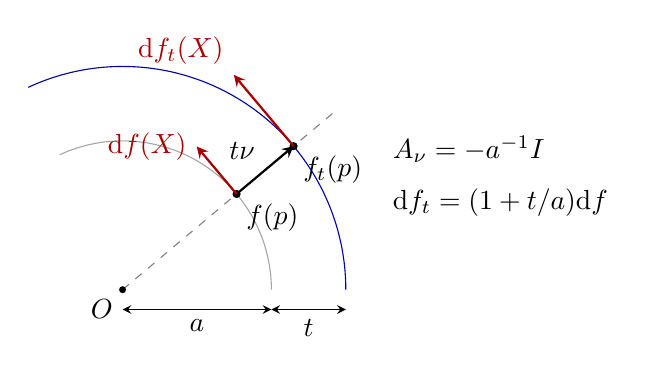
\begin{tikzpicture}[scale=1.05,>=stealth]
	\draw[gray!70] (0:1.8) arc[start angle=0,end angle=115,radius=1.8];
	\draw[blue!65!black] (0:2.7) arc[start angle=0,end angle=115,radius=2.7];
	\draw[gray,dashed] (0,0)--(40:3.35);
	\coordinate (P) at (40:1.8);
	\coordinate (Q) at (40:2.7);
	\fill (0,0) circle (1.2pt) node[below left]{\(O\)};
	\fill (P) circle (1.4pt) node[below right]{\(f(p)\)};
	\fill (Q) circle (1.4pt) node[below right]{\(f_t(p)\)};
	\draw[->,thick] (P)--(Q) node[midway,above left]{\(t\nu\)};
	\draw[->,thick,red!65!black] (P)--++(130:0.75) node[left]{\(\mathrm df(X)\)};
	\draw[->,thick,red!65!black] (Q)--++(130:1.125) node[above left]{\(\mathrm df_t(X)\)};
	\draw[<->] (0,-0.24)--(1.8,-0.24) node[midway,below]{\(a\)};
	\draw[<->] (1.8,-0.24)--(2.7,-0.24) node[midway,below]{\(t\)};
	\node[anchor=west] at (3.15,1.7){\(A_\nu=-a^{-1}I\)};
	\node[anchor=west] at (3.15,1.05){\(\mathrm df_t=(1+t/a)\mathrm df\)};
\end{tikzpicture}

	\caption[圆周的法向偏移]{圆周的外法向偏移。相同角参数的切向微分从内圆移到外圆后放大为原来的 \(1+t/a\) 倍。}
	\label{g3:fig:normal-offset}
\end{figure}

\subsection{超曲面的主曲率}
\label{g3:subsec:0404:02}

余维一时，每个法向值都由一个实数确定。选定单位法向 \(\nu\) 后，写 \(B(X,Y)=g(AX,Y)\nu\)。自伴算子 \(A\) 在每一点有正交单位特征基，其特征值 \(\kappa_1,\ldots,\kappa_n\) 称为该法向下的\term[zhuqulv]{主曲率}[principal curvatures]，相应特征方向称为\term[zhufangxiang]{主方向}[principal directions]。重特征值处未必能把单个主方向光滑选出，下面的逐点公式不需要这种选择。

\begin{proposition}\label{g3:prop:principal-curvature-contractions}
	设 \(f:(M^n,g)\to\bar M^{n+1}\) 是光滑等距浸入，\(n\ge2\)，环境截面曲率恒为 \(c\)。在一点选单位法向 \(\nu\) 及主方向正交单位基 \((e_i)\)，令 \(H_\nu=\langle H,\nu\rangle=n^{-1}\sum_i\kappa_i\)。则
	\begin{align}
		K(e_i,e_j)&=c+\kappa_i\kappa_j\quad(i\ne j),\label{g3:eq:principal-sectional-curvature}\\
		\operatorname{Ric}(e_i,e_j)
		&=\bigl((n-1)c+nH_\nu\kappa_i-\kappa_i^2\bigr)\delta_{ij},\label{g3:eq:principal-ricci-curvature}\\
		\operatorname{Scal}
		&=n(n-1)c+n^2H_\nu^2-|A|^2.\label{g3:eq:hypersurface-scalar-curvature}
	\end{align}
\end{proposition}
\begin{proof}
	Gauss 方程在这组基中成为
	\[
		R_{ijkl}
		=c(\delta_{ik}\delta_{jl}-\delta_{il}\delta_{jk})
		+\kappa_i\kappa_j(\delta_{ik}\delta_{jl}-\delta_{il}\delta_{jk}).
	\]
	取 \(k=i,l=j\) 得到截面公式。固定 \(i\)，把它对 \(j\ne i\) 相加，得到
	\[
		\operatorname{Ric}(e_i,e_i)
		=(n-1)c+\kappa_i\Bigl(\sum_j\kappa_j-\kappa_i\Bigr).
	\]
	非对角分量由同一四阶公式为零。再对 \(i\) 求和，使用 \(|A|^2=\sum_i\kappa_i^2\)，即得标量曲率式。
\end{proof}

这些公式也给出外在形状的限制。例如 Euclid 超曲面若在一点平坦，则 \(\kappa_i\kappa_j=0\) 对所有 \(i\ne j\) 成立，故该点形算子的秩至多为一。若每个截面曲率都严格为正，则任意两个主曲率的乘积均为正，所有主曲率同号。另一方面，全脐点的 \(A=H_\nu I\) 使所有截面曲率等于 \(c+H_\nu^2\)。

\ProseParagraphBreak

法向偏移的主曲率可由式\eqref{g3:eq:parallel-hypersurface-shape}逐个读取：
\[
	\kappa_i(t)=\frac{\kappa_i}{1-t\kappa_i}.
\]
当某个 \(1-t\kappa_i\) 为零时，相应切向方向被 \(\mathrm df_t\) 压为零，偏移参数化失去浸入性。这是一个局部微分条件。即使这些因子都非零，不同基点的法线仍可能在远处相交，因此共同管状半径还需要控制整体单射性。

\subsection{内在曲率相同而外在几何不同}
\label{g3:subsec:0404:03}

内在度量记录沿子流形测量的长度，第二基本形式则记录切空间在环境中的转动。同一度量可以对应不同的第二基本形式；局部基本定理的唯一性因而需要完整的相容数据。

\begin{example}\label{g3:exm:plane-cylinder-isometry}
	在一个平面开矩形 \(U\subset\mathbb R^2\) 上，考虑
	\[
		f_0(u,v)=(u,v,0),\qquad
		f_a(u,v)=\bigl(a\cos(u/a),a\sin(u/a),v\bigr),\quad a>0.
	\]
	两者的诱导度量都是 \(\mathrm du^2+\mathrm dv^2\)，所以具有相同的内在距离局部结构和零 Gauss 曲率。对圆柱取外法向
	\[
		\nu(u,v)=\bigl(\cos(u/a),\sin(u/a),0\bigr),
	\]
	则 \(A_\nu\partial_u=-a^{-1}\partial_u\)、\(A_\nu\partial_v=0\)，而平面上 \(B=0\)。故两者不可能在任何开集上由一个 Euclid 刚性运动联系：环境等距保持第二基本形式，尤其保持其范数。这里一个范数为零，另一个为 \(a^{-1}\)。

	若允许 \(u\) 遍历整个实轴，\(f_a(u+2\pi a,v)=f_a(u,v)\)。因此这个局部等距参数化在整个平面上不单射；把参数域限制到适当的小矩形后，才得到到一块圆柱面的等距微分同胚。
\end{example}

上述区别在高余维中还包括法联络。即使给定相同的 \(g\) 和对称型的分量，换法标架时也必须同时按同一个丛等距变换法联络与 \(B\)。三组相容方程正是对这套几何数据的条件；只比较一张矩阵或只比较内在曲率，不能使用基本定理的唯一性结论。

\subsection{面积变分与平均曲率}
\label{g3:subsec:0404:04}

当浸入随参数移动时，切向速度主要改变参数点的分布，法向速度才直接与平均曲率配对。先计算诱导度量及其体积密度的导数，便能在任意维数、任意余维得到面积的一阶公式。这里“面积”指 \(n\) 维诱导体积；对非单射浸入按参数流形积分，保留重数。

\begin{theorem}[面积的一阶变分]\label{g3:thm:first-variation-submanifold-area}
	设 \(F:(-\varepsilon,\varepsilon)\times M^n\to(\bar M,\bar g)\) 光滑，每个 \(f_t=F(t,\cdot)\) 都是浸入，\(n\ge1\)。记 \(g_t=f_t^*\bar g\)、\(g=g_0\)，并将初速度分解为 \(V=\partial_tF|_0=\mathrm df_0(W)+V^\perp\)。则
	\begin{align}
		\dot g_0(X,Y)
		&=g(\nabla_XW,Y)+g(X,\nabla_YW)
		-2\langle B(X,Y),V^\perp\rangle,\label{g3:eq:variation-induced-metric}\\
		\left.\frac{\mathrm d}{\mathrm dt}\right|_0\mu_{g_t}
		&=\bigl(\operatorname{div}_gW-n\langle H,V^\perp\rangle\bigr)\mu_g.\label{g3:eq:variation-induced-density}
	\end{align}
	若 \(\Omega\subset M\) 是具有光滑边界的紧区域，\(\eta\) 是 \(\partial\Omega\) 在 \(M\) 内的外单位法向，则
	\begin{equation}\label{g3:eq:first-variation-area-integral}
		\left.\frac{\mathrm d}{\mathrm dt}\right|_0\operatorname{Vol}_{g_t}(\Omega)
		=\int_{\partial\Omega}g(W,\eta)\mu_{\partial g}
		-n\int_\Omega\langle H,V^\perp\rangle\mu_g.
	\end{equation}
\end{theorem}
\begin{proof}
	把 \(X,Y\) 延拓成与时间无关的参数向量场。环境联络度量相容且无挠，因而沿二参数坐标面有 \(\bar\nabla_t\mathrm df_t(X)=\bar\nabla_X\partial_tF\)。逐项求导得到
	\[
		\dot g_0(X,Y)
		=\langle\bar\nabla_XV,\mathrm df_0(Y)\rangle
		+\langle\mathrm df_0(X),\bar\nabla_YV\rangle.
	\]
	代入 \(V=\mathrm df_0(W)+V^\perp\)，用 Gauss 分解和 Weingarten 公式提取切向分量，便得度量变化式。

	在任一固定坐标中，密度系数为 \(\sqrt{\det g_t}\)。可逆矩阵的行列式求导给出
	\[
		\left.\frac{\mathrm d}{\mathrm dt}\right|_0\sqrt{\det g_t}
		=\frac12\operatorname{tr}_g(\dot g_0)\sqrt{\det g}.
	\]
	在一点取正交单位基求迹，前两项各贡献 \(\operatorname{div}_gW\)，最后一项贡献 \(-2n\langle H,V^\perp\rangle\)。这证明密度公式。紧区域上可在积分号下求导，再对 \(W\) 使用\cref{g3:thm:divergence-theorem}，得到边界通量。密度与该散度定理均不要求 \(M\) 可定向。
\end{proof}

\begin{corollary}\label{g3:cor:minimal-area-stationarity}
	设 \(f:M^n\to\bar M\) 为光滑浸入，\(n\ge1\)，\(M\) 无边界。则 \(H=0\) 当且仅当对于任意具有光滑边界的紧区域 \(\Omega\subset M\)，以及任意满足 \(\operatorname{supp}V\subset\operatorname{int}\Omega\) 的上述光滑变分，都有 \(\left.\frac{\mathrm d}{\mathrm dt}\right|_0\operatorname{Vol}_{g_t}(\Omega)=0\)。
\end{corollary}
\begin{proof}
	若 \(H=0\)，在包含初速度支集的紧区域上应用式\eqref{g3:eq:first-variation-area-integral}，边界项和内部项都为零。反过来，若某点 \(H\ne0\)，在其附近选一个非负光滑截断函数 \(\chi\)，支集紧含于一个坐标片，且在该点附近为正。取法向初速度 \(V=\chi H\)。它可以由变分
	\[
		f_t(p)=\exp^{\bar g}_{f(p)}(tV(p))
	\]
	实现：支集紧使共同的小时间可用，指数映射的联合光滑性见\cref{g3:prop:exponential-local}；浸入性是开条件，在这个紧支集上缩小时间便仍成立，支集外则保持原映射。此时一阶变分为 \(-n\int\chi|H|^2\mu_g<0\)，与驻定性矛盾。因此 \(H\) 必处处为零。
\end{proof}

这一结论说明“极小”的一阶意义是面积驻定。是否在所有邻近变分下取得局部最小值，还需要二阶变化的信息。球面外移的检验则直接固定本章符号：若 \(V=\nu\)、\(H=-\nu/a\)，密度导数为 \(n\mu_g/a>0\)，与半径增大一致。

\begin{proposition}\label{g3:prop:immersion-position-laplacian}
	设 \(f:(M^n,g)\to\mathbb R^{n+r}\) 为光滑等距浸入，\(n\ge1\)，对位置向量的各坐标分别使用 \(\Delta_g=-\operatorname{div}_g\operatorname{grad}_g\)。则
	\begin{equation}\label{g3:eq:position-laplacian}
		\Delta_g f=-nH,\qquad
		\Delta_g|f|^2=-2n-2n\langle f,H\rangle.
	\end{equation}
	若像位于 \(S^{n+r-1}(a)\)，以 \(H^S\) 表示相对于球面的平均曲率向量，则
	\begin{equation}\label{g3:eq:spherical-minimal-eigenmap}
		H^{\mathbb R}=H^S-\frac f{a^2},\qquad
		H^S=0\ \Longleftrightarrow\ \Delta_g f=\frac n{a^2}f.
	\end{equation}
\end{proposition}
\begin{proof}
	对任一坐标函数 \(f^\alpha\)，Hessian 的定义给出
	\[
		H_{f^\alpha}(X,Y)
		=\bigl(\mathrm D_X\mathrm df(Y)-\mathrm df(\nabla_XY)\bigr)^\alpha
		=B(X,Y)^\alpha.
	\]
	取负迹即得 \(\Delta_g f=-nH\)。由乘积法则，
	\[
		\Delta_g|f|^2=2\langle f,\Delta_g f\rangle-2|\mathrm df|^2.
	\]
	等距浸入使 \(|\mathrm df|^2=n\)，故得第二式。若像在半径 \(a\) 的球面内，先将环境导数投影到球面的切空间，再投影到 \(M\) 的切空间；球面自身的第二基本形式为 \(-g f/a^2\)。于是
	\[
		B^{\mathbb R}(X,Y)=B^S(X,Y)-\frac{g(X,Y)}{a^2}f.
	\]
	取平均迹得到两个平均曲率的关系，再代入位置向量的 Laplace 公式，便得最后的等价式。
\end{proof}

\begin{corollary}\label{g3:cor:no-compact-euclidean-minimal}
	正维紧无边界光滑流形不存在到 Euclid 空间的极小浸入。
\end{corollary}
\begin{proof}
	若有这样的浸入，以诱导度量计算，由 \(H=0\) 及式\eqref{g3:eq:position-laplacian}，有 \(\Delta_g|f|^2=-2n\)。在 \(M\) 上积分，散度定理使左边为零，右边却是 \(-2n\operatorname{Vol}_g(M)<0\)，矛盾。
\end{proof}

球面中的极小乘积没有这一矛盾：其 Euclid 平均曲率为 \(-f/a^2\)，在位置向量公式中恰好抵消常数项。这样，局部的切法分解、相容方程及整体积分在同一个模型上相互核对。


\begin{chaptersummary}
	切向与法向投影把环境导数分成内在 Levi-Civita 联络、第二基本形式、形算子及法联络。第二基本形式的对称性来自无挠性，形算子是它与指定法向配对后的自伴算子，平均曲率向量则是其平均迹。高余维法空间的变化具有自己的曲率，不能由单个形算子代替。

	\ProseParagraphBreak

	Gauss、Codazzi 和 Ricci 方程分别比较切曲率、第二基本形式的导数与法曲率。在空间形式中，它们恰好使所构造的切法直和联络或其增广联络平坦。积分平坦标架，再积分位置数据，就得到局部浸入；同一数据的两次构造相差环境等距。整体实现还要求沿闭路的标架返回以及 Euclid 情形的位置周期相容，局部方程本身不会消去这些障碍。

	\ProseParagraphBreak

	模型计算展示了内在和外在信息的不同作用：平面与圆柱可以局部等距，球面乘积可以在球面内极小而在 Euclid 空间中不极小，法向偏移的正则性则由形算子的特征值控制。面积的一阶变化由边界通量与平均曲率配对给出；无边界紧支变分下，\(H=0\) 等价于面积驻定。位置向量的 Laplace 公式进一步把这一外在条件转化为可积分的函数等式。
\end{chaptersummary}

\BookExercises

\begin{exercise}\label{g3:ex:graph-prescribed-second-fundamental-form}
	设 \(h:U\to\mathbb R^r\) 光滑，其中 \(U\subset\mathbb R^n\) 为原点邻域，\(n\ge1\)，且 \(h(0)=0\)、\(\mathrm dh_0=0\)。考虑图像浸入
	\[
		f(x)=(x,h(x))\in\mathbb R^{n+r},
	\]
	并给 \(U\) 诱导度量。
	\begin{enumerate}
		\item 求原点处的度量、联络系数、第二基本形式及平均曲率向量。将形算子写成 \(h\) 的二阶偏导矩阵。
		\item 给定任意对称双线性映射 \(C:\mathbb R^n\times\mathbb R^n\to\mathbb R^r\)，构造一个这样的图像，使其原点第二基本形式等于 \(C\)。当 \(n\ge2\)、\(r\ge1\) 时，给出 \(H(0)=0\) 而 \(B_0\ne0\) 的具体例子。
	\end{enumerate}
\end{exercise}
\begin{solution}
	1. 记 \(h_i^\alpha=\partial_i h^\alpha\)。坐标切向量及度量为
	\[
		f_i=(e_i,h_i),\qquad
		g_{ij}=\delta_{ij}+\sum_{\alpha=1}^r h_i^\alpha h_j^\alpha.
	\]
	因为 \(h_i^\alpha(0)=0\)，有 \(g_{ij}(0)=\delta_{ij}\)，且
	\[
		\partial_kg_{ij}(0)
		=\sum_\alpha
			\bigl(h_{ik}^\alpha h_j^\alpha+h_i^\alpha h_{jk}^\alpha\bigr)(0)=0.
	\]
	由 Christoffel 公式，\(\Gamma^k_{ij}(0)=0\)。原点切空间是水平的 \(\mathbb R^n\times\{0\}\)，法空间是竖直的 \(\{0\}\times\mathbb R^r\)，而
	\[
		\partial_i\partial_jf(0)
		=\left(0,\bigl(\partial_i\partial_jh^\alpha(0)\bigr)_{\alpha=1}^r\right)
	\]
	已经法向。因此
	\[
		B_0(e_i,e_j)
		=\left(0,\bigl(\partial_i\partial_jh^\alpha(0)\bigr)_\alpha\right),
		\qquad
		H(0)=\frac1n
			\left(0,\bigl(\sum_i\partial_i^2h^\alpha(0)\bigr)_\alpha\right).
	\]
	对法向量 \(\xi=(0,\xi^1,\ldots,\xi^r)\)，形算子在水平正交基中的矩阵为
	\[
		(A_\xi)_{ij}
		=\sum_{\alpha=1}^r\xi^\alpha\partial_i\partial_jh^\alpha(0).
	\]
	矩阵对称，对应 \(B\) 的对称性。这里原点处 \(\partial g=0\) 已足以计算联络与 \(B\)，不需要把整个图像坐标识别为法坐标。

	2. 写 \(C(e_i,e_j)=C_{ij}\in\mathbb R^r\)，并取
	\[
		h(x)=\frac12C(x,x)=\frac12\sum_{i,j}C_{ij}x^ix^j.
	\]
	对称性给出 \(\partial_i\partial_jh=C_{ij}\)，且 \(h(0)=0\)、\(\mathrm dh_0=0\)。图像的前 \(n\) 个分量就是 \(x\)，所以处处为浸入；第 1 问表明其原点第二基本形式恰为给定的 \(C\)。

	当 \(n\ge2\)、\(r\ge1\) 时，取
	\[
		h^1(x)=\frac12\bigl((x^1)^2-(x^2)^2\bigr),\qquad
		h^\alpha(x)=0\quad(\alpha>1).
	\]
	记 \(\varepsilon_1\) 为 \(\mathbb R^r\) 的第一个标准基向量。原点处 \(B(e_1,e_1)=(0,\varepsilon_1)\)、\(B(e_2,e_2)=-(0,\varepsilon_1)\)，其他对角分量为零，因此 \(H(0)=0\)，但 \(B_0\ne0\)。这显示一点处平均曲率为零允许不同切向方向的法向弯曲相互抵消。
\end{solution}

\begin{exercise}\label{g3:ex:normal-frame-change}
	设 \(f:(M,g)\to(\bar M,\bar g)\) 为光滑等距浸入，在开集 \(U\subset M\) 上取正交单位法标架 \(\nu=(\nu_1,\ldots,\nu_r)\)，写
	\(\nabla^\perp\nu=\nu\eta\)、\(F^\perp=\mathrm d\eta+\eta\wedge\eta\)。
	\begin{enumerate}
		\item 若 \(\nu'=\nu Q\)，其中 \(Q:U\to\operatorname{O}(r)\) 光滑，证明
		\[
			\eta'=Q^{-1}\eta Q+Q^{-1}\mathrm dQ,\qquad
			(F^\perp)'=Q^{-1}F^\perp Q.
		\]
		\item 设法丛秩为二，在定向正交单位法标架中写
		\[
			\eta=\begin{pmatrix}0&-\alpha\\\alpha&0\end{pmatrix}.
		\]
		若 \(Q\) 为角度 \(\phi\) 的转动矩阵，求 \(\alpha'\)。进一步，若 \(U\) 是二维坐标矩形，证明在 \(U\) 上存在由这种转动得到的法平行标架，当且仅当 \(\mathrm d\alpha=0\)。充分性中直接构造 \(\phi\)。
	\end{enumerate}
\end{exercise}
\begin{solution}
	1. 联络的乘积规则给出
	\[
		\nabla^\perp(\nu Q)=\nu(\eta Q+\mathrm dQ)
		=\nu Q\bigl(Q^{-1}\eta Q+Q^{-1}\mathrm dQ\bigr),
	\]
	所以括号中就是新标架的联络矩阵。曲率对法向输入为函数线性，故
	\[
		R^\perp(X,Y)(\nu Q)=\nu F^\perp(X,Y)Q
		=\nu Q\bigl(Q^{-1}F^\perp(X,Y)Q\bigr).
	\]
	这证明曲率矩阵按共轭变换，并由此再见 \(R^\perp\) 是否为零与标架无关。

	2. 记
	\[
		J=\begin{pmatrix}0&-1\\1&0\end{pmatrix},\qquad
		Q=\begin{pmatrix}\cos\phi&-\sin\phi\\
			\sin\phi&\cos\phi\end{pmatrix}.
	\]
	\(JQ=QJ\)，且 \(Q^{-1}\mathrm dQ=J\,\mathrm d\phi\)，所以
	\[
		\eta'=J(\alpha+\mathrm d\phi),\qquad
		\alpha'=\alpha+\mathrm d\phi.
	\]
	又因 \(\alpha\wedge\alpha=0\)，有 \(F^\perp=J\,\mathrm d\alpha\)。若转动后标架法平行，则 \(\alpha'=0\)，从而 \(\mathrm d\alpha=0\)。

	反过来，在坐标矩形上写 \(\alpha=a(x,y)\,\mathrm dx+b(x,y)\,\mathrm dy\)，并固定其中一点 \((x_0,y_0)\)。闭性意味着 \(\partial_xb=\partial_ya\)。令
	\[
		\phi(x,y)
		=-\int_{x_0}^x a(t,y_0)\,\mathrm dt
			-\int_{y_0}^y b(x,s)\,\mathrm ds.
	\]
	矩形保证两段积分道路都在坐标域内。直接求导，
	\[
		\partial_y\phi=-b(x,y),\qquad
		\partial_x\phi=-a(x,y_0)
			-\int_{y_0}^y\partial_xb(x,s)\,\mathrm ds=-a(x,y).
	\]
	故 \(\mathrm d\phi=-\alpha\)，从而 \(\alpha'=0\)，所得正交单位法标架处处法平行。矩形条件在这里提供了单值的原函数构造；只有一点处曲率为零，并不足以使这一构造适用于整个邻域。
\end{solution}

\begin{exercise}\label{g3:ex:helix-normal-parallel-frame}
	设 \(a>0\)、\(b\ne0\)、\(c=\sqrt{a^2+b^2}\)，考虑 Euclid 空间中的单位速曲线
	\[
		\gamma(s)=\left(a\cos\frac sc,\ a\sin\frac sc,\ \frac bc s\right),
		\qquad s\in\mathbb R.
	\]
	记 \(T=\gamma'\)，并定义
	\[
		\nu_1(s)=\left(-\cos\frac sc,-\sin\frac sc,0\right),\qquad
		\nu_2(s)=\left(\frac bc\sin\frac sc,-\frac bc\cos\frac sc,\frac ac\right).
	\]
	\begin{enumerate}
		\item 验证 \((T,\nu_1,\nu_2)\) 为正交单位标架，求第二基本形式、平均曲率向量及法联络矩阵。
		\item 构造整个参数直线上的正交单位法平行标架。说明法平行不等于作为 \(\mathbb R^3\) 中的向量保持不变。
		\item 证明此曲线的法联络曲率为零，但其平均曲率向量不法平行，虽然 \(|H|\) 为常数。
	\end{enumerate}
\end{exercise}
\begin{solution}
	1. 求导得到
	\[
		T=\left(-\frac ac\sin\frac sc,\frac ac\cos\frac sc,\frac bc\right).
	\]
	由 \(a^2+b^2=c^2\)，三个向量的长度都为一，互相内积为零。令
	\[
		\kappa=\frac a{c^2},\qquad \tau=\frac b{c^2}.
	\]
	直接求导并在此标架中分解，得到
	\[
		T'=\kappa\nu_1,\qquad
		\nu_1'=-\kappa T+\tau\nu_2,\qquad
		\nu_2'=-\tau\nu_1.
	\]
	参数直线取诱导度量 \(\mathrm ds^2\)。于是
	\[
		B(\partial_s,\partial_s)=H=\kappa\nu_1,\qquad
		\nabla^\perp_{\partial_s}\nu_1=\tau\nu_2,\qquad
		\nabla^\perp_{\partial_s}\nu_2=-\tau\nu_1.
	\]
	行标架 \(\nu=(\nu_1,\nu_2)\) 的法联络矩阵为
	\[
		\eta=\begin{pmatrix}0&-\tau\\\tau&0\end{pmatrix}\mathrm ds.
	\]

	2. 取转动角 \(\phi(s)=-\tau s\)，并令
	\[
		\begin{aligned}
			E_1&=\cos(\tau s)\nu_1-\sin(\tau s)\nu_2,\\
			E_2&=\sin(\tau s)\nu_1+\cos(\tau s)\nu_2.
		\end{aligned}
	\]
	这是处处正交的转动，所以 \((E_1,E_2)\) 仍为正交单位法标架。利用第 1 问的导数式，各个法向项逐对抵消，得到
	\[
		E_1'=-\kappa\cos(\tau s)T,\qquad
		E_2'=-\kappa\sin(\tau s)T.
	\]
	两个导数都切向，故 \(\nabla^\perp_{\partial_s}E_1=
	\nabla^\perp_{\partial_s}E_2=0\)。但 \(E_1'(0)=-\kappa T(0)\ne0\)，所以法平行向量场仍可以作为环境向量改变；改变的部分恰好全部切向。

	3. 法曲率对两个切向输入反对称，一维切空间中任意两个输入线性相关，故 \(R^\perp=0\)。在给定标架中也可直接计算：\(\mathrm d\eta=0\)，且 \(\eta\wedge\eta\) 含因子 \(\mathrm ds\wedge\mathrm ds=0\)。另一方面，
	\[
		|H|=\kappa,\qquad
		\nabla^\perp_{\partial_s}H
		=\kappa\tau\nu_2\ne0,
	\]
	因为 \(\kappa>0\)、\(\tau\ne0\)。法联络平坦、某个法向场长度恒定、该法向场法平行，是三个不同的条件。
\end{solution}

% 第三卷第四章习题草稿：一般余维收缩、极小浸入、二维法曲率。
% 合入章文件后由章内环境连续编号。

\begin{exercise}\label{g3:ex:submanifold-ricci-scalar-contractions}
	设 \(F\colon(M^n,g)\to\bar M^{n+q}\) 为到常截面曲率 \(c\) 空间的光滑等距浸入，\(n\ge2\)。令 \(B\) 为第二基本形式，\(H=\operatorname{tr}_gB/n\)，并对任一正交单位基 \((e_i)\) 定义
	\[
		\lVert B\rVert^2=\sum_{i,j}\lVert B(e_i,e_j)\rVert^2,
		\qquad B^\circ(X,Y)=B(X,Y)-g(X,Y)H.
	\]
	由 Gauss 方程求 \(\operatorname{Ric}\) 与 \(\operatorname{Scal}\) 的一般余维表达式，证明
	\[
		\operatorname{Scal}\le n(n-1)(c+\lVert H\rVert^2),
	\]
	并用 \(B^\circ\) 描述逐点取等的充要条件。最后说明最小维数 \(n=2\) 时所得不等式的几何含义。
\end{exercise}
\begin{solution}
	固定一点，并在该点取正交单位基 \((e_i)\)。按照本卷的曲率次序，\(\operatorname{Ric}(X,Y)=\sum_i\mathrm{Rm}(e_i,X,e_i,Y)\)。对 \eqref{g3:eq:gauss-space-form} 收缩，环境项为
	\[
		c\sum_i\bigl(g(X,Y)-g(e_i,Y)g(X,e_i)\bigr)
		=(n-1)c\,g(X,Y).
	\]
	第二基本形式的两个项分别给出
	\[
		\sum_i\langle B(e_i,e_i),B(X,Y)\rangle
		=n\langle H,B(X,Y)\rangle,
	\]
	以及 \(-\sum_i\langle B(X,e_i),B(Y,e_i)\rangle\)。因此
	\[
		\operatorname{Ric}(X,Y)
		=(n-1)c\,g(X,Y)+n\langle H,B(X,Y)\rangle
		-\sum_i\langle B(X,e_i),B(Y,e_i)\rangle.
	\]
	再取迹得到
	\[
		\operatorname{Scal}
		=n(n-1)c+n^2\lVert H\rVert^2-\lVert B\rVert^2.
	\]
	以上均为张量的度量收缩，所以不依赖所取正交单位基。

	展开无迹部分的平方，利用 \(\sum_iB(e_i,e_i)=nH\)，有
	\[
		\begin{aligned}
		\lVert B^\circ\rVert^2
		&=\sum_{i,j}\lVert B(e_i,e_j)-\delta_{ij}H\rVert^2\\
		&=\lVert B\rVert^2-2\sum_i\langle B(e_i,e_i),H\rangle
		+n\lVert H\rVert^2\\
		&=\lVert B\rVert^2-n\lVert H\rVert^2.
		\end{aligned}
	\]
	于是精确的差值是
	\[
		\operatorname{Scal}
		=n(n-1)(c+\lVert H\rVert^2)-\lVert B^\circ\rVert^2.
	\]
	范数平方非负给出题设不等式，且某点取等当且仅当 \(B^\circ=0\)，即该点满足 \(B(X,Y)=g(X,Y)H\)，正是脐点条件。当 \(n=2\) 时，\(\operatorname{Scal}=2K\)，所以
	\[
		K=c+\lVert H\rVert^2-\tfrac12\lVert B^\circ\rVert^2
		\le c+\lVert H\rVert^2.
	\]
	因此在环境曲率和平均曲率向量给定时，偏离脐性的部分精确降低了内在 Gauss 曲率。
\end{solution}

\begin{exercise}\label{g3:ex:minimal-euclidean-ricci-nullity}
	设 \(F\colon(M^n,g)\to\mathbb R^{n+q}\) 为光滑极小等距浸入，即 \(H=0\)。证明 \(\operatorname{Ric}\) 为半负定，并求出其作为双线性型的核
	\[
		\ker\operatorname{Ric}_p
		=\{v\in\mathrm{T}_pM:\operatorname{Ric}_p(v,w)=0
		\text{ 对每个 }w\in\mathrm{T}_pM\}.
	\]
	进一步证明 \(\operatorname{Ric}_p=0\) 当且仅当 \(B_p=0\)，并推出：若一个极小 Euclid 浸入的诱导度量平直，则它全测地。解释为何删除极小性后最后一个结论不再成立。
\end{exercise}
\begin{solution}
	由上一题的 Ricci 收缩公式，令 \(c=0\)、\(H=0\)，便有
	\[
		\operatorname{Ric}_p(v,w)
		=-\sum_i\langle B_p(v,e_i),B_p(w,e_i)\rangle.
	\]
	特别地，\(\operatorname{Ric}_p(v,v)=-\sum_i\lVert B_p(v,e_i)\rVert^2\le0\)。如果 \(v\) 属于 Ricci 型的核，取 \(w=v\) 可知每个 \(B_p(v,e_i)\) 都为零，故由线性性 \(B_p(v,w)=0\) 对任意 \(w\) 成立。反过来，若这一条件成立，所显示的双线性公式立即给出 \(v\in\ker\operatorname{Ric}_p\)。因此
	\[
		\ker\operatorname{Ric}_p
		=\{v\in\mathrm{T}_pM:B_p(v,w)=0\text{ 对所有 }w\in\mathrm{T}_pM\}.
	\]
	若 \(\operatorname{Ric}_p=0\)，上述核就是整个切空间，所以 \(B_p=0\)；反向蕴含也由同一公式得到。

	若诱导度量平直，则每点的 Ricci 张量为零，因而 \(B=0\)。由 \cref{g3:prop:totally-geodesic-characterization}，浸入全测地。这里用到了极小性：例如半径为 \(a>0\) 的圆柱
	\[
		F(s,t)=(a\cos(s/a),a\sin(s/a),t)
	\]
	诱导度量为 \(\mathrm ds^2+\mathrm dt^2\)，但采用外法向时，\(B(\partial_s,\partial_s)=-\nu/a\)、\(B(\partial_t,\partial_t)=B(\partial_s,\partial_t)=0\)，所以 \(B\ne0\) 且 \(H=-\nu/(2a)\ne0\)。平直性本身不排除这种弯曲。
\end{solution}

\begin{exercise}\label{g3:ex:minimal-surface-normal-curvature-bound}
	设 \(F\colon M^2\to\mathbb R^4\) 为光滑极小等距浸入，在一点 \(p\) 选取切空间和法空间的正交单位基 \((e_1,e_2)\)、\((\nu_1,\nu_2)\)。由于极小性，可写
	\[
		A_{\nu_1}=\begin{pmatrix}a&b\\b&-a\end{pmatrix},
		\qquad
		A_{\nu_2}=\begin{pmatrix}c&d\\d&-c\end{pmatrix}.
	\]
	记 \(K\) 为内在 Gauss 曲率，并相对于所选两组基定义
	\[
		K^\perp=\langle R^\perp(e_1,e_2)\nu_1,\nu_2\rangle.
	\]
	计算 \(K\) 与 \(K^\perp\)，证明 \(\lvert K^\perp\rvert\le-K\)，并给出取等条件。将等号条件解释为法平面内曲线
	\[
		\theta\longmapsto
		B(\cos\theta\,e_1+\sin\theta\,e_2,
		  \cos\theta\,e_1+\sin\theta\,e_2)
	\]
	的几何性质，允许该曲线退化为一点。
\end{exercise}
\begin{solution}
	把法平面用所选基识别为 \(\mathbb R^2\)，则
	\[
		u\coloneqq B(e_1,e_1)=(a,c),\qquad
		v\coloneqq B(e_1,e_2)=(b,d),\qquad
		B(e_2,e_2)=-u.
	\]
	Gauss 方程给出
	\[
		K=-\lVert u\rVert^2-\lVert v\rVert^2
		=-(a^2+b^2+c^2+d^2).
	\]
	Ricci 方程则给出 \(K^\perp=g([A_{\nu_1},A_{\nu_2}]e_1,e_2)\)。直接相乘有
	\[
		[A_{\nu_1},A_{\nu_2}]
		=\begin{pmatrix}0&2(ad-bc)\\2(bc-ad)&0\end{pmatrix},
	\]
	所以在本卷的符号约定下，
	\[
		K^\perp=2(bc-ad)=-2\det(u,v).
	\]
	反转任一组基的定向会改变 \(K^\perp\) 的符号，但不影响下面的绝对值不等式。利用平面行列式的估计和平方差，有
	\[
		\lvert K^\perp\rvert
		=2\lvert\det(u,v)\rvert
		\le2\lVert u\rVert\lVert v\rVert
		\le\lVert u\rVert^2+\lVert v\rVert^2=-K.
	\]
	两步同时取等当且仅当 \(u\perp v\) 且 \(\lVert u\rVert=\lVert v\rVert\)，其中包括 \(u=v=0\)。用矩阵分量写为
	\[
		ab+cd=0,\qquad a^2+c^2=b^2+d^2.
	\]
	最后利用双线性和 \(B(e_2,e_2)=-u\)，题设曲线为
	\[
		u\cos(2\theta)+v\sin(2\theta).
	\]
	它是单位圆在以 \(u,v\) 为列向量的线性映射下的像，通常为椭圆。若 \(u,v\) 正交且等长，则其像为以原点为圆心的圆；两者都为零时退化为原点。反过来，若此像是半径 \(\rho>0\) 的圆，则在 \(2\theta=0,\pi/2,\pi/4\) 处比较到原点的距离，先得 \(\lVert u\rVert=\lVert v\rVert=\rho\)，再得 \(\langle u,v\rangle=0\)。退化为一点时，其中心为原点且 \(u=v=0\)。故题设不等式取等恰好对应这一个圆形或点形的情形。
\end{solution}

\begin{exercise}\label{g3:ex:normal-data-gauge-equivalence}
	设 \((M,g)\) 为无边界光滑黎曼流形，\(E,E'\to M\) 为同秩光滑 Euclid 向量丛，\(J:E\to E'\) 是覆盖恒等映射的光滑纤维等距。给定 \(E\) 上的度量联络 \(\nabla^E\) 与光滑对称型 \(B\in\Gamma(\operatorname{Sym}^2\mathrm T^*M\otimes E)\)，在 \(E'\) 上定义
	\[
		B'(X,Y)=J B(X,Y),\qquad
		\nabla^{E'}_X\xi'=J\bigl(\nabla^E_X(J^{-1}\xi')\bigr).
	\]
	\begin{enumerate}
		\item 证明新旧数据同时满足给定 \(c\) 的三组相容方程，并求两个数据联络之间的关系。
		\item 若 \((f,\iota)\) 实现原数据，写出实现新数据的同一个浸入的法丛识别。说明为什么旋转法标架时不能只旋转 \(B\) 的分量而保持联络矩阵不变。
	\end{enumerate}
\end{exercise}
\begin{solution}
	1. 由定义及 \(J\) 保持内积，\(\nabla^{E'}\) 满足联络的乘积规则并保持新内积。对 \(\xi\in\Gamma(E)\)，形算子满足
	\[
		g(A'_{J\xi}X,Y)
		=\langle JB(X,Y),J\xi\rangle_{E'}
		=g(A_\xi X,Y),
	\]
	所以 \(A'_{J\xi}=A_\xi\)。连续使用两次联络定义，得到
	\[
		R^{E'}(X,Y)(J\xi)=J(R^E(X,Y)\xi),
		\qquad(\nabla B')(X;Y,Z)=J((\nabla B)(X;Y,Z)).
	\]
	Gauss 式中的内积不变，Codazzi 的两边同乘 \(J\)，Ricci 式的两边也由上述曲率与形算子关系保持。因此相容性等价。

	令 \(L=\operatorname{id}_{\mathrm TM}\oplus J\)。对式\eqref{g3:eq:submanifold-data-connection}逐项代入，得到
	\[
		D'_X(L\sigma)=L(D_X\sigma).
	\]
	若 \(c\ne0\)，把 \(L\) 扩充为在 \(s\) 上取恒等，同样有 \(\widehat D'_XL=L\widehat D_X\)。所以两个数据联络只是经同一个纤维等距识别后的同一联络；平坦性及沿闭路径的返回条件同时成立。

	2. 取 \(\iota'=\iota\circ J^{-1}\)。则
	\[
		\iota'B'=\iota B=B_f,
		\qquad
		\nabla^{\perp,f}_X(\iota'\xi')
		=\iota'(\nabla^{E'}_X\xi'),
	\]
	故 \((f,\iota')\) 实现新数据。

	再用矩阵说明旋转标架的影响。设 \(\nu\) 是同一个法丛中的行正交标架，\(\nabla^E\nu=\nu\omega\)，并换为 \(\nu'=\nu O\)，其中 \(O:M\to\operatorname O(r)\) 光滑。由乘积规则，
	\[
		\omega'=O^{-1}\omega O+O^{-1}\mathrm dO.
	\]
	若 \(B=\nu b\)，其新分量为 \(b'=O^{-1}b\)。额外的 \(O^{-1}\mathrm dO\) 记录法标架自身的变化，必须与 \(B\) 分量的变化同时计入。例如在区间上，原联络矩阵为零，取
	\[
		O(s)=\begin{pmatrix}\cos s&-\sin s\\ \sin s&\cos s\end{pmatrix},
	\]
	则新矩阵为 \(\left(\begin{smallmatrix}0&-1\\1&0\end{smallmatrix}\right)\mathrm ds\)，并不为零。把它强行保持为零，会换掉法联络，因而改变给定的几何数据。
\end{solution}

\begin{exercise}\label{g3:ex:fundamental-theorem-smooth-families}
	设 \(U_0\subset\mathbb R^n\) 是含原点的开集，\(\lambda\) 属于 \(0\) 的有限维参数邻域。记 \(M=U_0\)，\(g_\lambda\) 为黎曼度量，\(\nabla^{E,\lambda}\) 为所给纤维内积的度量联络，\(B_\lambda\) 为光滑对称 \(E\) 值二阶型。固定 \(c\in\mathbb R\)，在 \(U_0\) 上给定一族数据 \((g_\lambda,E,\langle\ ,\ \rangle_\lambda,\nabla^{E,\lambda},B_\lambda)\)，其中 \(E=U_0\times\mathbb R^r\)，所有局部分量对 \((x,\lambda)\) 联合光滑，各纤维内积正定，每组数据都满足曲率 \(c\) 的相容方程。
	\begin{enumerate}
		\item 在原点给定光滑依赖 \(\lambda\) 的初始线性等距：\(c=0\) 时从 \((\mathrm TM\oplus E)_0\) 到 \(\mathbb R^{n+r}\)，\(c\ne0\) 时从增广纤维 \((\mathrm TM\oplus E\oplus\mathbb Rs)_0\) 到相应的线性环境空间。Euclid 情形再给定光滑的初始位置；\(c<0\) 时要求初始等距将 \(s_0\) 送到最后一坐标为正的单位向量。证明缩小坐标域与参数域后，可以选择实现 \((f_\lambda,\iota_\lambda)\) 对 \((x,\lambda)\) 联合光滑，并具有所给初值。
		\item 若 \(\lambda\) 为实参数，且 \(g_\lambda=g\) 不变，令 \(V=\left.\partial_\lambda f_\lambda\right|_{\lambda=0}\)。证明
		\[
			\langle\nabla^{Q}_X V,\mathrm df_0(Y)\rangle
			+\langle\mathrm df_0(X),\nabla^{Q}_Y V\rangle=0.
		\]
		将 \(V=\mathrm df_0(Z)+\eta\) 分成切向与法向后，把这一式子写成 \(Z,\eta,B_{f_0}\) 的关系。
	\end{enumerate}
\end{exercise}
\begin{solution}
	1. 因度量与纤维内积对参数光滑且在原点正定，可在共同小邻域中对固定基作逐次正交归一化；每一步只涉及光滑运算与正数开平方，故所得标架对 \((x,\lambda)\) 联合光滑。相应的 Levi-Civita 联络系数由度量、逆矩阵与一阶导数给出，故也联合光滑。于是式\eqref{g3:eq:submanifold-data-connection}或式\eqref{g3:eq:augmented-submanifold-connection}的所有系数均联合光滑。

	在\cref{g3:lem:flat-connection-local-frame}的逐轴构造中，将 \(\lambda\) 与尚未行进的坐标一起作为参数。常微分方程的光滑依赖给出共同小盒与参数邻域中的光滑解矩阵。构造只有有限个坐标步骤，因此有限次缩小后，所有步骤都有同一个定义域。给定的初始线性等距也光滑依赖参数，所以最终 \(\Phi_\lambda\) 联合光滑。

	若 \(c=0\)，则 \(\alpha_\lambda(X)=\Phi_\lambda(X)\) 联合光滑，在固定区间 \([0,1]\) 上使用式\eqref{g3:eq:star-shaped-one-form-primitive}积分，给出联合光滑的 \(f_\lambda\)。若 \(c\ne0\)，直接取 \(f_\lambda=a^{-1}\Phi_\lambda(s)\)；双曲情形的初始同构取向指定片，缩小后仍在该片内。两种情形都取 \(\iota_\lambda=\Phi_\lambda|_E\)，从而满足全部要求。唯一性由初始标架及位置已经固定得到。

	2. 对 \(f_\lambda^*g_Q=g\) 求参数导数。环境联络保持度量，并且无挠性给出
	\[
		\left.\nabla_{\partial_\lambda}^{Q}\bigl(\mathrm df_\lambda(X)\bigr)\right|_0
		=\nabla_X^{Q}V.
	\]
	这个交换也可在环境坐标中直接检查：二阶普通偏导交换，联络修正项中的系数关于两个下标对称。度量右侧不随参数变化，于是得到题述等式。

	由 Gauss 与 Weingarten 公式，\(\nabla_X^Q V\) 的切向部分为
	\[
		\mathrm df_0(\nabla_XZ-A_\eta X).
	\]
	代入后得到
	\[
		g(\nabla_XZ,Y)+g(X,\nabla_YZ)
		=2\langle B_{f_0}(X,Y),\eta\rangle.
	\]
	这给出保持诱导度量的一阶必要条件：切向变化的对称导数恰好补偿法向变化通过第二基本形式产生的度量变化。此处结论来自已经存在的光滑实现族，并没有断言每个满足这一线性方程的 \(V\) 都能积分成等距浸入族。
\end{solution}

\begin{exercise}\label{g3:ex:closed-curve-data-monodromy}
	设 \(M=\mathbb R/L\mathbb Z\)，\(L>0\)，取度量 \(\mathrm ds^2\) 及单位切向场 \(e=\partial_s\)。令 \(E=M\times\mathbb R^2\) 有全局正交单位标架 \(\nu_1,\nu_2\)，给定常数 \(\kappa>0\)、\(\tau\in\mathbb R\)，规定
	\[
		B(e,e)=\kappa\nu_1,\qquad
		\nabla^E_e\nu_1=\tau\nu_2,\qquad
		\nabla^E_e\nu_2=-\tau\nu_1.
	\]
	\begin{enumerate}
		\item 验证这些数据满足 \(c=0\) 的全部相容方程，并求数据联络 \(D\) 在标架 \((e,\nu_1,\nu_2)\) 中的矩阵。
		\item 令 \(q=\sqrt{\kappa^2+\tau^2}\)。验证参数直线上的曲线
		\[
			f(s)=\left(\frac{\kappa}{q^2}\cos(qs),
			\frac{\kappa}{q^2}\sin(qs),\frac{\tau}{q}s\right)
		\]
		实现提升后的数据。求这些数据在 \(M\) 上存在带所给法丛识别的整体浸入 \(M\to\mathbb R^3\) 的充要条件。
		\item 证明线性标架沿一周返回原值当且仅当 \(qL\in2\pi\mathbb Z\)。说明此条件单独成立为何还不能保证位置闭合。
	\end{enumerate}
\end{exercise}
\begin{solution}
	1. 在一维上，曲率二形式为零，Gauss 与 Codazzi 两边关于最前两个方向反对称，因而均为零。形算子在一维切空间上都是数乘，彼此交换，所以 Ricci 方程也成立。\(A_{\nu_1}e=\kappa e\)、\(A_{\nu_2}e=0\)，数据联络因此满足
	\[
		D_ee=\kappa\nu_1,\quad
		D_e\nu_1=-\kappa e+\tau\nu_2,\quad
		D_e\nu_2=-\tau\nu_1.
	\]
	按行标架、列分量约定，其矩阵为 \(\Omega\,\mathrm ds\)，其中
	\[
		\Omega=\begin{pmatrix}
			0&-\kappa&0\\
			\kappa&0&-\tau\\
			0&\tau&0
		\end{pmatrix}.
	\]

	2. 直接求导，记
	\[
		\begin{aligned}
		T&=f'=\left(-\frac\kappa q\sin(qs),\frac\kappa q\cos(qs),\frac\tau q\right),\\
		N_1&=(-\cos(qs),-\sin(qs),0),\\
		N_2&=\left(\frac\tau q\sin(qs),-\frac\tau q\cos(qs),\frac\kappa q\right).
		\end{aligned}
	\]
	这三向量是正交单位基，并且
	\[
		T'=\kappa N_1,\qquad
		N_1'=-\kappa T+\tau N_2,\qquad
		N_2'=-\tau N_1.
	\]
	取 \(\iota(\nu_i)=N_i\)，即可逐项读出所给的第二基本形式及法联络，故该曲线实现数据。

	若存在圆周上的整体实现，将它沿 \(\mathbb R\to\mathbb R/L\mathbb Z\) 提升到参数直线。\cref{g3:prop:submanifold-fundamental-uniqueness}说明它与上述 \(f\) 只差一个刚性变换，因此必须有 \(f(s+L)=f(s)\)。第三坐标之差为 \(\tau L/q\)，所以必有 \(\tau=0\)。此时 \(q=\kappa\)，前两个坐标周期要求 \(\kappa L\in2\pi\mathbb Z\)。反之，这两个条件成立时，\(f,T,N_1,N_2\) 都为 \(L\) 周期，故曲线和法丛识别同时下降到圆周。因此充要条件为
	\[
		\tau=0,\qquad \kappa L=2\pi m\quad\text{对某个整数 }m\geq1.
	\]
	当 \(m>1\) 时，所得浸入多次绕过同一个圆，其成立并不要求单射。

	3. \(\Omega\) 的核由 \((\tau,0,\kappa)\) 张成；在其正交补上，直接计算得到 \(\Omega^2=-q^2I\)。因此指数 \(\exp(-L\Omega)\) 在核上为恒等，在正交补上是转角大小为 \(qL\) 的平面旋转。这正是平行方程 \(u'=-\Omega u\) 沿一周的解矩阵，故返回为恒等恰当且仅当 \(qL\in2\pi\mathbb Z\)。

	若满足这一条件而 \(\tau\ne0\)，则三向量 \(T,N_1,N_2\) 都已经返回，但
	\[
		f(s+L)-f(s)=\left(0,0,\frac{\tau L}{q}\right)\ne0.
	\]
	标架的旋转障碍已经消失，位置仍有非零平移周期。这个差向量正是式\eqref{g3:eq:euclidean-development-periods}中的闭路径积分，说明必须同时检查两个返回条件。
\end{solution}

\begin{exercise}\label{g3:ex:prescribed-cylinder-bending}
	给定光滑函数 \(k:\mathbb R\to\mathbb R\)，构造光滑等距浸入 \(f:(\mathbb R^2,\mathrm ds^2+\mathrm dz^2)\to\mathbb R^3\)，使它在某个全局单位法向下的形算子为 \(\operatorname{diag}(k(s),0)\)。证明诱导度量完备，并说明当 \(k\) 非常数时，这个浸入为何在内在平坦的同时具有变化的外在曲率。
\end{exercise}
\begin{solution}
	令
	\[
		\theta(s)=\int_0^s k(\tau)\,\mathrm d\tau,\qquad
		\gamma(s)=\left(\int_0^s\cos\theta(\tau)\,\mathrm d\tau,
		\int_0^s\sin\theta(\tau)\,\mathrm d\tau\right).
	\]
	于是 \(\gamma'=(\cos\theta,\sin\theta)\) 为单位向量，且
	\[
		\gamma''=k(s)(-\sin\theta,\cos\theta).
	\]
	取 \(f(s,z)=(\gamma(s),z)\) 及
	\[
		\nu(s,z)=(-\sin\theta(s),\cos\theta(s),0).
	\]
	两个坐标导数长度均为一且彼此正交，所以诱导度量就是 \(\mathrm ds^2+\mathrm dz^2\)。二阶导数只有 \(f_{ss}=k\nu\) 非零，故 \(B(\partial_s,\partial_s)=k\nu\)、其余分量为零。等价地，\(\partial_s\nu=-k\partial_sf\)，由 Weingarten 公式得到所求形算子。

	Euclid 平面的 Cauchy 序列逐坐标收敛，故诱导距离完备。Gauss 曲率恒为两个主曲率之积 \(k(s)\cdot0=0\)，而平均曲率向量为 \(H=k(s)\nu/2\)。非常数的连续函数 \(k\) 不可能具有恒定的绝对值，因此 \(|B|=|k(s)|\) 也非常数。内在平坦与外在弯曲的变化同时出现。该构造给出浸入；曲线 \(\gamma\) 的可能自交不会破坏已验证的微分单射性或参数流形上的完备性。
\end{solution}

\begin{exercise}\label{g3:ex:two-sided-tube-volume}
	设 \(M^n\subset\mathbb R^{n+1}\) 为紧、无边界、带全局单位法向 \(\nu\) 的光滑嵌入超曲面，\(n\ge2\)。对充分小的 \(\varepsilon>0\)，令
	\[
		\mathcal U_\varepsilon=\{p+t\nu(p):p\in M,\ |t|<\varepsilon\}.
	\]
	证明其 Euclid 体积满足
	\[
		\operatorname{Vol}_{n+1}(\mathcal U_\varepsilon)
		=2\varepsilon\operatorname{Vol}_g(M)
		+\frac{\varepsilon^3}{3}\int_M\operatorname{Scal}_g\,\mu_g
		+O(\varepsilon^5).
	\]
	证明当 \(n=2\) 或 \(n=3\) 时，上式没有余项。以 \(\mathbb R^3\) 中的半径 \(a\) 球面作直接核验。
\end{exercise}
\begin{solution}
	由\cref{g3:prop:euclidean-normal-tube}，足够小的法向参数给出整个管状邻域的单射坐标。令 \(A=A_\nu\)。由于 \(M\) 紧，缩小 \(\varepsilon\) 后所有 \(I-tA\) 都正定，行列式为正。\(t\) 方向的速度是 \(\nu\)，与所有切向速度正交且长度为一，所以管状坐标中的体积密度为
	\[
		\det(I-tA)\,\mu_g\,\mathrm dt.
	\]
	在一点按主曲率展开，
	\[
		\det(I-tA)=1-t\sum_i\kappa_i
		+t^2\sum_{i<j}\kappa_i\kappa_j+\cdots+(-t)^n\prod_i\kappa_i.
	\]
	在对称区间上积分时，所有奇次幂都消失；二次项系数由 Euclid 超曲面的 Gauss 方程满足
	\[
		\sum_{i<j}\kappa_i\kappa_j
		=\frac12\operatorname{Scal}_g.
	\]
	因此二次项积分恰为 \(\varepsilon^3\operatorname{Scal}_g/3\)。其余非零偶次项至少四次，系数是 \(A\) 的连续对称多项式，在紧 \(M\) 上有界，积分总量为 \(O(\varepsilon^5)\)。当 \(n=2,3\) 时，多项式没有四次或更高的偶次项，所以结果精确。

	对半径 \(a\) 的二维球面，\(\operatorname{Vol}_g(M)=4\pi a^2\)、\(\operatorname{Scal}=2/a^2\)。公式给出
	\[
		8\pi a^2\varepsilon+\frac{8\pi}{3}\varepsilon^3.
	\]
	直接减去半径 \(a-\varepsilon\) 与 \(a+\varepsilon\) 的球体体积，同样得到
	\[
		\frac{4\pi}{3}\bigl((a+\varepsilon)^3-(a-\varepsilon)^3\bigr)
		=8\pi a^2\varepsilon+\frac{8\pi}{3}\varepsilon^3.
	\]
\end{solution}

\begin{exercise}\label{g3:ex:ambient-conformal-submanifold}
	设 \(f:M^n\to(\bar M,\bar g)\) 是光滑浸入，\(n\ge1\)，\(u\in C^\infty(\bar M;\mathbb R)\)，环境度量变为 \(\widetilde{\bar g}=e^{2u}\bar g\)。将切、法子丛按同一个向量空间识别，令 \(g=f^*\bar g\)。求新第二基本形式、平均曲率向量及法联络与原数据的关系。余维一时再求单位法向 \(\widetilde\nu=e^{-u}\nu\) 对应的形算子。最后，在 \(\mathbb R^{n+1}\setminus\{0\}\) 取 \(u=-\log|x|\)，判断所有以原点为中心的球面在新环境度量下是否全测地。
\end{exercise}
\begin{solution}
	共形变化保持正交关系，因而法子丛及切法投影不变。由第一章的共形联络公式\eqref{g3:eq:conformal-connection}，
	\[
		\widetilde{\bar\nabla}_XV
		=\bar\nabla_XV+X(u)V+V(u)\mathrm df(X)
		-\bar g(\mathrm df(X),V)\operatorname{grad}_{\bar g}u.
	\]
	这里 \(X(u)\) 表示沿 \(f\) 的切向导数。令 \(V=\mathrm df(Y)\) 并取法向分量，得到
	\[
		\widetilde B(X,Y)
		=B(X,Y)-g(X,Y)(\operatorname{grad}_{\bar g}u)^\perp.
	\]
	诱导度量为 \(\widetilde g=e^{2u\circ f}g\)，取平均迹时还须乘以 \(e^{-2u\circ f}\)，故
	\[
		\widetilde H=e^{-2u\circ f}
		\bigl(H-(\operatorname{grad}_{\bar g}u)^\perp\bigr).
	\]
	若 \(V=\xi\) 为法向量场，则正交性使最后一项为零，中间的 \(\xi(u)\mathrm df(X)\) 为切向量，因而
	\[
		\widetilde\nabla^\perp_X\xi
		=\nabla^\perp_X\xi+X(u)\xi.
	\]
	该式中的同一个 \(\xi\) 没有经过单位化。对于余维一的单位法向，形算子的定义及上式给出
	\[
		\widetilde A_{\widetilde\nu}
		=e^{-u\circ f}\bigl(A_\nu-\nu(u)I\bigr).
	\]
	例如在半径 \(a\) 的球面上，外法向满足 \(A_\nu=-I/a\)。取 \(u=-\log|x|\)，有 \(\nu(u)=-1/a\)，故新形算子为零，球面全测地。也可从环境度量直接核对：令 \(r=|x|\)、\(s=\log r\)，则
	\[
		|x|^{-2}g_{\mathrm{Euc}}
		=\frac{\mathrm dr^2}{r^2}+g_{S^n(1)}
		=\mathrm ds^2+g_{S^n(1)}.
	\]
	原来的同心球面变成乘积中的等 \(s\) 切片，正与计算相符。
\end{solution}

% !TeX root = ../../Book3.tex
% 纲要标题：## 第5章　完整群、平行结构与黎曼分解
% 纲要位置：几何学计划纲要.md，第 2260 行。
% 正文状态：初稿；尚未正式审核。

% 纲要内容开始
% 
% > 本章目标与证明范围：从平行移动得到完整群，研究其如何决定平行张量和局部分解。de Rham 的整体版本保留单连通及完备性；特殊完整群分类单列引用而不倒推基础结果。
% 
% 纲要内容结束

\chapter{完整群、平行结构与黎曼分解}
\label{g3:ch:05}
\BookChapterNumber{g3:ch:05}

\begin{chapterabstract}
	沿闭路平行运输的返回变换组成完整群。其连续部分由沿路径搬回基点的曲率算子决定，整体分支则还记录环路的拓扑。本章建立完整群的浸入 Lie 群结构，证明 Ambrose--Singer 定理，再把不变张量和不变子空间分别转化为平行张量和正交平行分布。局部乘积在单连通与完备条件下延拓为整体 de Rham 分解。随后从不变度量、点反射与对称 Lie 代数构造齐性及对称空间，计算球面、双曲空间和特殊线性群商的曲率、秩与限制根。特殊完整群及对称空间的分类给出明确的适用条件和外部来源。
\end{chapterabstract}

\begin{learninggoals}
	\begin{itemize}
		\item 区分整体与受限完整群、浸入子群与闭子群，并用小矩形及路径变分恢复完整代数。
		\item 由完整群不变量构造平行张量和分布，证明局部乘积并追踪它的整体延拓条件。
		\item 使用 de Rham 分解识别 Euclid 因子、不可约因子及商空间中的离散扭曲。
		\item 从对称分解计算模型曲率、最大平坦与秩，核验紧型和非紧型对偶。
		\item 通过平行形式理解特殊完整群，并计算 \(\operatorname{SL}(n,\mathbb R)/\operatorname{SO}(n)\) 的限制根及重数，辨明分类表中的局部与整体信息。
	\end{itemize}
\end{learninggoals}

一个向量沿闭路回到起点以后，长度没有改变，方向却可能已经改变。球面上的小环路产生与曲率相联系的转动；平坦流形则可能在绕过一个不可缩环路后翻转某些方向。例如，在 Euclid 平面上用平移和滑移反射构造平坦 Klein 瓶\footnote{Felix Christian Klein（1849--1925），德国数学家，以变换群组织几何的 Erlangen 纲领及函数论研究著称。}，局部的联络系数与曲率都可以为零，但穿过滑移反射所对应环路的运输仍会改变一个坐标方向。要说明哪些向量、张量或方向分解能够在整个流形上保持平行，就必须同时记录这两种返回现象。

\ProseParagraphBreak

记录全部返回变换，得到基点切空间上的完整群。把小环路连续缩小，会把群的问题变成 Lie 代数的问题；曲率恰好给出面积阶的首个变化。一个点的曲率值还不够，因为环路可以先走到别处，再绕小圈，最后返回。因此需要把各点的曲率沿路径搬回同一个切空间。这将导出完整代数的生成定理，也解释为什么平行张量可以从一个切空间中的不变量恢复。

\ProseParagraphBreak

不变子空间进一步给出平行分布。Levi-Civita 联络的无挠性使这些分布可积，正交性则把局部度量分成乘积。由局部坐标盒走到整体乘积，需要防止路径延拓在有限长度处中断，并消除沿不同路径继续时的单值障碍；完备性和单连通性正是在这两处发挥作用。以后研究曲率比较和几何方程时，这一分解会把问题归结到不可约因子。

\ProseParagraphBreak

本章以第一章的 Levi-Civita 联络、第二章的完备性及 Hopf--Rinow 定理、第三章的曲率恒等式为直接基础。第一卷第13.4节的 Frobenius 定理、第16.3节的 Lie 子代数积分、第17章的齐性商和第18章的主丛联络在使用处恢复所需结论；涉及整体提升时就近说明覆盖的构造。主干的完整群与分解论证在本章展开。对称空间的标准齐性结构以及穷尽分类分别按 Loos 第一卷第II章、第IV章和第二卷第VII章引用\cite[第II章，第1--2节；第IV章，第1节]{Loos1969SymmetricI}\cite[第VII章，第2--3节]{Loos1969SymmetricII}；特殊完整群的名单及例外群模型依据 Joyce 第2节\cite[第2.1--2.5节，第111--115页]{Joyce2006ExceptionalHolonomy}。

% !TeX root = ../../Book3.tex
% 纲要标题：### 5.1 完整群的 Lie 群结构与曲率
% 纲要位置：几何学计划纲要.md，第 2264 行。
% 正文状态：初稿；尚未正式审核。

% 纲要内容开始
% 
% * 平行运输的路径群
% * 受限完整群和整体完整群
% * 局部平行截面及浸入 Lie 群结构
% * 小矩形运输的二阶展开
% * 沿路径搬运的曲率算子
% * Ambrose–Singer 定理
% 
% 纲要内容结束

\section{完整群的 Lie 群结构与曲率}
\label{g3:sec:0501}

沿闭曲线运输一个向量，回到起点时，它一般已经转向。把所有可能的返回变换放在一起，就得到完整群。曲率则测量一个很小的闭曲线所造成的首个非零变化。本节要把这两个尺度联系起来：先证明返回变换确实组成一个有限维 Lie 群，再证明它的 Lie 代数由沿路径搬回基点的曲率算子张成。

\ProseParagraphBreak

证明适用于比切丛稍广的对象。以下设 \(M\) 为连通、有限维、Hausdorff、第二可数且无边界的光滑流形，\(E\to M\) 为实秩 \(m\geq1\) 的光滑向量丛，带正定纤维内积和度量联络 \(\nabla^E\)。其曲率记为
\[
	R^E(X,Y)=\nabla^E_X\nabla^E_Y-\nabla^E_Y\nabla^E_X-\nabla^E_{[X,Y]}.
\]
它是纤维上的斜自伴算子。取 \(E=\mathrm TM\)、\(\nabla^E=\nabla\) 时，就得到黎曼度量的完整群；此时 \(R^E=R\)，符号与第三章一致。以下不需要底流形完备。

\subsection{平行运输的路径群}
\label{g3:subsec:0501:01}

一条路径总指紧区间上的分片光滑路径。若 \(\gamma\) 从 \(p\) 到 \(q\)，记其平行运输为
\[
	P_\gamma:E_p\longrightarrow E_q.
\]
第一卷第15.2节的“平行移动”定理及运算规律已经证明：\(P_\gamma\) 存在、唯一，对具有共同有限分段的光滑路径族光滑依赖；若 \(\gamma*\eta\) 表示先走 \(\gamma\)、再走 \(\eta\)，而 \(\bar\gamma\) 表示反向路径，则
\begin{equation}\label{g3:eq:holonomy-transport-laws}
	P_{\gamma*\eta}=P_\eta P_\gamma,
	\qquad P_{\bar\gamma}=P_\gamma^{-1}.
\end{equation}
这些结论来自局部线性方程 \(u'=-A(\dot\gamma)u\) 的存在唯一性和参数依赖，并允许插入常值路段。度量相容性又给出
\[
	\frac{\mathrm d}{\mathrm dt}\langle P_{\gamma|_{[0,t]}}v,P_{\gamma|_{[0,t]}}w\rangle_E=0,
\]
故每个 \(P_\gamma\) 都是线性等距。

\ProseParagraphBreak

固定基点 \(p\)。基点环路的拼接在参数化层面并不严格结合，但把保向重参数化、插入常值路段和插入或删除一段“走出后立即原路返回”视为等价后，就得到一个群：取乘法次序为先右因子、后左因子，常值环路为单位元，反向环路为逆。这里等价关系也对前后拼接封闭，所以群运算良定义。我们把这个商称为这里使用的路径群；平行运输由\eqref{g3:eq:holonomy-transport-laws}给出它到 \(\mathrm O(E_p)\) 的群同态。它保留路径的几何信息，比只保留同伦类的基本群更细。

\begin{definition}\label{g3:def:holonomy-group}
	在上述度量向量丛上，基点 \(p\) 处的\term[wanzhengqun]{完整群}[holonomy group]为
	\begin{equation}\label{g3:eq:holonomy-group}
		\operatorname{Hol}_p(E,\nabla^E)
		=\{P_\gamma:\gamma\text{ 是以 }p\text{ 为基点的分片光滑环路}\}
		\subseteq\mathrm O(E_p).
	\end{equation}
	简记为 \(\operatorname{Hol}_p\)。在 \(E=\mathrm TM\) 的情形，也写作 \(\operatorname{Hol}_p(M,g)\)。
\end{definition}
\symidx{\(\operatorname{Hol}_p\)}

第一卷主丛语言中的“环路平行移动群”与这里的完整群描述同一返回现象。在选定 \(E_p\) 的一个正交标架后，上式成为 \(\mathrm O(m)\) 的子群；换标架只把它共轭。若 \(\alpha:p\to q\)，则绕行 \(\bar\alpha*\gamma*\alpha\) 给出
\begin{equation}\label{g3:eq:holonomy-basepoint-change}
	\operatorname{Hol}_q=P_\alpha\operatorname{Hol}_pP_\alpha^{-1}.
\end{equation}
这说明连通流形上完整群的共轭类型与基点无关，但具体算子仍作用于指定的纤维。

\subsection{受限完整群和整体完整群}
\label{g3:subsec:0501:02}

\begin{definition}\label{g3:def:restricted-holonomy}
	\term[shouxianwanzhengqun]{受限完整群}[restricted holonomy group]定义为
	\[
		\operatorname{Hol}_p^0
		=\{P_\gamma:\gamma\text{ 在保持基点的连续同伦下可缩为常值环路}\}.
	\]
	这里 \(\gamma\) 本身仍要求分片光滑。相较之下，允许全部基点环路所得的 \(\operatorname{Hol}_p\) 也称整体完整群。
\end{definition}
\symidx{\(\operatorname{Hol}_p^0\)}

上标 \(0\) 暂时只是记号；在建立适当的 Lie 群拓扑后，它才会被证明恰好是单位元连通分支。不能在此先把它解释为 \(\mathrm O(E_p)\) 的子空间拓扑下的连通分支。

\begin{proposition}\label{g3:prop:restricted-holonomy-normal}
	对连通光滑流形上的度量向量丛，\(\operatorname{Hol}_p^0\) 是 \(\operatorname{Hol}_p\) 的正规子群，且存在满同态
	\[
		\pi_1(M,p)\longrightarrow\operatorname{Hol}_p/\operatorname{Hol}_p^0.
	\]
	特别地，\(M\) 单连通时，两种完整群相同。
\end{proposition}
\begin{proof}
	可缩环路的拼接与反向仍可缩；把可缩环路前后接上互为反向的固定路径，也仍可缩。因此\eqref{g3:eq:holonomy-transport-laws}证明子群性和正规性。若 \(\gamma,\eta\) 定端点同伦，则 \(\gamma*\bar\eta\) 可缩，所以 \(P_\eta^{-1}P_\gamma\in\operatorname{Hol}_p^0\)。因而 \(P_\gamma\) 的陪集只依赖 \([\gamma]\)。若基本群乘法采用先左后右的路径次序，就取 \([\gamma]\mapsto P_\gamma^{-1}\operatorname{Hol}_p^0\)，它由\eqref{g3:eq:holonomy-transport-laws}成为同态。

	每条连续环路都可分成有限段，每段落在一个坐标球中，再以坐标线段代替；原段与新段在该球中定端点同伦。这给出同伦类的分片光滑代表，也说明以上映射定义在整个基本群上。满射性来自完整群的定义。
\end{proof}

命题说的是运输在商群中的类具有同伦不变性。一般曲率不为零时，同伦环路的实际运输可以不同。例如，一个小可缩环路本来就可能转动向量。

\begin{example}\label{g3:exm:dense-flat-holonomy}
	在 \(S^1=\mathbb R/(2\pi\mathbb Z)\) 上取平凡的秩二正交丛，令
	\[
		J=\begin{pmatrix}0&-1\\1&0\end{pmatrix},\qquad
		\nabla^E=\mathrm d+\alpha J\,\mathrm d\theta,
	\]
	其中 \(\mathrm d\theta\) 是由覆盖实线上的角坐标微分下降的一形式。沿绕数为 \(k\) 的环路，平行方程直接给出
	\[
		P_\gamma=\exp(-2\pi k\alpha J).
	\]
	因此 \(\operatorname{Hol}_p^0=\{I\}\)，而整体完整群由一次绕行的旋转生成。若 \(\alpha\) 无理，这个循环子群在 \(\mathrm{SO}(2)\) 中稠密。其稠密性可由抽屉原理看出：\(0,\alpha,\ldots,N\alpha\) 的小数部分中有两项距离小于 \(1/N\)，故子群含有任意小的非零旋转；这类旋转的有限次幂能以任意精度逼近圆上的每一点。后面构造的 Lie 群拓扑使这个完整群成为可数离散群。
\end{example}

\subsection{局部平行截面及浸入 Lie 群结构}
\label{g3:subsec:0501:03}

在一个以 \(p\) 为坐标原点的星形坐标域内，把 \(E_p\) 的基沿坐标径向线运输，就得到光滑局部标架。这个标架沿所选径向线平行，却未必沿其他方向平行。若要求一个标架的全部截面在所有方向都平行，条件就变为曲率为零：必要性由曲率定义立刻得到，充分性是\cref{g3:lem:flat-connection-local-frame}。完整群研究的正是沿不同路径构造这些局部截面时，它们之间可能出现的转动。

\ProseParagraphBreak

下面把“改变环路所产生的方向”变成有限维空间。称 \(s\mapsto\gamma_s\) 为光滑环路族，是指参数在一个开区间内变化，\(\gamma_s(0)=\gamma_s(1)=p\)，而 \([0,1]\) 有一个不依赖 \(s\) 的有限分段，使 \((s,t)\mapsto\gamma_s(t)\) 在每一段上光滑并延至端点。允许的族也包括有限次拼接、反向及固定路径的前后连接。第一卷的平行移动定理保证
\[
	a(s)=P_{\gamma_s}
\]
是 \(\mathrm O(E_p)\) 中的光滑曲线。对多参数族采用相同定义。

\begin{lemma}\label{g3:lem:contractible-loop-generators}
	设 \(M\) 为连通光滑流形。任一可缩分片光滑基点环路的运输，可以写成有限个因子的乘积，每个因子来自一个形如 \(\alpha*\beta*\bar\alpha\) 的环路：\(\alpha\) 从 \(p\) 到某个 \(q\)，\(\beta\) 是以 \(q\) 为基点且完全位于一个凸坐标球中的环路。每个这样的因子都可以通过一条光滑环路族的运输从 \(I\) 连到它。
\end{lemma}
\begin{proof}
	把可缩同伦写在一个闭正方形上，使一边是所给环路，其余三边恒为 \(p\)。由紧性，取足够细的有限矩形网格，使每个小格的像落在一个凸坐标球中，并把边界环路的分段点纳入网格。保留外边界路径；对每条内边，选择连接其两个端点的分片光滑路径，且使它留在所有相邻小格对应坐标球的交中。这样的选择存在：原来的连续边已经落在这个开交集内，用有限个小坐标球逐段代替即可。

	现在每个小格的边界都是某一凸坐标球内的分片光滑环路。逐格扫过正方形，把已扫区域的边界路径换成加入一格后的边界路径；每一步的差是用一条网格路径从 \(p\) 引到该格顶点后，绕其边界再返回的环路。内部公共边以相反方向出现，运输逐对消去。有限次操作后，外边界的运输便写成这些带引路的小格环路运输的乘积。

	设 \(x\) 是其中一个坐标球的坐标，\(\beta(0)=\beta(1)=q\)。用
	\[
		x(\beta_s(t))=x(q)+s\bigl(x(\beta(t))-x(q)\bigr),\qquad0\leq s\leq1,
	\]
	收缩 \(\beta\)。凸性保证其像留在坐标球中，分片光滑性及共同分段也保持。由于这族路径的像是球内的紧集，参数还可稍微延伸到 \([0,1]\) 的两侧。固定引路 \(\alpha\) 后，所得环路族在 \(s=0\) 的运输为 \(I\)，在 \(s=1\) 为所需因子。
\end{proof}

\begin{theorem}[完整群的 Lie 群结构]\label{g3:thm:holonomy-lie-group}
	设 \(M\) 为连通、有限维、Hausdorff、第二可数且无边界的光滑流形，\((E,\langle\ ,\ \rangle_E,\nabla^E)\) 为有限秩度量向量丛。则 \(\operatorname{Hol}_p^0\) 有自然的连通浸入 Lie 子群结构；\(\operatorname{Hol}_p\) 有使其各个 \(\operatorname{Hol}_p^0\) 陪集为开集的 Lie 群结构，并且
	\[
		\bigl(\operatorname{Hol}_p\bigr)_{\mathrm{id}}=\operatorname{Hol}_p^0,
		\qquad
		\operatorname{Lie}(\operatorname{Hol}_p)=\operatorname{Lie}(\operatorname{Hol}_p^0)
		\subseteq\mathfrak{so}(E_p).
	\]
	包含映射到 \(\mathrm O(E_p)\) 是光滑浸入。光滑环路族的运输对这里的 Lie 群结构光滑。
\end{theorem}
\begin{proof}
	记 \(H=\operatorname{Hol}_p\)、\(H_0=\operatorname{Hol}_p^0\)，并在 \(\mathfrak{so}(E_p)\) 中定义
	\[
		\mathfrak k=\operatorname{span}_{\mathbb R}
		\{a'(0):a(s)=P_{\gamma_s},\ a(0)=I\}.
	\]
	有限个这样的导数之和仍可由一个环路族实现：对相应运输曲线作乘积，并把各参数乘以所需实系数，乘积在零点的导数就是该线性组合。因此 \(\mathfrak k\) 中每个向量都有这种实现。若 \(a(0)=I\) 而 \(\gamma_0\) 本身不一定可缩，可把族改成 \(\gamma_s*\bar\gamma_0\)；其运输仍为 \(a(s)\)，并且每个环路可缩。这说明上述实现曲线均可取值于 \(H_0\)。

	对任意 \(h\in H\)，用一个固定环路及其反向共轭整族路径，得到 \(h\mathfrak k h^{-1}=\mathfrak k\)。若 \(A,B\in\mathfrak k\)，取 \(a(0)=I\)、\(a'(0)=A\)，则 \(a(s)Ba(s)^{-1}\) 始终在 \(\mathfrak k\) 中。求导得
	\[
		[A,B]=\left.\frac{\mathrm d}{\mathrm ds}\right|_{s=0}a(s)Ba(s)^{-1}\in\mathfrak k.
	\]
	这里用到的闭性仅是有限维线性子空间 \(\mathfrak k\) 的闭性。于是 \(\mathfrak k\) 是 Lie 子代数。

	第一卷第16.3节“Lie 子代数的积分”定理给出唯一的连通浸入 Lie 子群 \(K\subseteq\mathrm O(E_p)\)，其 Lie 代数为 \(\mathfrak k\)。具体地，\(K\) 是左不变分布
	\[
		D_g=\{gA:A\in\mathfrak k\}
	\]
	经过 \(I\) 的最大积分叶，带叶自身的拓扑。我们还要用该节“取值于叶的光滑映射”引理：一个连通参数域上的环境光滑映射，若微分处处取值于 \(D\)，其像就在一片叶内，并且对叶的流形结构光滑。这个事实在叶状坐标 \((u,v)\) 中很直接：\(\mathrm d(v\circ f)=0\) 使横向坐标局部恒定，故 \(f\) 局部取值于一张开叶片，叶片坐标就是 \(u\circ f\)。

	对任意光滑环路族的运输 \(a(s)\)，固定 \(s_0\)，曲线 \(a(s_0)^{-1}a(s_0+t)\) 仍是一个环路族的运输且在 \(t=0\) 等于 \(I\)。所以
	\begin{equation}\label{g3:eq:holonomy-family-logarithmic-derivative}
		a(s)^{-1}a'(s)\in\mathfrak k.
	\end{equation}
	叶值映射引理说明：若 \(a(0)=I\)，则整条曲线在 \(K\) 中，且作为 \(K\) 中的曲线光滑。多参数族对每个参数方向都满足同一条件，也得到相同结论。结合\cref{g3:lem:contractible-loop-generators}，每个可缩环路的运输是这种曲线终值的有限乘积，故 \(H_0\subseteq K\)。

	反过来，选 \(\mathfrak k\) 的基 \(A_1,\ldots,A_d\)，用取值于 \(H_0\) 的环路族运输 \(a_i(s)\) 实现 \(a_i(0)=I\)、\(a_i'(0)=A_i\)。刚才的论证已保证它们对 \(K\) 的拓扑光滑。映射
	\[
		(t^1,\ldots,t^d)\longmapsto a_1(t^1)\cdots a_d(t^d)
	\]
	在原点的微分是到 \(\mathrm T_IK=\mathfrak k\) 的同构。逆函数定理使其像包含 \(K\) 中单位元的一个开邻域，而整个像在 \(H_0\) 内。因此 \(H_0\) 是 \(K\) 的开子群；它的其他陪集也开，连通性迫使 \(H_0=K\)。\(d=0\) 时同样得到 \(H_0=\{I\}\)。

	给 \(H\) 的每个左陪集 \(hK\) 赋予由左平移得到的 \(K\) 的流形结构，并把这些陪集取不交并。共轭映射 \(g\mapsto hgh^{-1}\) 保持 \(D\)，所以由叶值映射引理，它在 \(K\) 上是光滑自同构。在两个陪集上，群乘法可写成
	\[
		(ak)(b\ell)=ab\,(b^{-1}kb)\ell,
		\qquad (ak)^{-1}=a^{-1}(ak^{-1}a^{-1}),
	\]
	故乘法与取逆都光滑；包含映射在各陪集上也是浸入。这份拓扑 Hausdorff，因为各个陪集是 Hausdorff 开流形，互异陪集本来就不相交。

	还须验证第二可数性。连通第二可数流形的基本群可数，下面恢复所需理由。取可数个凸坐标球覆盖，在每球中选一点，在每两个球的非空交的每个连通分支中再选一点及通向两球所选点的路径。开集的连通分支至多可数，因为它们两两不交且每个都包含可数拓扑基中的一个元素；它们又由局部路径连通性而路径连通。任一环路可作有限分段，每段落在一个球中。利用交分支中的路径移动分段点，再利用每球的单连通性，把环路定端点同伦到有限条已选路径的拼接。加入基点所在球中的固定连接路径后，同伦类便由可数个字母的有限字表示，故至多可数。由\cref{g3:prop:restricted-holonomy-normal}，\(H/K\) 也至多可数。每个 \(K\) 陪集已有可数基，取它们的并就得到 \(H\) 的可数基。

	最后，\(K\) 连通而各陪集开且闭，所以 \(K\) 恰为单位元连通分支。任意光滑环路族局部可由固定运输左移到 \(K\)，前面的叶值映射论证也证明其内在光滑性。
\end{proof}

这个证明区分了两个问题：先在正交群中寻找允许的切方向，再证明对应积分叶中的每个点都由实际环路产生。后一步使用环路族给出的局部坐标，因此所得是完整群本身，而不是其闭包。

\begin{example}\label{g3:exm:nonclosed-restricted-holonomy}
	受限完整群也未必在环境正交群中闭。取 \(M=\mathbb R^2\)、\(E=M\times\mathbb R^4\)，在全局正交标架中令
	\[
		B=\begin{pmatrix}J&0\\0&\alpha J\end{pmatrix},\qquad
		\nabla^E=\mathrm d+Bx\,\mathrm dy,
		\qquad \alpha\notin\mathbb Q,
	\]
	其中 \(J\) 如\cref{g3:exm:dense-flat-holonomy}。所有联络矩阵彼此交换，故
	\[
		P_\gamma=\exp\left(-B\oint_\gamma x\,\mathrm dy\right),\qquad
		R^E=B\,\mathrm dx\wedge\mathrm dy.
	\]
	以原点为顶点的矩形及其反向绕行可使积分取任意实数，所以
	\[
		\operatorname{Hol}_0^0=\operatorname{Hol}_0=\{\exp(tB):t\in\mathbb R\}.
	\]
	环路族的积分 \(\oint x\,\mathrm dy\) 光滑依赖参数，且矩形面积可任意变化，因此上一定理构造的速度空间恰为 \(\mathbb RB\)。该参数化单射：\(t\in2\pi\mathbb Z\) 且 \(\alpha t\in2\pi\mathbb Z\) 只能同时在 \(t=0\) 成立。它的像在 \(\mathrm{SO}(2)\times\mathrm{SO}(2)\) 中稠密；固定第一角后取 \(t=\theta+2\pi k\)，第二角由无理旋转稠密性逼近任意给定角。因此完整群自身是一维 Lie 群，拓扑同 \(\mathbb R\)，闭包却是二维环面。这里给出的是度量向量丛联络的例子。
\end{example}

\subsection{小矩形运输的二阶展开}
\label{g3:subsec:0501:04}

曲率项的符号取决于绕行方向。我们固定先沿第一坐标正向、再沿第二坐标正向，随后沿两条反向边返回。与只令两条边同时缩短相比，把两边长度分别记为 \(s,t\) 能直接得到后面需要的一个参数导数。

\begin{proposition}\label{g3:prop:small-rectangle-holonomy}
	在度量向量丛的一个局部正交标架域内，取以 \(q\) 为原点的坐标。设 \(\dim M\geq2\)，令 \(L(s,t)\in\mathrm O(E_q)\) 为依次经过
	\[
		(0,0),\ (s,0),\ (s,t),\ (0,t),\ (0,0)
	\]
	的矩形边界运输，其余坐标为零。则 \(L\) 在 \((0,0)\) 附近光滑，且
	\begin{align}
		L(s,t)&=I-stR^E_q(\partial_1,\partial_2)
		+st\,O(|s|+|t|),\label{g3:eq:small-rectangle-holonomy}\\
		\partial_sL(0,t)&=-tR^E_q(\partial_1,\partial_2)+O(t^2).
		\label{g3:eq:small-rectangle-first-variation}
	\end{align}
	余项用纤维算子范数衡量；\(s,t\) 都允许正、负或零值。
\end{proposition}
\begin{proof}
	把四条边分别用固定的单位时间区间参数化，顶点对 \(s,t\) 光滑依赖，故平行方程的参数依赖给出 \(L\) 光滑。退化矩形只是往返路段，所以 \(L(s,0)=L(0,t)=I\)。逐分量两次应用微积分基本定理，得到
	\[
		L(s,t)-I=stC(s,t),\qquad
		C(s,t)=\int_0^1\!\int_0^1
		\partial_s\partial_tL(us,vt)\,\mathrm du\,\mathrm dv.
	\]
	因此 \(C\) 光滑，只需计算 \(C(0,0)\)。

	设联络矩阵为 \(A=\sum A_i\,\mathrm dx^i\)。把标架右乘正交矩阵
	\[
		k(x)=\exp\left(-\sum_i x^iA_i(q)\right)
	\]
	后，变换公式 \(\widetilde A=k^{-1}Ak+k^{-1}\mathrm dk\) 给出 \(\widetilde A(q)=0\)。新旧标架在 \(q\) 相同，故 \(L\) 不变。以下省略波浪号。若 \(\delta=|s|+|t|\)，沿每条边的联络积分为 \(O(\delta^2)\)；运输积分方程的二次迭代项为 \(O(\delta^4)\)。把 \(A\) 在原点作一次 Taylor 展开，四条边各自运输的二次项依次为
	\[
		-\frac{s^2}{2}\partial_1A_1,\qquad
		-st\partial_1A_2-\frac{t^2}{2}\partial_2A_2,\qquad
		\frac{s^2}{2}\partial_1A_1+st\partial_2A_1,\qquad
		\frac{t^2}{2}\partial_2A_2.
	\]
	这里各偏导均在 \(q\) 取值。乘起四个运输矩阵时，二次项直接相加，其余项为 \(O(\delta^3)\)。故混合二阶项为
	\[
		-st(\partial_1A_2-\partial_2A_1)(q)
		=-stR^E_q(\partial_1,\partial_2),
	\]
	最后用到 \(R^E=\mathrm dA+A\wedge A\) 及 \(A(q)=0\)。于是 \(C(0,0)=-R^E_q(\partial_1,\partial_2)\)。\(C\) 光滑便给出 \(C(s,t)=C(0,0)+O(|s|+|t|)\)，从而得到第一式；对恒等式 \(L-I=stC\) 求 \(s\) 导数并令 \(s=0\)，又得第二式。
\end{proof}

这也恢复了第一卷第18.3节小方环公式在向量丛中的形式。它表示曲率是单位面积所产生的无穷小旋转，负号来自既定的绕行方向和平行方程。若要把曲率证明为完整群 Lie 代数中的元素，\eqref{g3:eq:small-rectangle-first-variation}比单独的 \(L(\varepsilon,\varepsilon)\) 更方便：固定一条边后，另一条边的变化已经是一条在单位元出发的光滑群曲线。

\subsection{沿路径搬运的曲率算子}
\label{g3:subsec:0501:05}

不同点的曲率作用在不同纤维上，不能直接相加。若 \(\gamma:p\to q\)，就用平行运输把 \(q\) 处的曲率变回 \(E_p\) 的算子：
\begin{equation}\label{g3:eq:transported-curvature}
	\mathcal R_\gamma(X,Y)=P_\gamma^{-1}R^E_q(X,Y)P_\gamma,
	\qquad X,Y\in\mathrm T_qM.
\end{equation}
下面的交换图说明了输入和输出怎样比较：
\[
	\begin{tikzcd}[column sep=large]
		E_p \arrow[r,"P_\gamma"] \arrow[d,"{\mathcal R_\gamma(X,Y)}"']
		& E_q \arrow[d,"{R^E_q(X,Y)}"]\\
		E_p \arrow[r,"P_\gamma"'] & E_q.
	\end{tikzcd}
\]
路径 \(\gamma\) 的选择是数据的一部分。同一个终点，用不同路径搬回的算子可能不同。定义有限维线性空间
\begin{equation}\label{g3:eq:transported-curvature-span}
	\mathfrak r_p=\operatorname{span}_{\mathbb R}
	\{P_\gamma^{-1}R^E_q(X,Y)P_\gamma:
	\gamma:p\to q,\ X,Y\in\mathrm T_qM\}
	\subseteq\mathfrak{so}(E_p).
\end{equation}
在基点前接一个环路，可知 \(\mathfrak r_p\) 在 \(\operatorname{Hol}_p\) 的共轭作用下不变。此时还没有假定它对括号封闭。

\ProseParagraphBreak

曲率沿整条路径的贡献由运输变分公式表达。第一卷第18.3节在主丛上证明过这一公式；这里把固定端点的向量丛版本完整写出，便于直接看出所有被积算子都属于 \(\mathfrak r_p\)。

\begin{proposition}\label{g3:prop:holonomy-variation}
	设 \(\Gamma(s,t)\) 为上述具有共同有限分段的光滑基点环路族，\(\Gamma(s,0)=\Gamma(s,1)=p\)。记
	\[
		T=\partial_t\Gamma,\qquad V=\partial_s\Gamma,\qquad
		U(s,t)=P_{\Gamma(s,\cdot)|_{[0,t]}},\qquad a(s)=U(s,1).
	\]
	则
	\begin{equation}\label{g3:eq:holonomy-variation}
		a(s)^{-1}a'(s)
		=\int_0^1 U(s,t)^{-1}R^E_{\Gamma(s,t)}(T,V)U(s,t)\,\mathrm dt.
	\end{equation}
	积分按各光滑段相加，取值于固定的 \(\operatorname{End}(E_p)\)。特别地，左边属于 \(\mathfrak r_p\)。
\end{proposition}
\begin{proof}
	固定 \(v\in E_p\)，令 \(Z(s,t)=U(s,t)v\)，视为拉回丛 \(\Gamma^*E\) 的截面。记其沿参数方向的协变导数为 \(D_s,D_t\)。平行性给出 \(D_tZ=0\)。拉回联络的曲率恒等式为
	\[
		D_tD_sZ-D_sD_tZ=R^E(T,V)Z.
	\]
	这个式子不要求 \(\Gamma\) 为浸入：在任一局部标架内写 \(D_t=\partial_t+A(T)\)、\(D_s=\partial_s+A(V)\)，交换两算子后正是 \((\mathrm dA+A\wedge A)(T,V)\)。因此
	\[
		\frac{\mathrm d}{\mathrm dt}\bigl(U(s,t)^{-1}D_sZ(s,t)\bigr)
		=U(s,t)^{-1}R^E(T,V)U(s,t)v.
	\]
	起点固定且 \(Z(s,0)=v\)，故初值项为零。终点也固定，故 \(D_sZ(s,1)=a'(s)v\)。积分便得到所需公式作用于 \(v\) 的结果。

	若有分段点，则 \(Z(s,t)\) 从两侧的取值相同，并且作为 \(s\) 的光滑截面相同，所以 \(D_sZ\) 的两侧端值也相同。逐段积分时内部端点项抵消，公式仍成立。每个被积算子都是沿路径初段搬回的曲率；\(\mathfrak r_p\) 是有限维线性子空间，积分的 Riemann 和及其极限均在其中。
\end{proof}

输入次序在这里是 \((T,V)\)：先沿路径的方向，再沿改变路径的方向。将它们互换会改变符号。公式还说明，有限环路的运输通常由一族彼此不交换的曲率算子共同决定，不能把它直接写成未作运输比较的曲率面积积分的指数。

\subsection{Ambrose–Singer 定理}
\label{g3:subsec:0501:06}

Ambrose\footnote{Warren Ambrose（1914--1995），美国数学家，研究微分几何、偏微分方程和概率论。}与 Singer\footnote{Isadore Manuel Singer（1924--2021），美国数学家，研究微分几何和全局分析，并参与建立椭圆算子的指标理论。}的\term[ambrose singer dingli]{Ambrose--Singer 定理}[Ambrose--Singer holonomy theorem]把前面的两个方向合在一起：小矩形产生曲率方向，而一切环路族的变化都由搬运后的曲率给出。

\begin{theorem}[Ambrose--Singer]\label{g3:thm:ambrose-singer}
	设 \(M\) 为连通、有限维、Hausdorff、第二可数且无边界的光滑流形，\((E,\langle\ ,\ \rangle_E,\nabla^E)\) 为有限秩度量向量丛。给完整群赋予\cref{g3:thm:holonomy-lie-group}的浸入 Lie 群结构，则
	\begin{equation}\label{g3:eq:ambrose-singer}
		\mathfrak{hol}_p
		:=\operatorname{Lie}(\operatorname{Hol}_p^0)
		=\operatorname{span}_{\mathbb R}
		\{P_\gamma^{-1}R^E_q(X,Y)P_\gamma:
		\gamma:p\to q,\ X,Y\in\mathrm T_qM\}.
	\end{equation}
	特别地，右侧的线性张成已经是 Lie 子代数。
\end{theorem}
\symidx{\(\mathfrak{hol}_p\)}
\begin{proof}
	沿用完整群结构定理中的 \(\mathfrak k\)，已知它等于 \(\mathfrak{hol}_p\)。先取其一个生成方向 \(a'(0)\)，其中 \(a(s)\) 来自光滑环路族且 \(a(0)=I\)。由\cref{g3:prop:holonomy-variation}，
	\[
		a'(0)=\int_0^1U(0,t)^{-1}R^E(T,V)U(0,t)\,\mathrm dt\in\mathfrak r_p.
	\]
	所以 \(\mathfrak k\subseteq\mathfrak r_p\)。

	反过来，固定 \(\gamma:p\to q\)。先取 \(q\) 处两个坐标基向量 \(\partial_i,\partial_j\)。在对应坐标平面内作\cref{g3:prop:small-rectangle-holonomy}的矩形，记其运输为 \(L_q(s,t)\)。沿 \(\gamma\) 出发、绕矩形、再沿 \(\bar\gamma\) 返回的运输为
	\[
		b_t(s)=P_\gamma^{-1}L_q(s,t)P_\gamma.
	\]
	对每个固定的小 \(t\)，它是满足 \(b_t(0)=I\) 的光滑环路族运输，故 \(b_t'(0)\in\mathfrak k\)。当 \(t\ne0\) 时，\eqref{g3:eq:small-rectangle-first-variation}给出
	\[
		\frac{b_t'(0)}t
		=-P_\gamma^{-1}R^E_q(\partial_i,\partial_j)P_\gamma+O(t).
	\]
	让 \(t\to0\)，利用有限维线性子空间 \(\mathfrak k\) 的闭性，得到右边主项属于 \(\mathfrak k\)。任意 \(X,Y\) 的情形由双线性推出，所以 \(\mathfrak r_p\subseteq\mathfrak k\)。当 \(\dim M\leq1\) 时曲率二形式恒为零，第一步已给出 \(\mathfrak k=0\)，结论同样成立。
\end{proof}

证明中的极限始终在有限维向量空间 \(\mathfrak{so}(E_p)\) 内进行，没有用到完整群在正交群中闭。定理中的全部路径也有实质作用：只看 \(R^E_p\)，一般不足以看见其他位置所产生的旋转。下一节将把这个 Lie 代数对张量的作用转成平行结构。

\begin{corollary}\label{g3:cor:flat-restricted-holonomy}
	连通光滑流形上的度量联络平坦，当且仅当一个、从而每个基点的受限完整群为 \(\{I\}\)。若底流形还单连通，则这又等价于整体完整群为 \(\{I\}\)。
\end{corollary}
\begin{proof}
	平坦时\eqref{g3:eq:ambrose-singer}给出 \(\mathfrak{hol}_p=0\)，而受限完整群连通，所以它只有单位元。反过来，若受限完整群平凡，则所有搬回的曲率均为零；任取到 \(q\) 的路径并用运输可逆性，得到 \(R^E_q=0\)。单连通情形再用\cref{g3:prop:restricted-holonomy-normal}。
\end{proof}

\begin{corollary}\label{g3:cor:parallel-curvature-holonomy}
	设 \((M,g)\) 为连通光滑黎曼流形。若 \(\nabla R=0\)，则
	\[
		\mathfrak{hol}_p(M,g)
		=\operatorname{span}_{\mathbb R}\{R_p(u,v):u,v\in\mathrm T_pM\}.
	\]
\end{corollary}
\begin{proof}
	沿任意 \(\gamma:p\to q\) 平行运输 \(u,v,w\)。由 \(\nabla R=0\)，\(R(P_\gamma u,P_\gamma v)P_\gamma w\) 也沿路径平行，故
	\[
		P_\gamma^{-1}R_q(P_\gamma u,P_\gamma v)P_\gamma=R_p(u,v).
	\]
	因为 \(P_\gamma\) 满射，\eqref{g3:eq:ambrose-singer}中的每个生成元都化为基点曲率算子；反向包含取常值路径即可。
\end{proof}

% 纲要条目排为编号小节标题，并进入目录与书签；说明段仍保留于纲要注释中。

% !TeX root = ../../Book3.tex
% 纲要标题：### 5.2 平行张量与分布
% 纲要位置：几何学计划纲要.md，第 2273 行。
% 正文状态：初稿；尚未正式审核。

% 纲要内容开始
% 
% * 不变向量与平行截面
% * 不变子空间和正交分布
% * 平行分布的可积性
% * 局部乘积的构造
% 
% 纲要内容结束

\section{平行张量与分布}
\label{g3:sec:0502}

完整群把所有闭路的平行移动集中在一个切空间中。若一份张量在闭路运输后保持不变，就可以沿任意道路把它送到其他点，而不必记住所选道路。对一个子空间作同样的运输，则得到随点变化的分布。Levi-Civita 联络的无挠性和度量相容性会把这些线性不变量进一步转化为全测地叶与局部黎曼乘积。

\subsection{不变向量与平行截面}
\label{g3:subsec:0502:01}

本节的黎曼流形均光滑、有限维且无边界。对分片光滑道路 \(\gamma\)，记其切向平行移动为 \(P_\gamma\)，沿用式\eqref{g3:eq:holonomy-transport-laws}的拼接与逆路约定。在
\[
	\mathcal T^a_bM=(\mathrm{T}M)^{\otimes a}
		\otimes(\mathrm{T}^*M)^{\otimes b}
\]
上使用诱导联络；其平行移动在向量槽上使用 \(P_\gamma\)，在协向量槽上使用 \((P_\gamma^{-1})^*\)。这些操作与张量积、配对和收缩相容。满足 \(\nabla S=0\) 的张量场称为\term[pingxingzhangliang]{平行张量}[parallel tensor]。沿道路的张量场平行，当且仅当它的每个值都是初值经过上述运输所得。

\begin{theorem}\label{g3:thm:holonomy-parallel-tensors}
	设 \((M,g)\) 为连通光滑黎曼流形，\(p\in M\)，\(a,b\) 为非负整数，\(\nabla\) 为 Levi-Civita 联络在张量丛上的诱导联络，\(\mathcal T^a_bM=(\mathrm TM)^{\otimes a}\otimes(\mathrm T^*M)^{\otimes b}\)。在张量空间 \(\mathcal T^a_b(\mathrm{T}_pM)\) 上使用整体完整群 \(\operatorname{Hol}_p(M)\) 的自然作用。取值映射
	\[
		\{S\in\Gamma(\mathcal T^a_bM):\nabla S=0\}
		\longrightarrow
		\mathcal T^a_b(\mathrm{T}_pM)^{\operatorname{Hol}_p(M)},
		\qquad S\longmapsto S_p
	\]
	为线性同构。特别地，整体平行向量场恰与整体完整群固定的切向量对应。
\end{theorem}
\begin{proof}
	若 \(\nabla S=0\)，沿任一道路的限制都是平行场，所以
	\(S_q=P_\gamma S_p\)。当 \(\gamma\) 是基于 \(p\) 的闭路时，终值又是 \(S_p\)，故 \(S_p\) 为完整群不变量。连通流形上任意两点可由分片光滑道路连接，同一等式还说明 \(S_p\) 决定全部 \(S\)，因此取值映射单射。

	反过来，设 \(s\) 为该群固定的一个张量。对任意 \(q\)，选从 \(p\) 到 \(q\) 的道路 \(\gamma\)，定义
	\[
		S_q=P_\gamma s.
	\]
	若另选 \(\beta\)，则先走 \(\gamma\) 再走 \(\beta\) 的反路得到一个基于 \(p\) 的闭路，因而
	\(P_\beta^{-1}P_\gamma s=s\)。所以定义与道路无关。

	还要检验光滑性。固定 \(q_0\) 及一条从 \(p\) 到 \(q_0\) 的道路，在 \(q_0\) 的法坐标小球内，用径向测地线连接 \(q_0\) 与变化的点 \(q\)。平行移动满足线性常微分方程，其系数及初值光滑依赖 \(q\)；上一节的平行移动构造因而给出 \(S_q\) 对 \(q\) 的光滑依赖。最后，对任意从 \(q_0\) 出发的光滑曲线，把原来连接 \(p,q_0\) 的道路与该曲线初段拼接，由道路无关性得到
	\(S_{\gamma(t)}=P_{\gamma|_{[0,t]}}S_{q_0}\)。它沿每条曲线平行，故 \(\nabla S=0\)。整个构造线性，且是取值映射的逆。
\end{proof}

这里必须使用所有闭路产生的整体完整群。仅由可缩闭路固定的张量，可能在绕一个不可缩闭路后改变；它首先给出万有覆盖上的平行张量，能否下降还要检查这些额外闭路。

\ProseParagraphBreak

例如 \(g\) 本身平行，故完整群保持内积。对连通的定向黎曼流形，正体积形式也平行：在正交单位标架中，联络矩阵斜对称，其迹为零，所以对顶次外积的联络作用为零。这等价于整体完整群包含在 \(\operatorname{SO}(\mathrm{T}_pM)\) 内。反过来，若完整群保持某个非零顶次交替形式，上述定理给出一个处处非零的平行顶次形式，从而确定 \(M\) 的定向。

\begin{proposition}\label{g3:prop:parallel-tensor-constant-data}
	设 \((M,g)\) 为连通光滑黎曼流形，平行性均相对于 Levi-Civita 联络及其张量诱导联络。平行张量的范数为常数；平行自同态场 \(A:\mathrm{T}M\to\mathrm{T}M\) 在不同点的值由平行移动共轭，所以其特征多项式与各特征空间的维数不随点变化。
\end{proposition}
\begin{proof}
	诱导联络与张量内积相容，故
	\(X|S|^2=2\langle\nabla_XS,S\rangle=0\)。若 \(A\) 平行，沿从 \(p\) 到 \(q\) 的道路有
	\[
		A_qP_\gamma=P_\gamma A_p,
		\qquad A_q=P_\gamma A_pP_\gamma^{-1}.
	\]
	共轭保持特征多项式及各特征空间维数，得到结论。
\end{proof}

\subsection{不变子空间和正交分布}
\label{g3:subsec:0502:02}

一个完整群不变子空间不要求其中每个向量都固定。运输后保留下来的是整块方向空间，而不是预先选定的基。这对应于平行分布。

\begin{definition}\label{g3:def:parallel-distribution}
	设 \((M,g)\) 为光滑黎曼流形。记 \(\nabla\) 为其 Levi-Civita 联络。常秩光滑子丛 \(E\subset\mathrm{T}M\) 若满足
	\[
		\nabla_XY\in\Gamma(E)
		\qquad
		\bigl(X\in\Gamma(\mathrm{T}M),\ Y\in\Gamma(E)\bigr),
	\]
	则称为\term[pingxingfenbu]{平行分布}[parallel distribution]。求导方向 \(X\) 可以是任意切向方向。
\end{definition}

\begin{proposition}\label{g3:prop:parallel-invariant-distributions}
	设 \((M,g)\) 为连通光滑黎曼流形，\(\nabla\) 为其 Levi-Civita 联络，\(P_\gamma\) 为沿分片光滑道路的平行移动，固定 \(p\in M\)。整体完整群不变子空间 \(V\subset\mathrm{T}_pM\) 与 \(M\) 上的平行分布一一对应，映射由
	\[
		E_q=P_\gamma V,\qquad \gamma:p\longrightarrow q
	\]
	给出。平行分布的正交补也平行；对 \(E\) 的正交投影 \(\Pi_E\) 满足 \(\nabla\Pi_E=0\)。\symidx{\(\Pi_E\)：到平行分布 \(E\) 的正交投影}
\end{proposition}
\begin{proof}
	若 \(V\) 为完整群不变子空间，对两条同端点道路 \(\gamma,\beta\)，
	\(P_\beta^{-1}P_\gamma V=V\)，所以 \(E_q\) 与道路无关。固定一点附近的径向道路，运输一个 \(V\) 的基，得到光滑且处处线性无关的局部标架，故 \(E\) 是秩 \(\dim V\) 的光滑子丛。

	这个子丛被所有平行移动保持。为把它改写成联络条件，沿一条曲线 \(\gamma\) 将 \(E_{\gamma(t)}\) 运输回起点。若 \(Y(t)\) 始终取值于 \(E_{\gamma(t)}\)，则 \(P_{\gamma|_{[0,t]}}^{-1}Y(t)\) 始终属于同一个线性子空间 \(E_{\gamma(0)}\)，其导数也在该空间内。该导数运输回 \(\gamma(t)\) 正是 \(\mathrm D_tY\)，所以 \(\mathrm D_tY\in E\)。对局部场及任意曲线应用此式，得到平行分布条件。

	反过来，若 \(E\) 平行，在局部标架中沿曲线求平行场时，以 \(E\) 的基作为前几项，求导不会从这些基产生正交补分量。因此在 \(E\) 内解同一线性方程，就得到初值在 \(E\) 内的平行场；由唯一性，它也是整个切丛中的平行场。沿有限段坐标域拼接，平行移动始终保持 \(E\)。特别地，闭路保持 \(E_p\)，而道路运输公式又恢复整个 \(E\)。

	对 \(Z\in\Gamma(E^\perp)\)、\(Y\in\Gamma(E)\)，有
	\[
		g(\nabla_XZ,Y)=Xg(Z,Y)-g(Z,\nabla_XY)=0.
	\]
	所以 \(E^\perp\) 平行。将任意场写成 \(Y=Y_E+Y_{E^\perp}\)，两个分量的导数仍在各自子丛，故
	\(\nabla_X(\Pi_EY)=\Pi_E(\nabla_XY)\)，即 \(\nabla\Pi_E=0\)。
\end{proof}

例如一个自伴平行自同态 \(A\) 的不同特征空间正交。其特征值在连通流形上固定，且由运输共轭，各特征空间组成平行子丛。也可以直接把对应投影写成
\[
	\Pi_\lambda
	=\prod_{\mu\ne\lambda}\frac{A-\mu I}{\lambda-\mu},
\]
其中乘积遍历其他不同特征值；这是光滑平行的自同态，像正是所求子丛。

\subsection{平行分布的可积性}
\label{g3:subsec:0502:03}

分布只指定每点允许的方向。要把这些方向拼成子流形，需要验证沿这些方向行走所得的交换子仍不离开分布。无挠性在这里把协变导数与 Lie 括号联系起来。

\begin{proposition}\label{g3:prop:parallel-distribution-leaves}
	设 \(E\) 为光滑黎曼流形 \((M,g)\) 上的平行分布。则 \(E\) 可积，具有唯一的最大连通积分叶，各叶以诱导度量为全测地浸入子流形。若 \(M\) 完备，则每条叶对其自身的诱导距离完备。
\end{proposition}
\begin{proof}
	若 \(X,Y\) 取值于 \(E\)，则
	\[
		[X,Y]=\nabla_XY-\nabla_YX\in\Gamma(E),
	\]
	所以 \(E\) 对合。第一卷第13.4节的\term[frobeniusdingli]{Frobenius 定理}[Frobenius theorem]说明，光滑常秩对合分布在每点附近具有叶状坐标；同节的最大连通积分叶定理将这些叶片拼成唯一的叶，并赋予其 Hausdorff、第二可数的光滑流形结构。\footnote{Ferdinand Georg Frobenius（1849--1917），德国数学家，研究群的表示与特征标以及微分方程。}
	% 跨卷依赖：g1:thm:frobenius、g1:thm:maximal-connected-leaf，已核读陈述与证明。
	这里 \(E\) 的光滑性、常秩与刚验证的对合性正好满足这些假设。叶采用这个叶拓扑；它未必是 \(M\) 的嵌入子流形。

	在一条叶上，\(\nabla_XY\) 对切向场 \(X,Y\) 仍在 \(E\)，故叶的第二基本形式为零。由\cref{g3:prop:totally-geodesic-characterization}，叶内测地线也是环境测地线。

	设 \(M\) 完备。在任一叶点取叶切向初值，环境测地线 \(\gamma\) 全时存在。它的速度沿自身平行，初速度在 \(E\)，故全部速度都在 \(E\)。在每个叶状坐标盒内，横向坐标的导数为零，所以曲线的每个小段都落在一张叶片中。沿时间区间拼接，它始终属于起点所在的最大叶，并且作为到该叶的映射光滑。于是任意叶测地线初值都全时可解，\cref{g3:thm:hopf-rinow}给出叶的诱导度量完备性。
\end{proof}

正交补同时平行，因而同时可积。这比“某一分布的叶全测地”更强：平行性还要求沿横向求导时保留该分布，这正是下一步消去两个因子之间度量变化的条件。

\subsection{局部乘积的构造}
\label{g3:subsec:0502:04}

先把两族叶片同时变成坐标切片，再检查度量是否真正分离。正交性将消去混合项；平行性则使每个对角块只依赖自己的坐标。

\begin{theorem}\label{g3:thm:parallel-local-product}
	设 \((M,g)\) 为光滑黎曼流形，且
	\(\mathrm{T}M=E\oplus F\) 为两个正交平行分布的直和。则每点附近存在乘积坐标
	\((x^1,\ldots,x^r,y^1,\ldots,y^s)\)，其中 \(r=\operatorname{rank}E\)、\(s=\operatorname{rank}F\)，使
	\[
		E=\operatorname{span}\{\partial_{x^i}\},\qquad
		F=\operatorname{span}\{\partial_{y^\alpha}\},
	\]
	并且
	\begin{equation}\label{g3:eq:parallel-local-product-metric}
		g=g_{ij}(x)\,\mathrm dx^i\mathrm dx^j
			+h_{\alpha\beta}(y)\,\mathrm dy^\alpha\mathrm dy^\beta.
	\end{equation}
	因此该邻域与两张局部积分叶片的黎曼乘积等距。
\end{theorem}
\begin{proof}
	由两分布的可积性，在共同的小邻域上存在独立函数
	\(y^1,\ldots,y^s\)，使 \(E=\ker\mathrm dy\)，也存在
	\(x^1,\ldots,x^r\)，使 \(F=\ker\mathrm dx\)。联合映射
	\((x,y)\) 的微分若杀掉一个向量，该向量同时属于 \(E,F\)，只能为零；维数相等，微分因而可逆。逆函数定理给出联合坐标，将像缩小为乘积开盒，便得到同时适应两分布的坐标。

	正交性给出 \(g(\partial_{x^i},\partial_{y^\alpha})=0\)。平行性又说明
	\[
		\nabla_{\partial_{x^i}}\partial_{y^\alpha}\in F,\qquad
		\nabla_{\partial_{y^\alpha}}\partial_{x^i}\in E.
	\]
	坐标向量场交换，无挠性使这两个导数相等；它们属于正交交集，故均为零。因此
	\[
		\begin{aligned}
			\partial_{y^\alpha}g(\partial_{x^i},\partial_{x^j})
			&=g(\nabla_{\partial_{y^\alpha}}\partial_{x^i},\partial_{x^j})
				+g(\partial_{x^i},\nabla_{\partial_{y^\alpha}}\partial_{x^j})
			=0.
		\end{aligned}
	\]
	同理 \(\partial_{x^i}g(\partial_{y^\alpha},\partial_{y^\beta})=0\)。各块遂只依赖自己的一组坐标，得到式\eqref{g3:eq:parallel-local-product-metric}。固定 \(y\) 或固定 \(x\) 后取得的正是两个因子的诱导度量。
\end{proof}

\begin{corollary}\label{g3:cor:parallel-mixed-curvature}
	设 \((M,g)\) 为光滑黎曼流形，\(\mathrm TM=E\oplus F\) 是相对于 Levi-Civita 联络的正交平行分解，\(R\) 为该联络的曲率。若 \(X\in E\)、\(Y\in F\)，则 \(R(X,Y)=0\)。此外，\(R(E,E)\) 在 \(F\) 上的作用为零，\(R(F,F)\) 在 \(E\) 上的作用为零。
\end{corollary}
\begin{proof}
	局部乘积坐标中的混合协变导数为零，\(E\) 块的联络系数只依赖 \(x\)，\(F\) 块的联络系数只依赖 \(y\)。代入曲率坐标公式，混合求导方向的全部系数为零，同一因子的曲率也不作用到另一因子。张量性使结论对任意所列向量成立。
\end{proof}

在局部乘积盒中，一条 \(E\) 叶片道路可搬到相邻的 \(E\) 叶片上，保持 \(x\) 坐标而只改变固定的 \(y\) 值；此搬运是局部等距。同样可以搬运 \(F\) 道路。两个操作在共同定义的参数矩形上交换，且相对的边有相同长度。这是把局部乘积推广到整体的基本构造。

\begin{example}\label{g3:exm:orthogonal-foliations-not-parallel}
	在平面去掉原点后使用极坐标，度量为
	\[
		g=\mathrm dr^2+r^2\mathrm d\theta^2.
	\]
	径向线与圆周给出两族正交可积的一维分布，但圆周分布不平行，因为
	\(\nabla_{\partial_\theta}\partial_\theta=-r\partial_r\)。
	相应对角块 \(r^2\mathrm d\theta^2\) 依赖另一组坐标，故这两族指定分布不能产生黎曼乘积。可积与正交本身不足以替代平行性。
\end{example}
% 纲要条目排为编号小节标题，并进入目录与书签；说明段仍保留于纲要注释中。

% !TeX root = ../../Book3.tex
% 纲要标题：### 5.3 de Rham 分解
% 纲要位置：几何学计划纲要.md，第 2280 行。
% 正文状态：初稿；尚未正式审核。

% 纲要内容开始
% 
% * 局部分解的存在
% * 单连通完备情形的整体乘积
% * 因子的不可约性与唯一性
% * 一般商空间中的扭曲现象
% 
% 纲要内容结束

\section{de Rham 分解}
\label{g3:sec:0503}

上一节已经把完整群的不变子空间变成正交平行分布，并把这样的分布变成局部乘积。本节要解决两个整体问题：局部乘积能否沿道路继续铺开，所得因子是否由度量唯一决定。\term[derhamfenjie]{de Rham 分解}[de Rham decomposition]回答这两个问题；整体定理中的完备性与单连通性各有明确作用。\footnote{Georges de Rham（1903--1990），瑞士数学家，研究微分拓扑、微分形式与代数拓扑。}

\subsection{局部分解的存在}
\label{g3:subsec:0503:01}

设在连通黎曼流形上已经得到有限个彼此正交的平行分布
\[
	\mathrm{T}M=E_0\oplus E_1\oplus\cdots\oplus E_s.
\]
将\cref{g3:thm:parallel-local-product}先用于 \(E_0\) 与其正交补，再在第二个因子中继续应用，便在每点附近得到
\begin{equation}\label{g3:eq:multiple-local-product}
	(U,g|_U)\cong
	(U_0,g_0)\times\cdots\times(U_s,g_s).
\end{equation}
每个 \(E_i\) 对应一个因子的切空间，\(g_i\) 只依赖该因子的坐标。特别地，给定完整群的一个正交不变分解，\cref{g3:prop:parallel-invariant-distributions}便给出这种局部分解。

这里的乘积坐标还有一项重要的相容性。若两套坐标 \((x,y)\)、\((x',y')\) 都适应 \(E\oplus F\)，则在交集的一个充分小的连通乘积盒中，
\[
	x'=\varphi(x),\qquad y'=\psi(y).
\]
事实上，\(\mathrm dx'\) 在 \(F\) 上为零，故 \(x'\) 与 \(y\) 无关；另一式同理。因而“保持 \(x\) 而改变 \(y\)”这一局部搬运不依赖所用坐标。它在不同盒中接续时保持长度，也保持 \(E\)、\(F\) 两个方向。

局部结论只要求相应平行分布存在。下面把这些乘积盒沿有限长道路拼接；这一步将用到完备性，不能仅由每点附近的式\eqref{g3:eq:multiple-local-product}推出。

\subsection{单连通完备情形的整体乘积}
\label{g3:subsec:0503:02}

先证明一个把局部等距映射识别为覆盖的工具。这里映射须已在整个源流形上定义。

\begin{lemma}\label{g3:lem:complete-local-isometry-covering}
	设 \(\Phi:(N,h)\to(M,g)\) 是连通黎曼流形之间的局部等距映射，且 \(N\) 完备，则 \(\Phi\) 满射并且是覆盖映射。若 \(M\) 单连通，则 \(\Phi\) 是整体等距同构。
\end{lemma}
\begin{proof}
	局部等距保持 Levi-Civita 联络，因而保持带仿射参数的测地线。源流形完备，由 Hopf--Rinow 定理，其测地线对所有实参数存在。因此，\(M\) 中从 \(\Phi(z)\) 出发的任意有限测地线段，都可由初速度经 \((\mathrm d\Phi_z)^{-1}\) 提回后提升到 \(N\) 中。目标中的任意两点可以用有限条短测地线段连接，逐段提升便知 \(\Phi\) 满射。

	固定 \(q\in M\)，选 \(\rho>0\)，使 \(\exp_q\) 在切球 \(B(0,\rho)\) 上为微分同胚，记其像为 \(U\)。对每个 \(z\in\Phi^{-1}(q)\)，定义
	\[
		s_z(\exp_q v)=\exp_z\bigl((\mathrm d\Phi_z)^{-1}v\bigr),
		\qquad |v|<\rho.
	\]
	源流形测地完备使右端有定义；测地线唯一性给出
	\(\Phi\circ s_z=\operatorname{id}_U\)。因此 \(\mathrm ds_z\) 可逆，\(s_z\) 是到开集 \(V_z=s_z(U)\) 的微分同胚，逆映射为 \(\Phi|_{V_z}\)。

	若 \(V_z\) 与 \(V_{z'}\) 相交，在交点上提升从其像返回 \(q\) 的径向测地线。提升的初速度由 \(\mathrm d\Phi\) 唯一决定，测地线唯一性迫使终点相同，即 \(z=z'\)。反过来，任意 \(w\in\Phi^{-1}(U)\) 都能提升这条反向径向线，得到某个 \(z\in\Phi^{-1}(q)\)，于是 \(w\in V_z\)。故
	\[
		\Phi^{-1}(U)=\coprod_{z\in\Phi^{-1}(q)}V_z
	\]
	是均匀覆盖邻域。

	若 \(M\) 单连通，连通覆盖只有一层：从源中两点到同一目标点所成的投影闭路可以收缩，覆盖的道路与同伦提升唯一性使这两点相同。因此 \(\Phi\) 为微分同胚，局部等距性随即成为整体等距性。
	% 跨卷依赖：第一卷第5.3节 g1:thm:path-lifting、g1:thm:homotopy-lifting、g1:cor:lifted-path-homotopy，已核读。
\end{proof}

接下来构造上一引理所需的全域映射。设
\(\mathrm{T}M=E\oplus F\) 是正交平行分解。所谓由一条 \(E\) 道路 \(\alpha\) 和一条 \(F\) 道路 \(\beta\) 张成的\term[pingxingjuxing]{平行矩形}[parallel rectangle]，是一个分片光滑映射
\[
	Q:[0,1]^2\longrightarrow M,\qquad
	Q(s,0)=\alpha(s),\quad Q(0,t)=\beta(t),
\]
它在每个充分小的乘积坐标盒中具有形式
\[
	Q(s,t)=(x(s),y(t)).
\]
这一定义允许道路停顿、折返以及矩形像的自交。“矩形”指参数域及两个方向之间的乘积关系，并不要求其像是一个嵌入曲面。

\begin{figure}[htbp]
	\centering
	% !TeX root = ../Book3.tex
% 参数域示意：图中方格不表示 Q 的像在流形中嵌入。
\begin{tikzpicture}[x=1cm,y=1cm]
	\fill[gray!18] (1.2,0.9) rectangle (2.4,1.8);
	\draw[gray!55,thin] (0,0) grid[xstep=1.2,ystep=0.9] (6,3.6);
	\draw[thick] (0,0) rectangle (6,3.6);
	\draw[->,thick] (0,0) -- (6,0)
		node[midway,below=7pt] {\(\alpha(s)=Q(s,0)\)};
	\draw[->,thick] (0,0) -- (0,3.6)
		node[midway,left=7pt] {\(\beta(t)=Q(0,t)\)};
	\draw[->] (1.8,0.55) -- (1.8,1.25);
	\draw[->] (0.85,1.35) -- (1.55,1.35);
	\fill (0,0) circle (1.7pt);
	\fill (6,0) circle (1.7pt);
	\fill (0,3.6) circle (1.7pt);
	\fill (6,3.6) circle (1.7pt);
	\node[below left=4pt] at (0,0) {\(p\)};
	\node[below right=4pt] at (6,0) {\(\alpha(1)\)};
	\node[above left=4pt] at (0,3.6) {\(\beta(1)\)};
	\node[above right=4pt] at (6,3.6) {\(Q(1,1)\)};
	\node[above=5pt] at (3,3.6) {\([0,1]^2\) 中的有限细分};
\end{tikzpicture}

	\caption[平行矩形的逐格延拓]{平行矩形的逐格延拓。图示为参数域；每个小格由下边和左边确定，阴影格标出一次延拓。矩形像不要求在流形中嵌入。}
	\label{g3:fig:parallel-product-rectangle}
\end{figure}


\begin{lemma}\label{g3:lem:parallel-rectangle-extension}
	设 \(M\) 连通且完备，\(E,F\) 为正交互补平行分布。任给从同一点 \(p\) 出发的分片光滑 \(E\) 道路 \(\alpha\) 和 \(F\) 道路 \(\beta\)，存在唯一的平行矩形 \(Q_{\alpha,\beta}\)。其相对边的对应子段长度相等。矩形对共同有限分段的光滑道路族光滑依赖，且终点 \(Q_{\alpha,\beta}(1,1)\) 仅依赖两条道路在各自积分叶内的固定端点同伦类。
\end{lemma}
\begin{proof}
	在一个乘积盒中，已知下边 \((x(s),y_0)\) 和左边 \((x_0,y(t))\)，唯一的填法是 \((x(s),y(t))\)。由于度量的两个块各自独立，相对边对应子段等长。上一小节的换坐标公式说明，这些填法在交叠处相容。

	令 \(L=\operatorname{Len}(\alpha)+\operatorname{Len}(\beta)\)。Hopf--Rinow 定理使闭球
	\[
		K=\overline B(p,L+1)
	\]
	紧。用有限个较小乘积盒覆盖 \(K\)，并使每个较小盒的闭包包含在另一个乘积盒内部。可以选同一个 \(\delta>0\)，使从较小盒中任一点出发的两条长度小于 \(\delta\) 的 \(E\)、\(F\) 道路，在相应大盒内有上述坐标乘积。说明这一点时，在小盒和大盒之间再放入一个闭包紧含于大盒的中间盒，先用小盒闭包到中间盒边界的正距离保证短道路留在中间盒，再利用中间盒闭包上的度量下界控制坐标变化，使两个坐标分量合成后仍位于大盒内。有限覆盖允许取所有这些正数的最小值。

	将 \(\alpha,\beta\) 各自分成有限段，使每段长度小于 \(\delta\)，并包含原有的光滑分段点。先填左下角的小矩形，再逐列、逐行填入其余矩形。每次使用已经得到的下边与左边；局部等距搬运保证新边仍具有对应原道路段的长度。任一已构造的点，都可沿这两类边从 \(p\) 到达，总长度不超过 \(L\)。它始终位于 \(K\)，故同一个 \(\delta\) 在全过程有效，有限格点构造遂覆盖整个参数正方形。这也说明完备性在这里提供的是紧球内统一的坐标控制。

	若存在两个填法，取参数域的共同细分，使比较落在乘积盒内。一个小格的下边与左边确定整个格子，逐格归纳得二者相同。加细原分段不会改变结果。对一个具有共同有限分段的光滑道路族，可在每个参数值附近使用共同的有限格子和乘积盒；各步都是光滑坐标运算，因而所得矩形光滑依赖于参数。

	最后让 \(\alpha_u\) 在同一 \(E\) 叶内作固定端点的分片光滑同伦，暂时固定 \(\beta\)。在 \(Q_u=Q_{\alpha_u,\beta}\) 中，变分向量 \(\partial_uQ_u\) 始终属于 \(E\)：它在左边为零，而各格的 \(F\) 坐标不随 \(s\) 改变；该结论沿格子接续。沿竖直方向，这个 \(E\) 变分向量平行，因为在乘积坐标中其 \(E\) 分量不随 \(t\) 改变，混合协变导数也为零。右下角的变分向量为
	\(\partial_u\alpha_u(1)=0\)，故整个右边上的变分向量为零，特别是
	\[
		\partial_uQ_{\alpha_u,\beta}(1,1)=0.
	\]
	交换两个方向，可知改变 \(\beta\) 的固定端点叶内同伦也不改变终点。

	这里使用分片光滑同伦不限制通常的道路同伦类。对流形中的一个连续道路同伦，可把参数正方形细分得足够小，使每个格子的像落在坐标球中；先在边上以坐标线段替换，再在各格内用坐标线性收缩填充，边界上保持给定的分片光滑道路。如此得到的有限分片光滑同伦仍固定端点。此操作在积分叶自身的流形拓扑中进行，因而以上结论适用于通常的叶内同伦类。
\end{proof}

\begin{theorem}\label{g3:thm:global-parallel-product}
	设 \((M,g)\) 连通、单连通且完备，并有正交平行分解
	\(\mathrm{T}M=E\oplus F\)。固定 \(p\in M\)，以 \(L,N\) 分别表示通过 \(p\) 的最大连通 \(E\) 叶与 \(F\) 叶，赋予诱导度量。则 \(L,N\) 完备、单连通并且嵌入 \(M\)，存在等距同构
	\[
		\Phi:(L\times N,g_L\oplus g_N)\longrightarrow(M,g),
	\]
	使 \(\Phi(x,p)=x\)、\(\Phi(p,y)=y\)，且两个因子的切空间分别映到 \(E,F\)。
\end{theorem}
\begin{proof}
	\cref{g3:prop:parallel-distribution-leaves}已给出叶的流形结构、全测地性与完备性。此时不预设叶嵌入。取基于 \(p\) 的万有覆盖
	\[
		\pi_L:\widetilde L\longrightarrow L,\qquad
		\pi_N:\widetilde N\longrightarrow N.
	\]
	可使用第一卷第5.4节的道路类构造：\(\widetilde L\) 的点是从 \(p\) 出发的道路的固定端点同伦类，邻域由在终点附近追加短道路得到，\(\widetilde N\) 同理。流形局部单连通，故此构造适用；覆盖坐标给出光滑结构。取可数坐标球及其交集分支后，有限坐标球链给出可数覆盖图册，因而这些覆盖仍是第二可数流形。
	% 跨卷依赖：g1:thm:path-class-universal-cover，已核读陈述与证明。

	在覆盖空间上拉回叶的度量。它们仍完备：叶中的测地线对所有时间存在，每个有限参数区间上的道路提升相互相容，得到覆盖空间中对所有时间存在的测地线；局部等距保证提升仍满足测地线方程。再用 Hopf--Rinow 定理即可。由乘积联络公式\eqref{g3:eq:product-connection}，乘积中的测地线恰为两个因子测地线的配对，故
	\(\widetilde L\times\widetilde N\) 也完备。

	对道路类定义
	\[
		\widetilde\Phi([\alpha],[\beta])
		=Q_{\alpha,\beta}(1,1).
	\]
	\cref{g3:lem:parallel-rectangle-extension}同时保证它在整个乘积上有定义，并与道路代表无关。还需核实它是局部等距。在 \([\alpha]\) 附近用向终点追加一段短 \(E\) 道路来给覆盖坐标，在 \([\beta]\) 附近同样追加短 \(F\) 道路。原矩形沿这两段的延拓，在终点附近恰为乘积盒中的坐标乘积。只改变第一个端点时，所得变化是沿原 \(F\) 道路的逐盒等距搬运；只改变第二个端点时，是沿原 \(E\) 道路的逐盒等距搬运。因此两个方向的微分分别为到 \(E,F\) 的线性等距，并且像正交。矩形对参数的光滑依赖又保证 \(\widetilde\Phi\) 光滑，故它是局部等距。

	现在源流形连通且完备，\cref{g3:lem:complete-local-isometry-covering}说明 \(\widetilde\Phi\) 是到 \(M\) 的覆盖；目标单连通，故它是一对一的整体等距同构。在坐标轴上，
	\[
		\widetilde\Phi([\alpha],[\text{常路}])=\pi_L([\alpha]),
		\qquad
		\widetilde\Phi([\text{常路}],[\beta])=\pi_N([\beta]),
	\]
	其中右端再经叶到 \(M\) 的浸入。单射性迫使 \(\pi_L,\pi_N\) 都只有一层；两叶因此单连通。坐标轴在乘积中嵌入，经整体等距映射后便知两叶在 \(M\) 中嵌入，得到所述 \(\Phi\)。
\end{proof}

上述证明先用完备性完成矩形延拓，再从叶的道路类构造一个已在全域定义的局部等距映射，最后才使用覆盖结论。单连通性负责消除覆盖层数。有限个平行正交因子的情形可重复应用该定理；得到的每个因子仍完备且单连通。

\subsection{因子的不可约性与唯一性}
\label{g3:subsec:0503:03}

群 \(G\) 在非零内积空间 \(V\) 上的正交表示称为\term[bukeyuebiaoshi]{不可约表示}[irreducible representation]，如果仅有 \(0,V\) 两个 \(G\) 不变子空间。正交表示总可分解为有限个不可约正交子空间：选择一个维数最小的非零不变子空间，其正交补仍不变，再对正交补重复。这个有限维论证不要求 \(G\) 在正交群中闭。

\begin{theorem}\label{g3:thm:de-rham-decomposition}
	设 \((M,g)\) 为连通、单连通、完备的光滑黎曼流形。则存在等距分解
	\begin{equation}\label{g3:eq:de-rham-product}
		(M,g)\cong
		(\mathbb R^k,g_{\mathrm{Eucl}})
		\times(M_1,g_1)\times\cdots\times(M_s,g_s),
	\end{equation}
	其中每个 \(M_i\) 连通、单连通、完备、非平坦，且其 Levi-Civita 完整群在切空间上的表示不可约。允许 \(k=0\) 或 \(s=0\)，零维因子理解为一点。Euclid 因子的维数等于 \(M\) 上整体平行向量场空间的维数。
\end{theorem}
\begin{proof}
	固定 \(p\)，令 \(G=\operatorname{Hol}_p(M)\)，先取全部固定向量组成的子空间
	\[
		V_0=(\mathrm{T}_pM)^G,
	\]
	再将其正交补分解为不可约不变子空间
	\[
		\mathrm{T}_pM=V_0\oplus V_1\oplus\cdots\oplus V_s.
	\]
	每个 \(V_i\)（\(i\ge1\)）上的表示非平凡，否则其中的向量属于 \(V_0\)。这些子空间确定正交平行分布。逐次使用\cref{g3:thm:global-parallel-product}，得到完备单连通因子的整体乘积
	\[
		M\cong M_0\times M_1\times\cdots\times M_s.
	\]

	先识别 \(M_0\)。由\cref{g3:thm:holonomy-parallel-tensors}，\(V_0\) 的一组标准正交基延拓成整体平行场，限制到 \(M_0\) 后成为平行标准正交标架 \(X_1,\ldots,X_k\)。每个 \(X_i\) 的积分曲线满足
	\(\nabla_{X_i}X_i=0\)，因完备性而对所有时间存在。又由无挠性，
	\([X_i,X_j]=0\)。零 Lie 括号说明 \(X_i\) 的局部流保持 \(X_j\)：对流推前的向量场求时间导数，得到由 \([X_i,X_j]\) 控制的齐次方程，其初值为 \(X_j\)。因此先沿 \(X_i\) 流动后再沿 \(X_j\) 流动，与交换次序所得的曲线满足同一初值问题，局部流遂交换。将任意有限时间区间分段，这一关系逐段给出整体流的交换。记其流为 \(\phi_i^t\)，定义
	\[
		F:\mathbb R^k\longrightarrow M_0,\qquad
		F(t_1,\ldots,t_k)=\phi_1^{t_1}\circ\cdots\circ\phi_k^{t_k}(p).
	\]
	流的交换保证 \(\mathrm dF(\partial_{t_i})=X_i\)，故 \(F\) 是局部等距。源空间 \(\mathbb R^k\) 完备，目标 \(M_0\) 单连通，\cref{g3:lem:complete-local-isometry-covering}使 \(F\) 成为整体等距同构。若 \(k=0\)，该步骤给出一个点。

	乘积联络还给出完整群的精确关系
	\begin{equation}\label{g3:eq:product-holonomy}
		\operatorname{Hol}_{(p_0,\ldots,p_s)}(M)
		=\{I\}\times
		\operatorname{Hol}_{p_1}(M_1)\times\cdots\times
		\operatorname{Hol}_{p_s}(M_s).
	\end{equation}
	一条乘积闭路的平行移动按各因子的投影闭路分别进行，所以左端包含于右端；让闭路仅在一个因子中运动，又可分别实现右端的每一个群元素，故反向包含也成立。因此 \(V_i\) 上的不可约性正是 \(M_i\) 自身完整群的不可约性。若某个 \(M_i\) 平坦，\cref{g3:cor:flat-restricted-holonomy}与单连通性使其整体完整群平凡，和该表示非平凡矛盾。最后，平行场与固定向量的对应说明 Euclid 因子的维数恰为 \(k\)。
\end{proof}

\begin{proposition}\label{g3:prop:de-rham-uniqueness}
	分解\eqref{g3:eq:de-rham-product}中的 Euclid 因子及非平坦不可约因子，在因子重排和各因子的等距同构意义下唯一。固定基点后，它们在切空间中给出的子空间，以及通过该点的相应积分叶，在重排非平坦因子后也唯一。
\end{proposition}
\begin{proof}
	在第一种分解下记切空间为 \(V_0\oplus V_1\oplus\cdots\oplus V_s\)。式\eqref{g3:eq:product-holonomy}说明
	\(G=G_1\times\cdots\times G_s\)：\(G_i\) 只作用于 \(V_i\)，对其余子空间恒等。另一种分解中的 Euclid 子空间必须也是 \(G\) 的全部固定空间，因而仍为 \(V_0\)。

	设 \(W\) 为另一种分解的一个非平凡不可约子空间。正交投影
	\(P_i:W\to V_i\) 与 \(G\) 的作用交换。对于 \(i\ge1\)，非零 \(P_i\) 的核是 \(W\) 的不变子空间，像是 \(V_i\) 的不变子空间，所以它必为线性同构。投影 \(P_0\) 必为零：若非零，其核为零，而 \(V_0\) 上作用平凡，便使 \(W\) 上的作用也平凡，与假设矛盾。

	不能同时有 \(P_i,P_j\) 非零而 \(i\ne j\)。否则对 \(a\in G_i\) 与 \(w\in W\)，有
	\[
		P_j(aw-w)=aP_jw-P_jw=0.
	\]
	\(P_j\) 的单射性说明 \(aw=w\)。再由 \(P_i\) 满射，\(G_i\) 在 \(V_i\) 上的作用就平凡，仍为矛盾。因此 \(W\) 仅有一个非零投影，且 \(W=V_i\)。交换两种分解可知非平凡不可约子空间恰好一一对应。

	通过基点的相应叶由分布唯一决定，故两组因子逐一等距。Euclid 子空间整体唯一，但它内部的标准正交基可以旋转，因此再把 \(\mathbb R^k\) 分成 \(k\) 条直线时不具有这样的唯一性。
\end{proof}

证明中的关键是不同因子的完整群能够独立作用。一般抽象群的不可约正交分解，若有同构的表示重复出现，并不必然具有唯一的不变子空间；整体乘积所给出的式\eqref{g3:eq:product-holonomy}排除了这种混合。另一个直接结论是，式\eqref{g3:eq:de-rham-product}中的非平坦因子维数至少为 \(2\)，因为一维黎曼流形的曲率恒为零。

\subsection{一般商空间中的扭曲现象}
\label{g3:subsec:0503:04}

若 \(M\) 连通且完备，但未假设单连通，可先给万有覆盖
\(\pi:\widetilde M\to M\) 赋予拉回度量。和上述叶覆盖的证明一样，\(M\) 中的全时测地线可唯一提升，故 \(\widetilde M\) 完备。于是 de Rham 定理分解的是 \(\widetilde M\)。每个覆盖变换保持拉回度量，因而是等距变换；唯一性说明它保持整个 Euclid 分布，并可置换彼此等距的非平坦不可约因子。它还可能把一个因子中的平移和另一个因子中的等距变换联结在一起。取商后，局部乘积仍在，整体却未必是因子商的乘积。
% 跨卷依赖：第一卷第5.5节 g1:prop:universal-deck-discontinuous，已核读覆盖变换群在纤维上的自由传递作用。

\begin{example}\label{g3:exm:flat-mobius-holonomy}
	在 Euclid 平面 \(\mathbb R^2\) 上考虑等距变换
	\[
		\tau(s,t)=(s+1,-t),\qquad
		M=\mathbb R^2/\langle\tau\rangle.
	\]
	这个作用自由，因为非恒等偶次幂平移 \(s\)，奇次幂也使 \(s\) 改变奇整数。每个紧集只与有限个自身的平移像相交；在每点附近取足够小的矩形，可以使其不同平移像彼此不交。因此商映射是光滑覆盖，Euclid 度量下降为商度量。该曲面是无边界的\term[kaimobiusdai]{开 Möbius 带}[open Möbius band]。\footnote{August Ferdinand Möbius（1790--1868），德国数学家、天文学家，研究射影几何、重心坐标及单侧曲面。}平坦性由局部等距给出；任意测地初值可提升到 \(\mathbb R^2\) 中的一条全时直线，其投影为商中的全时测地线，故商测地完备，也即度量完备。
	% 商覆盖的拓扑依据为第一卷第5.5节 g1:prop:action-quotient-cover，已核读；完备性也可用本卷 g3:prop:riemannian-covering-distance。

	两条坐标直线分布均在 \(\tau\) 下不变，故下降为正交平行分布。向量场 \(\partial_s\) 也下降为整体平行场，而 \(\partial_t\) 经过一圈后变号。以原点的像为基点，提升生成元闭路后，沿 Euclid 平面的平行移动恒为恒等，终点切空间再由覆盖变换的微分识别，得到
	\[
		\operatorname{Hol}_p(M)
		=\left\{
			I,\begin{pmatrix}1&0\\0&-1\end{pmatrix}
		\right\},
		\qquad
		\operatorname{Hol}_p^0(M)=\{I\}.
	\]
	所有闭路的提升终点均为某个 \(\tau^m(0,0)\)，所以没有其他完整群元素。完整群的固定空间只有水平方向，说明这里的两条平行直线分布并不都由整体平行单位场生成。

	它也不可能等距于两个正维一维黎曼流形的乘积。这样的因子必完备；每个因子中的全时单位速测地线给出一个从 \(\mathbb R\) 出发的局部等距映射，由\cref{g3:lem:complete-local-isometry-covering}成为万有覆盖。其覆盖变换是直线的等距变换，而反射具有不动点，不可能是非恒等的覆盖变换。因此覆盖变换均为平移，直线的单位平行场可以下降，因子的完整群平凡。两个因子的乘积完整群仍平凡，与上式矛盾。这里整体乘积的障碍来自绕闭路后的反射，曲率已经处处为零。
\end{example}

更一般地，若 \(N\) 完备，\(\varphi:N\to N\) 是等距变换，\(a>0\)，则
\[
	(\mathbb R\times N)/\bigl((s,x)\sim(s+a,\varphi(x))\bigr)
\]
继承完备的局部乘积度量。沿圆周方向走一圈后，另一因子按照 \(\varphi\) 重新识别。只有分析这项整体识别，才能判断商是否仍可写成整体黎曼乘积；局部乘积和万有覆盖上的唯一分解本身不作此保证。
% 纲要条目排为编号小节标题，并进入目录与书签；说明段仍保留于纲要注释中。

% !TeX root = ../../Book3.tex
% 纲要标题：### 5.4 齐性与对称空间
% 纲要位置：几何学计划纲要.md，第 2287 行。
% 正文状态：初稿；尚未正式审核。
% 规划任务：保留现有齐性度量、点反射、对称分解与曲率模型，补充最大平坦、秩及紧非紧对偶的构造。完整核验球面、双曲空间与一个经典矩阵商的相应几何；局部 Lie 代数对偶与整体覆盖、离散商分别处理，不据局部对应推断任意整体商相同。

% 纲要内容开始
% 
% > 补充写作范围与外部输入：规划任务：保留现有齐性度量、点反射、对称分解与曲率模型，补充最大平坦、秩及紧非紧对偶的构造。完整核验球面、双曲空间与一个经典矩阵商的相应几何；局部 Lie 代数对偶与整体覆盖、离散商分别处理，不据局部对应推断任意整体商相同。
% 
% * 齐性度量及不变联络
% * 对称空间的点反射
% * Lie 代数分解与曲率
% * 紧型、非紧型和 Euclid 模型
% 
% * 极大交换子空间与最大平坦
% * 对称空间的秩及乘积结构
% * 紧型与非紧型的对偶
% 
% 
% 纲要内容结束

\section{齐性与对称空间}
\label{g3:sec:0504}

平行结构约束了一个流形上不同点的比较方式。若流形还有足够多的等距变换，许多计算可以集中在一个切空间里进行：群作用负责移动基点，稳定子负责变换切向方向。球面和双曲空间是秩一的例子；正定矩阵构成的空间还会出现维数大于一的全测地平坦子空间。为了看见这些差别，本节先把联络和曲率写成 Lie 括号，再追踪交换方向所产生的平坦。

\subsection{齐性度量及不变联络}
\label{g3:subsec:0504:01}

设有限维 Lie 群 \(G\) 光滑地、传递地作用在流形 \(M\) 上，固定 \(o\in M\)，令 \(K\) 为其稳定子。第一卷第17.1节的闭子群商定理给出 \(M\simeq G/K\)，其中 \(K\) 闭，\(o=eK\)，且
\[
	\mathrm T_o(G/K)\simeq\mathfrak g/\mathfrak k,
	\qquad \mathfrak g=\operatorname{Lie}(G),\quad
	\mathfrak k=\operatorname{Lie}(K).
\]
这里用到的具体结论是：商映射为光滑淹没，具有局部截面；稳定子在上述切空间上的作用由 \(\operatorname{Ad}(K)\) 诱导。它不要求 \(K\) 正规，\(G/K\) 通常不是群。

\begin{proposition}\label{g3:prop:homogeneous-metric-isotropy}
	设 \(G\) 为 Lie 群，\(K\) 为闭子群。\(G/K\) 上的 \(G\) 不变黎曼度量，与 \(\mathfrak g/\mathfrak k\) 上的 \(K\) 不变正定内积一一对应。若存在 \(\operatorname{Ad}(K)\) 不变分解
	\[
		\mathfrak g=\mathfrak k\oplus\mathfrak m,
	\]
	便可把这样的内积写在 \(\mathfrak m\) 上；当 \(K\) 紧时，总能选到这种分解和正定内积。
\end{proposition}
\begin{proof}
	不变度量在 \(o\) 的值必须被稳定子保持。反过来，给定这一内积，在 \(gK\) 处用左平移 \(L_g\) 搬运它。换代表 \(g\mapsto gk\) 时，差别正是稳定子 \(k\) 的切作用，所以定义不变。利用商映射的局部截面可见所得度量光滑，且构造与取基点值互逆。

	若 \(K\) 紧，将 \(\mathfrak g\) 上任意正定内积按其归一化不变测度平均，得到 \(\operatorname{Ad}(K)\) 不变内积，再取 \(\mathfrak m=\mathfrak k^\perp\)。这就是第一卷第19.1节的表示平均构造：积分保持正定性，变量替换保证不变性。
\end{proof}

带上述不变度量的空间称为\term[qixing liman kongjian]{齐性黎曼空间}[homogeneous Riemannian space]。在分解 \(\mathfrak g=\mathfrak k\oplus\mathfrak m\) 下，记括号的两个分量为 \([X,Y]_{\mathfrak k}\)、\([X,Y]_{\mathfrak m}\)。下面的公式同时说明怎样构造不变联络，以及度量怎样选出 Levi-Civita 联络。

\begin{proposition}\label{g3:prop:homogeneous-connection-formula}
	设 \(G/K\) 有上述不变分解与 \(\operatorname{Ad}(K)\) 不变正定内积。定义 \(\Lambda(X)Y\in\mathfrak m\) 为
	\begin{equation}\label{g3:eq:homogeneous-levi-civita}
		\begin{aligned}
		2\langle\Lambda(X)Y,Z\rangle
		={}&\langle[X,Y]_{\mathfrak m},Z\rangle
		-\langle[Y,Z]_{\mathfrak m},X\rangle
		+\langle[Z,X]_{\mathfrak m},Y\rangle.
		\end{aligned}
	\end{equation}
	它给出不变度量的 Levi-Civita 联络。其基点曲率为
	\begin{equation}\label{g3:eq:homogeneous-curvature}
		R_o(X,Y)
		=[\Lambda(X),\Lambda(Y)]-\Lambda([X,Y]_{\mathfrak m})
		-\operatorname{ad}([X,Y]_{\mathfrak k})|_{\mathfrak m}.
	\end{equation}
\end{proposition}
\begin{proof}
	把 \(G\) 上的左 Maurer--Cartan 形式按分解写成 \(\omega+\vartheta\)，其中 \(\omega\) 取值于 \(\mathfrak k\)，\(\vartheta\) 取值于 \(\mathfrak m\)。在商的局部截面上，\(\vartheta\) 把切向量表示为 \(\mathfrak m\) 中的列分量；改变截面时，\(\omega\) 按联络的规则变化，\(\vartheta\) 按稳定子表示变化。式\eqref{g3:eq:homogeneous-levi-civita}由不变内积与括号构成，故 \(\Lambda\) 也等变。因此
	\[
		\beta=\operatorname{ad}(\omega)|_{\mathfrak m}+\Lambda(\vartheta)
	\]
	是商切丛上良定义的不变联络矩阵。

	交换式\eqref{g3:eq:homogeneous-levi-civita}中的 \(Y,Z\)，两式相加，得到 \(\Lambda(X)\) 反对称。\(\operatorname{ad}(\mathfrak k)\) 也反对称，故该联络保持度量。再交换 \(X,Y\)，得
	\[
		\Lambda(X)Y-\Lambda(Y)X=[X,Y]_{\mathfrak m}.
	\]
	Maurer--Cartan 方程的 \(\mathfrak m\) 分量说明，联络的挠率在基点正是左边再减 \([X,Y]_{\mathfrak m}\)，所以为零。由 Levi-Civita 联络的唯一性，构造就是所求联络。

	最后计算 \(\mathrm d\beta+\beta\wedge\beta\)。在基点取水平输入 \(X,Y\in\mathfrak m\)，Maurer--Cartan 方程给出
	\[
		\mathrm d\omega(X,Y)=-[X,Y]_{\mathfrak k},\qquad
		\mathrm d\vartheta(X,Y)=-[X,Y]_{\mathfrak m}.
	\]
	于是外微分贡献式\eqref{g3:eq:homogeneous-curvature}的后两项，\(\beta\wedge\beta\) 贡献第一项。它与第一章采用的曲率矩阵约定一致。
\end{proof}

\subsection{对称空间的点反射}
\label{g3:subsec:0504:02}

球面上，把一点固定并同时反转所有切向方向，是一个全局等距变换。一般齐性空间只保证能移动点；能够在每一点实现这种反转，是更强的要求。

\begin{definition}\label{g3:def:riemannian-symmetric-space}
	设 \(M\) 为连通黎曼流形。若对每个 \(p\in M\)，存在全局等距变换 \(s_p\)，满足
	\[
		s_p(p)=p,\qquad (\mathrm ds_p)_p=-\mathrm{Id}.
	\]
	则称 \(M\) 为\term[liman duicheng kongjian]{黎曼对称空间}[Riemannian symmetric space]。此等距变换称为 \(p\) 处的\term[dian fanshe]{点反射}[geodesic symmetry]。
\end{definition}

一个连通黎曼流形上的等距变换，由一点的像及该点的微分唯一确定。事实上，它保持联络和测地线，在法邻域内满足 \(f(\exp_pv)=\exp_{f(p)}(\mathrm df_pv)\)；两个映射若初值一致，便在一个邻域相同。把“一阶数据相同”的点集看成既开又闭的集合，就能沿连通流形延伸这一相同性。因此 \(s_p\) 唯一，且 \(s_p^2=\mathrm{Id}\)。

\begin{proposition}\label{g3:prop:symmetric-complete-parallel-curvature}
	每个连通黎曼对称空间都测地完备，其等距变换群在点集上传递，并且 \(\nabla\mathrm{Rm}=0\)。
\end{proposition}
\begin{proof}
	若一条测地线 \(\gamma\) 只定义到有限正时间 \(b\)，取已定义的 \(a\) 满足 \(b/2<a<b\)。公式
	\[
		\widetilde\gamma(t)=s_{\gamma(a)}(\gamma(2a-t))
	\]
	把它经过 \(a\) 的部分反射到 \(a\) 之后，并延伸到 \(2a>b\)。在 \(a\) 处的位置和速度相同，测地线唯一性保证两段光滑接合。这与最大区间的有限右端点矛盾；左端点同理。

	由 Hopf--Rinow 定理，任意两点 \(p,q\) 可由一条极小测地线连接，其中点的反射把 \(p\) 送到 \(q\)，故等距群传递。最后，等距变换保持 \(\nabla\mathrm{Rm}\)。它是五阶协变张量，在 \(p\) 处被 \(\mathrm ds_p=-\mathrm{Id}\) 作用后变号，故只能为零。
\end{proof}

对称性也可由群直接构造。设 \(G\) 连通，\(\sigma:G\to G\) 是满足 \(\sigma^2=\mathrm{Id}\) 的光滑群自同构，并令闭子群 \(K\) 满足
\[
	(G^\sigma)_0\subseteq K\subseteq G^\sigma,
	\qquad G^\sigma=\{g:\sigma(g)=g\}.
\]
这样的数据称为\term[duicheng dui]{对称对}[symmetric pair]。微分 \(\theta=\mathrm d\sigma_e\) 的特征空间分解为
\begin{equation}\label{g3:eq:symmetric-lie-algebra-splitting}
	\mathfrak g=\mathfrak k\oplus\mathfrak p,
	\qquad \theta|_{\mathfrak k}=1,\quad \theta|_{\mathfrak p}=-1.
\end{equation}
若在 \(\mathfrak p\) 上给定 \(\operatorname{Ad}(K)\) 不变正定内积，则 \(s_o(gK)=\sigma(g)K\) 良定义，在 \(o\) 固定点的微分为负恒等。由 \(s_oL_g=L_{\sigma(g)}s_o\) 和度量不变性，它是等距；其共轭 \(L_gs_oL_g^{-1}\) 给出其他点的反射。

\ProseParagraphBreak

一般黎曼对称空间也有这种 Lie 齐性描述：由成对点反射生成的连通变换群给出有效的对称对；单连通情形可在相应覆盖群中选取连通不动子群。这里使用这一标准结构结果，详见 \cite[第II章第1--2节、第IV章第1节]{Loos1969SymmetricI}。其作用是把一般对称空间纳入上述构造，以下联络、曲率和具体模型的计算都将展开。改变作用群的有限中心核，并不改变有效作用，也不应被误认为改变了空间的度量。

\subsection{Lie 代数分解与曲率}
\label{g3:subsec:0504:03}

由于 \(\theta\) 保持括号，两个特征空间满足
\begin{equation}\label{g3:eq:symmetric-bracket-relations}
	[\mathfrak k,\mathfrak k]\subseteq\mathfrak k,
	\qquad[\mathfrak k,\mathfrak p]\subseteq\mathfrak p,
	\qquad[\mathfrak p,\mathfrak p]\subseteq\mathfrak k.
\end{equation}
例如最后一式来自 \(\theta[X,Y]=[-X,-Y]=[X,Y]\)。因此取 \(\mathfrak m=\mathfrak p\) 时，式\eqref{g3:eq:homogeneous-levi-civita}的三项全部为零，\(\Lambda=0\)。这不是说曲率为零；\([\mathfrak p,\mathfrak p]\) 仍能通过稳定子的作用旋转切空间。

\begin{proposition}\label{g3:prop:symmetric-curvature-bracket}
	设 \(G/K\) 为上述带不变黎曼度量的对称对，\(o=eK\)。对 \(X,Y,Z\in\mathfrak p\)，有
	\begin{equation}\label{g3:eq:symmetric-curvature-bracket}
		R_o(X,Y)Z=-[[X,Y],Z].
	\end{equation}
	从 \(o\) 出发、初速度为 \(X\) 的测地线为
	\begin{equation}\label{g3:eq:symmetric-geodesic}
		\gamma_X(t)=\exp_G(tX)K.
	\end{equation}
\end{proposition}
\begin{proof}
	曲率式直接由 \(\Lambda=0\) 和 \eqref{g3:eq:homogeneous-curvature} 得到。沿群中的曲线 \(\exp(tX)\)，左 Maurer--Cartan 形式等于 \(X\,\mathrm dt\)，其 \(\mathfrak k\) 分量为零。所以由左平移得到的 \(\mathfrak p\) 标架沿投影曲线平行；曲线速度在此标架中是常向量 \(X\)，协变加速度为零。
\end{proof}

为判断曲率符号，使用伴随表示的迹型
\[
	\mathcal B(X,Y)=\operatorname{tr}(\operatorname{ad}X\circ\operatorname{ad}Y),
\]
即\term[Killing xing]{Killing 型}[Killing form]。\footnote{Wilhelm Karl Joseph Killing（1847--1923），德国数学家，研究非 Euclid 几何及简单 Lie 代数的结构与分类。}
迹的循环性给出 \(\mathcal B([X,Y],Z)=\mathcal B(X,[Y,Z])\)。在紧半单情形，\(-\mathcal B\) 正定；在非紧型的 Cartan 分解中，\(\mathcal B\) 在 \(\mathfrak p\) 上正定，在 \(\mathfrak k\) 上负定，且两者正交。等价地，\(\mathcal B_\theta(X,Y)=-\mathcal B(X,\theta Y)\) 在整个 \(\mathfrak g\) 上正定。后者可作为半单 Lie 代数上\term[Cartan duihe]{Cartan 对合}[Cartan involution]的定义。

\ProseParagraphBreak

分别在 \(\mathfrak p\) 上选取 \(-\mathcal B\) 和 \(\mathcal B\) 为度量，由 \eqref{g3:eq:symmetric-curvature-bracket} 得到
\begin{equation}\label{g3:eq:symmetric-sectional-sign}
	\begin{aligned}
	\langle R(X,Y)Y,X\rangle
	&=-\mathcal B([X,Y],[X,Y])\ge0&&\text{（紧型）},\\
	\langle R(X,Y)Y,X\rangle
	&=\mathcal B([X,Y],[X,Y])\le0&&\text{（非紧型）}.
	\end{aligned}
\end{equation}
两式取零都当且仅当 \([X,Y]=0\)。乘以正常数改变度量时，截面曲率按该常数的倒数变化。对于多个不可约因子的乘积，应分别给各因子选尺度，再用乘积曲率；各因子的尺度需要分别约定。

\subsection{紧型、非紧型和 Euclid 模型}
\label{g3:subsec:0504:04}

\(\mathbb R^m\) 上的 \(s_p(x)=2p-x\) 给出欧氏对称空间。其平移方向全部交换，曲率为零。紧型与非紧型则是去掉欧氏因子后的两种半单情形。一般单连通黎曼对称空间分成欧氏、紧型和非紧型因子，这是上述结构定理与本章 de Rham 分解相结合的结果；“紧型”在这里不包括平坦环面，“非紧型”也不只是底空间非紧的意思。

\begin{example}\label{g3:ex:sphere-hyperbolic-symmetric-models}
	设 \(n\ge2\)。半径 \(a>0\) 的球面为 \(\operatorname{SO}(n+1)/\operatorname{SO}(n)\)：旋转群传递作用，基点 \(ae_0\) 的稳定子恰为作用在后 \(n\) 个坐标上的 \(\operatorname{SO}(n)\)。相应的 \(\mathfrak p\) 由矩阵
	\[
		X_v=\begin{pmatrix}0&-v^{\mathsf T}\\v&0\end{pmatrix},\qquad v\in\mathbb R^n,
	\]
	组成，基点度量是 \(\langle X_v,X_w\rangle=a^2v\cdot w\)。计算两次交换子可得
	\[
		-[[X_v,X_w],X_z]
		=X_{\,v(w\cdot z)-w(v\cdot z)}.
	\]
	因此 \(K=1/a^2\)。点反射是线性映射在球面上的限制：
	\[
		s_p(x)=\frac{2\langle x,p\rangle}{a^2}p-x.
	\]
	它固定 \(p\)，在 \(p^\perp=\mathrm T_pS^n(a)\) 上为负恒等。

	双曲模型取 Minkowski 内积 \(\langle(t,u),(s,v)\rangle_-=-ts+u\cdot v\)，以及双曲面的上片
	\[
		\mathbb H^n_{-1/a^2}
		=\{(t,u):t^2-|u|^2=a^2,\ t>0\}.
	\]
	空间旋转与平面内的双曲旋转可把 \((a,0)\) 送到任意点，稳定子仍为 \(\operatorname{SO}(n)\)，故它是 \(\operatorname{SO}_0(1,n)/\operatorname{SO}(n)\)。此时
	\[
		X_v=\begin{pmatrix}0&v^{\mathsf T}\\v&0\end{pmatrix},\qquad
		-[[X_v,X_w],X_z]=X_{-v(w\cdot z)+w(v\cdot z)}.
	\]
	诱导度量仍在基点给出 \(a^2v\cdot w\)，所以 \(K=-1/a^2\)。点反射为
	\[
		s_p(x)=-\frac{2\langle x,p\rangle_-}{a^2}p-x.
	\]
	在基点它是 \((t,u)\mapsto(t,-u)\)，保持上片；一般点的情形由共轭得到。两模型因而都是全局对称空间，完备性也由 \cref{g3:prop:symmetric-complete-parallel-curvature} 得到。

	这里的半径 \(a\) 是几何尺度。若改用上述半单迹型的标准度量，由 \(\mathcal B_{\mathfrak{so}(n+1)}(X,Y)=(n-1)\operatorname{tr}(XY)\) 及相应实型的同一公式，得到基点内积 \(2(n-1)v\cdot w\)。因此 Killing 型归一化对应 \(a^2=2(n-1)\)，其曲率是 \(\pm1/(2(n-1))\)，并非自动等于 \(\pm1\)。
\end{example}

\begin{example}\label{g3:ex:sl-symmetric-positive-matrices}
	令 \(n\ge2\)，并设
	\[
		\mathcal P_n^1=\{P=P^{\mathsf T}>0:\det P=1\}.
	\]
	\(G=\operatorname{SL}(n,\mathbb R)\) 通过 \(P\mapsto gPg^{\mathsf T}\) 作用。任意 \(P\) 的正定平方根行列式为一，故作用传递；\(I\) 的稳定子为 \(\operatorname{SO}(n)\)。于是
	\begin{equation}\label{g3:eq:sl-spd-identification}
		\operatorname{SL}(n,\mathbb R)/\operatorname{SO}(n)
		\longrightarrow\mathcal P_n^1,
		\qquad gK\longmapsto gg^{\mathsf T}
	\end{equation}
	是微分同胚。其逆由 \(P\mapsto P^{1/2}K\) 给出。

	在正定矩阵模型中取度量
	\begin{equation}\label{g3:eq:spd-trace-metric}
		g_P(U,V)=\frac14\operatorname{tr}(P^{-1}UP^{-1}V),
		\qquad \operatorname{tr}(P^{-1}U)=\operatorname{tr}(P^{-1}V)=0.
	\end{equation}
	共轭变换和迹的循环性保证它不变。对合 \(\sigma(g)=(g^{\mathsf T})^{-1}\) 给出
	\[
		\mathfrak k=\mathfrak{so}(n),\qquad
		\mathfrak p=\{X=X^{\mathsf T}:\operatorname{tr}X=0\}.
	\]
	商映射在单位元的微分为 \(X\mapsto2X\)，故式\eqref{g3:eq:spd-trace-metric}在 \(\mathfrak p\) 上恰对应 \(\operatorname{tr}(XY)\)。系数 \(1/4\) 正是为保持这一个识别。

	还可直接验证联络：若 \(V\) 为矩阵值切向量场，则
	\begin{equation}\label{g3:eq:spd-connection}
		(\nabla_UV)_P=(\mathrm dV)_P[U]
		-\frac12\bigl(UP^{-1}V+VP^{-1}U\bigr).
	\end{equation}
	由 \(\mathrm d(P^{-1})[U]=-P^{-1}UP^{-1}\) 对度量求导，两个逆矩阵的导数分别被上式的两个修正项分担，因而它保持度量；修正项对 \(U,V\) 对称，所以无挠。对切向条件求导又得到
	\[
		\operatorname{tr}(P^{-1}\mathrm dV[U])
		=\operatorname{tr}(P^{-1}UP^{-1}V),
	\]
	故 \(\nabla_UV\) 仍切于 \(\det P=1\)，证明它就是 Levi-Civita 联络。代入可核验所有初值的测地线：
	\begin{equation}\label{g3:eq:spd-geodesic}
		P(t)=P_0^{1/2}\exp\bigl(tP_0^{-1/2}UP_0^{-1/2}\bigr)P_0^{1/2}.
	\end{equation}
	它对所有实数 \(t\) 有定义。矩阵对数把 \(\mathcal P_n^1\) 与无迹对称矩阵空间微分同胚，因此本模型单连通且完备。平方根、指数及对数的光滑性可在正交对角化后由光滑函数演算得到；重复特征值不影响这些矩阵函数。

	点反射是 \(s_Q(P)=QP^{-1}Q\)。在 \(Q=I\) 处，它由矩阵求逆给出，微分为 \(-\mathrm{Id}\)，且直接保持式\eqref{g3:eq:spd-trace-metric}；一般 \(Q\) 由不变作用得到。曲率在 \(\mathfrak p\) 中为
	\begin{equation}\label{g3:eq:sl-trace-sectional}
		K(X\wedge Y)
		=-\frac{\lVert[X,Y]\rVert_{\mathrm F}^2}
		{\operatorname{tr}(X^2)\operatorname{tr}(Y^2)-\operatorname{tr}(XY)^2},
	\end{equation}
	其中 \(\lVert A\rVert_{\mathrm F}^2=\operatorname{tr}(A^{\mathsf T}A)\)。若用正定矩阵的实际切向量 \(U,V,W\) 表示，则在 \(I\) 处同一个公式写为 \(R(U,V)W=-\tfrac14[[U,V],W]\)。这两个系数的差来自 \(U=2X\)。

	当 \(n=2\) 时，\(\mathfrak p\) 是二维空间，取正交单位基
	\[
		X=\frac1{\sqrt2}\begin{pmatrix}1&0\\0&-1\end{pmatrix},\qquad
		Y=\frac1{\sqrt2}\begin{pmatrix}0&1\\1&0\end{pmatrix},
	\]
	便得 \(\lVert[X,Y]\rVert_{\mathrm F}^2=2\)，故曲率恒为 \(-2\)。更具体地，映射
	\[
		(x,y)\longmapsto\frac1y\begin{pmatrix}x^2+y^2&x\\x&1\end{pmatrix},\qquad y>0,
	\]
	把度量拉回为 \((\mathrm dx^2+\mathrm dy^2)/(2y^2)\)。对任意 \(n\)，在矩阵代数上展开 \(\operatorname{ad}X=L_X-R_X\) 可得
	\(\mathcal B(X,Y)=2n\operatorname{tr}(XY)\)（无迹时）；恒等矩阵方向的伴随作用为零，因此取 \(\mathfrak{sl}(n,\mathbb R)\) 的迹仍是此式。Killing 型度量是当前度量的 \(2n\) 倍，所有截面曲率相应再除以 \(2n\)。
\end{example}

\subsection{极大交换子空间与最大平坦}
\label{g3:subsec:0504:05}

在球面上，两个独立切向方向不交换；在 \(\mathcal P_n^1\) 中，所有无迹对角矩阵却彼此交换。由曲率式可见，后一组方向在内部没有曲率。关键还在于这些方向能够积分为全测地子空间。

\begin{definition}\label{g3:def:flat-and-maximal-abelian}
	黎曼流形中的\term[pingtan ziliuxing]{平坦子流形}[flat]指带诱导度量的连通、完备、全测地平坦浸入子流形。若它不真包含于更大的此类子流形，则称为\term[zuidapingtan]{最大平坦}[maximal flat]。对称分解中的交换子空间是满足 \([\mathfrak a,\mathfrak a]=0\) 的线性子空间 \(\mathfrak a\subseteq\mathfrak p\)；不能再扩大者称为极大交换子空间。
\end{definition}

\begin{proposition}\label{g3:prop:symmetric-flats-abelian}
	在紧型或非紧型对称空间的标准度量中，经过基点的平坦子流形，其切空间是 \(\mathfrak p\) 的交换子空间。反过来，交换子空间 \(\mathfrak a\) 的像
	\[
		F_{\mathfrak a}=\{\exp_G(H)K:H\in\mathfrak a\}
	\]
	带有自然的完备全测地平坦浸入结构；极大交换子空间对应最大平坦。在非紧型中它是 Euclid 空间；在紧型中最大平坦是平坦环面。
\end{proposition}
\begin{proof}
	若 \(F\) 全测地且平坦，则它的截面曲率就是环境在其切平面上的截面曲率。式\eqref{g3:eq:symmetric-sectional-sign}因而给出 \([X,Y]=0\) 对 \(X,Y\in\mathrm T_oF\) 成立。

	反过来，\(\mathfrak a\) 交换时，\(\exp(H+X)=\exp(H)\exp(X)\)。因此映射 \(H\mapsto\exp(H)K\) 在每点的微分由左平移识别为 \(\mathfrak a\) 的包含，拉回度量恒定。其直线映为式\eqref{g3:eq:symmetric-geodesic}的左平移，所以像全测地且平坦。令 \(\Gamma=\{H\in\mathfrak a:\exp H\in K\}\)，局部单射性说明 \(\Gamma\) 离散；两个参数有相同像当且仅当其差属于 \(\Gamma\)。故 \(\mathfrak a/\Gamma\) 给出所述完备浸入结构。任何更大的全测地平坦在基点有更大的交换切空间，反向构造亦成立。

	非紧型中，\(\operatorname{ad}H\) 对正定内积 \(\mathcal B_\theta\) 自伴。若 \(\exp H\in K\)，则 \(\exp(\operatorname{ad}H)\) 同时为正定自伴和正交算子，故等于恒等；实特征值进而给出 \(\operatorname{ad}H=0\)。半单性使中心为零，所以 \(H=0\)，即 \(\Gamma=0\)。

	紧型中取 \(A=\exp\mathfrak a\) 在紧群 \(G\) 内的闭包 \(T\)。它是紧连通交换群，且被 \(\sigma\) 保持。其 Lie 代数的 \(-1\) 特征空间仍与 \(\mathfrak a\) 交换；若 \(\mathfrak a\) 极大，该空间便等于 \(\mathfrak a\)。因此 \(A\) 在紧轨道 \(T\cdot o\) 上的轨道维数等于 \(T\cdot o\) 的维数，每条 \(A\) 轨道都是开的。后者连通，故 \(A\cdot o=T\cdot o\)。于是 \(\mathfrak a/\Gamma\) 紧，\(\Gamma\) 为满格，所得平坦是环面。
\end{proof}

\begin{proposition}\label{g3:prop:maximal-abelian-conjugacy}
	在紧型或非紧型的有效对称对中，\(\mathfrak p\) 的极大交换子空间都由 \(\operatorname{Ad}(K)\) 共轭，因而维数相同。每个 \(Y\in\mathfrak p\) 都可被共轭到任一预先选定的极大交换子空间 \(\mathfrak a\) 中。
\end{proposition}
\begin{proof}
	先选 \(H\in\mathfrak a\)，使 \(Z_{\mathfrak p}(H)=\mathfrak a\)。这样的 \(H\) 存在：交换算子族 \(\operatorname{ad}(\mathfrak a)\) 在非紧型中自伴，在紧型中斜自伴，复化后都可同时对角化。其共同零空间与 \(\mathfrak p\) 的交是 \(Z_{\mathfrak p}(\mathfrak a)=\mathfrak a\)，最后的等号来自极大性。避开有限个非零特征线性函数的核，就得到所需 \(H\)。

	对给定 \(Y\in\mathfrak p\)，在紧的稳定子作用群上取函数 \(k\mapsto\mathcal B(\operatorname{Ad}(k)Y,H)\) 的极值。记极值处的向量为 \(Y_0\)。对任意 \(Z\in\mathfrak k\) 求导，有
	\[
		0=\mathcal B([Z,Y_0],H)=\mathcal B(Z,[Y_0,H]).
	\]
	\([Y_0,H]\in\mathfrak k\)，而 \(\mathcal B\) 在 \(\mathfrak k\) 上负定，故 \([Y_0,H]=0\)，即 \(Y_0\in\mathfrak a\)。这里若所用覆盖群中的 \(K\) 不紧，只须在其紧的有效伴随像上取极值。

	再给定另一个极大交换子空间 \(\mathfrak a'\)，取其相应正则元素 \(Y\)，使 \(Z_{\mathfrak p}(Y)=\mathfrak a'\)。把 \(Y\) 共轭到 \(\mathfrak a\) 后，有 \(\mathfrak a\subseteq\operatorname{Ad}(k)\mathfrak a'\)。交换两者再作一次，得到维数相等，于是这一包含为等号。
\end{proof}

\subsection{对称空间的秩及乘积结构}
\label{g3:subsec:0504:06}

最大平坦的公共维数称为对称空间的\term[duicheng kongjian de zhi]{秩}[rank]，记为 \(\operatorname{rank}M\)。\symidx{\(\operatorname{rank}M\)}在纯紧型或纯非紧型中，刚才的命题使它也等于 \(\dim\mathfrak a\)。经过任何点、包含任何给定切向方向，都能找到一个最大平坦；这来自先将该方向扩充为极大交换子空间，再用群作用移动基点。

\ProseParagraphBreak

球面与双曲空间的秩均为 \(1\)：其非零截面曲率排除了二维平坦，而每条完整测地线已是一维平坦。\(\mathcal P_n^1\) 的秩为 \(n-1\)，因为对角无迹矩阵构成 \((n-1)\) 维交换子空间，而任意一族交换实对称矩阵可同时正交对角化。若对角化矩阵行列式为负，只须反转一个特征向量的符号，就可令它属于 \(\operatorname{SO}(n)\)。对应最大平坦为
\[
	\{\operatorname{diag}(e^{2h_1},\ldots,e^{2h_n}):\textstyle\sum_i h_i=0\},
\]
其度量是超平面 \(\sum_i h_i=0\) 上的 \(\sum_i\mathrm dh_i^2\)。它的维数远小于 \(\dim\mathcal P_n^1=n(n+1)/2-1\)。

\begin{proposition}\label{g3:prop:symmetric-rank-product}
	若单连通黎曼对称空间按 de Rham 分解写成
	\[
		M=\mathbb R^d\times M_1\times\cdots\times M_s,
	\]
	其中 \(M_i\) 为非平坦不可约因子，则
	\[
		\operatorname{rank}M=d+\sum_i\operatorname{rank}M_i.
	\]
\end{proposition}
\begin{proof}
	每个因子的最大平坦与 \(\mathbb R^d\) 的乘积给出右端维数的平坦。反过来，设 \(F\) 是经过基点的全测地平坦，\(V=\mathrm T_oF\)。对 \(X,Y\in V\)，全测地性和平坦性给出 \(R(X,Y)X=0\)。投影到第 \(i\) 个因子，得到 \(R_i(X_i,Y_i)X_i=0\)；再与 \(Y_i\) 配对，利用该因子的定号公式，便知 \([X_i,Y_i]=0\)。所以 \(V\) 在每个因子上的投影都是交换子空间，维数不超过该因子的秩；欧氏投影维数不超过 \(d\)。\(V\) 嵌入这些投影的直和，故有反向维数不等式。
\end{proof}

这里使用的整体分解是 \cref{g3:thm:de-rham-decomposition}。平坦因子使秩增加，但秩大于一并不意味着空间可约：\(\operatorname{SL}(n,\mathbb R)/\operatorname{SO}(n)\) 在 \(n\ge3\) 时正是不可约而有高维最大平坦的模型。这里也能直接核验不可约性。若无迹对称矩阵的非零子空间对 \(\operatorname{SO}(n)\) 共轭不变，先对角化其中一个非零矩阵，再对平面旋转求导，就能得到某个 \(E_{ij}+E_{ji}\)；换坐标得到全部非对角对称矩阵，再对旋转求导得到所有对角差，因而该子空间就是整个 \(\mathfrak p\)。稳定子表示不可约，而连通稳定子必须保持 de Rham 的每个非平坦因子，故本模型不可约。

\subsection{紧型与非紧型的对偶}
\label{g3:subsec:0504:07}

把一个对称分解复化，在复 Lie 代数中令
\begin{equation}\label{g3:eq:symmetric-dual-lie-algebra}
	\mathfrak g^d=\mathfrak k\oplus\mathrm i\mathfrak p.
\end{equation}
由括号关系可知它仍是一个实 Lie 代数：\([\mathrm iX,\mathrm iY]=-[X,Y]\)，而 \([Z,\mathrm iX]=\mathrm i[Z,X]\)。保留稳定子方向，把 \(X\mapsto\mathrm iX\) 作为切空间的等距识别，这就是\term[jin feijin duious]{紧非紧对偶}[compact--noncompact duality]。

\begin{proposition}\label{g3:prop:symmetric-duality-curvature}
	设 \((\mathfrak g,\mathfrak k)\) 为紧型或非紧型半单对称对。式\eqref{g3:eq:symmetric-dual-lie-algebra}把它变成相反类型的对称对；以相应 Killing 型度量及切空间等距 \(X\mapsto\mathrm iX\) 比较时，
	\[
		R^d(\mathrm iX,\mathrm iY)\mathrm iZ=-\mathrm iR(X,Y)Z.
	\]
	因此对应切平面的截面曲率互为相反数，两空间的秩相同。
\end{proposition}
\begin{proof}
	对偶实型的 Killing 型是复化迹型的限制，故在 \(\mathrm i\mathfrak p\) 上有 \(\mathcal B^d(\mathrm iX,\mathrm iY)=-\mathcal B(X,Y)\)，在 \(\mathfrak k\) 上不变。它恰把正、负两种切向限制交换。曲率公式给出
	\[
		R^d(\mathrm iX,\mathrm iY)\mathrm iZ
		=-[-[X,Y],\mathrm iZ]=\mathrm i[[X,Y],Z].
	\]
	度量识别保持分母，故截面曲率变号。又 \([X,Y]=0\) 当且仅当 \([\mathrm iX,\mathrm iY]=0\)，极大交换子空间对应，秩不变。
\end{proof}

球面与双曲空间的矩阵块之间的符号变化，正是这一对偶。\(\mathfrak{sl}(n,\mathbb R)=\mathfrak{so}(n)\oplus\operatorname{Sym}_0(n,\mathbb R)\) 的紧对偶是
\[
	\mathfrak{su}(n)=\mathfrak{so}(n)\oplus\mathrm i\operatorname{Sym}_0(n,\mathbb R),
\]
所以 \(\operatorname{SU}(n)/\operatorname{SO}(n)\) 与 \(\operatorname{SL}(n,\mathbb R)/\operatorname{SO}(n)\) 对偶。在 \(\operatorname{SU}(n)\) 中，复共轭的固定子群为 \(\operatorname{SO}(n)\)，从而这是实际的紧对称模型，其秩也为 \(n-1\)。

\ProseParagraphBreak

另一个重要来源是紧单群 \(L\) 的双不变度量。它作为对称空间写为 \((L\times L)/\operatorname{diag}L\)，对合交换两因子，点反射在单位元为 \(x\mapsto x^{-1}\)。若直接在 \(\mathfrak l\) 上采用双不变内积，则 \(\nabla_XY=\tfrac12[X,Y]\)，从定义计算得
\[
	R(X,Y)Z=-\tfrac14[[X,Y],Z].
\]
这里 \(\mathfrak p=\{(X,-X)\}\) 在商映射 \((a,b)\mapsto ab^{-1}\) 下对应 \(2X\)，所以这个 \(1/4\) 与式\eqref{g3:eq:symmetric-curvature-bracket}一致。其非紧对偶是复群商 \(L_{\mathbb C}/L\)。分类时不能漏掉这一族，也不能把 Lie 群的秩与任意商空间的秩混为一谈。

\ProseParagraphBreak

对偶首先是 Lie 代数对和局部度量的对应。取各自的单连通对称模型，才能得到无额外选择的整体对应；任意离散商还带有覆盖群与周期数据。例如 \(S^n\) 与 \(\mathbb{RP}^n\) 局部等距，却不是同一个整体空间；双曲空间的离散商通常只局部对称。两边的基本群和商作用并不由乘上 \(\mathrm i\) 的局部公式决定。\secref{g3:sec:0506}的分类表将始终区分单连通模型与这些整体商。

% 纲要条目排为编号小节标题，并进入目录与书签；说明段仍保留于纲要注释中。

% !TeX root = ../../Book3.tex
% 纲要标题：### 5.5* 特殊完整群的几何内容
% 纲要位置：几何学计划纲要.md，第 2301 行。
% 正文状态：初稿；尚未正式审核。

% 纲要内容开始
% 
% * Kähler、超 Kähler 与平行形式
% * G₂、Spin(7) 的代数模型
% * Berger 完整群分类
% 
% ---
% 
% 纲要内容结束

\OptionalSection{特殊完整群的几何内容}{g3:sec:0505}

一个正交变换群越小，它能够共同保持的张量通常越多。例如，保持一个正交复结构的正交变换组成酉群；同时保持三个满足四元数关系的复结构，群还会进一步缩小。\cref{g3:thm:holonomy-parallel-tensors}使这种切空间中的线性代数成为流形上的几何：被整体完整群固定的张量，恰好延拓为整体平行张量。本节先具体识别这些张量，再说明不可约情形的分类范围。

\subsection{Kähler、超 Kähler 与平行形式}
\label{g3:subsec:0505:01}

设 \(M\) 为实 \(2m\) 维光滑流形。一个丛自同态 \(J:TM\to TM\) 若满足 \(J^2=-I\)，便称为\term[jifujiegou]{几乎复结构}[almost complex structure]；它把每个切空间变成复向量空间，复数单位 \(\mathrm i\) 的作用就是 \(J\)。若黎曼度量还满足 \(g(JX,JY)=g(X,Y)\)，则 \((g,J)\) 为几乎 Hermite 结构\footnote{Charles Hermite（1822--1901），法国数学家，研究椭圆函数与代数方程，并证明 \(e\) 的超越性。}，其基本二形式为
\[
	\omega(X,Y)=g(JX,Y).
\]
由 \(J^{-1}=-J\) 与正交性可得 \(g(JX,Y)=-g(X,JY)\)，所以 \(\omega\) 确为交替形式。相容的实正交基可以写成 \(e_1,Je_1,\ldots,e_m,Je_m\)；此时 \(\omega=\sum_a e^a\wedge(Je_a)^\flat\)，并且 \(\omega^m/m!\) 给出复方向对应的体积形式。

\begin{definition}\label{g3:def:parallel-kahler-structure}
	设 \((M,g)\) 为实 \(2m\) 维光滑黎曼流形。若正交几乎复结构 \(J\) 对 Levi-Civita 联络满足 \(\nabla J=0\)，则称 \((M,g,J)\) 为 \term[kahlerjiegou]{Kähler 结构}[Kähler structure]。本节采用这一联络表述。\footnote{Erich Kähler（1906--2000），德国数学家，研究复几何、微分形式与外微分方程。}
\end{definition}

这一条件同时控制长度、角度及复方向。它与常见的复流形表述相联系，首先是因为 \(\nabla\omega=0\) 蕴含 \(\mathrm d\omega=0\)：无挠联络下，外微分是协变导数的交替化。其次，复结构的可积性障碍
\[
	N_J(X,Y)=[JX,JY]-J[JX,Y]-J[X,JY]-[X,Y]
\]
也为零。确实，将每个括号换成 \(\nabla_XY-\nabla_YX\)，再用 \(\nabla_X(JY)=J\nabla_XY\)，全部项两两抵消。这个计算说明平行性怎样消除可积性障碍；以下关于完整群的论证直接使用 \(\nabla J=0\)。

\begin{proposition}\label{g3:prop:unitary-holonomy-parallel-complex}
	设 \((M,g)\) 为连通、无边界的实 \(2m\) 维光滑黎曼流形，\(p\in M\)。存在 Kähler 结构 \(J\)，当且仅当某个正交识别 \(T_pM\cong\mathbb C^m\) 下有 \(\operatorname{Hol}_p(g)\subseteq\operatorname U(m)\)。指定 \(J_p\) 后，相应平行结构唯一。
\end{proposition}
\begin{proof}
	在实内积空间 \(V\) 上，正交变换 \(A\) 保持 \(J\) 的条件是 \(AJA^{-1}=J\)，也就是 \(AJ=JA\)。把 \(J\) 当作乘以 \(\mathrm i\)，这正说 \(A\) 是复线性的；同时保持实内积便等价于保持对应 Hermite 内积。因此 \(J\) 在正交群中的稳定子为 \(\operatorname U(m)\)。若 \(J\) 平行，完整群固定 \(J_p\)，于是得到包含关系。反之，完整群固定标准的 \(J_p\)，由\cref{g3:thm:holonomy-parallel-tensors}得到唯一平行延拓。平行运输保持 \(g\)，且与张量乘积、收缩相容，故 \(J_p^2=-I\) 和正交性在所有点成立。
\end{proof}

\ProseParagraphBreak

在 \(\mathbb C^m\) 上再给定非零复体积形式 \(\Theta_0=\mathrm dz^1\wedge\cdots\wedge\mathrm dz^m\)，酉变换对它的作用由复行列式决定。因此，保持 \(g,J,\Theta_0\) 的群是 \(\operatorname{SU}(m)\)。这里的复 \(m\) 形式指复值实交替形式，并要求在每个槽放入 \(JX\) 等于将原值乘以 \(\mathrm i\)。这种类型条件与非零性都由平行运输保持。

\begin{corollary}\label{g3:cor:special-unitary-parallel-volume}
	设 \((M,g,J)\) 为连通的 Kähler 流形，复维数为 \(m\)。整体完整群包含在 \(\operatorname{SU}(m)\) 中，当且仅当存在处处非零的平行复 \((m,0)\) 形式。对标准体积形式的一次定长选择可以沿运输保持；其常数相位不影响完整群的包含关系。
\end{corollary}
\begin{proof}
	对上一段的稳定子计算应用\cref{g3:thm:holonomy-parallel-tensors}，分别延拓复形式的实部和虚部。反向则由平行形式在每条闭路运输下保持不变得到。
\end{proof}

\ProseParagraphBreak

四元数向量空间 \(\mathbb H^r\) 还提供一组互相关联的复结构。约定在右四元数模上取 \(I(v)=v\mathrm i\)、\(J(v)=v\mathrm j\)，并取 \(K=IJ\)；由于算子复合次序，\(K(v)=-v\mathrm k\)。这样始终有
\[
	I^2=J^2=K^2=-I_{TM},\qquad IJ=K=-JI.
\]
采用左四元数作用也能得到同一组算子关系；真正需要固定的是这里写出的复合式。

\begin{definition}\label{g3:def:hyperkahler-structure}
	设 \((M,g)\) 为实 \(4r\) 维光滑黎曼流形，\(r\ge1\)，平行性相对于 Levi-Civita 联络。三个正交平行丛自同态 \(I,J,K\) 若满足 \(I^2=J^2=K^2=-I_{TM}\)、\(IJ=K=-JI\)，就称 \((g,I,J,K)\) 为\term[chaokahlerjiegou]{超 Kähler 结构}[hyperkähler structure]。
\end{definition}

\begin{proposition}\label{g3:prop:hyperkahler-holonomy}
	设 \((M,g)\) 为连通、无边界的实 \(4r\) 维光滑黎曼流形，\(r\ge1\)。存在超 Kähler 结构，当且仅当整体完整群在适当正交识别下包含于 \(\operatorname{Sp}(r)\subset\operatorname{SO}(4r)\)。每个超 Kähler 结构给出三个平行闭二形式 \(\omega_I,\omega_J,\omega_K\)。相对于复结构 \(I\)，形式 \(\Psi=\omega_J+\mathrm i\omega_K\) 是处处非退化的平行复 \((2,0)\) 形式。
\end{proposition}
\begin{proof}
	与 \(I,J,K\) 同时交换的实线性映射，正是四元数线性映射；其中保持实内积的群定义为紧辛群 \(\operatorname{Sp}(r)\)。这给出稳定子的识别，再用\cref{g3:thm:holonomy-parallel-tensors}得到前两个条件的等价。算子关系与正交性都是张量恒等式，沿运输保持。三个二形式平行，因此闭。

	验证 \(\Psi\) 的类型只需代入关系 \(JI=-K\)、\(KI=J\)：
	\[
		\Psi(IX,Y)=-\omega_K(X,Y)+\mathrm i\omega_J(X,Y)
		=\mathrm i\Psi(X,Y).
	\]
	另一槽由交替性得到相同结果。若 \(\Psi(X,Y)=0\) 对所有实向量 \(Y\) 成立，取实部可得 \(g(JX,Y)=0\)，因而 \(X=0\)。将实切空间以 \(I\) 看成复空间，这便是复二形式的非退化性。在四元数正交基中，它也可写成 \(r\) 对复坐标的标准辛形式。于是 \(\Psi^r\) 是非零平行复体积形式，特别有 \(\operatorname{Sp}(r)\subset\operatorname{SU}(2r)\)。
\end{proof}

对任意常数 \((a,b,c)\in S^2\)，算子 \(aI+bJ+cK\) 仍然平方为 \(-I_{TM}\)，并且正交、平行；超 Kähler 结构因而给出一个球面族的 Kähler 结构。另一方面，群
\[
	\operatorname{Sp}(r)\operatorname{Sp}(1)
	=\bigl(\operatorname{Sp}(r)\times\operatorname{Sp}(1)\bigr)/\{(1,1),(-1,-1)\}
\]
通过 \(v\mapsto Avq^{-1}\) 作用在 \(\mathbb H^r\) 上。它保持三维空间 \(\operatorname{span}\{I,J,K\}\)，却允许旋转其中的基。实维数 \(4r\ge8\) 时，相应的完整群包含关系给出\term[siyuanshukahlerjiegou]{四元数 Kähler 结构}[quaternionic Kähler structure]；所得平行对象是一整个三维子丛。保持一个子空间与固定它的每个向量，在这里产生了不同的几何。

\subsection{\texorpdfstring{\(G_2\)、Spin(7) 的代数模型}{G₂、Spin(7) 的代数模型}}
\label{g3:subsec:0505:02}

有些小群保持的基本张量是三形式或四形式。先在定向 Euclid 空间 \(\mathbb R^7\) 中取标准正交余标架 \(e^1,\ldots,e^7\)，并简记 \(e^{ijk}=e^i\wedge e^j\wedge e^k\)。定义
\begin{align}
	\varphi_0&=e^{123}+e^{145}+e^{167}+e^{246}-e^{257}-e^{347}-e^{356},\label{g3:eq:standard-g2-three-form}\\
	\psi_0=*\varphi_0&=e^{4567}+e^{2367}+e^{2345}+e^{1357}-e^{1346}-e^{1256}-e^{1247}.\label{g3:eq:standard-g2-four-form}
\end{align}
星号取标准度量和方向 \(e^{1234567}\)。例如 \(*e^{123}=e^{4567}\)，而 \(*e^{246}=e^{1357}\)；其余项按同样的排列符号规则确定。

\begin{proposition}\label{g3:prop:g2-form-recovers-metric}
	在定向 Euclid 空间 \(\mathbb R^7\) 中，记 \(e^1,\ldots,e^7\) 为标准正交余标架，\(e^{1234567}\) 为正体积形式，\(\varphi_0\) 为式\eqref{g3:eq:standard-g2-three-form}的三形式。则它与 Euclid 内积满足
	\begin{equation}\label{g3:eq:g2-metric-recovery}
		(\iota_u\varphi_0)\wedge(\iota_v\varphi_0)\wedge\varphi_0
		=6\langle u,v\rangle e^{1234567}
	\end{equation}
	对所有 \(u,v\in\mathbb R^7\) 成立。因此 \(\varphi_0\) 的每个实线性稳定变换都保持 Euclid 度量及定向。
\end{proposition}
\begin{proof}
	两边对 \(u,v\) 都是对称双线性的，故只需在标准基上计算。由\eqref{g3:eq:standard-g2-three-form}收缩得到
	\[
	\begin{array}{c|l}
		a&\iota_{e_a}\varphi_0\\\hline
		1&e^{23}+e^{45}+e^{67}\\
		2&-e^{13}+e^{46}-e^{57}\\
		3&e^{12}-e^{47}-e^{56}\\
		4&-e^{15}-e^{26}+e^{37}\\
		5&e^{14}+e^{27}+e^{36}\\
		6&-e^{17}+e^{24}-e^{35}\\
		7&e^{16}-e^{25}-e^{34}
	\end{array}
	\]
	每行自乘产生三个不同四元指标项，各出现两次；再乘 \(\varphi_0\) 后，三个非零项都为 \(2e^{1234567}\)。两行不同时，把表中两个二元指标与\eqref{g3:eq:standard-g2-three-form}的三元指标合并，每次或者重复指标，或者缺少所需的互补三元组，所得七形式为零。因此系数矩阵为 \(6I_7\)，得到\eqref{g3:eq:g2-metric-recovery}。

	若 \(A^*\varphi_0=\varphi_0\)，将恒等式应用于 \(Au,Av\) 并拉回，可得
	\[
		\langle Au,Av\rangle\det A=\langle u,v\rangle.
	\]
	正定性先给出 \(\det A>0\)。对矩阵等式 \((\det A)A^{\mathsf T}A=I\) 取行列式，得到 \((\det A)^9=1\)，所以 \(\det A=1\)、\(A^{\mathsf T}A=I\)。
\end{proof}

这个稳定子是紧例外 Lie 群 \(G_2\)，维数为14。八维的对应模型是在 \(\mathbb R e_0\oplus\mathbb R^7\) 上取\term[cayley sixingshi]{Cayley 四形式}[Cayley four-form]\footnote{Arthur Cayley（1821--1895），英国数学家，研究矩阵代数、不变量与高维几何。}
\begin{equation}\label{g3:eq:standard-spin7-cayley-form}
	\Phi_0=e^0\wedge\varphi_0+\psi_0.
\end{equation}
其稳定子是 \(\operatorname{Spin}(7)\) 的八维实旋量表示像，是 \(\operatorname{SO}(8)\) 中维数21的紧群。这两个稳定子的群识别属于例外群的代数输入；模型、维数及识别可见 Joyce 的正式综述第2.2--2.3节\cite[第2.2--2.3节，第112--113页]{Joyce2006ExceptionalHolonomy}。式\eqref{g3:eq:standard-spin7-cayley-form}按 \(e^0,e^1,\ldots,e^7\) 排列，与该文八维模型只差指标起点。

\ProseParagraphBreak

在七维流形上，一个处处可由线性同构化成 \(\varphi_0\) 的三形式称为\term[zhengsanxingshi]{正三形式}[positive three-form]。上一命题说明它确定度量和方向：在每点选这样的标架，两种选择之间的变换保持标准内积，故所得度量与选择无关。若此度量的 Levi-Civita 联络还满足 \(\nabla\varphi=0\)，便得到无挠 \(G_2\) 结构。类似地，点点等价于 \(\Phi_0\) 的四形式称为 \(\operatorname{Spin}(7)\) 型四形式；要求它对诱导度量平行，得到无挠 \(\operatorname{Spin}(7)\) 结构。

\begin{proposition}\label{g3:prop:exceptional-parallel-forms}
	设 \((M,g)\) 为连通光滑黎曼流形。以式\eqref{g3:eq:standard-g2-three-form}和式\eqref{g3:eq:standard-spin7-cayley-form}的形式 \(\varphi_0,\Phi_0\) 定义标准稳定子群 \(G_2\subset\operatorname{SO}(7)\)、\(\operatorname{Spin}(7)\subset\operatorname{SO}(8)\)；相容形式指在每点的某正交标架中等于相应标准形式，\(*\) 是所诱导定向的 Hodge 星算子。在七维情形，存在与 \(g\) 相容的平行正三形式，当且仅当整体完整群包含在标准 \(G_2\) 中；在八维情形，存在相容的平行 \(\operatorname{Spin}(7)\) 型四形式，当且仅当整体完整群包含在此标准 \(\operatorname{Spin}(7)\) 中。平行的 \(\varphi\)、\(*\varphi\) 和 \(\Phi\) 均为闭形式。
\end{proposition}
\begin{proof}
	对稳定子中的模型形式应用\cref{g3:thm:holonomy-parallel-tensors}。运输是线性等距，故标准型及相容度量沿路径保持。反向由每条环路都固定平行形式得到。Levi-Civita 联络保持度量和方向，因而与 Hodge 星算子交换；外微分又是无挠协变导数的交替化，所以这些形式都闭。
\end{proof}

一个可直接核验的例子来自三复维 Kähler 流形 \((N,h,J)\) 及定长平行复体积形式 \(\Theta\)，将其长度归一化为标准酉余标架中 \(\mathrm dz^1\wedge\mathrm dz^2\wedge\mathrm dz^3\) 的长度。在 \(\mathbb R\times N\) 上取乘积度量，并令
\[
	\varphi=\mathrm dt\wedge\omega+\operatorname{Re}\Theta.
\]
在 \(e^1=\mathrm dt\)、\(z^1=x^2+\mathrm ix^3\)、\(z^2=x^4+\mathrm ix^5\)、\(z^3=x^6+\mathrm ix^7\) 对应的酉余标架中展开，正好得到\eqref{g3:eq:standard-g2-three-form}。三个因子均平行，所以 \(\varphi\) 平行。但 \(\partial_t\) 也是平行向量场，完整群实际包含于固定这一方向的 \(\operatorname{SU}(3)\)，而不会等于 \(G_2\)。这把“包含于某群”和“恰好等于某群”的区别落实到一个平行方向上。

\subsection{Berger 完整群分类}
\label{g3:subsec:0505:03}

de Rham 分解先把单连通完备流形分为 Euclid 因子与不可约因子；局部对称的不可约因子由下一节讨论的对称空间分类处理。余下的非局部对称不可约情形，具有一个有限的完整群名单。以下引用 \term[bergerfenlei]{Berger 分类}[Berger classification] 的黎曼版本。\footnote{Marcel Berger（1927--2016），法国数学家，研究黎曼完整群、曲率与整体几何。}其陈述可核对 Joyce 第2.1节定理2.3\cite[第2.1节，定理2.3，第111--112页]{Joyce2006ExceptionalHolonomy}；一般分类的证明作为本节外部输入。

\termidx[Berger fenlei]{Berger 完整群分类}
\foreignidx{Berger holonomy classification}
\begin{theorem}[Berger 分类]\label{g3:thm:berger-classification}
	设 \((M,g)\) 为连通、单连通、无边界的光滑黎曼流形，维数 \(n\ge2\)，其 Levi-Civita 完整群在 \(T_pM\) 上的实表示不可约，并且 \(\nabla R\) 不恒为零。则在适当正交基下，\(\operatorname{Hol}_p(g)\) 是下表中的一个群，采用表中标准的实正交表示。这里不要求完备性；当从整体 de Rham 因子进入本定理时，完备性已由该分解的假设提供。
\end{theorem}

\begin{table}[htbp]
	\centering
	\caption{非局部对称不可约黎曼完整群及其平行结构}
	\label{g3:tab:berger-holonomy}
	\begin{tabularx}{\textwidth}{@{}lllX@{}}
		\toprule
		群 & 实维数 & 参数范围 & 由群识别的几何结构 \\
		\midrule
		\(\operatorname{SO}(n)\) & \(n\) & \(n\ge2\) & 度量及定向 \\
		\(\operatorname U(m)\) & \(2m\) & \(m\ge2\) & 平行正交复结构 \\
		\(\operatorname{SU}(m)\) & \(2m\) & \(m\ge2\) & 平行复结构及复体积形式 \\
		\(\operatorname{Sp}(r)\) & \(4r\) & \(r\ge2\) & 平行四元数三元组 \\
		\(\operatorname{Sp}(r)\operatorname{Sp}(1)\) & \(4r\) & \(r\ge2\) & 平行四元数结构子丛 \\
		\(G_2\) & \(7\) & & 平行正三形式 \\
		\(\operatorname{Spin}(7)\) & \(8\) & & 平行 Cayley 四形式 \\
		\bottomrule
	\end{tabularx}
\end{table}

表中省去了低维重复：\(\operatorname U(1)=\operatorname{SO}(2)\)，\(\operatorname{Sp}(1)=\operatorname{SU}(2)\)，而 \(\operatorname{Sp}(1)\operatorname{Sp}(1)\) 在四维表示中的像为 \(\operatorname{SO}(4)\)。特殊酉群在 \(m=1\) 时为平凡群，产生的平坦二维表示可约，因而不属于这里的不可约非局部对称范围。

\ProseParagraphBreak

几项假设各有具体作用。单连通性使整体与受限完整群一致；在一般流形上，分类先适用于万有覆盖上的相应不可约因子，基本群还可能增加离散分支。不可约性排除了直接乘积，例如两个曲面的乘积通常具有 \(\operatorname{SO}(2)\times\operatorname{SO}(2)\) 完整群。\(\nabla R\ne0\) 的条件把局部对称情形交给另一套分类；对称空间可以具有名单以外的不可约各向同性表示。

\ProseParagraphBreak

本节已将平行张量与群包含关系对应起来。分类定理进一步限制哪些群可以恰好出现为非局部对称不可约黎曼完整群；构造达到等号的度量还有独立的存在问题。例如平坦七维环面带有平行 \(\varphi_0\)，但其完整群是平凡群。关于 \(\operatorname{SU}(m)\)、\(\operatorname{Sp}(r)\)、\(G_2\)、\(\operatorname{Spin}(7)\) 完整群的 Ricci 平坦性，以及例外完整群的实际存在，可进一步查阅同一综述第2.1--2.3节及第3--4节；这些曲率限制与存在结果在此按该文外引。
% 纲要条目排为编号小节标题，并进入目录与书签；说明段仍保留于纲要注释中。

% !TeX root = ../../Book3.tex
% 纲要标题：### 5.6*　限制根与对称空间分类
% 纲要位置：几何学计划纲要.md，第 2309 行。

% 纲要内容开始
% 
% > 写作范围与外部输入：规划任务：在第5.4节的对称分解与对偶模型之后建立限制根语言，完整计算一个经典矩阵商的秩、限制根和重数。给出不可约单连通紧型与非紧型模型的分类表及准确适用条件；一般 Cartan 分类作为外部输入，不以第一卷第19章的有限根算例冒充完整分类证明。所用根系与李群覆盖结果按实际版本就近恢复。
% 
% * 限制根、根空间与重数
% * 特殊线性群商的限制根
% * 不可约经典模型与低秩同构
% * 例外对称空间与 Cartan 分类
% * 局部等距、单连通覆盖与整体商
% * 分类表与紧非紧对偶
% 
% ---
% 
% 纲要内容结束
% 正文状态：初稿；尚未正式审核。
% 规划任务：在第5.4节的对称分解与对偶模型之后建立限制根语言，完整计算一个经典矩阵商的秩、限制根和重数。给出不可约单连通紧型与非紧型模型的分类表及准确适用条件；一般 Cartan 分类作为外部输入，不以第一卷第19章的有限根算例冒充完整分类证明。所用根系与李群覆盖结果按实际版本就近恢复。

\OptionalSection{限制根与对称空间分类}{g3:sec:0506}

最大平坦给出一组彼此交换的方向，但同样的秩仍可能对应不同的对称空间。进一步观察这些方向怎样作用在其他切向和稳定子方向上，便得到限制根及其重数。它们同时记录平坦的维数、横向方向的数量和曲率算子的特征值。下面先建立这一语言，完整计算特殊线性群商，再把已算的模型放入一般分类；分类的穷尽性使用正式教材中的 Cartan 分类，而不从少数矩阵算例推断。

\subsection{限制根、根空间与重数}
\label{g3:subsec:0506:01}

先在非紧型有效半单对称对 \(\mathfrak g=\mathfrak k\oplus\mathfrak p\) 中工作。令 \(\theta\) 为 Cartan 对合，\(\mathcal B\) 为 Killing 型，\(\mathfrak a\subseteq\mathfrak p\) 为极大交换子空间。在正定内积 \(\mathcal B_\theta(X,Y)=-\mathcal B(X,\theta Y)\) 下，迹型的不变性给出
\begin{equation}\label{g3:eq:cartan-adjoint-identity}
	(\operatorname{ad}X)^*=-\operatorname{ad}(\theta X).
\end{equation}
特别地，每个 \(\operatorname{ad}H\)、\(H\in\mathfrak a\) 都自伴，且这些算子彼此交换，故存在共同的实特征空间分解。

\begin{definition}\label{g3:def:restricted-root}
	设 \(\mathfrak g=\mathfrak k\oplus\mathfrak p\) 为非紧型有效半单对称 Lie 代数，\(\theta\) 为 Cartan 对合，\(\mathcal B\) 为 Killing 型，\(\mathfrak a\subset\mathfrak p\) 为极大交换子空间。对 \(\alpha\in\mathfrak a^*\)，令
	\[
		\mathfrak g_\alpha
		=\{X\in\mathfrak g:[H,X]=\alpha(H)X\text{ 对所有 }H\in\mathfrak a\}.
	\]
	使 \(\mathfrak g_\alpha\ne0\) 的非零线性函数称为\term[xianzhi gen]{限制根}[restricted root]，其集合记为 \(\Sigma\)；\(\mathfrak g_\alpha\) 称为限制根空间，\(m_\alpha=\dim_{\mathbb R}\mathfrak g_\alpha\) 称为\term[gen de chongshu]{根的重数}[root multiplicity]。
\end{definition}
\symidx{\(\Sigma,\mathfrak g_\alpha,m_\alpha\)：限制根、实根空间与重数}

这里的根空间在实 Lie 代数中取维数，与复半单 Lie 代数的复一维根空间不能混同。称为“限制”，是因为把 \(\mathfrak a\) 扩充到复化 Lie 代数的 Cartan 子代数后，非零限制根正是其普通根在 \(\mathfrak a\) 上的非零限制；不同普通根可以限制成同一个函数。以下构造只需共同特征空间，不以这个扩充解释作为证明前提。

\begin{proposition}\label{g3:prop:restricted-root-decomposition}
	设 \(\mathfrak g=\mathfrak k\oplus\mathfrak p\) 为非紧型有效半单对称 Lie 代数，\(\theta\) 为 Cartan 对合，\(\mathcal B\) 为 Killing 型，\(\mathfrak a\subset\mathfrak p\) 为极大交换子空间。记 \(\Sigma\)、\(\mathfrak g_\alpha\)、\(m_\alpha\) 分别为限制根集、相应根空间和重数，并以 \(G/K\) 表示该对称 Lie 代数的局部齐性模型。令 \(\mathfrak m=Z_{\mathfrak k}(\mathfrak a)\)。则
	\begin{equation}\label{g3:eq:restricted-root-decomposition}
		\mathfrak g=\mathfrak m\oplus\mathfrak a
		\oplus\bigoplus_{\alpha\in\Sigma}\mathfrak g_\alpha,
		\qquad \mathfrak g_0=\mathfrak m\oplus\mathfrak a.
	\end{equation}
	此外，\(\theta\mathfrak g_\alpha=\mathfrak g_{-\alpha}\)，且
	\[
		[\mathfrak g_\alpha,\mathfrak g_\beta]\subseteq\mathfrak g_{\alpha+\beta},
	\]
	其中不存在的特征空间理解为零。选取 \(H_0\in\mathfrak a\) 使所有根在其上非零，并令 \(\Sigma^+=\{\alpha:\alpha(H_0)>0\}\)，则
	\begin{equation}\label{g3:eq:restricted-root-dimension}
		\dim(G/K)=\dim\mathfrak a+\sum_{\alpha\in\Sigma^+}m_\alpha.
	\end{equation}
\end{proposition}
\begin{proof}
	共同自伴算子的谱分解给出 \(\mathfrak g=\bigoplus_\alpha\mathfrak g_\alpha\)。零空间是 \(Z_{\mathfrak g}(\mathfrak a)\)；它被 \(\theta\) 保持，其 \(\mathfrak p\) 分量恰为 \(\mathfrak a\)，否则可扩大交换子空间，\(\mathfrak k\) 分量则为 \(\mathfrak m\)。若 \(X\in\mathfrak g_\alpha\)，则
	\[
		[H,\theta X]=-\theta[H,X]=-\alpha(H)\theta X,
	\]
	故 \(\theta\) 交换正负根空间，特别有 \(m_\alpha=m_{-\alpha}\)。Jacobi 恒等式给出
	\[
		[H,[X,Y]]=[[H,X],Y]+[X,[H,Y]]
		=(\alpha(H)+\beta(H))[X,Y],
	\]
	证明括号关系。最后，每对 \(\mathfrak g_\alpha\oplus\mathfrak g_{-\alpha}\) 的 \(-1\) 特征空间为
	\[
		\mathfrak p_\alpha=\{X-\theta X:X\in\mathfrak g_\alpha\},
	\]
	其维数为 \(m_\alpha\)，与 \(\mathfrak a\) 一起直和为 \(\mathfrak p\)，于是得到维数公式。
\end{proof}

\begin{proposition}\label{g3:prop:restricted-root-system}
	设 \(\mathfrak g=\mathfrak k\oplus\mathfrak p\) 为非紧型有效半单对称 Lie 代数，\(\theta\) 为 Cartan 对合，\(\mathcal B\) 为 Killing 型，\(\mathfrak a\subset\mathfrak p\) 为极大交换子空间。记 \(\Sigma\) 为限制根集、\(m_\alpha\) 为根重数。以 \(\mathcal B|_{\mathfrak a}\) 识别 \(\mathfrak a\) 与其对偶，\(\Sigma\) 是张成 \(\mathfrak a^*\) 的有限根系，允许非约化。具体地，它保持于反射
	\[
		s_\alpha(\beta)=\beta-
		\frac{2\langle\beta,\alpha\rangle}{\langle\alpha,\alpha\rangle}\alpha,
	\]
	并满足 \(2\langle\beta,\alpha\rangle/\langle\alpha,\alpha\rangle\in\mathbb Z\)。若 \(t\alpha\in\Sigma\)、\(t>0\)，则 \(t\in\{1/2,1,2\}\)。反射保持根重数。
\end{proposition}
\begin{proof}
	若 \(H\in\mathfrak a\) 被所有根消去，则它与式\eqref{g3:eq:restricted-root-decomposition}中的每个空间交换，因而在半单代数的中心中，只能为零；故根张成对偶空间。

	记 \(\alpha^\sharp\) 为 \(\alpha\) 对应的向量。取 \(0\ne E\in\mathfrak g_\alpha\)，令 \(F=-\theta E\)。\([E,F]\) 属于 \(\mathfrak a\)，且由不变性
	\[
		\mathcal B([E,F],H)=\alpha(H)\mathcal B_\theta(E,E).
	\]
	缩放 \(E\) 使 \(\mathcal B_\theta(E,E)=2/\lVert\alpha\rVert^2\)，便得
	\[
		H_\alpha=[E,F]=\frac{2\alpha^\sharp}{\lVert\alpha\rVert^2},\qquad
		[H_\alpha,E]=2E,\quad[H_\alpha,F]=-2F.
	\]
	在伴随表示中，\(\operatorname{ad}E\) 与 \(\operatorname{ad}F\) 互为伴随，\(\operatorname{ad}H_\alpha\) 自伴。第一卷第19.4节的有限升降链论证在这里适用；恢复其要点如下。若 \(v\) 是最高权向量，\(Hv=\lambda v\)、\(Ev=0\)，则交换关系递推给出
	\[
		E F^jv=j(\lambda-j+1)F^{j-1}v.
	\]
	有限维性使链在某个 \(F^{N+1}v=0\)、\(F^Nv\ne0\) 处终止，取 \(j=N+1\) 得 \(\lambda=N\)。正交补保持三个算子，再重复便得到所有特征值为整数。因此 \(\operatorname{ad}H_\alpha\) 在 \(\mathfrak g_\beta\) 上的特征值 \(\beta(H_\alpha)\) 是整数。

	\(E-F\in\mathfrak k\)。由三维括号关系，\(\operatorname{Ad}(\exp(\tfrac\pi2(E-F)))\) 把 \(H_\alpha\) 送到 \(-H_\alpha\)，并固定 \(\ker\alpha\subseteq\mathfrak a\)，故在 \(\mathfrak a\) 上实现反射。它将 \(\mathfrak g_\beta\) 同构地送到反射后的根空间，证明根集和重数均被保持。若 \(t\alpha\) 也是根，对两种次序应用整性得到 \(2t\in\mathbb Z\)、\(2/t\in\mathbb Z\)，于是 \(t=1/2,1,2\)。
\end{proof}

若根集中没有与 \(\alpha\) 同时出现的 \(2\alpha\)，称为约化；否则称为非约化。典型非约化根系为
\[
	BC_r=\{\pm e_i,\ \pm2e_i,\ \pm e_i\pm e_j\ (i<j)\}.
\]
同一直线上的短根与倍根须分别记录重数。例如后面的 FII 型有 \(m_\alpha=8\)、\(m_{2\alpha}=7\)，所以秩一却有维数 \(1+8+7=16\)。

\ProseParagraphBreak

这些根也直接进入曲率。对 \(H\in\mathfrak a\)、\(V=X-\theta X\in\mathfrak p_\alpha\)，有 \((\operatorname{ad}H)^2V=\alpha(H)^2V\)，从而
\begin{equation}\label{g3:eq:restricted-root-curvature}
	R(V,H)H=-\alpha(H)^2V.
\end{equation}
紧对偶把这个符号反转，而根重数与秩不变。它说明限制根记录的是沿平坦方向看到的横向曲率特征值。

\subsection{特殊线性群商的限制根}
\label{g3:subsec:0506:02}

回到 \(\operatorname{SL}(n,\mathbb R)/\operatorname{SO}(n)\)，\(n\ge2\)，取
\[
	\mathfrak a=\{H=\operatorname{diag}(h_1,\ldots,h_n):\textstyle\sum_i h_i=0\}.
\]
前节已用实对称矩阵的同时对角化证明它极大，故秩为 \(n-1\)。令 \(E_{ij}\) 为矩阵单位，直接相乘得
\[
	[H,E_{ij}]=(h_i-h_j)E_{ij}.
\]
因此全部限制根、根空间和重数为
\begin{equation}\label{g3:eq:sl-restricted-roots}
	\Sigma=\{\alpha_{ij}:i\ne j\},\quad
	\alpha_{ij}(H)=h_i-h_j,\quad
	\mathfrak g_{\alpha_{ij}}=\mathbb R E_{ij},\quad m_{\alpha_{ij}}=1.
\end{equation}
零特征空间是无迹对角矩阵，故 \(\mathfrak m=0\)。这就是 \(A_{n-1}\) 根系。在当前的迹度量 \(\operatorname{tr}(XY)\) 下，\(\alpha_{ij}\) 的对偶向量为 \(E_{ii}-E_{jj}\)，平方长度为 \(2\)；若改用 \(\mathcal B=2n\operatorname{tr}(XY)\)，根的平方长度为 \(1/n\)。

\ProseParagraphBreak

选 \(h_1>h_2>\cdots>h_n\)，正根为 \(\alpha_{ij}\)、\(i<j\)，单根可取 \(\alpha_{i,i+1}\)。所有正根都满足
\[
	\alpha_{ij}=\alpha_{i,i+1}+\cdots+\alpha_{j-1,j}.
\]
故正根数为 \(n(n-1)/2\)，维数公式逐项给出
\[
	(n-1)+\frac{n(n-1)}2=\frac{n(n+1)}2-1
	=\dim\operatorname{SL}(n,\mathbb R)-\dim\operatorname{SO}(n).
\]
与其配对的切向根空间和稳定子方向分别由
\[
	S_{ij}=\frac{E_{ij}+E_{ji}}{\sqrt2},\qquad
	A_{ij}=\frac{E_{ij}-E_{ji}}{\sqrt2}
\]
张成，满足 \([H,S_{ij}]=(h_i-h_j)A_{ij}\)、\([H,A_{ij}]=(h_i-h_j)S_{ij}\)。于是式\eqref{g3:eq:restricted-root-curvature}在这里成为一个逐个二维块即可核验的矩阵等式。

\begin{proposition}\label{g3:prop:sl-restricted-weyl-group}
	设 \(n\ge2\)，在 \(\operatorname{SL}(n,\mathbb R)/\operatorname{SO}(n)\) 中取 \(\mathfrak a=\{\operatorname{diag}(h_1,\ldots,h_n):\sum_i h_i=0\}\)。则\term[xianzhi Weyl qun]{限制 Weyl 群}[restricted Weyl group]
	\[
		W=N_{\operatorname{SO}(n)}(\mathfrak a)/Z_{\operatorname{SO}(n)}(\mathfrak a)
	\]
	为置换群 \(S_n\)，其作用是置换对角元。根超平面为 \(h_i=h_j\)，每个室由对角元的一种严格次序给出。
\end{proposition}
\begin{proof}
	若一个正交矩阵正规化全部对角无迹矩阵，它必须把某个具有互异特征值的对角矩阵的特征直线集合映到坐标直线集合，所以它是带符号的置换矩阵。反过来，这样的矩阵都正规化 \(\mathfrak a\)。每种置换都可通过调整一个符号，使代表的行列式为一；逐点固定 \(\mathfrak a\) 的恰是行列式为一的对角符号矩阵。取商后只剩置换，得到 \(S_n\)。交换第 \(i,j\) 个坐标正是根 \(\alpha_{ij}\) 的反射。
\end{proof}

\(\operatorname{SU}(n)/\operatorname{SO}(n)\) 的最大交换切空间为 \(\mathrm i\mathfrak a\)。对偶保留上述根的数目与重数，把横向曲率的符号反转。两边的最大平坦分别是环面与 \(\mathbb R^{n-1}\)；相同的 \(A_{n-1}\) 数据没有抹掉这一整体差别。

\subsection{不可约经典模型与低秩同构}
\label{g3:subsec:0506:03}

下面各表都在正维、不可约、单连通的黎曼对称模型范围内使用；度量在每个不可约因子上允许乘一个正常数。第一张表的两列模型分别为 \(U/K\) 和 \(G/K\)，\(U\) 表示紧群，\(G\) 表示相应非紧实型。表中的 \(K\) 是实际矩阵嵌入的子群，\(\operatorname S(\operatorname U(p)\times\operatorname U(q))\) 指两块行列式乘积为一的子群。对正交群商使用表列的连通稳定子，而非其可能更大的非连通扩张。

\ProseParagraphBreak

记 \(\operatorname{Sp}(n)\) 为保持标准 四元数 内积的紧群；\(\operatorname{Sp}(2n,\mathbb R)\) 和 \(\operatorname{Sp}(2n,\mathbb C)\) 则分别是作用在 \(\mathbb R^{2n}\)、\(\mathbb C^{2n}\) 上的辛矩阵群。\(\operatorname{SU}^*(2n)\) 是 \(\operatorname{SL}(2n,\mathbb C)\) 中与标准 四元数 结构交换的实型，\(\operatorname{SO}^*(2n)\) 是相应的正交实型；\(\operatorname{Sp}(p,q)\) 保持签名 \((p,q)\) 的 四元数 Hermitian 型。下标 \(0\) 表示恒等连通分支。这样的维数记号避免把 \(\operatorname{Sp}(n)\) 与实辛群的参数混用。

\begingroup
\small
\setlength{\tabcolsep}{3pt}
\begin{longtable}{@{}p{.10\textwidth}p{.14\textwidth}p{.16\textwidth}p{.23\textwidth}p{.19\textwidth}p{.08\textwidth}@{}}
	\caption{七个经典对称空间族：紧模型 \(U/K\) 与非紧模型 \(G/K\)}\label{g3:tab:classical-symmetric-spaces}\\
	\toprule
	类型、范围 & \(U\) & \(G\) & \(K\) & 实维数 & 秩\\
	\midrule
	\endfirsthead
	\multicolumn{6}{l}{\thetable\ （续）}\\
	\toprule
	类型、范围 & \(U\) & \(G\) & \(K\) & 实维数 & 秩\\
	\midrule
	\endhead
	\bottomrule
	\endfoot
	AI\newline \(n\ge2\) & \(\operatorname{SU}(n)\) & \(\operatorname{SL}(n,\mathbb R)\) & \(\operatorname{SO}(n)\) & \(\tfrac12(n-1)(n+2)\) & \(n-1\)\\[3pt]
	AII\newline \(n\ge2\) & \(\operatorname{SU}(2n)\) & \(\operatorname{SU}^*(2n)\) & \(\operatorname{Sp}(n)\) & \((n-1)(2n+1)\) & \(n-1\)\\[3pt]
	AIII\newline \(1\le p\le q\) & \(\operatorname{SU}(p+q)\) & \(\operatorname{SU}(p,q)\) & \(\operatorname S(\operatorname U(p)\times\operatorname U(q))\) & \(2pq\) & \(p\)\\[3pt]
	BDI\newline 见下文 & \(\operatorname{SO}(p+q)\) & \(\operatorname{SO}_0(p,q)\) & \(\operatorname{SO}(p)\times\operatorname{SO}(q)\) & \(pq\) & \(p\)\\[3pt]
	CI\newline \(n\ge1\) & \(\operatorname{Sp}(n)\) & \(\operatorname{Sp}(2n,\mathbb R)\) & \(\operatorname U(n)\) & \(n(n+1)\) & \(n\)\\[3pt]
	CII\newline \(1\le p\le q\) & \(\operatorname{Sp}(p+q)\) & \(\operatorname{Sp}(p,q)\) & \(\operatorname{Sp}(p)\times\operatorname{Sp}(q)\) & \(4pq\) & \(p\)\\[3pt]
	DIII\newline \(n\ge2\) & \(\operatorname{SO}(2n)\) & \(\operatorname{SO}^*(2n)\) & \(\operatorname U(n)\) & \(n(n-1)\) & \(\lfloor n/2\rfloor\)\\
\end{longtable}
\endgroup

BDI 的参数为 \(1\le p\le q\)、\(p+q\ge3\)，并排除 \((p,q)=(2,2)\)。被排除的商是 \(S^2\times S^2\) 及其非紧对偶的局部类型，属于可约情形；\((1,1)\) 是一维平坦情形，已经由 \(p+q\ge3\) 排除。第一张表来自 \cite[第VII章第2节，第100--120页，尤其第119页表4]{Loos1969SymmetricII}，把原书分列的奇、偶正交族统一为 BDI。

\ProseParagraphBreak

这些范围保留了便于理解的低维重合，所以表不是不重复的计数表。把尺度相应调整后，有
\[
	\begin{aligned}
	\operatorname{SU}(2)/\operatorname{SO}(2)
	&\simeq\operatorname{Sp}(1)/\operatorname U(1)\simeq S^2,\\
	\operatorname{SU}(4)/\operatorname{Sp}(2)&\simeq S^5,\qquad
	\operatorname{Sp}(2)/(\operatorname{Sp}(1)\times\operatorname{Sp}(1))\simeq S^4,\\
	\operatorname{SO}(6)/\operatorname U(3)&\simeq\mathbb{CP}^3,\qquad
	\operatorname{SO}(4)/\operatorname U(2)\simeq S^2.
	\end{aligned}
\]
更一般地，AIII 中 \(p=1\) 给复射影空间，CII 中 \(p=1\) 给 四元数 射影空间，BDI 中 \(p=1\) 给球面。正交与辛族的低维交叉还包括 \(\operatorname{Sp}(2)/\operatorname U(2)\) 与 \(\operatorname{SO}(5)/(\operatorname{SO}(2)\times\operatorname{SO}(3))\)。这些重合由 \(B_2=C_2\)、\(D_3=A_3\) 等 Lie 代数同构解释，原书第120页列出相应低维对照。\(D_2=A_1\oplus A_1\) 则解释上述可约例外。它们说的是正确尺度下的单连通模型，不能直接把任意同名矩阵群的有限商也视为相同。

\ProseParagraphBreak

还有一整族不能并入这七行：紧单群 \(L\) 本身配双不变度量，及其非紧对偶 \(L_{\mathbb C}/L\)，通常分别称为 II 型与 IV 型。这里 \(L\) 与复化群 \(L_{\mathbb C}\) 都取单连通形式。全部可能的简单类型列于下表；\(B_2\) 与 \(C_2\) 的重复保留并明确注明。普通复根在这种非紧商中成为实二维限制根空间，所以每个限制根的重数为 \(2\)，而非 \(1\)。这一点也可由把复根空间忘掉复标量、视为实空间直接看出。

\begingroup
\small
\setlength{\tabcolsep}{3pt}
\begin{longtable}{@{}p{.13\textwidth}p{.23\textwidth}p{.28\textwidth}p{.16\textwidth}p{.08\textwidth}@{}}
	\caption{紧简单群型与复简单群型：\(L\) 对偶于 \(L_{\mathbb C}/L\)}\label{g3:tab:group-type-symmetric-spaces}\\
	\toprule
	类型、范围 & \(L\) & \(L_{\mathbb C}\) & 实维数 & 秩\\
	\midrule
	\endfirsthead
	\multicolumn{5}{l}{\thetable\ （续）}\\
	\toprule
	类型、范围 & \(L\) & \(L_{\mathbb C}\) & 实维数 & 秩\\
	\midrule
	\endhead
	\bottomrule
	\endfoot
	\(A_\ell,\ \ell\ge1\) & \(\operatorname{SU}(\ell+1)\) & \(\operatorname{SL}(\ell+1,\mathbb C)\) & \(\ell(\ell+2)\) & \(\ell\)\\[3pt]
	\(B_\ell,\ \ell\ge2\) & \(\operatorname{Spin}(2\ell+1)\) & \(\operatorname{Spin}(2\ell+1,\mathbb C)\) & \(\ell(2\ell+1)\) & \(\ell\)\\[3pt]
	\(C_\ell,\ \ell\ge2\) & \(\operatorname{Sp}(\ell)\) & \(\operatorname{Sp}(2\ell,\mathbb C)\) & \(\ell(2\ell+1)\) & \(\ell\)\\[3pt]
	\(D_\ell,\ \ell\ge4\) & \(\operatorname{Spin}(2\ell)\) & \(\operatorname{Spin}(2\ell,\mathbb C)\) & \(\ell(2\ell-1)\) & \(\ell\)\\[3pt]
	\(G_2\) & \(G_2\) & \(G_2(\mathbb C)\) & \(14\) & \(2\)\\
	\(F_4\) & \(F_4\) & \(F_4(\mathbb C)\) & \(52\) & \(4\)\\
	\(E_6\) & \(E_6\) & \(E_6(\mathbb C)\) & \(78\) & \(6\)\\
	\(E_7\) & \(E_7\) & \(E_7(\mathbb C)\) & \(133\) & \(7\)\\
	\(E_8\) & \(E_8\) & \(E_8(\mathbb C)\) & \(248\) & \(8\)\\
\end{longtable}
\endgroup

此表采用简单 Lie 代数的分类及其单连通紧形式，参见 \cite[第V章第4节、第VII章第1节]{Loos1969SymmetricII}。\(\operatorname{Spin}(3)\simeq\operatorname{Sp}(1)\simeq\operatorname{SU}(2)\)、\(\operatorname{Spin}(5)\simeq\operatorname{Sp}(2)\)、\(\operatorname{Spin}(6)\simeq\operatorname{SU}(4)\) 解释未另列的低阶类型；\(\operatorname{Spin}(4)\) 是两个 \(\operatorname{SU}(2)\) 的乘积，故不列入简单群表。紧群 \(\operatorname{SU}(2)\) 的适当双不变度量又是圆球面 \(S^3\)，与第一张表的秩一球面行重合。

\subsection{例外对称空间与 Cartan 分类}
\label{g3:subsec:0506:04}

最后还有十二个例外的非群型对称对。为把整体含义说清楚，下表中 \(U\) 均取单连通紧群，\(\mathfrak k\) 指表列对合的固定 Lie 代数，\(K_U=(U^\sigma)_0\)，紧模型为 \(U/K_U\)。非紧列给出对偶实型的标准记号，模型取相应非紧对称空间的单连通形式。各向同性群由这个对称对确定；表中的直和是 Lie 代数直和，不能把它擅自换成无中心商的群直积。例如 \(\mathfrak{so}(10)\oplus\mathfrak u(1)\) 并没有声称实际子群是 \(\operatorname{Spin}(10)\times\operatorname U(1)\)。

\ProseParagraphBreak

记号 \(E_{6(6)}\)、\(E_{6(-26)}\) 等括号内的数，表示相应实 Lie 代数 Killing 型的签名差 \(\dim\mathfrak p-\dim\mathfrak k\)，不是对称空间的维数或秩。表中同时列限制根系，方便与维数、秩核对。

\begingroup
\small
\setlength{\tabcolsep}{3pt}
\begin{longtable}{@{}p{.07\textwidth}p{.07\textwidth}p{.15\textwidth}p{.29\textwidth}p{.08\textwidth}p{.06\textwidth}p{.09\textwidth}@{}}
	\caption{十二个例外对称对及其紧非紧对偶}\label{g3:tab:exceptional-symmetric-spaces}\\
	\toprule
	类型 & \(U\) & 非紧实型 & \(\mathfrak k\) & 维数 & 秩 & \(\Sigma\)\\
	\midrule
	\endfirsthead
	\multicolumn{7}{l}{\thetable\ （续）}\\
	\toprule
	类型 & \(U\) & 非紧实型 & \(\mathfrak k\) & 维数 & 秩 & \(\Sigma\)\\
	\midrule
	\endhead
	\bottomrule
	\endfoot
	EI & \(E_6\) & \(E_{6(6)}\) & \(\mathfrak{sp}(4)\) & \(42\) & \(6\) & \(E_6\)\\
	EII & \(E_6\) & \(E_{6(2)}\) & \(\mathfrak{su}(6)\oplus\mathfrak{sp}(1)\) & \(40\) & \(4\) & \(F_4\)\\
	EIII & \(E_6\) & \(E_{6(-14)}\) & \(\mathfrak{so}(10)\oplus\mathfrak u(1)\) & \(32\) & \(2\) & \(BC_2\)\\
	EIV & \(E_6\) & \(E_{6(-26)}\) & \(\mathfrak f_4\) & \(26\) & \(2\) & \(A_2\)\\
	EV & \(E_7\) & \(E_{7(7)}\) & \(\mathfrak{su}(8)\) & \(70\) & \(7\) & \(E_7\)\\
	EVI & \(E_7\) & \(E_{7(-5)}\) & \(\mathfrak{so}(12)\oplus\mathfrak{sp}(1)\) & \(64\) & \(4\) & \(F_4\)\\
	EVII & \(E_7\) & \(E_{7(-25)}\) & \(\mathfrak e_6\oplus\mathfrak u(1)\) & \(54\) & \(3\) & \(C_3\)\\
	EVIII & \(E_8\) & \(E_{8(8)}\) & \(\mathfrak{so}(16)\) & \(128\) & \(8\) & \(E_8\)\\
	EIX & \(E_8\) & \(E_{8(-24)}\) & \(\mathfrak e_7\oplus\mathfrak{sp}(1)\) & \(112\) & \(4\) & \(F_4\)\\
	FI & \(F_4\) & \(F_{4(4)}\) & \(\mathfrak{sp}(3)\oplus\mathfrak{sp}(1)\) & \(28\) & \(4\) & \(F_4\)\\
	FII & \(F_4\) & \(F_{4(-20)}\) & \(\mathfrak{so}(9)\) & \(16\) & \(1\) & \(BC_1\)\\
	G & \(G_2\) & \(G_{2(2)}\) & \(\mathfrak{so}(4)\) & \(8\) & \(2\) & \(G_2\)\\
\end{longtable}
\endgroup

例外固定子代数的依据为 \cite[第VII章第3节，第124页表5、第130--132页及表6]{Loos1969SymmetricII}；限制根、秩与维数的汇总见同书第146页表8。FII 的紧模型是 \(F_4/\operatorname{Spin}(9)\)，也称八元数射影平面；G 型的紧模型是 \(G_2/\operatorname{SO}(4)\)。这里仅用这两个名称识别表中空间，不以八元数坐标构造作为分类证明。

\termidx[Cartan duicheng kongjian fenlei]{Cartan 对称空间分类}
\foreignidx{Cartan classification of symmetric spaces}
\begin{theorem}[Cartan 分类]\label{g3:thm:cartan-symmetric-classification}
	每个正维、不可约、单连通、非平坦的黎曼对称空间，按正常数倍的度量等价，属于\ref{g3:tab:classical-symmetric-spaces}、\ref{g3:tab:group-type-symmetric-spaces}或\ref{g3:tab:exceptional-symmetric-spaces}中的紧模型或非紧模型。反过来，各表在所注明参数范围内均给出这样的模型，允许已说明的低维重复。一般单连通黎曼对称空间是 Euclid 空间与有限个这些不可约因子的黎曼乘积，各非平坦因子的尺度独立选择。
\end{theorem}

此定理的穷尽性，以及例外 Lie 代数和对合的分类，采用 \cite[第V章第4节、第VII章第1--3节]{Loos1969SymmetricII} 的一般分类。第一卷第19章提供了根空间、反射和部分低秩根图，本节又完整算出 AI 型；这些计算核验了表的一部分，没有承担所有根图和所有对合的穷尽证明。乘积部分还使用本章已证的 de Rham 分解与对称空间的紧非紧结构。

\subsection{局部等距、单连通覆盖与整体商}
\label{g3:subsec:0506:05}

表中的 Lie 代数对首先确定局部模型。若使用紧侧的单连通群 \(U\) 与连通固定子群 \(K_U\)，商 \(U/K_U\) 单连通：商映射具有局部截面，可提升路径；一条商中的环路提升后的端点差在 \(K_U\) 中，利用 \(K_U\) 连通可把它补成 \(U\) 中的环路，再由 \(U\) 单连通缩去。这是第一卷覆盖与齐性空间结论在此处的具体用法。经典表中即使写的是 \(\operatorname{SO}\) 而非 \(\operatorname{Spin}\)，所列商也已经是相应的单连通空间：\(K\) 中的平面转动映到 \(\pi_1(\operatorname{SO}(m))\) 的生成元，因此提升到 \(\operatorname{Spin}(m)\) 后不再产生额外覆盖。被排除的低维情形已经单独处理。

\ProseParagraphBreak

一般连通完备局部对称空间的万有覆盖是单连通对称模型的乘积；这是对称空间的局部到整体结构结果，见 \cite[第II章第3节、第IV章第1节]{Loos1969SymmetricI}。原空间还需由一个自由、固有不连续的离散等距群 \(\Gamma\) 取商。表格没有记录 \(\Gamma\)，因此没有分类所有基本群、闭测地线长度或商空间。特别地，把一个 Lie 群替换为有限中心商，同时把稳定子取为相应像，可能根本不改变齐性空间；而扩大稳定子的离散分支，则可能真正改变空间的覆盖类型。

\begin{proposition}\label{g3:prop:symmetric-quotient-reflection-criterion}
	设 \(\widetilde M\) 为单连通黎曼对称空间，\(\Gamma\) 自由、固有不连续地作用为等距变换。以 \(s_x\) 表示 \(\widetilde M\) 在 \(x\) 处的点反射，\(\pi\) 为商投影。令 \(M=\Gamma\backslash\widetilde M\)，\(x\in\widetilde M\)。在 \(\pi(x)\) 处存在全局点反射，当且仅当
	\[
		s_x\Gamma s_x^{-1}=\Gamma.
	\]
	所以商空间全局对称，当且仅当这个条件对每个 \(x\) 都成立。
\end{proposition}
\begin{proof}
	若正规化条件成立，则 \(s_x\) 下降为商上的等距变换，固定 \(\pi(x)\) 并在其切空间上为负恒等，故是点反射。反过来，商上的点反射可提升为固定 \(x\) 的等距变换；其微分也为负恒等，所以由一点一阶数据的唯一性，它正是 \(s_x\)。覆盖空间的提升等距变换共轭保持覆盖变换群，因此得到正规化条件。
\end{proof}

\(S^n\) 的对径变换与所有点反射交换，故 \(\mathbb{RP}^n\) 全局对称，它与球面的差别是覆盖数据。在 \(\mathbb H^2\) 上，取沿一条轴的非平凡双曲平移 \(\gamma\)，则 \(\langle\gamma\rangle\backslash\mathbb H^2\) 完备且局部对称；若 \(x\) 不在这条轴上，\(s_x\) 把轴送到另一条测地线，因此不能共轭保持同一个循环群。这个商在该点没有全局点反射。于是“完备局部对称”与“全局对称”即使在二维也必须分开。

\subsection{分类表与紧非紧对偶}
\label{g3:subsec:0506:06}

阅读分类表时，可以从三个可直接计算的量检查所选行。首先，\(\dim M=\dim\mathfrak g-\dim\mathfrak k\)，在对偶两边保持不变。例如 EIII 的维数为 \(78-(45+1)=32\)，EVI 为 \(133-(66+3)=64\)。其次，秩来自 \(\mathfrak p\) 的极大交换子空间，或限制根系所在空间的维数，不是紧群 \(U\) 的秩。最后，根重数必须与式\eqref{g3:eq:restricted-root-dimension}相容。

\ProseParagraphBreak

例如 EIV 的限制根系为 \(A_2\)，三个正根的重数都为 \(8\)，所以维数为 \(2+3\cdot8=26\)。FII 的 \(BC_1\) 则给出 \(1+8+7=16\)。同是秩一，实球面、复射影空间、四元数 射影空间和 FII 的根重数不同，横向曲率的特征值及其出现次数也不同。这些数值与表中的一般分类相符，核验并不把根重数的实质来源替换成维数凑数。

\ProseParagraphBreak

对偶变换保持秩、维数、根系与重数，改变的是 \([\mathfrak p,\mathfrak p]\) 的符号及由此产生的曲率符号。若要比较数值，还须使用同一尺度：本节 \(\operatorname{SL}(n,\mathbb R)/\operatorname{SO}(n)\) 的迹度量与 Killing 型度量相差 \(2n\)，而球面和双曲模型中的半径另有几何归一化。分类表确定不可约模型及其尺度自由度；一个具体写出的度量，仍应通过联络、括号或模型坐标把这个常数核实。


\begin{chaptersummary}
	完整群把沿闭路的平行运输汇集为基点纤维上的变换群。受限完整群是其单位元连通分支；一般度量向量丛的完整群可以不是正交群中的闭子群，因而构造时须保留浸入 Lie 群的自身拓扑。Ambrose--Singer 定理把它的 Lie 代数写成所有搬运曲率算子的线性张成：局部曲率沿不同路径进入同一个基点切空间，才共同决定连续的返回方向。

	\ProseParagraphBreak

	整体完整群固定的张量唯一延拓为整体平行张量。不变正交子空间给出平行分布，而无挠性与度量相容性使互补分布形成局部黎曼乘积。完备性保证沿叶和道路矩形继续构造，单连通性消除最后的覆盖歧义，于是得到整体 de Rham 分解。非平坦不可约因子由度量决定，平坦方向合并为一个 Euclid 因子；一般流形还要保留覆盖变换对这些因子的作用。

	\ProseParagraphBreak

	对称空间的点反射把切空间与稳定子方向分成 \(\mathfrak p\) 和 \(\mathfrak k\)，曲率由双重 Lie 括号表达，平坦方向由 \(\mathfrak p\) 内的交换子空间描述。最大平坦的维数是秩，紧非紧对偶改变 \([\mathfrak p,\mathfrak p]\) 的符号。特殊线性群商把这些概念化为对称矩阵、对角化和矩阵单位的计算；限制根的重数则进一步记录各根方向的维数。特殊完整群与对称空间的分类处理不同的条件，两者都须区分模型的局部结构、单连通实现以及离散商。
\end{chaptersummary}

\BookExercises

\begin{exercise}\label{g3:ex:surface-holonomy}
	设 \((M,g)\) 为连通无边界的二维光滑黎曼流形，\(K\) 为其截面曲率。
	\begin{enumerate}
		\item 证明：若 \(K\not\equiv0\)，则在任意基点选正交标架后，受限完整群是 \(\mathrm{SO}(2)\)。若 \(K\equiv0\)，受限完整群是什么？
		\item 在 \(K\not\equiv0\) 的条件下，证明整体完整群在 \(M\) 可定向时是 \(\mathrm{SO}(2)\)，在 \(M\) 不可定向时是 \(\mathrm O(2)\)。
	\end{enumerate}
\end{exercise}
\begin{solution}
	1. 二维中，\(\mathfrak{so}(\mathrm T_pM)\) 是一维实向量空间。若某点 \(q\) 的 \(K(q)\ne0\)，则对 \(q\) 处的正交基 \(e_1,e_2\)，算子 \(R_q(e_1,e_2)\ne0\)。取路径 \(\gamma:p\to q\)，其共轭 \(P_\gamma^{-1}R_q(e_1,e_2)P_\gamma\) 仍非零。由\cref{g3:thm:ambrose-singer}，完整代数是整个 \(\mathfrak{so}(2)\)。受限完整群是对应的连通浸入子群，所以等于 \(\mathrm{SO}(2)\)。若 \(K\equiv0\)，二维曲率张量为零，由\cref{g3:cor:flat-restricted-holonomy}得受限完整群为 \(\{I\}\)。

	2. 若 \(M\) 已定向，沿路径选取与该定向一致的局部正交标架。每一小段运输矩阵连续地从单位矩阵出发，行列式为 \(+1\)；相邻正定向标架的过渡也在 \(\mathrm{SO}(2)\) 中。因此环路运输都保定向，\(\operatorname{Hol}_p\subseteq\mathrm{SO}(2)\)。结合第一问的反向包含，得到相等。

	若 \(M\) 不可定向，必有一个环路的运输反定向。否则，在 \(\mathrm T_pM\) 选定一个定向，沿任意路径把它送到各点；两条路径所得定向的差由一个环路运输给出，因而假设保证定义无关路径。在小坐标球内，用一条固定引路加上随终点光滑变化的径向路径，这些定向连续变化，于是得到整个 \(M\) 的定向，矛盾。因此整体完整群包含一个行列式为 \(-1\) 的元素 \(h\)。它已包含 \(\mathrm{SO}(2)\)，故也包含另一个陪集 \(h\mathrm{SO}(2)\)，两者之并是 \(\mathrm O(2)\)。
\end{solution}

\begin{exercise}\label{g3:ex:smooth-flat-curvature-jet}
	在 \(\mathbb R^2\) 的平凡秩二正交丛上，令
	\[
		f(x)=\begin{cases}e^{-1/x^2},&x>0,\\0,&x\leq0,\end{cases}
		\qquad J=\begin{pmatrix}0&-1\\1&0\end{pmatrix},
		\qquad \nabla^E=\mathrm d+Jf(x)\,\mathrm dy.
	\]
	证明该联络光滑，且曲率在原点的全部阶坐标偏导都为零，但其整体与受限完整群都等于 \(\mathrm{SO}(2)\)。进一步证明：把联络限制到以原点为中心的任意开圆盘，所得完整群仍为 \(\mathrm{SO}(2)\)。这个例子对“只用基点曲率的全部阶导数计算光滑联络的完整代数”说明了什么？
\end{exercise}
\begin{solution}
	对 \(x>0\)，\(f\) 的任意阶导数都是 \(x^{-1}\) 的一个多项式乘以 \(e^{-1/x^2}\)。对任意 \(N\geq0\)，令 \(u=1/x\) 即得
	\[
		\lim_{x\downarrow0}x^{-N}e^{-1/x^2}
		=\lim_{u\to\infty}u^Ne^{-u^2}=0.
	\]
	逐阶求导并比较左右极限，得到 \(f\in C^\infty(\mathbb R)\) 且 \(f^{(j)}(0)=0\) 对所有 \(j\) 成立。因此联络光滑。联络矩阵只有 \(\mathrm dy\) 分量，故
	\[
		R^E=Jf'(x)\,\mathrm dx\wedge\mathrm dy.
	\]
	它的全部阶坐标偏导在原点都为零。若还在底流形上使用通常的平直联络来定义曲率的迭代协变导数，结论也不变：丛上的交换子项为 \([Jf(x),Jf'(x)]=0\)，以后各阶同样为零，故这些协变导数在原点仍全为零。

	另一方面，\(x>0\) 时 \(f'(x)=2x^{-3}e^{-1/x^2}>0\)，所以任何以原点为中心的开圆盘中都有非零曲率。所有曲率值及其平行共轭均为 \(J\) 的实倍数；至少有一个非零倍数，故由\cref{g3:thm:ambrose-singer}完整代数为 \(\mathbb RJ=\mathfrak{so}(2)\)。平面和开圆盘都单连通，整体完整群等于受限完整群，也就都等于 \(\mathrm{SO}(2)\)。因此在光滑范畴内，即使基点的曲率全部阶导数已知，也不能一般地把它们的 Lie 代数张成代替沿实际路径搬运的曲率；本例中前者为零，后者是一维。
\end{solution}

\begin{exercise}\label{g3:ex:constant-connection-full-so3}
	在 \(\mathbb R^2\times\mathbb R^3\) 上取标准纤维内积，令
	\[
		A=\begin{pmatrix}0&-1&0\\1&0&0\\0&0&0\end{pmatrix},
		\qquad B=\begin{pmatrix}0&0&0\\0&0&-1\\0&1&0\end{pmatrix},
		\qquad\nabla^E=\mathrm d+A\,\mathrm dx+B\,\mathrm dy.
	\]
	计算曲率，并证明完整群是 \(\mathrm{SO}(3)\)。解答中应具体给出三个线性无关的搬回曲率算子，说明为什么每一点的曲率算子只张成一维，仍可能产生三维的完整代数。
\end{exercise}
\begin{solution}
	\(A,B\) 均斜对称，所以联络保持内积。系数为常矩阵，曲率来自交换子项：
	\[
		R^E=C\,\mathrm dx\wedge\mathrm dy,
		\qquad C=[A,B]
		=\begin{pmatrix}0&0&1\\0&0&0\\-1&0&0\end{pmatrix}.
	\]
	直接相乘可核对 \([A,C]=-B\)、\([B,C]=A\)。因此
	\[
		\exp(sA)C\exp(-sA)=C\cos s-B\sin s,
		\qquad
		\exp(tB)C\exp(-tB)=C\cos t+A\sin t.
	\]
	例如第一式的左端对 \(s\) 求导等于与 \(A\) 的交换子，右端满足同一线性方程和同一初值，故两边相等；第二式同理。

	从原点沿 \(x\) 轴到 \((s,0)\) 的运输为 \(\exp(-sA)\)，所以在那里取 \(R^E(\partial_x,\partial_y)=C\) 并搬回，得到 \(C\cos s-B\sin s\)。沿 \(y\) 轴到 \((0,t)\) 则得到 \(C\cos t+A\sin t\)。取常值路径、\(s=\pi/2\) 和 \(t=\pi/2\)，分别得到 \(C,-B,A\)。这三个矩阵线性无关并张成 \(\mathfrak{so}(3)\)，所以由\cref{g3:thm:ambrose-singer}完整代数为 \(\mathfrak{so}(3)\)。

	底流形单连通，整体完整群连通。联络矩阵斜对称且迹为零，在全局正交标架中每条运输从 \(I\) 连续出发，故所有运输都在 \(\mathrm{SO}(3)\) 内。对应 \(\mathfrak{so}(3)\) 的连通浸入子群是整个 \(\mathrm{SO}(3)\)，于是完整群确为 \(\mathrm{SO}(3)\)。每一点的二形式 \(R^E\) 只有矩阵方向 \(C\)，但运输会把这个方向共轭成其他方向；完整代数正是同时记录这些比较后的方向。
\end{solution}

\begin{exercise}\label{g3:ex:parallel-symmetric-tensors-de-rham}
	设连通、单连通、完备黎曼流形具有 de Rham 分解
	\[
		M=\mathbb R^k\times M_1\times\cdots\times M_s,
		\qquad
		g=g_0\oplus g_1\oplus\cdots\oplus g_s,
	\]
	其中 \(M_i\) 非平坦且完整群不可约。证明每个平行对称协变二阶张量都唯一写成
	\[
		h=h_0+\sum_{i=1}^s c_i g_i,
	\]
	这里各项均通过因子投影拉回，\(h_0\) 是 \(\mathbb R^k\) 上的常系数对称双线性形式，\(c_i\in\mathbb R\)。求这些张量构成的向量空间的维数，并说明何时 \(h\) 是黎曼度量；在这种情形证明它与 \(g\) 有同一个 Levi-Civita 联络，且仍完备。
\end{exercise}
\begin{solution}
	用 \(g\) 将 \(h\) 写成 \(h(X,Y)=g(AX,Y)\)。对称性等价于 \(A\) 自伴，由 \(\nabla g=0\) 知 \(\nabla h=0\) 等价于 \(\nabla A=0\)。在基点切空间分解
	\(V=V_0\oplus V_1\oplus\cdots\oplus V_s\) 上，\(A\) 与完整群的每个元素交换。由\cref{g3:thm:de-rham-decomposition}证明中的\eqref{g3:eq:product-holonomy}，第 \(i\) 个完整群 \(G_i\) 可独立作用于 \(V_i\)，并对其余因子恒等。

	固定 \(i\ge1\)。对 \(v\in V_i^\perp\)，其 \(V_i\) 分量 \(P_iAv\) 被 \(G_i\) 固定，因为
	\[
		b(P_iAv)=P_iA(bv)=P_iAv\qquad(b\in G_i).
	\]
	\(V_i\) 上的不可约非平凡表示没有非零固定向量，故 \(P_iAv=0\)。再用 \(A\) 自伴可得反方向的混合块也为零。因此 \(A\) 按上述正交分解成为块对角自同态。每个自伴块 \(A|_{V_i}\) 的特征空间为 \(G_i\) 不变子空间，不可约性迫使它只有一个特征值，即 \(A|_{V_i}=c_iI\)。而 \(V_0\) 上群作用平凡，自伴块任意。

	平行张量由一个点的值唯一决定，所以这些块给出题中的整体公式；反过来，公式中的每一项都平行。由此空间维数为
	\[
		\frac{k(k+1)}2+s.
	\]
	\(h\) 正定当且仅当 \(h_0\) 正定且所有 \(c_i>0\)，零维 Euclid 块不附加条件。此时原联络无挠且满足 \(\nabla h=0\)，由 Levi-Civita 联络的唯一性，它也是 \(h\) 的联络。因此两度量有相同的仿射参数测地线；\(g\) 测地完备使 \(h\) 测地完备，再由 Hopf--Rinow 定理，\(h\) 完备。也可取各有限维块的最小、最大特征值，得到常数 \(0<c\le C\) 使 \(cg\le h\le Cg\)，直接比较两种距离。
\end{solution}

\begin{exercise}\label{g3:ex:incomplete-disk-parallel-product}
	设 \(D=\{(x,y)\in\mathbb R^2:x^2+y^2<1\}\) 取 Euclid 度量。证明 \(D\) 单连通，且两条坐标直线分布为正交平行分布，但 \(D\) 不是两个正维黎曼流形的整体黎曼乘积。具体取 \(1/\sqrt2<a<1\)，考察从原点出发的道路
	\[
		\alpha(s)=(as,0),\qquad \beta(t)=(0,at),
		\qquad 0\le s,t\le1,
	\]
	说明平行矩形的整体延拓在何处失败。
\end{exercise}
\begin{solution}
	收缩 \((u,z)\mapsto(1-u)z\) 保持在凸集 \(D\) 中，故 \(D\) 单连通。Euclid 联络在直角坐标下的系数为零，两条常值直线分布显然正交且平行。

	若 \(\alpha,\beta\) 存在平行矩形 \(Q(s,t)=(q_1(s,t),q_2(s,t))\)，适应分布的条件给出
	\[
		\partial_tq_1=0,\qquad \partial_sq_2=0.
	\]
	结合两条给定边，必有 \(Q(s,t)=(as,at)\)。但
	\(|Q(1,1)|=\sqrt2a>1\)，不属于 \(D\)，所以完整矩形不存在。沿参数对角线 \(s=t\) 填充时，在 \(s=t=1/(\sqrt2a)\) 已到达被删去的圆周。

	若 \(D\) 是尊重这两个分布的整体乘积，则分别在两因子中行走 \(\alpha,\beta\)，其配对必给出整个平行矩形，与上面矛盾。实际上任一非平凡黎曼乘积在二维都给出两条正交平行直线分布；Euclid 平行移动保持常向量，所以这种平行分布必须由一对固定正交方向给出。绕原点旋转坐标后，仍可用完全相同的两条道路得到矛盾，故不存在任何非平凡的整体黎曼乘积分解。

	最后，径向单位速测地线在有限时间到达圆周而不能继续留在 \(D\)，故 \(D\) 不完备。在\cref{g3:lem:parallel-rectangle-extension}的证明中，包含这些道路的闭有界集不再保证紧，靠近圆周时可用乘积盒的统一大小趋于零，这正是本例缺失的条件。
\end{solution}

\begin{exercise}\label{g3:ex:irrational-flat-torus-parallel-leaf}
	固定无理数 \(\alpha\)，令
	\[
		\Lambda=\mathbb Z(1,0)+\mathbb Z(\alpha,1),
		\qquad T=\mathbb R^2/\Lambda,
	\]
	赋予由 Euclid 度量下降的平坦度量。证明 \(T\) 紧且完备，整体完整群平凡，水平与竖直分布都是平行分布。证明每条竖直积分叶在 \(T\) 中稠密，因而这两个指定分布不能成为整体黎曼乘积的两个因子方向。解释它与完整群不变子空间对应定理并不矛盾。
\end{exercise}
\begin{solution}
	格点平移自由且适当不连续，故商是光滑黎曼曲面，投影为局部等距覆盖。闭平行四边形
	\[
		\{u(1,0)+v(\alpha,1):0\le u,v\le1\}
	\]
	紧且映满 \(T\)，所以 \(T\) 紧，因而完备。常场 \(\partial_x,\partial_y\) 在所有格点平移下保持不变，下降为整体平行标准正交标架；完整群固定这组基，故平凡。它们各自张成的分布也平行。

	用商坐标
	\[
		[u,v]=[x-\alpha y,y]\in\mathbb R^2/\mathbb Z^2
	\]
	识别底层环面。经过原点的竖直线变为
	\[
		t\longmapsto[-\alpha t,t].
	\]
	固定目标第二坐标 \(b\)，令 \(t=m+b\)、\(m\in\mathbb Z\)，第二坐标便恰为 \([b]\)，第一坐标为 \([-\alpha m-\alpha b]\)。无理旋转的整数轨道在圆周上稠密：给定 \(\varepsilon>0\)，将足够多个 \([j\alpha]\) 放入长度小于 \(\varepsilon\) 的有限分箱中，抽屉原理给出非零整数 \(q\) 和整数 \(l\)，使 \(0<|q\alpha-l|<\varepsilon\)。换 \(q\) 的符号后可令 \(\delta=q\alpha-l>0\)。点 \(0,\delta,\ldots,\lfloor1/\delta\rfloor\delta\) 与圆周任一点的距离都小于 \(\varepsilon\)，且这些点属于同一个整数旋转轨道。这证明所需稠密性。因此竖直线可任意逼近每个 \([u,b]\)，其像在整个环面稠密；平移给出其他竖直叶同样稠密。

	这条叶并非整个环面。例如在固定第二坐标 \([b]\) 的圆周上，它只取可数多个第一坐标值，而该圆周不可数。若两个指定分布来自整体乘积，竖直叶应是 \(\{x\}\times N\) 的像，因而是闭嵌入子流形，不可能是一条真且稠密的叶。

	完整群不变子空间对应的结论确实给出了整体平行分布，也给出了局部乘积；整体 de Rham 定理还要求单连通。这里每条竖直叶以自身的叶拓扑是一条完备直线，其到 \(T\) 的浸入不为嵌入。这同时说明不能在全局乘积证明开始时就把积分叶视为闭子流形。
\end{solution}

\begin{exercise}\label{g3:ex:parallel-one-form-ricci}
	设 \((M,g)\) 为连通、无边界的光滑黎曼流形，\(\alpha\) 为平行实一形式，\(V=\alpha^\sharp\)。证明 \(V\) 平行、\(\mathrm d\alpha=0\)，且 \(R(X,Y)V=0\)、\(\operatorname{Ric}(V,W)=0\) 对所有切向量成立。由此证明：若某点 Ricci 二次型正定，则 \(\alpha=0\)。若 \(M\) 完备且单连通而 \(\alpha\ne0\)，说明 \(M\) 有一个等距的实直线乘积因子。最后证明在紧 \(M\) 上，一个恰当的平行一形式必为零。
\end{exercise}
\begin{solution}
	音乐同构与度量联络相容，故 \(\nabla V=0\)。无挠性给出
	\[
		\mathrm d\alpha(X,Y)=(\nabla_X\alpha)(Y)-(\nabla_Y\alpha)(X)=0.
	\]
	把平行场代入曲率定义得到 \(R(X,Y)V=0\)。由\cref{g3:prop:curvature-symmetries}的两对交换律及末两槽斜对称性，
	\[
		g(R(X,V)Y,Z)=g(R(Z,Y)V,X)=0,
	\]
	于是 \(R(X,V)=0\)。取正交基收缩即得 \(\operatorname{Ric}(V,W)=0\)。在 Ricci 正定点，\(\operatorname{Ric}(V,V)=0\) 迫使 \(V=0\)；平行场长度恒定，因此 \(V\) 处处为零。

	若 \(V\ne0\)，其单位化生成一个平行直线丛，正交补也平行。由\cref{g3:thm:global-parallel-product}，完备单连通的 \(M\) 分裂出一个完备单连通的一维因子。沿其单位平行场取弧长坐标，该因子就是 \(\mathbb R\)。若 \(M\) 紧且 \(\alpha=\mathrm df\)，实函数 \(f\) 在最大值点满足 \(\mathrm df=0\)。\(\alpha\) 的长度恒定，故 \(\alpha=0\)。
\end{solution}

\begin{exercise}\label{g3:ex:spd-distance-formula}
	在 \(\mathcal P_n^1\) 上使用式\eqref{g3:eq:spd-trace-metric}的度量。证明任意 \(P,Q\in\mathcal P_n^1\) 之间存在唯一的极小测地线段（固定仿射参数），并求出距离
	\[
		d(P,Q)=\frac12\left\lVert\log(P^{-1/2}QP^{-1/2})\right\rVert_{\mathrm F}.
	\]
	若 \(P,Q\) 可交换，把答案写成它们在共同正交特征基中的特征值表达式。
\end{exercise}
\begin{solution}
	合同变换 \(S\mapsto P^{-1/2}SP^{-1/2}\) 是等距，故只需连接 \(I\) 与 \(Q_0=P^{-1/2}QP^{-1/2}\)。从 \(I\) 出发的测地线全为 \(t\mapsto\exp(tU)\)，其中 \(U\) 为无迹实对称矩阵。正定矩阵有唯一的实对称对数，因此在 \([0,1]\) 上到达 \(Q_0\) 的唯一测地线是 \(\exp(t\log Q_0)\)。本模型完备，Hopf--Rinow 定理保证存在极小段，故它必是这一段。还原到原基点，得到
	\[
		\gamma(t)=P^{1/2}\exp\bigl(t\log Q_0\bigr)P^{1/2}.
	\]
	它常速，初始速度在 \(I\) 处的范数为 \(\tfrac12\lVert\log Q_0\rVert_{\mathrm F}\)，因此长度及距离正是题设表达式。若 \(P,Q\) 交换，选取共同正交特征基，分别记其特征值为 \(p_i,q_i>0\)，则
	\[
		d(P,Q)^2=\frac14\sum_{i=1}^n\left(\log\frac{q_i}{p_i}\right)^2.
	\]
	此时测地线一直位于共同对角最大平坦中，其第 \(i\) 个对角元为 \(p_i^{1-t}q_i^t\)。
\end{solution}

\begin{exercise}\label{g3:ex:sl-sectional-sharp-range}
	在 \(\operatorname{SL}(n,\mathbb R)/\operatorname{SO}(n)\) 上采用 \(\mathfrak p=\operatorname{Sym}_0(n,\mathbb R)\) 中的迹内积。证明所有截面曲率均在 \([-2,0]\) 中；当 \(n\ge3\) 时，这个区间的每个值都出现。说明 \(n=2\) 时的情形，并换算到 Killing 型度量。
\end{exercise}
\begin{solution}
	对所求平面取迹内积下的正交单位基 \(X,Y\)，再正交对角化 \(X=\operatorname{diag}(h_i)\)。此时 \(\sum_i h_i^2=1\)，且
	\[
		\lVert[X,Y]\rVert_{\mathrm F}^2
		=\sum_{i,j}(h_i-h_j)^2y_{ij}^2.
	\]
	由 \((h_i-h_j)^2\le2(h_i^2+h_j^2)\le2\) 及 \(\sum_{i,j}y_{ij}^2=1\)，得到 \(\lVert[X,Y]\rVert_{\mathrm F}^2\le2\)。式\eqref{g3:eq:sl-trace-sectional}遂给出 \(-2\le K\le0\)。

	当 \(n\ge3\)，在左上角三阶块中取
	\[
		X=\frac1{\sqrt2}\operatorname{diag}(1,-1,0),\qquad
		Y_0=\frac{E_{12}+E_{21}}{\sqrt2},\qquad
		Y_1=\frac1{\sqrt6}\operatorname{diag}(1,1,-2),
	\]
	其余分量取零。三个矩阵迹为零且两两正交单位，\([X,Y_1]=0\)、\(\lVert[X,Y_0]\rVert_{\mathrm F}^2=2\)。因此 \(Y_t=\cos t\,Y_0+\sin t\,Y_1\) 与 \(X\) 正交单位，并有
	\[
		K(X\wedge Y_t)=-2\cos^2t.
	\]
	令 \(0\le t\le\pi/2\) 即得到整个区间。当 \(n=2\) 时，\(\mathfrak p\) 只有二维，正文给出的基已计算出唯一切平面的曲率 \(-2\)，因此没有零曲率平面。Killing 型度量为迹度量的 \(2n\) 倍，故 \(n\ge3\) 时的区间变成 \([-1/n,0]\)，\(n=2\) 时为常数 \(-1/2\)。
\end{solution}

\begin{optionalexercise}\label{g3:ex:varying-hyperkahler-sphere}
	设连通流形 \(M\) 带超 Kähler 结构 \((g,I,J,K)\)，并设光滑实函数 \(a,b,c\) 满足 \(a^2+b^2+c^2=1\)。令 \(L=aI+bJ+cK\)。证明 \(L\) 是正交几乎复结构，且它平行当且仅当 \(a,b,c\) 都为常数。再在 Euclid \(\mathbb R^4\) 上使用
	\[
		\omega_I=\mathrm dx^{12}+\mathrm dx^{34},\quad
		\omega_J=\mathrm dx^{13}-\mathrm dx^{24},\quad
		\omega_K=\mathrm dx^{14}+\mathrm dx^{23},
	\]
	其中 \(\mathrm dx^{ij}=\mathrm dx^i\wedge\mathrm dx^j\)，取 \(L=\cos x^1 I+\sin x^1 J\)。计算其基本二形式的外微分，判断该结构是否 Kähler。
\end{optionalexercise}
\begin{solution}
	由四元数关系，交叉项相消，故 \(L^2=-(a^2+b^2+c^2)I_{TM}=-I_{TM}\)。三个算子均斜自伴，故 \(L^*=-L\)，从而 \(L^*L=I_{TM}\)。又有
	\[
		\nabla_XL=X(a)I+X(b)J+X(c)K.
	\]
	若实数 \(u,v,w\) 满足 \(uI+vJ+wK=0\)，平方后可得 \(u^2+v^2+w^2=0\)，所以这三个算子线性无关。因此 \(\nabla L=0\) 当且仅当 \(\mathrm da=\mathrm db=\mathrm dc=0\)，在连通 \(M\) 上等价于三者为常数。

	给定的三个常系数二形式通过 \(\omega_A(X,Y)=g(AX,Y)\) 确定满足四元数关系的 \(I,J,K\)。变量组合的基本形式为
	\[
		\omega_L=\cos x^1(\mathrm dx^{12}+\mathrm dx^{34})
		+\sin x^1(\mathrm dx^{13}-\mathrm dx^{24}),
	\]
	因此
	\[
		\mathrm d\omega_L=-\sin x^1\,\mathrm dx^{134}-\cos x^1\,\mathrm dx^{124}.
	\]
	两个系数不同时为零，故它处处不闭，不能成为 Kähler 结构。每点的代数关系与沿流形的平行性在这个例子中分别可检验。
\end{solution}

\begin{optionalexercise}\label{g3:ex:flat-g2-quotient}
	在平坦环面 \(T^7=\mathbb R^7/\mathbb Z^7\) 上取\eqref{g3:eq:standard-g2-three-form}中的常系数三形式。考虑
	\[
		\sigma[x^1,\ldots,x^7]
		=[x^1+\tfrac12,x^2,x^3,-x^4,-x^5,-x^6,-x^7].
	\]
	证明 \(\sigma\) 是无不动点的二阶等距变换，并保持 \(\varphi_0\)。说明商 \(M=T^7/\langle\sigma\rangle\) 是紧完备光滑平坦流形，带平行正三形式。计算它的整体和受限完整群，以及平行一形式空间的维数。
\end{optionalexercise}
\begin{solution}
	变换保持整格，且平方仅把第一坐标加1，所以在环面上平方为恒等。若有不动点，则第一坐标要求 \(1/2\in\mathbb Z\)，矛盾。其微分为
	\[
		A=\operatorname{diag}(1,1,1,-1,-1,-1,-1),
	\]
	故是等距。三形式中每个三元组含零个或两个被反号的指标，因此七项都保持。自由有限群作用给出光滑覆盖，度量和三形式由局部等距图下降；商紧且无边界，故完备，局部平坦性与平行性也随之下降。

	把 \(\sigma\) 提升到 \(\mathbb R^7\)，商的覆盖变换群由整平移和此仿射映射生成。Euclid 平行运输保持常向量，沿商中一条闭路提升后，端点通过某个覆盖变换与起点相对应；回到同一纤维时出现其线性部分的逆。因此所有返回变换属于 \(\{I,A\}\)。整平移给出 \(I\)，连接一点与其 \(\sigma\) 提升像的路径给出 \(A^{-1}=A\)，故
	\[
		\operatorname{Hol}_p(M)=\{I,A\},\qquad
		\operatorname{Hol}_p^0(M)=\{I\}.
	\]
	平行一形式对应于 \(A^*\) 的不变量，恰为 \(\mathrm dx^1,\mathrm dx^2,\mathrm dx^3\) 的线性张成，维数为3。这个非平凡整体完整群包含于 \(G_2\)，但远小于 \(G_2\)。
\end{solution}

\begin{optionalexercise}\label{g3:ex:complex-hyperbolic-restricted-roots}
	设 \(m\ge1\)，取对称空间 \(\operatorname{SU}(1,m)/\operatorname S(\operatorname U(1)\times\operatorname U(m))\)。其切向矩阵为
	\[
		X_z=\begin{pmatrix}0&z^*\\z&0\end{pmatrix},\qquad z\in\mathbb C^m,
	\]
	采用内积 \(\langle X_z,X_w\rangle=\operatorname{Re}(z^*w)\)。证明秩为一。取 \(H=X_{e_1}\)，计算全部限制根与重数，并由此求出曲率算子 \(V\mapsto R(V,H)H\) 在 \(H^\perp\) 上的特征值与重数。特别说明 \(m=1\) 与 \(m\ge2\) 的区别。
\end{optionalexercise}
\begin{solution}
	直接相乘可得
	\[
		[X_z,X_w]=\begin{pmatrix}z^*w-w^*z&0\\0&zw^*-wz^*\end{pmatrix}.
	\]
	若 \(z\ne0\)，先用酉坐标令 \(z=te_1\)、\(t>0\)。右下块为零迫使 \(w_j=0\) 对所有 \(j>1\) 成立，并迫使 \(w_1\) 为实数；因此 \(w\) 是 \(z\) 的实数倍。反向蕴含直接成立，故交换切向子空间至多一维，\(\mathfrak a=\mathbb RH\) 极大，秩为一。

	为算特征空间，先把实 Lie 代数复化为 \(\mathfrak{sl}(m+1,\mathbb C)\)。这一步不改变实特征值对应的重数：\(H\) 在实代数中，故其复化特征空间是原实特征空间的复化。具体地，令 \(J=\operatorname{diag}(-1,1,\ldots,1)\)，反线性对合 \(Z\mapsto-J\overline Z^{\mathsf T}J\) 的不动点是 \(\mathfrak{su}(1,m)\)，每个无迹复矩阵都由这个对合分成 \(Z_1+\mathrm iZ_2\)，\(Z_i\in\mathfrak{su}(1,m)\)。

	\(H\) 在 \(\mathbb C^{m+1}\) 上的特征值为 \(1,-1,0,\ldots,0\)，其中零的重数为 \(m-1\)。伴随作用的特征值是两个这样的数之差。于是 \(2\) 与 \(-2\) 的重数各为 \(1\)；\(1\) 与 \(-1\) 的重数各为 \(2(m-1)\)。令 \(\alpha(H)=1\)，则 \(m\ge2\) 时
	\[
		\Sigma=\{\pm\alpha,\pm2\alpha\},\qquad
		m_\alpha=2(m-1),\quad m_{2\alpha}=1.
	\]
	维数核验为 \(1+2(m-1)+1=2m\)。当 \(m=1\) 时，\(\pm\alpha\) 根空间消失，只剩 \(\pm2\alpha\)，所以根系是约化的 \(A_1\)，不是仍含零重数根的 \(BC_1\)。

	题设 \(H\) 为单位向量。由式\eqref{g3:eq:restricted-root-curvature}，\(H^\perp\) 上的曲率算子有特征值 \(-1\)，重数 \(2m-2\)，以及特征值 \(-4\)，重数 \(1\)。当 \(m=1\)，只剩常曲率 \(-4\) 的二维模型；当 \(m\ge2\)，在两个正交特征空间之间取单位线性组合可得到 \([-4,-1]\) 中每个径向截面曲率。稳定子在单位切向量上等价于酉群的传递作用，故这也是所有截面曲率的范围。这个归一化由题设内积决定，改变内积的常数倍后须相应缩放曲率。
\end{solution}

\begin{optionalexercise}\label{g3:ex:same-rank-dimension-distinct-symmetric}
	比较两个非紧型不可约对称空间
	\[
		M_1=\operatorname{SL}(3,\mathbb C)/\operatorname{SU}(3),\qquad
		M_2=G_{2(2)}/K,
	\]
	其中 \(K\) 的 Lie 代数为 \(\mathfrak{so}(4)\)，模型均取单连通形式。由分类表及限制根计算，证明二者维数与秩相同，却不能通过常数缩放变成等距空间。要求用沿最大平坦的曲率算子核说明区别，而不仅比较名称。
\end{optionalexercise}
\begin{solution}
	\(M_1\) 的限制根系为 \(A_2\)，每个根重数为 \(2\)；它有三个正根，所以秩为 \(2\)，维数为 \(2+3\cdot2=8\)。\(M_2\) 的限制根系为 \(G_2\)，所有根重数为 \(1\)，共有六个正根，故秩也是 \(2\)，维数为 \(2+6=8\)。这些数据分别来自群型表及例外表的 G 行。

	固定最大平坦切空间 \(\mathfrak a\)。对非零 \(H\in\mathfrak a\)，记 \(J_H(V)=R(V,H)H\)。由根空间分解，
	\[
		\ker J_H=\mathfrak a\oplus
		\bigoplus_{\substack{\alpha\in\Sigma^+\\\alpha(H)=0}}\mathfrak p_\alpha,
	\qquad
		\dim\ker J_H=2+\sum_{\substack{\alpha\in\Sigma^+\\\alpha(H)=0}}m_\alpha.
	\]
	一般方向的核维数为 \(2\)。在 \(A_2\) 平面中，有三条不同的根核直线；非零 \(H\) 落在其中一条时，核维数增为 \(4\)。在 \(G_2\) 平面中，则有六条根核直线，非零点上的核维数增为 \(3\)。因为两者都约化，每条直线只对应一对正负根，故这里没有漏计同一直线上的倍根。

	等距变换保持最大平坦及曲率算子核；常数缩放度量也不改变 \(R(V,H)H=0\) 这一条件。因此它们必须保持上述奇异直线与核维数。两模型的直线数及核维数跳跃均不同，故任何常数缩放后也不等距。这说明维数与秩不足以识别不可约对称空间。
\end{solution}

